% - slide on current state of the art TOF-PET
%
% - chapter of Kristof
%
% less important:
% - interaction of electrons, protons, alpha-particles with matter?
%   PSF van interactie positron/electron: tonen dat het niet
%      Gaussiaans is.
%
% - PSF modeling during reconstruction
%
% - MLEM herschrijven, blijkt te ingewikkeld ?
%
% - Logan plot (suggestie van Georg)?
%
% - Dosimetry
%   - what limits the dose: organ doses, lung shunt ...
%   - biological half life
%   - typical injected dosis in SIRT, Lu-177d dotatate, Lu-177 PSMA therapy

%#####################
% use latex en dvipdfm
%#####################
\documentclass[11pt,oneside]{book}
\usepackage{a4wide}
%\usepackage{epsf}
%\input ./epsf/epsf.tex
\usepackage{cite}
\usepackage[usenames]{color}
\usepackage{graphicx}
\usepackage{amsmath}
%----------------------------
% hyperlinks for xdvi or pdf! (seems you can't have both)
% use latex en dvipdfm
%----------------------------
%% \usepackage[dvipdfm,colorlinks=true,linkcolor=blue,urlcolor=blue,citecolor=blue,
%%             anchorcolor=blue,
%%             pdftitle={Nuclear Medicine Technology and Techniques},
%%             pdfauthor={Johan Nuyts},pdfstartview=FitH]{hyperref}
\usepackage[colorlinks=true,linkcolor=blue,urlcolor=blue,citecolor=blue,
            anchorcolor=blue,
            pdftitle={Nuclear Medicine Technology and Techniques},
            pdfauthor={Johan Nuyts},pdfstartview=FitH]{hyperref}

%\usepackage[hypertex,colorlinks=true]{hyperref} 


%------------------------------------
\renewcommand{\sfdefault}{phv}
\renewcommand{\rmdefault}{ptm}
\renewcommand{\ttdefault}{pcr}
% enable Times now - so that all class options can see
% the correct font families
\normalfont\selectfont
%------------------------------------
\definecolor{MyRed}{rgb}{0.5,0.0,0.0}
\definecolor{MyBlue}{rgb}{0.0,0.0,0.6}
\newcommand{\Red}{\color{MyRed}}
\newcommand{\Blue}{\color{MyBlue}}

\newcommand{\figbox}[2]{\centerline{\epsfxsize #1 \epsffile{#2} }}
\newcommand{\figboxx}[4]{\centerline{\epsfxsize #1 \epsffile{#2}
                                     \epsfxsize #3 \epsffile{#4}}}


\setcounter{secnumdepth}{3}
\title{Nuclear Medicine Technology and Techniques}
\author{Johan Nuyts\\[3mm]
        Nuclear Medicine, K.U.Leuven\\
                U.Z. Gasthuisberg, Herestraat 49\\
                B3000 Leuven\\
                tel: 016/34.37.15\\
                e-mail: Johan.Nuyts@uz.kuleuven.be}
\date{September, 2023}
\newcommand{\ol}[1]{\overline{#1}}
\newcommand{\E}[1]{E\left[{#1}\right]}

%\addtolength{\textwidth}{3cm}
%\addtolength{\oddsidemargin}{-1.5cm}
%\addtolength{\evensidemargin}{-1.5cm}
% PostScript figures are resized (and framed if wanted).
%\newcommand{\figbox}[2]{\resizebox{#1}{!}{\includegraphics{#2}}}
%\newcommand{\figbox}[2]{\resizebox{#1}{!}{\epsfbox{#2}}}

\newcommand{\intii}{\int_{-\infty}^{\infty}}
\newcommand{\degrees}{$^{\circ}$}
\newcommand{\pref}[1]{\ref{#1}, p \pageref{#1}}
\newcommand{\preq}[1]{(\ref{#1}), p \pageref{#1}}
\newcommand{\R}{\mbox{$I\!\!R$}}
\newcommand{\N}{\mbox{$I\!\!N$}}
\newcommand{\Frac}[2]{{\displaystyle\frac{#1}{#2}}}
\newcommand{\Tc}{$^{99\mathrm{m}}$Tc}

\begin{document}           
\pagenumbering{arabic}
\maketitle
% Length commands standardize the figure widths.  There are no absolute
% lengths, all is scaled according to the \textwidth defined by LaTeX in the
% document class.

% A single figure has a width that is 0.5 * \textwidth
\newlength{\figbig} \setlength{\figbig}{0.9\textwidth}
\newlength{\figmedium} \setlength{\figmedium}{0.7\textwidth}
\newlength{\figone} \setlength{\figone}{0.5\textwidth}
\newlength{\figsmall} \setlength{\figsmall}{0.3\textwidth}
\newlength{\figtiny} \setlength{\figsmall}{0.22\textwidth}
\typeout{Figure width for stand-alone figure = \the\figone}


\tableofcontents

\chapter{Introduction}

The use of radioactive isotopes for medical purposes has been investigated
since 1920, and since 1940 attempts have been undertaken at imaging
radionuclide concentration in the human body.

In the early 1950s, Ben Cassen introduced the rectilinear scanner, a
``zero-dimensional'' scanner, which (very) slowly scanned in two
dimensions to produce a two-dimensional image of the radionuclide
concentration in the body. In the late 1950s, Hal Anger developed the
first ``true'' gamma camera, introducing an approach that is still
being used in the design of virtually all modern camera's: the Anger
scintillation camera, a 2D planar detector to produce a 2D projection
image without scanning.

The Anger camera can also be used for tomography. The projection images can
then be used to compute the original spatial distribution of the radionuclide
within a slice or a volume. Already in 1917, Radon published the mathematical
method for reconstruction from projections, but only in the 1970s, the method
was introduced in medical applications, first in CT and next in nuclear
medicine imaging. At the same time, iterative reconstruction methods were
being investigated, but the application of those methods had to wait for
sufficient computer power till the 1980s.

The Anger camera is often called gamma camera, because it detects gamma rays.
When it is designed for tomography, it is also called a SPECT camera. SPECT
stands for Single Photon Emission Computed Tomography and contrasts with PET,
i.e.\ Positron Emission Tomography, which detects photon pairs. Anger showed
that two scintillation camera's could be combined to detect photon pairs
originating after positron emission. Ter-Pogossian et al.\ built the first
dedicated PET-system in the 1970s, which was used for phantom studies.  Soon
afterwards, Phelps, Hoffman et al built the first PET-scanner (also called
PET-camera) for human studies. Since its development,
the PET-camera has been regarded nearly exclusively as a research system.
Only in about 1995, it became a true clinical instrument.

Below, PET and SPECT will be discussed together since they have a lot in
common. However, there are also important differences. One is the cost price:
PET systems are about 4 times as expensive as gamma cameras. In addition, many
PET-tracers have a very short half life (i.e. the time after which the
radioactivity decreases to 50\%), so it is mandatory to have a small
cyclotron, a laboratory and a radiopharmacy expert in the close neighborhood
of the PET-center.

An excellent book on this subject is ``Physics in Nuclear Medicine'',
by Cherry, Sorenson and Phelps \cite{Cherry}. Two useful books have
been published in the Netherlands, one to provide insight
\cite{Aanbevelingen}, the other describing procedures \cite{Leerboek}.
An excellent book for researchers in the field is the one of H.\
Barrett and K.\ Meyers \cite{Barrett}. The International Atomic Energy
Agency (IAEA) publishes books with free online access, e.g. \cite{IAEA}.
%Springer has interesting free books on the internet as well, including
%;\cite{Cantone} - \cite{Zaidi}.



\chapter{Radionuclides}

In nuclear medicine, a tracer molecule is administered to the patient, usually
by intravenous injection. A tracer is a particular molecule, carrying an
unstable isotope, a radionuclide. The molecule is recognized by the body, and
will get involved in some metabolic process. The unstable isotopes produce
gamma rays, which allow us to measure the concentration of the tracer molecule
in the body as a function of position and time. A tracer is always administered
in very low amounts, such that the natural process being studied is not
affected by the tracer.

Consequently, nuclear medicine is all about {\em measuring function or
metabolism}, in contrast to many other modalities including CT, MRI and
echography, which mainly perform anatomical measurements. This boundary is not
strict, though: CT, MRI and ultrasound imaging allow functional measurements,
while nuclear medicine instruments also provide some anatomical information.
However, nuclear medicine techniques provide concentration measurements with a
sensitivity that is orders of magnitude higher than that of any other
modality.

\section{Radioactive decay modes}
%%%%%%%%%%%%%%%%%%%%%%%%%%%%%%%%%
The radionuclides emit electromagnetic rays during radioactive decay. These
rays are called ``gamma rays'' or ``X-rays''.  Usually, electromagnetic rays
originating from nuclei are called gamma rays, while those from atoms are
called x-rays. However, when they have the same frequency they are
indistinguishable. The energy of a photon equals
\begin{eqnarray}
   E & = & h\nu = \frac{hc}{\lambda}\\
   h & = & 6.626 \cdot 10^{-34} \mbox{ J} 
   \;\;=\;\; 4.136\cdot 10^{-15} \mbox{ eV}\\
   c & = & 30 \mbox{ cm/ns}
\end{eqnarray}
where $h$ is the Planck constant, $c$ is the speed of light, $\nu$ the
frequency and $\lambda$ the wavelength of the photon. The ratio
between electronvolt and joule is numerically equal to the unit of
charge in coulomb: $e = 1.602\cdot 10^{-19}$ C. Visible light has a
wavelength of about 400 to 700 nm, and therefore an energy of about
4.1 to 1.8 eV. The gamma rays used in nuclear medicine have energies
of 100 to 600 keV, corresponding to wavelengths of a few pm.

There are many ways in which unstable isotopes can decay. Depending on
the decay mode, one or more gamma rays will be emitted in every
event. Some isotopes may use different decay modes. The probability of
each mode is called the {\em branching ratio}. As an example, $^{18}$F
has a branching ratio of 0.97 for positron decay, and a branching
ratio of 0.03 for electron capture.
\begin{enumerate}

\item $\beta^-$ emission.
%
\begin{itemize}
\item
In this process, a neutron is transformed into a proton and an
electron (called a $\beta^-$ particle).  Also a neutrino (an electron
anti-neutrino $\bar\nu_e$) is produced and (since the decay result is
more stable) some energy is released:
\begin{equation}
 n \rightarrow p^+ + e^- + \bar\nu_e + \mbox{kinetic energy}.
\end{equation}
Since the number of protons is increased, this transmutation process
corresponds to a rightward step in Mendeleev's table.

\item
The resulting daughter product of the above transmutation can also be in an
excited state, in which case it rapidly decays to a more stable nuclear
arrangement, releasing the excess energy as one or more $\gamma$ photons.  The
nucleons are unchanged, so there is no additional transmutation in decay from
excited to ground state.

\item
The daughter nucleus of the decay process may also be in a metastable or
isomeric state. In contrast to an excited state, the life time of a metastable
state is ``much longer''
\footnote{The boundary between excited and metastable is usually said
  to be about $10^{-9}$ s, which is rather short in practice. But the
  half life of some isomers is in the order of days or years.}.  
%
When it finally decays, it does so by emitting a photon. In many
metastable isotopes, this photon may be immediately absorbed by an
electron of the very same atom, as a result of which that electron is
ejected.  This is called a (internal) conversion electron. The kinetic
energy of the ejected electron is equal to the difference between the
energy of the photon and the electron binding energy. 

The most important single photon isotope \textsuperscript{99m}Tc\ is an example of this
mode. \textsuperscript{99m}Tc\ is a metastable daughter product of $^{99}$Mo (half life 66
hours). \textsuperscript{99m}Tc\ decays to $^{99}$Tc (half life 6 hours) by emitting a
photon of 140 keV. $^{99}$Mo is produced in a fission reactor
\footnote{There are only 5 places worldwide where $^{99}$Mo is
  produced (one in Mol, Belgium, one in Petten, the Netherlands), and
  4 where it can be processed to produce \textsuperscript{99m}Tc\ generators (one in
  Petten, one in Fleurus, Belgium).}.
\end{itemize}

\item Electron capture (EC).
\begin{itemize}
\item An orbital electron is captured, and combined with a proton to produce a
neutron and an electron neutrino:
\begin{equation}
  p^+ + e^- \rightarrow n + \nu_e
\end{equation}
As a result of this, there is an orbital electron vacancy.  An electron from a
higher orbit will fill this vacancy, emitting the excess energy as a photon.
Note that EC causes transmutation towards the leftmost neighbor in
Mendeleev's table.

\item If the daughter product is in an excited state, it will further decay
towards a state with lower energy by emitting additional energy as $\gamma$
photons (or conversion electrons).

\item
Similarly, the daughter product may be metastable, decaying via isomeric
transition after a longer time.
\end{itemize}

Examples of radionuclides decaying with EC are $^{57}$Co, $^{111}$In,
$^{123}$I and $^{201}$Tl. Figure \ref{fig:In111} shows the decay
scheme for $^{111}$In and (a small part of) the decay
table. Conversion electrons are denoted with ``ce-$X$, $y$'', where
$X$ is the electron shell and $y$ is the gamma ray. The table also
gives the kinetic energy of the conversion electron, which must of
course be less than the energy of the photon that produced it. The
ejection of the conversion electron creates a vacancy in the involved
electron shell, which is filled by an electron from a higher
shell. The excess energy is released as an X-ray or as an Auger
electron. In the decay table, X-rays are denoted with ``$Xa$ X-ray'',
where $X$ is the electron shell that had a vacancy, and $a$ says (in
code) from which shell the new electron comes. The energy of this
X-ray exactly equals the difference between the energies of the two
electron shells.  Instead of emitting an X-ray, the excess energy can
be used to emit another electron from the atom. This is called the
Auger-effect, and the emitted electron is called an Auger-electron. In
the table an Auger electron is denoted as ``Auger-$XYZ$'', if a
vacancy in shell $X$ is filled by an electron from shell $Y$, using
the excess energy to emit an electron from shell $Z$. The table gives
the kinetic energy of the emitted Auger-electron. The table also gives
the frequency, i.e. the probability that each particular emission
occurs when the isotope decays.
%
%% \begin{figure}[htb]
%% \centering
%% \figbox{\figbig}{fig_In111.eps}
%% \caption{\label{fig:In111} \emph{Decay scheme of $^{111}$In, by
%%     electron capture. The scheme is dominated by the emission of two
%%     gamma rays (171 and 245 keV). These gamma rays can be involved in
%%     production of conversion electrons. A more complete table is given
%%     in \cite{Cherry}.}}
%% \end{figure}

\begin{figure}[htb]
\centering
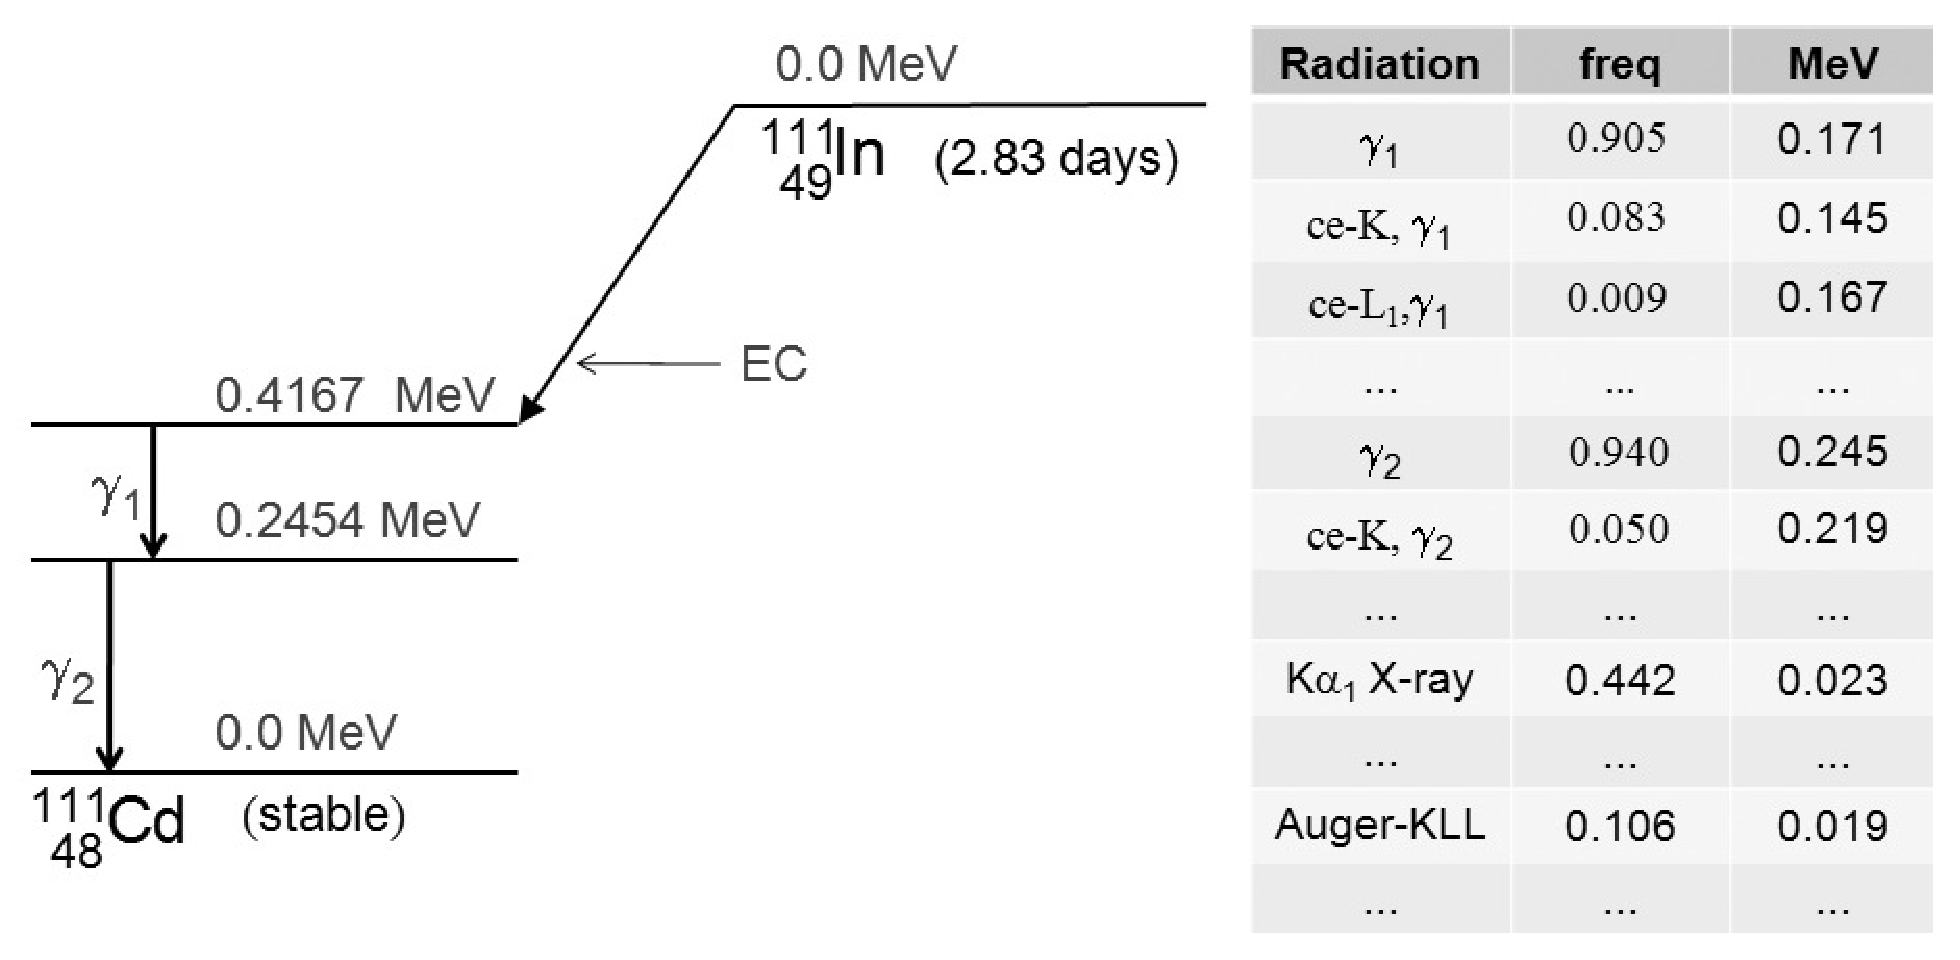
\includegraphics[width = 0.8\textwidth]{figs/fig_In111.pdf}
\caption{\label{fig:In111} \emph{Decay scheme of $^{111}$In, by
    electron capture. The scheme is dominated by the emission of two
    gamma rays (171 and 245 keV). These gamma rays can be involved in
    production of conversion electrons. A more complete table is given
    in \cite{Cherry}.}}
\end{figure}

\item Positron emission ($\beta^+$ decay).\\
\begin{itemize}
\item A proton is transformed into a neutron and a positron (or
anti-electron):
\begin{equation}
  p^+ \rightarrow n + e^+ + \nu_e + \mbox{kinetic energy}.
\end{equation}
After a very short time the positron will hit an electron and annihilate
(fig. \ref{fig:jnpos}).  The mass of the two particles is converted into
energy, which is emitted as two photons. These photons are emitted in opposite
directions. Each photon has an energy of 511 keV (the rest mass of an electron
or positron).


\begin{figure}[tb]
\centering
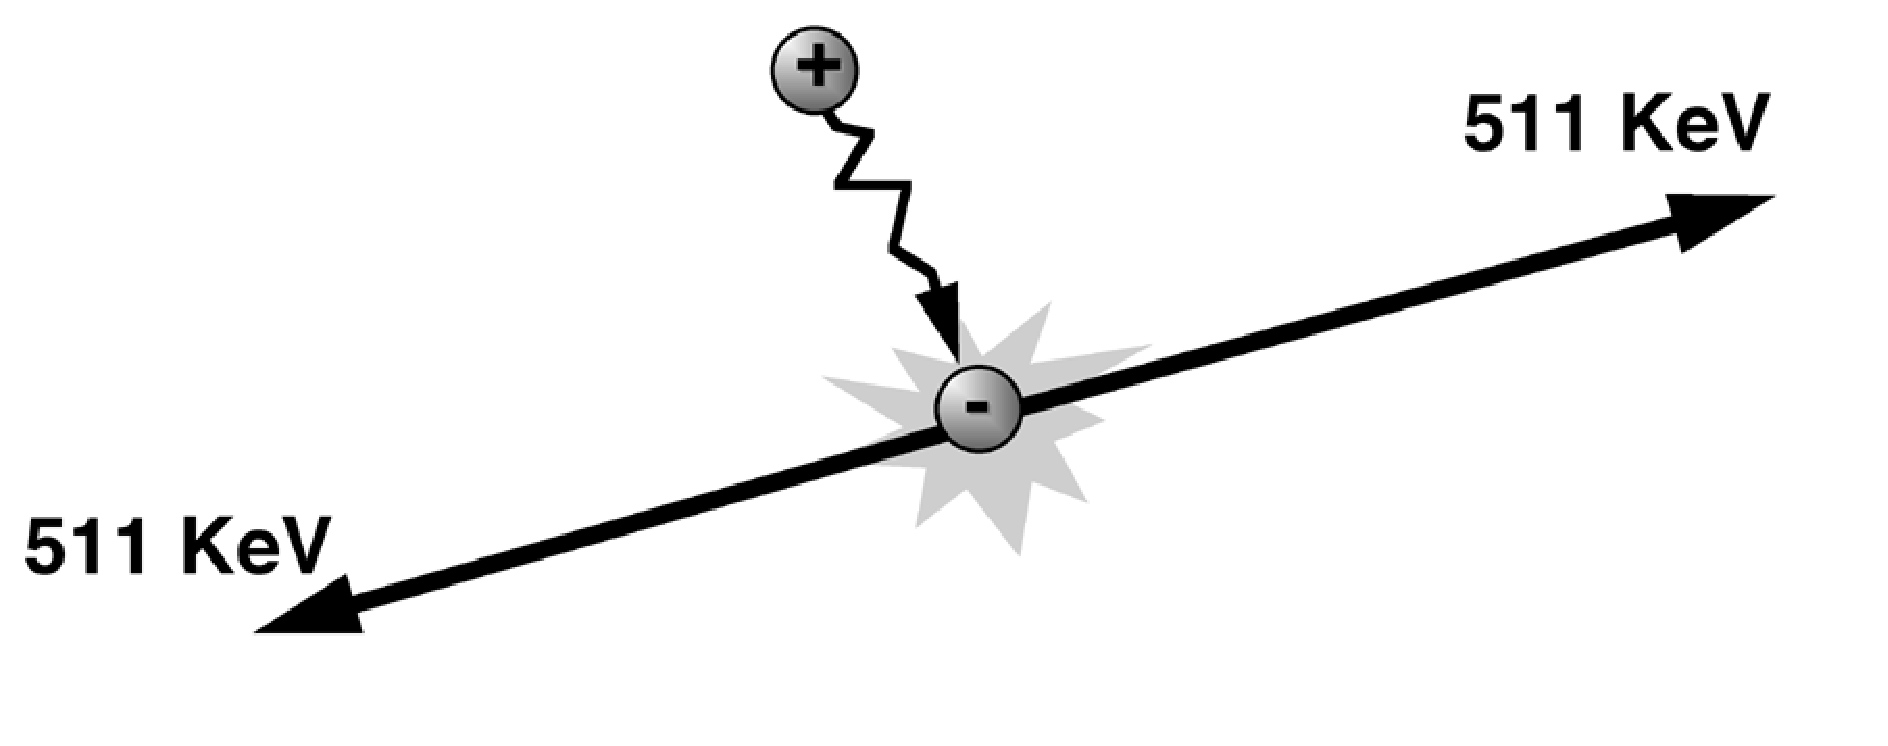
\includegraphics[width = 0.5\textwidth]{figs/fig_jnpos.pdf}
\caption{\label{fig:jnpos} \emph{Positron-electron annihilation.}}
\end{figure}


\item Again, the daughter nucleus may also be in an excited or a metastable
state.

\end{itemize}
\end{enumerate}
As a rule of thumb, light atoms tend to emit positrons, heavy ones
tend to prefer other modes, but there are exceptions. The most
important isotopes used for positron emission imaging are $^{11}$C,
$^{13}$N, $^{15}$O and $^{18}$F. Since these atoms are very frequent
in biological molecules, it is possible to make a radioactive tracer
which is chemically identical to the target molecule, by substitution
of a stable atom by the corresponding radioactive isotope. These
isotopes are relatively short lived: $^{11}$C: 20 min, $^{13}$N: 10
min, $^{15}$O: 2 min and $^{18}$F: 2 hours. As a result, except for
$^{18}$F, they must be produced close to the PET-system immediately
before injection. To produce the isotope, a small cyclotron is
required. The isotope must be rapidly incorporated into the tracer
molecule in a dedicated radiopharmacy laboratory. In contrast,
$^{18}$F can be transported from the production site to the
hospital. That makes it the most popular isotope in PET.

In nuclear medicine, we use radioactive isotopes that emit photons with an
energy between 80 and 300 keV for single photon emission, and 511 keV for
positron emission. The energy of the emitted photons is fixed: each isotope
emits photons with one or a few very sharp energy peaks. If more than one peak
is present, each one has its own probability which is a constant for that
isotope. So if we administer a tracer to a patient, we know exactly what
photons we will have to measure.


\section{Statistics \label{sec:statistics}}
%%%%%%%%%%%%%%%%%%%%%%%%%%%%%%%%%
The exact moment at which an atom will decay cannot be predicted. All that is
known is the probability that it will decay in the next time interval $dt$.
This probability is $\alpha dt$, where $\alpha$ is a constant for each
isotope.  So if we have $N$ radioactive atoms at time $t_0$, we expect to
see a decrease $dN$ in the next interval $dt$ of
\begin{equation}
  dN = - N \alpha dt. \label{eq:dN}
\end{equation}
Integration over time yields
\begin{equation}
  N(t) = N(t_0) e^{- \alpha (t - t_0)}. \label{jn:decay}
\end{equation}
This is what we {\em expect}. If we actually measure it, we may obtain a
different value, since the process is statistical. As shown below, the
estimate will be better for larger $dN/dt$.

The amount of radioactivity is not expressed as the number of
radioactive atoms present, but as the number of radioactive atoms
decaying per unit of time. From (\ref{eq:dN}) we find that
\begin{equation}
  \mbox{radioactivity} = -\frac{dN}{dt} = \alpha N =
  \frac{N}{t_{\frac{1}{2}}} \ln 2.
\end{equation}
Therefore, for the same amount of radioactivity, more radioactive
atoms are needed if the half life is longer.  This quantity used to be
expressed in Curie (Ci), but the preferred unit is now Becquerel (Bq)
\footnote{Marie and Pierre Curie and Antoine Becquerel received the
Nobel prize in 1903, for their discovery of radioactivity in 1896}.
One Bq means 1 event per s. For the coming years, it is useful to know
that
\begin{equation}
 1 \ \mbox{mCi} = 37 \ \mbox{MBq} = 37 \times 10^{6} / \mbox{s}.
\end{equation}
The amounts of radioactivity used in nuclear medicine imaging are
typically in the order of $10^2$ Mbq.

The half life of a tracer is the amount of time after which only half the
amount of radioactivity is left. It is easy to compute it from equation
(\ref{jn:decay}):
\begin{equation}
 t_{\frac{1}{2}}  = \frac{\ln 2}{\alpha} .
\end{equation}

As shown in appendix \ref{app:poisson}, the probability of measuring $n$
photons, when $r$ photons are expected equals
\begin{eqnarray}
  p_r(n) & = & \frac{e^{-r} r^n}{n!}  \label{jn:Poisson} \\
         & = & e^{-r} \frac{r}{1} \frac{r}{2} \frac{r}{3} \ldots \frac{r}{n}
\end{eqnarray}
This is a Poisson distribution with $r$ the average number of expected
photons. The mean of the distribution is $r$, and the standard
deviation equals $\sqrt{r}$. For large $r$, it can be well
approximated by a Gaussian with mean $r$ and standard deviation
$\sqrt{r}$:
\begin{equation}
  p_r(n) \simeq \frac{1}{\sqrt{2 \pi r}} \exp \left( \frac{- (n - r)^2}{2 r} 
  \right)
\end{equation} For smaller ones (less than 10 or so) it becomes markedly
asymmetrical, since the
probability is always $0$ for negative values.

Note that the distribution is only defined for integer values of $n$. This is
obvious, because one cannot detect partial photons ($r$ is a real number,
because the average number of expected photons does not have to be integer).
Summing over all $n$ values yields
\begin{equation}
 \sum_0^\infty p_r(n) = e^{-r} \sum_0^\infty \frac{r^n}{n!}
  = e^{-r} e^{r} = 1.
\end{equation}
As with a Gaussian, $r$ is not only the mean of the distribution, it is also
the value with highest probability.

When one estimates radioactivity by counting emitted photons (or other
particles), the signal-to-noise ratio (SNR) of that measurement equals
\begin{equation}
 SNR = \frac{r}{\sqrt{r}} = \sqrt{r},
\end{equation}
where $r$ is the expection of the number of measured photons.  Hence,
if we measure the amount of radioactivity with particle detectors, the
SNR becomes larger if we measure longer.

The only assumption made in the derivation in appendix
\ref{app:poisson} was that the probability of an event was constant in
time. It follows that ``thinning'' a Poisson process results in a new
Poisson process. With thinning, we mean that we randomly accept or
reject events, using a fixed acceptance probability. If we expect $N$
photons, and we randomly accept with a probability $f$, then the
expected number of accepted photons is $fN$. Since the probability of
surviving the whole procedure (original process followed by selection)
has a fixed probability, the resulting process is still Poisson.

\chapter{Interaction of photons with matter}

\begin{figure}[tb]
\centering
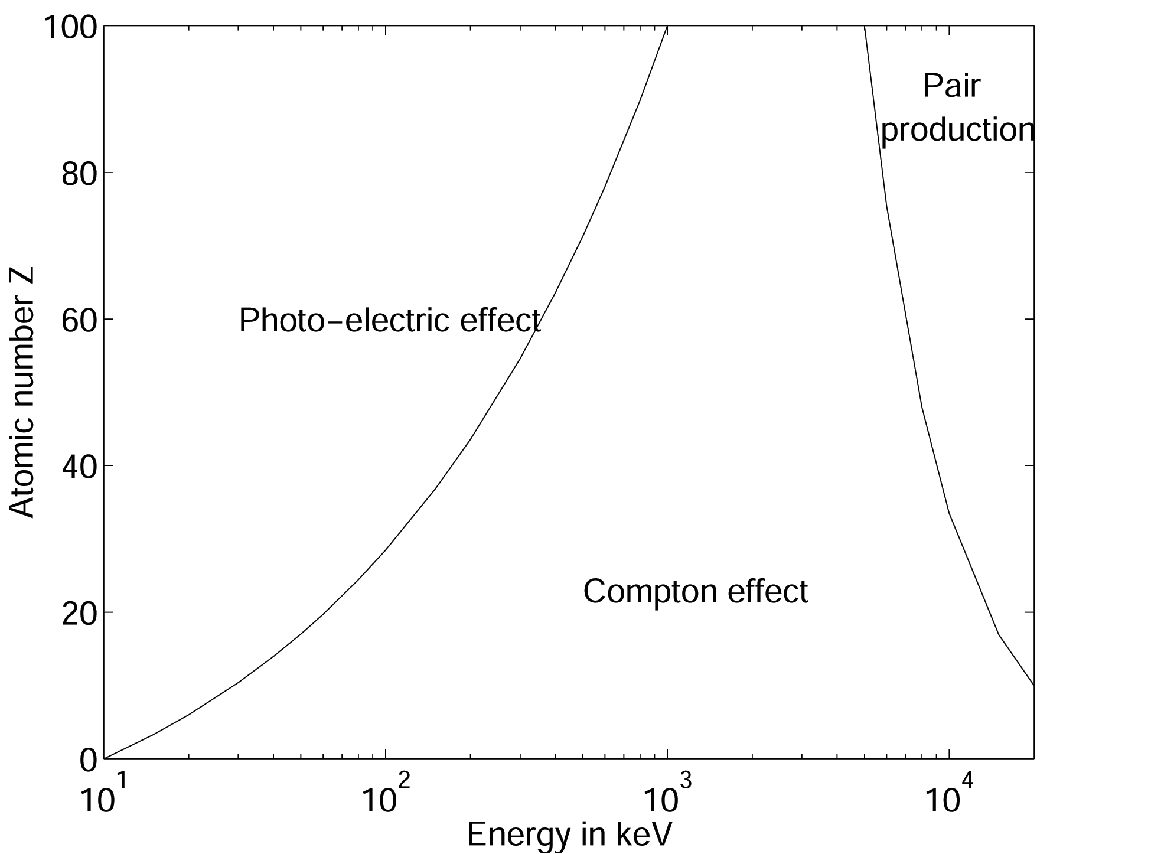
\includegraphics[width = \figone]{figs/fig_foto_compton_pair.pdf}
\caption{\label{fig:foto_compton_pair} \emph{Dominating interaction as a
function of electron number Z and photon energy.}}
\end{figure}

In nuclear medicine, photon energy ranges roughly from 60 to 600 keV. For
example, \Tc\ has an energy of 140 keV. This corresponds to a wave
length of 9~pm and a frequency of 3.4 $\times$ $10^{19}$ Hz. At such energies,
$\gamma$ photons behave like particles rather than like waves.

At these energies, the dominating interactions of photons with matter are
photon-electron interactions: Compton scatter and photo-electric effect. As
shown in figure \ref{fig:foto_compton_pair}, the dominating interaction is a
function of energy and electron number. For typical nuclear medicine
energies, Compton scatter dominates in light materials (such as water and
human tissue), and photo-electric effect dominates in high density materials.
Pair production (conversion of a photon in an electron and a positron) is
excluded for energies below 1022 keV, since each of the particles has a mass
of 511 keV. Rayleigh scatter (absorption and re-emission of (all or a
fraction of) the absorbed energy as a photon in a different direction) has a
low probability.

\section{Photo-electric effect}
%%%%%%%%%%%%%%%%%%%%%%%%%%%%%%%%%
A photon ``hits'' an electron, usually from an inner shell (strong
binding energy). The electron absorbs all the energy of the photon. If
that energy is higher than the binding energy of the electron, the
electron escapes from its atom. Its kinetic energy is the difference
between the absorbed energy and the binding energy. In a dense
material, this photo-electron will collide with electrons from other
atoms, and will lose energy in each collision, until no kinetic energy
is left.

As a result, there is now a electron vacancy in the atom, which may be filled
by an electron from a higher energy state. The difference in binding energy
of the two states must be released. This can be done by emitting a photon.
Alternatively, the energy can be used by another electron with low binding
energy to escape from the atom.

In both cases, the photon is completely eliminated.

The probability of a photo-electric interaction is approximately proportional
to $Z^3 / E^3$, where $Z$ is the atomic number of the material, and $E$ is the
energy of the photon. So the photo-electric effect is particularly important for
low energy radiation and for dense materials.

\section{Compton scatter \label{sec:compton_scatter}}
%%%%%%%%%%%%%%%%%%%%%%%%%%%%%%%%%%%%%%%%%%%%%%%%%%%%%
\begin{figure}[tb]
\centering
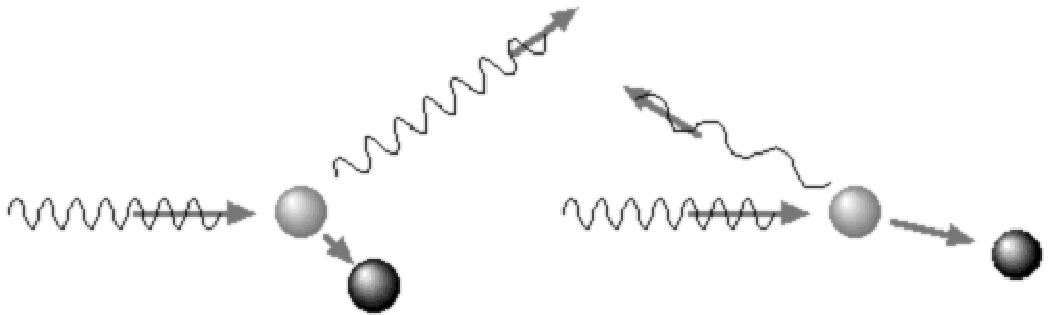
\includegraphics[width=\figone]{figs/fig_compton_scatter.pdf}
\caption{\label{fig:compton_scatter} \emph{Compton scatter can be regarded as
an elastic collision between a photon and an electron.}}
\end{figure}

Compton scatter can be regarded as an elastic collision between a
photon and an electron. This occurs with loosely bound electrons
(outer shell), which have a binding energy that is negligible compared
to the energy of the incident photon. The term ``elastic'' means that
total kinetic energy before and after collision is the same. As in any
collision, the momentum is preserved as well. Applying equations for
the conservation of momentum and energy (with relativistic
corrections) results in the following relation between the photon
energy before and after the collision:
\begin{equation}
  E'_\gamma \;\;=\;\; E_\gamma \frac{1}{1 
     + \Frac{E_\gamma}{m_e c^2} (1 - \cos\theta)} \label{eq:jn_compton_energy}
   \;\; = \;\; E_\gamma \; P(E_\gamma, \theta)
\end{equation}
%
$\begin{array}{llrl}
\mbox{with}
            & E'_\gamma & = & \mbox{energy after collision}\\
            & E_\gamma  & = & \mbox{energy before collision}\\
            & m_e       & = & \mbox{electron rest mass}\\
            & \theta    & = & \mbox{scatter angle}
\end{array}$\\
%
The expression $m_e c^2$ is the energy available in the mass of the
electron, which equals 511 keV. For a scatter angle $\theta$ = 0, the
photon loses no energy and it is not deviated from its original
direction: nothing happened.  The loss of energy increases with
$\theta$ and is maximum for an angle of 180$^{\circ}$. The probability
that a photon will interact at all with an electron depends on the
energy of the photon. If the interaction takes place, each scatter
angle has its own probability, and this probability is proportional to
the differential cross section, given by the Klein-Nishina equation:
\begin{equation}
 \frac{d\sigma}{d\Omega} = \frac{1}{2} r_e^2 \; P(E_\gamma, \theta)^2
    \left( P(E_\gamma, \theta) + \frac{1}{P(E_\gamma, \theta)} - \sin^2\theta \right),
    \label{eq:kleinnishina}
\end{equation}
where $r_e$ is the classical electron radius and $P(E_\gamma, \theta)$
is defined above. The cross section $\sigma$ has the unit of area,
$\Omega$ is the solid angle. Integrating over $\Omega$
would produce the total cross section for Compton scatter. For that
integration, $d\Omega$ can be written as $2 \pi \sin\theta \,d\theta$
\footnote{If you are not sure why, this is explained in the derivation
  of equation (\pref{eq:wellcounter}).}.
The differential cross section (\ref{eq:kleinnishina}) is shown for a
few incoming photon energies in figure \ref{fig:kleinnishina}. For
higher energies, smaller scatter angles become increasingly likely.

\begin{figure}[htb]
\centering
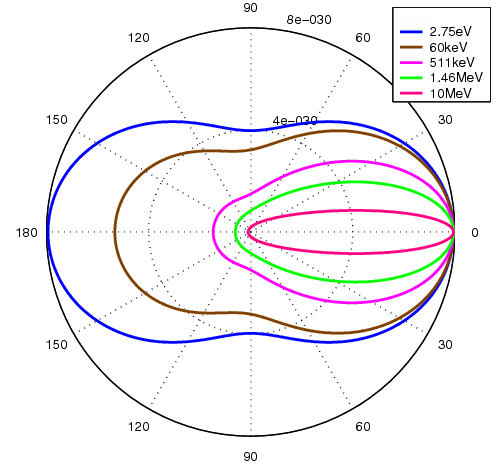
\includegraphics[bb=0 0 500 473,width=\figmedium]{figs/fig_klein_nishina.png}
\caption{\label{fig:kleinnishina} \emph{The scattering-angle
    distribution for a few photon energies. Figure from Wikipedia
    (https://en.wikipedia.org/wiki/Klein-Nishina\_formula).}}
\end{figure}


The probability of a Compton decreases very slowly with increasing $E$
(see fig. \ref{fig:atten_water}) and with increasing $Z$.

Because the energy of the photon after scattering is less than before,
Compton scatter is sometimes also called ``inelastic scattering''.

\section{Rayleigh scatter}
%%%%%%%%%%%%%%%%%%%%%
Rayleigh scattering or coherent scattering can be regarded as the
collision between a photon and an entire atom. Because of the huge
mass of the atom, the photon is deflected from its original trajectory
without any noticeable loss of energy (replace $m_e c^2$ with $\infty$
in (\ref{eq:jn_compton_energy})). Rayleigh scattering contributes only
significantly at low energies, and can be safely ignored in typical nuclear
medicine applications. Because the energy of the photon after
scattering is the same as before, this effect is also called ``elastic
scattering''.

\section{Attenuation}
%%%%%%%%%%%%%%%%%%%%%

\begin{figure}[tb]
\centering
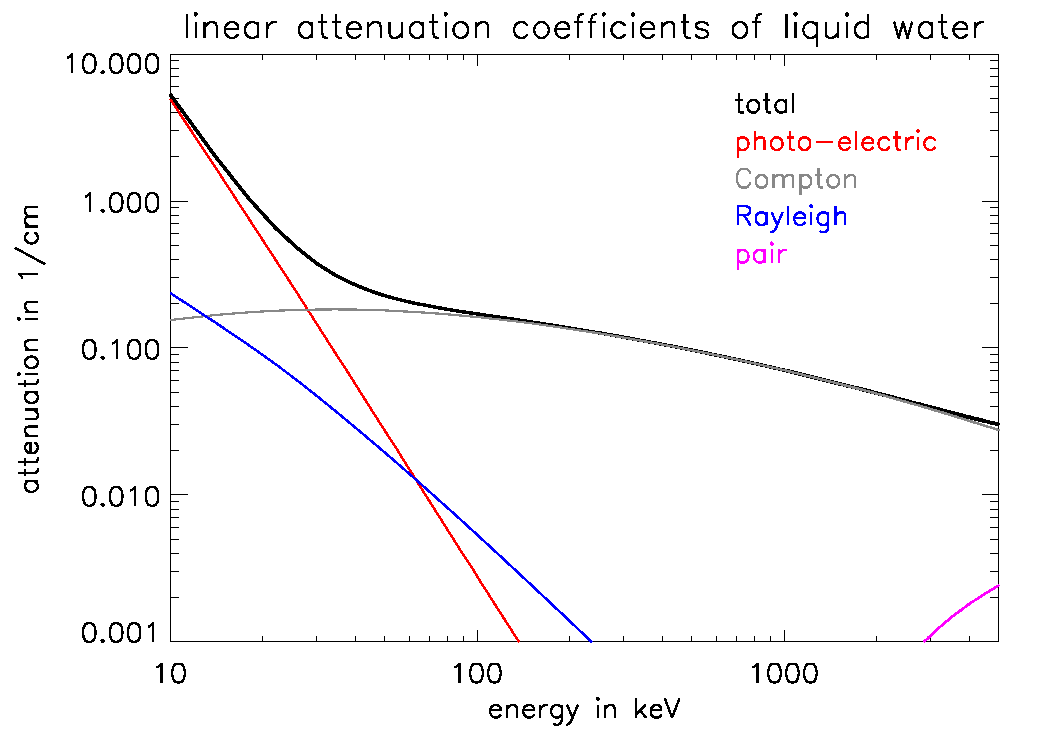
\includegraphics[width=\figmedium]{figs/fig_atten_water.pdf}
\caption{\label{fig:atten_water} \emph{Photon attenuation in water as a
function of photon energy. The photo-electric component decreases
approximately with $(Z/E)^3$ (of course, $Z$ is a constant here). The Compton
components varies slowly.}}
\end{figure}

The {\em linear attenuation coefficient} $\mu$ is defined as the
probability of interaction per unit length (unit: cm$^{-1}$). Figure
\ref{fig:atten_water} shows the mass attenuation coefficients as a
function of energy in water. Multiply the mass attenuation coefficient
with the mass density to obtain the linear attenuation
coefficient. When photons are traveling in a particular direction
through matter, their number will gradually decrease, since some of
them will interact with an electron and get absorbed (photo-electric
effect) or deviated (Compton scatter) into another direction. By
definition, the fraction that is eliminated over distance $ds$ equals
$\mu(s) N(s)$:
\begin{equation}
  dN(s) = - \mu(s) N(s) ds. \label{eq:diff_atten}
\end{equation}

If initially $N(a)$ photons are emitted in point $s = a$ along the $s$-axis,
the number of photons $N(d)$ we expect to arrive in the detector at position
$s = d$ is obtained by integrating (\ref{eq:diff_atten}):
\begin{equation}
  N(d) = N(a) \  e^{- \int_a^d \mu(s) ds}. 
\label{jn:spectatten}
\end{equation}
Obviously, the attenuation of a photon depends on where it has been emitted.

\begin{figure}[tb]
\centering
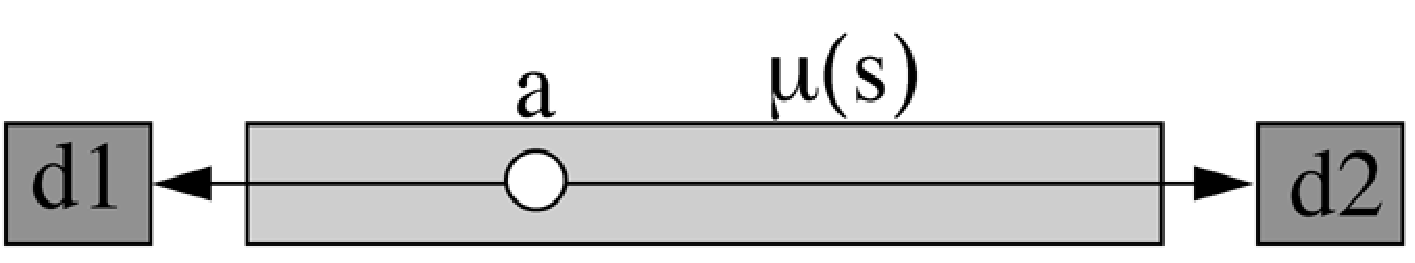
\includegraphics[width=\figone]{figs/fig_jnpetatten.pdf}
\caption{\label{fig:jn_petatten} \emph{Positron emitting point source in a
non-uniform attenuator.}}
\end{figure}
For positron emission, a pair of photons need to be detected. Since the fate
of both photons is independent, the detection probabilities must be
multiplied.  Assume that one detector is positioned in $s = d_1$, the second
one in $s = d_2$, and a point source in $s = a$, somewhere between the two
detectors. Assume further that during a measurement, $N(a)$ photon pairs were
emitted along the $s$-axis (fig.\ref{fig:jn_petatten}). The number of
detected pairs then is:
\begin{equation}
  N(d_1,d_2) = N(a)  e^{- \int_{d_1}^a \mu(s) ds} e^{- \int_a^{d_2} \mu(s)
             ds} \\
             = N(a)  e^{- \int_{d_1}^{d_2} \mu(s) ds}. \\
\label{jn:petatten}
\end{equation}
Equation (\ref{jn:petatten}) shows that for PET, the effect of attenuation is
independent of the position along the line of detection.

Photon-electron interactions will be more likely if there are more electrons
per unit length. So dense materials (with lots of electrons per atom) have a
high linear attenuation coefficient.

\chapter{Data acquisition}

In nuclear medicine, photon detection hardware differs considerably from that
used in CT. In CT, large numbers of photons must be acquired in a very short
measurement. In emission tomography, a very small number of photons is
acquired over a long time period. Consequently, emission tomography systems are
optimized for sensitivity.

Photo-electric absorption is the preferred interaction in the detector, since
it results in absorption of all the energy of the incoming photon. Therefore
the detector material must have a high atomic number (the atomic number Z is
the number of electrons in the atom). Since interaction probability decreases
with increasing energy, a higher Z is needed for higher energies.

In single photon imaging, \textsuperscript{99m}Tc\ is the tracer that is mostly used. It has
an energy of 140 keV and the gamma camera performance is often optimized for
this energy.  Obviously, PET-cameras have to be optimized for 511~keV.

\section{Detecting the photon}
%%%%%%%%%%%%%%%%%%%%%%%%%%%%%%
Different detector types exist, but the current standard, both in SPECT and
PET, is the scintillation detector. The following sections describe the
scintillation crystal, the photomultiplier tube and how crystal and tubes
can be combined to make a two-dimensional gamma detector. After that, some
alternative designs and new developments will be mentioned.

\subsection{Scintillation crystal}
%=================================
A scintillation crystal is a remarkable material that stops the incoming
photon and in doing so produces a flash of visible light, a scintillation.
So the problem of detecting the incoming photon is now transformed in the
easier problem of detecting the light flash.

The scintillation stops the photon via photo-electric absorption or via
multiple scattering events. The resulting photo-electron travels through the
crystal, distributing its kinetic energy over a few thousands other electrons
in multiple collisions. As a result, there will be a few thousands of a
electrons in an excited state. After a short time, these electrons will
release their energy in the form of a photon of a few eV. These secondary
photons are visible to the human eye (they are usually blue): this is the
scintillation.

The exact wavelength (or color) of the light flash depends on the crystal,
but {\em not} on the energy of the incoming high-energy photon. If a photon
with a higher energy enters the crystal, it will send more electrons to an
higher energy level. Each of these electrons will then produce a single
scintillation-photon, always with the same color. So if we want to have an
idea about the energy of the incoming photon, we need to look at the number
of scintillation photons (the intensity of the flash), and not at their
energy (the color of the flash).

Many scintillators exist, and quite some research on new scintillators
is still going on. The crystals that are mostly used today are NaI(Tl)
for single photons (140 keV) in gamma camera and SPECT, and LSO
(lutetium oxyorthosilicate) for annihilation photon (511 keV) in
PET. Before LSO was found, BGO (bismuth germanate) was used for PET,
and there are still some old BGO-based PET systems around. Some other
crystals, such as GSO (gadolinium oxyorthosilicate) and LYSO (LSO with
a bit of Yttrium, very similar to LSO) are used for PET as well. The
important characteristics of the crystals are:
\begin{itemize}
  \item Transparency. If it is not transparent, we cannot see or detect the
        light flash.
  \item Photon yield per incoming keV. More photons per keV is better, since
        the light flash will be easier to see. The scintillation and
        its detection are statistical processes, and the uncertainty
        associated with it will go down if the number of scintillation
        photons increases.
  \item Scintillation time. This is the average time that the electrons
        remain in the excited state before releasing the scintillation
        photon. Shorter is better, since we want to be ready for the next
        photon.
  \item Attenuation coefficient for the high energy photon. We want to stop
        the photon, so a higher attenuation coefficient is better. Denser
        materials tend to stop better.
  \item Wave length of the scintillation light. Some wave lengths are easier
        to detect than others.
  \item Ease of use: some crystals are very hygroscopic: a bit of water
        destroys them. Others can only be produced at extremely high
        temperatures. And so on.
\end{itemize}

\begin{table}
\centering
\caption{Characteristics of a few scintillation crystals.}
\label{tab:crystals}
\begin{tabular}{|c|c|c|c|c|}
\hline
       & NaI(Tl) &    BGO      & LSO      & GSO \\
\hline
Photons per keV                    
        &  40     & 5 \ldots 8  & 20 \ldots 30 &  12\\
Scintillation decay time [ns]
        & 230     &  300  & 40  & 65 \\
Linear atten. coeff. [/cm] (at 511 keV)
        & 0.34    & 0.95  & 0.87  & 0.67\\
 Wave length [nm]
        & 410     & 480   & 420 & 440 \\
Melting temperature ($^o$C)
        & 651 & 1050 & 2050 & 1950 \\
\hline
\end{tabular}
\begin{itemize}
\item NaI(Tl): NaI crystal doped with Tl
\item BGO: Bi$_4$Ge$_{3}$O$_{12}$
\item LSO: Lu$_2$SiO$_5$
\item GSO: Gd$_2$SiO$_5$ doped with Ce
\end{itemize}
\end{table}

The scintillation photons are emitted to carry away the energy set
free when an electron returns to a lower energy level. Consequently,
these photons contain just the right amount of energy to drive an
electron from a lower level to the higher one. In pure NaI this
happens all the time, so the photons are reabsorbed and the
scintillation light never leaves the crystal. To avoid this, the NaI
crystal is doped with a bit of Tl (Thallium). This disturbs the
lattice and creates additional energy levels. Electrons returning to
the ground state via these levels emit photons that are not
reabsorbed.  NaI is hygroscopic (similar as NaCl (salt)), so it must
be protected against water. LSO has excellent characteristic, but is
difficult to process (formed at very high temperature), and it is
slightly radioactive. Table \ref{tab:crystals} lists some
characteristics of three scintillation crystals.

\subsection{Photo Multiplier Tube}
%=================================
The scintillation crystal transforms the incoming photon into a light flash.
That flash must be detected. In particular, we want to know {\em where} it
occurred, {\em when} it occurred and {\em how intense} it was (to compute the
energy of the incoming photon). All this is usually obtained with
photomultiplier tubes (PMT).

\begin{figure}[tb]
\centering
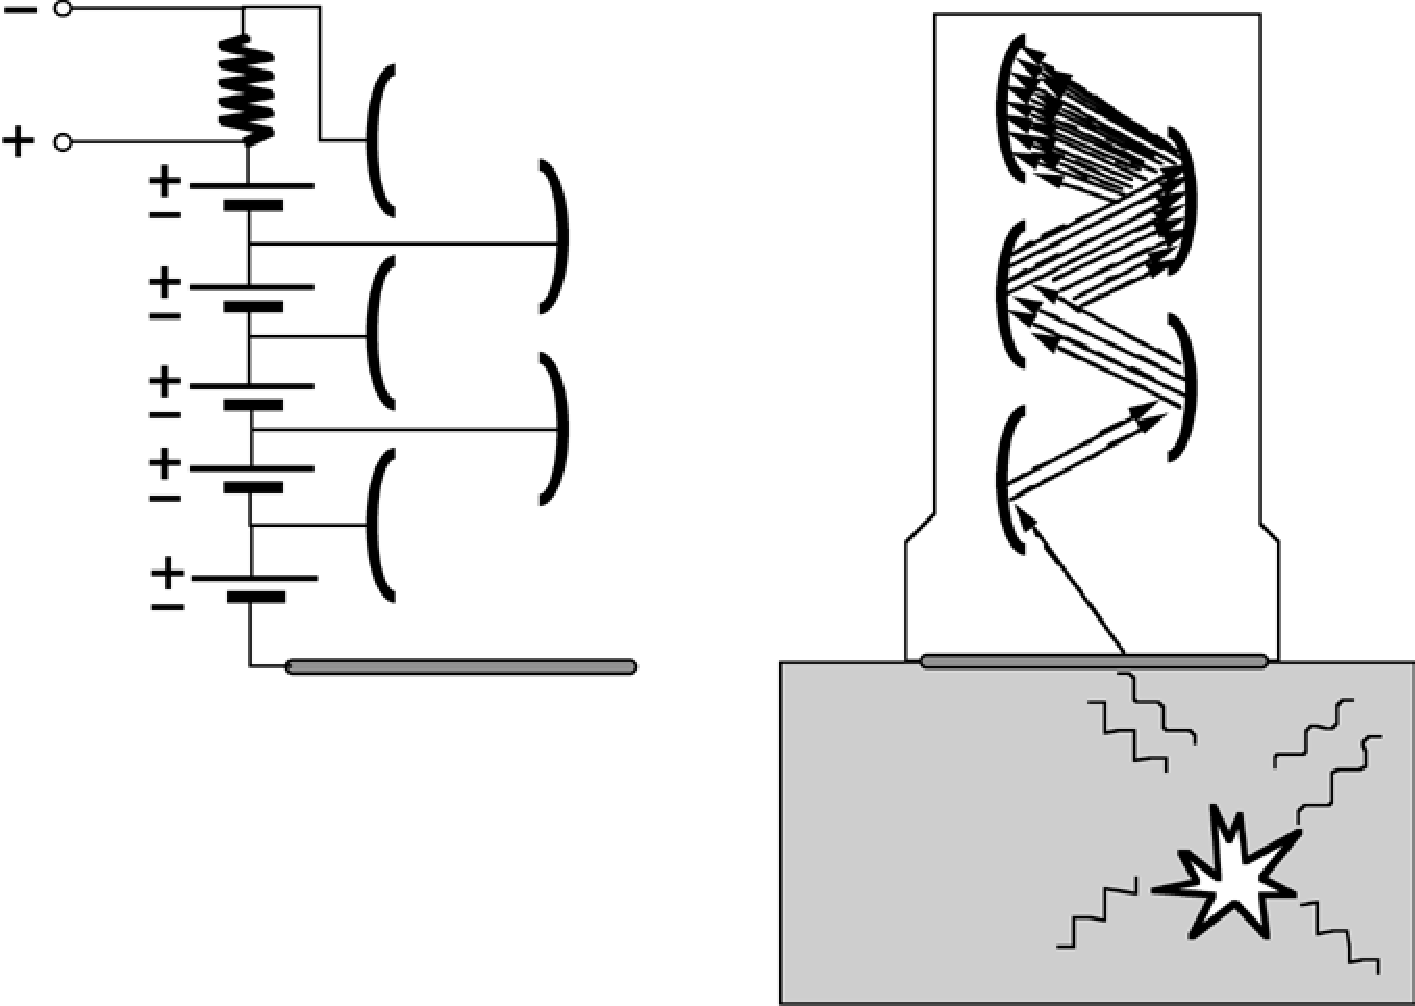
\includegraphics[width=0.5\textwidth]{figs/fig_jnpmt.pdf}
\caption{\label{fig:jnpmt} \emph{Photomultiplier. Left: the electrical scheme.
Right: scintillation photons from the crystal initiate an electric current to
the dynode, which is amplified in subsequent stages.}}
\end{figure}

The PMT's are glued onto the crystal, in order to detect the incoming
scintillation photons. The PMT consists of multiple dynodes, the first of
which (the photocathode) is in optical contact with the crystal. High negative
voltage (in the order of 100 V) between the dynodes makes the electrons want
to jump from one to the other, but they do not have enough energy to cross the
gap in between (fig \ref{fig:jnpmt}).  This energy is provided by the
scintillation photon. The electron acquiring the threshold energy will be
accelerated by the electrical field, and activate multiple electrons in the
next dynode. After a few steps, a measurable voltage is created which is
digitized with an analog-to-digital converter. There are usually about 10 to
12 dynodes, and each step amplifies the signal with a factor 3 \ldots 6, so
amplification can be in the order of one million.

The response time of a PMT is very short (a few ns) compared to the
scintillation decay time.


\subsection{Two-dimensional gamma detector}
%==========================================
% Single crystal vs multicrystal
% position (intrinsic resolution), energy (-resolution)
% constant fraction discriminator.
%
There are two ways to build a two-dimensional gamma detector based on
scintillation. One way is to use a single very large crystal and connect
multiple PMT's to it. The other way is to combine small crystals in a
large matrix.

\subsubsection{Single crystal detector} \label{sec:single_crystal}
%------------------------------------
This is the standard design for single photon detectors with NaI(Tl). One
side of a single large crystal (e.g. 50 cm x 40 cm, 1 cm thick) is covered
completely with PMT's (\ldots 50 \ldots PMTs). The other side is covered with
a layer acting as a mirror for the scintillation photons, so that as many as
possible are collected in the PMT's.

In principle, all PMT's contribute to the detection of a single
scintillation event. As mentioned before, the position, the time and the
energy ( $\sim$ amount of scintillation photons) must be computed from the
PMT-outputs.
%
\begin{itemize}

\item {\bf Position:} $(x,y)$\\
The x-position is computed as
\begin{equation}
x = \frac{\sum_i x_i S_i}{\sum_i S_i}, \label{eq:gammaposition}
\end{equation}
where $i$ is the PMT-index, $x_i$ the $x$-position of the PMT and $S_i$ the
integral of the PMT output over the scintillation duration.  The $y$-position
is computed similarly. Expression (\ref{eq:gammaposition}) is not very
accurate and needs correction for systematic errors (linearity correction).
The reason is that the response of the PMT's does not vary nicely with the
distance to the pulse. In addition, each PMT behaves a bit differently. This
will be discussed later in this chapter.

\item {\bf Energy:} $E$\\
The energy is computed as
\begin{equation}
 E = c_E {\sum_i S_i}
\end{equation}
where $c_E$ is a coefficient converting voltage (integrated PMT output) to
energy. The ``constant'' $c_E$ is not really a constant: it varies slightly
with the energy of the high energy photon. Moreover, it depends also on
the position of the scintillation, because of the complex and individual
behavior of the PMT's. Compensation of all these effects is called ``energy
correction'', and will be discussed below.

\item {\bf Time: } $t$\\
In positron emission tomography, we must detect pairs of photons which have
been produced simultaneously during positron-electron annihilation.
Consequently, the time of the scintillation must be computed as accurately as
possible, so that we can separate truly simultaneous events from events that
happen to occur almost simultaneously.

The scintillation has a finite duration, depending on the scintillator
(see table \ref{tab:crystals}).  The scintillation duration is
characterized by the the decay time $\tau$, assuming that the number
of scintillation photons decreases as $\exp(- t/\tau)$. The decay
times of the different scintillation crystals are in the range of 40
to several 100 ns. This seems short, but since a photon travels about
1 meter in only 3.3 ns, we want the time resolution to be in the order
of a few ns (e.g. to suppress the random coincidence rate in PET, as
will be explained in section \ref{sec:septa}). To assign such a
precise time to a relatively slow event, the electronics typically
computes the time at which a predefined fraction of the scintillation
light has been collected (constant fraction discriminator). In current
time-of-flight PET systems based on LSO, one obtains a timing
resolution of about 400 ps.

\end{itemize}

\subsubsection{Multi-crystal detector matrix}
%------------------------------------
Instead of using a single large crystal, a large detector area can be
obtained by combining many small crystals in a two-dimensional
matrix. The crystals should be optically separated (such that
scintillation photons are mirrored at the edges), to make sure that
the scintillation light produced in one crystal stays in that
crystal. In the extreme case, each crystal has its own
photomultiplier. Computation of position is ``trivial'' (although
complicated in practice): it is the coordinate of the crystal in the
matrix (no attempt is made to obtain sub-crystal accuracy). Energy is
proportional to the total output of the PMT coupled to the crystal. In
such a design, the top of the crystal is usually a square of 3 to 5
mm, and the crystal is a cm (140 keV) or a few cm (511 keV) thick.
Consequently, the spatial resolution is about 4 mm, as in the single
crystal case (see section \ref{sec:resolution}).

\begin{figure}[tb]
\centering
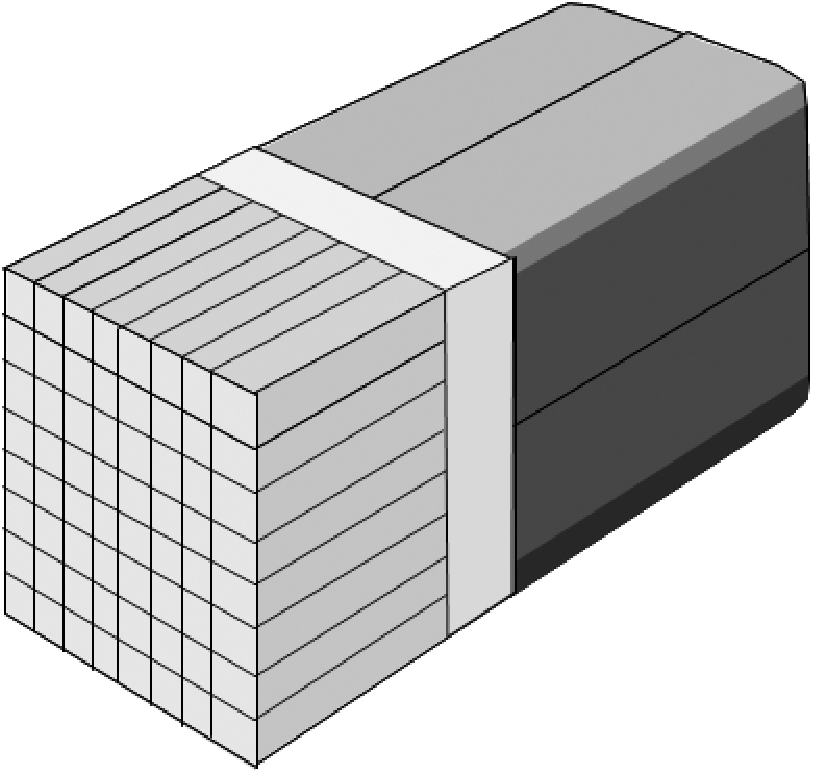
\includegraphics[width=0.3\textwidth]{figs/fig_multicrystal.pdf}
\caption{\label{fig:multicrystal} \emph{Multi-crystal module. The outputs
of four photomultipliers are used to compute in which of the 64 crystals
the scintillation occurred.}}
\end{figure}

Photomultipliers are expensive, so the manufacturing cost can be
reduced by a more efficient use of the PMT's. Figure
\ref{fig:multicrystal} shows a typical design, where a matrix of 64
(or more) crystals is connected to only four multipliers. The
transparent block between the crystals and the PMT is called the {\em
light guide}.  It guides the light towards the PMT's in such a way
that the PMT amplitude changes monotonically with distance to the
scintillating crystal. Thus, the relative amplitudes of the four
PMT-outputs allow to compute in which crystal the scintillation
occurred. For PET, the crystals have typically a cross section of
about 4mm $\times$ 4 mm, and they are about 2 cm long.

In a single crystal design, all PMT's contribute to the detection of a single
scintillation. If two photons happen to hit the crystal simultaneously, both
2scintillations will be combined in the calculations and the resulting energy
and position will be wrong! Thus, the maximum count rate is limited by the
decay time of the scintillation event. In a multi-crystal design, many modules
can work in parallel, so count rates can be much higher than in the single
crystal design. Count rates tend to be much higher in PET than in SPECT or
planar single photon imaging (see below). That is why most PET-cameras are
using the multicrystal design, and gamma cameras are mostly single crystal
detectors. However, single crystal PET systems and multi-crystal gamma cameras
exist as well.


\subsection{Resolution} \label{sec:resolution}
%=================================
The coordinates $(x, y, E, t)$ can only be measured with limited precision.
They depend on the actual depth where the incoming photon was stopped, on
the number of electrons that was excited, on the time the electrons remain
in the excited state, on the direction in which each scintillation photon is
emitted when the electron returns to a lower energy state and on the amount of
electrons that is activated in the PMT's in each dynode. These are all
random processes: if two identical high energy photons enter the crystal at
exactly the same position, all the forthcoming events will be different. We
can only describe them with probabilities.

So if the photon really enters the crystal at $(\bar{x}, \bar{y}, \bar{E},
\bar{t})$, the actual measurement will produce a random realization $(x_i,
y_i, E_i, t_i)$ drawn from a four-dimensional probability distribution
$(x, y, E, t)$. We can measure that probability distribution by doing
repeated measurements in a well-controlled experimental situation. E.g., we
can put a strongly collimated radioactive source in front of the crystal,
which sends photons with the same known energy into the crystal at the same
known position. This experiment would provide us the distribution for $x$,
$y$ and $E$. The time resolution can be determined in several ways, e.g. by
activating the PMT's with light emitting diodes. The resolution on $x$ and $y$
is often called the {\em intrinsic resolution}.

If we plot all the measurements in a histogram, we will see the
distribution. Usually the distribution is approximately Gaussian, and can be
characterized by its standard deviation $\sigma$. Often one specifies the
full width at half maximum (FWHM) instead (figure \ref{fig:fwhm}). It is easy
to show that for a Gaussian, the FWHM $ = 2 \sqrt{2 \ln 2} \sigma$. This
leads to a useful rule of thumb: {\em any detail smaller than the FWHM is lost
during the measurement}.
 
\begin{figure}[tb]
\centering
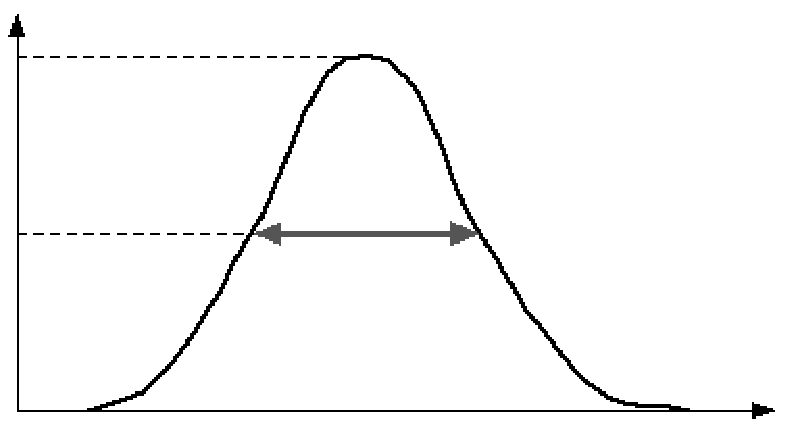
\includegraphics[width=0.35\textwidth]{figs/fig_fwhm.pdf}
\caption{\label{fig:fwhm} \emph{The full width at half max of a probability
distribution}}
\end{figure}

Position resolution of a scintillation detector has a FWHM of 3 to 4 mm.
Energy resolution is about 10\% FWHM (so 14 keV for a 140 keV tracer) in
NaI(Tl) cameras, about 20\% FWHM (about 130 keV at 511 keV) or worse in
BGO PET-systems, and about 15\% FWHM in LSO and GSO PET-systems.

\subsection{Storing the data} \label{sec:storing_data}
%=================================
To store the data, the information must be digitized. We do not want to lose
information, so the round-off errors made during digitization should be small
compared to the resolution. Thus, we obtain four digital numbers $(x, y, E,
t)$, which are the coordinates of a single detected photon. If all information
must be preserved, we can directly store the four numbers in a list (list-mode
acquisition). Obviously, this list may become very long. Often, we do not need
all this information. The energy is usually simply used to decide whether we
will accept or discard the photon, it does not need to be stored (this will be
explained in section \ref{sec:scatter}). Similarly, we often want to
make a single image representing the situation in a certain time interval, so
we only need a single two-dimensional image. To store this information
efficiently, we prepare a zero two-dimensional matrix, an ``empty'' image, and
increment the value at coordinates $x_i, y_i$ for the $i$-th accepted
photon. The number can be interpreted as a brightness, so we can display the
result as an image on the screen. Brightness (or some pseudo-color)
corresponds to tracer concentration.


\subsection{Alternative designs}
%=================================
Although most current gamma cameras and PET systems are based on
scintillation crystals combined with photomultipliers, there are many
other detection systems. Some of these have very good characteristics, but
their acceptance is hampered by the high cost price and, in some cases, by
the fact that new algorithms must be developed before their full potential
can be exploited. In the following, we only mention two promising
technologies. Avalanche photodiodes can replace the PMT, CdZnTe detectors
can replace the entire standard detection system.

\subsubsection{Avalanche photodiodes}
%------------------------------------
A semiconductor is a material in which the large majority of electrons are
strongly bound to the atoms, but not all of them. Some electrons have enough
energy to move freely about as in a metal. As a result, some of the atoms
have lost an electron and have a net positive charge. This phenomenon gives
rise to two types of charge carriers that can support electric current:
electrons and holes. The former are the freely moving electrons. The latter
are the positive vacancies left behind by the electrons. The holes can move,
because an electron from a neighboring atom can jump over to fill in the
vacancy, creating a similar vacancy in the neighboring atom.

Electric current is possible if freely moving electrons or holes are
available. However, if for some reason none of them are available, the
material acts as an insulator.

A diode is a simple electronic device with wonderful behavior. It has
excellent conductivity in one direction, and extremely poor conductivity in
the other.  This remarkable feature is obtained by connecting two very
different types of semiconductor materials, resulting in a very asymmetrical
distribution of charge carriers. When forward voltage is applied, charge
carriers are injected in great numbers, leading to very low resistance. When
reverse voltage is applied, the electrons and holes are pulled away from the
junction, so there is nothing left to support an electric
current. Consequently, it behaves as an insulator in this mode.

In an avalanche photodiode (APD), a very high reverse voltage is applied,
pulling away all charge carriers. However, a photon hitting the diode may
supply enough energy to break the covalent bond of an electron, thus
creating an electron-hole pair. This free electron will move rapidly in the
electric field, releasing other electrons from their bond. Consequently, the
photon creates an avalanche of free electrons, resulting in a measurable
current. The current is proportional to the number of electrons in the
avalanche, which in turn is proportional to the number of
scintillation photons.

APD's can be used to replace the photomultiplier. The advantage is
that they are much smaller, but currently they are still more
expensive than the PMTs. Another advantage is that they can be used in
a strong magnetic field, while PMTs cannot. In hybrid PET/MRI systems,
where the PET is operated inside the MRI-system, APDs or other similar
devices must be used instead of PMTs.

A limitation of the APD is the long response time. Their timing
resolution is not good enough for time-of-flight PET.

\subsubsection{Multi-pixel photon counters (MPPC or SiPM)}
%-------------------------------------------------
A MPPC or Silicon Photomultiplier (SiPM) consists of an array of APDs
which are operated in Geiger mode. This Geiger mode is obtained by
using a relatively high voltage, such that an incoming photon will
always create a maximum avalanche of electrons, independent of its
energy. Thus, each Geiger mode APD can count the number of
scintillation photons it is hit by. Because a single SiPM consists of
many small APDs, the likelihood of multiple photons hitting the same
APD simultaneously is small. Consequently, the SiPM reliably counts
the number of scintillation photons hitting it.

Compared to the regular APD, the SiPM has the advantage of being much
faster, achieving a response time similar to that of analogue
photomultiplier tubes. That makes them fast enough for time-of-flight
PET. Current timing resolution is around 400 ps, and prototypes with
still better timing are currently being developed.

\subsubsection{Solid state detectors}
%------------------------------------
An effect similar to the one described above can be used to directly
detect the high energy photon instead of the scintillation
photons. For this purpose, a material with high stopping power is
required. This is the operating principle of the CdZnTe detector: a
strong electric field drives charge carriers created by the high
energy photon towards a grid of collectors.  Position resolution is
now determined by the size of the collectors. Designs with
sub-millimeter resolution exist. Energy resolution is excellent (3 \%,
as opposed to the 10 \% in NaI(Tl)). The stopping power is similar to
that of NaI(Tl). Currently, the main disadvantage of CdZnTe detectors
is their very high cost.

As will be discussed in the next section, the resolution of a camera is
dominated by the collimator acceptance angle. Consequently, the excellent
spatial resolution of the CdZnTe detector is completely wasted in the
traditional design. Some researchers are studying alternative camera
designs and accompanying algorithms to fully exploit the excellent
performance of this type of detectors.


\section{Collimation}
%%%%%%%%%%%%%%%%%%%%%
% PSF. Combinatie van resoluties.
% PET sensitiever dan spect. Dus hogere count rates bij zelfde activiteit.

At this point, we know how the position and the energy of a photon
impinging on the detector can be determined. Now we need a way to
ensure that the impinging photons will produce an image. In
photography, a lens is used for that purpose. But there are no
easy-to-use lenses to focus the high energy photons used in nuclear
medicine. So we must fall back on a more primitive approach:
collimation. Collimation is the method used to make the detector
``see'' along straight lines. Different tomographic systems use
different collimation strategies, as shown in figure
\ref{fig:spect_pet_ct}.

\begin{figure}[tb]
\centering
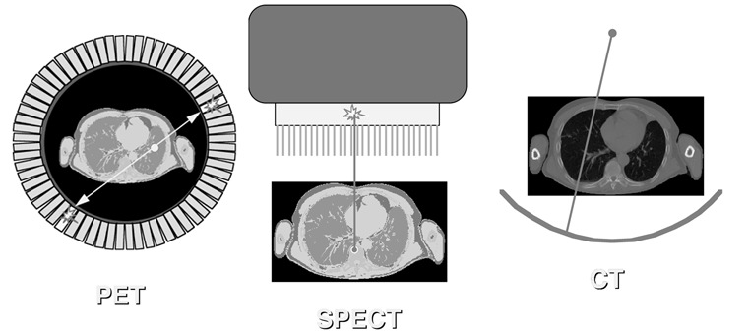
\includegraphics[width=0.75\textwidth]{figs/fig_spect_pet_ct.pdf}
\caption{\label{fig:spect_pet_ct} \emph{Collimation in the PET camera, the
gamma camera (SPECT) and the CT camera.}}
\end{figure}

In the CT-camera, collimation is straightforward: there is only one
transmission source, so any photon arriving in the detector has traveled along
the straight line connecting source and detector. In the PET-camera, a similar
collimation is obtained: if two photons are detected simultaneously, we can
assume they have originated from the same annihilation, which must have
occurred somewhere on the line connecting the two detectors. But for the gamma
camera there is a problem: only one photon is detected, and there is no simple
way to find out where it came from. To solve that problem, mechanical
collimation is used. A mechanical collimator is essentially a thick sieve with
long narrow holes separated by thin septa. The septa are made from a material
with strong attenuation (usually lead), so photons hitting a septum will be
eliminated, mostly by photo-electric interaction. Only photons traveling along
lines parallel to the collimator holes will reach the detector. So instead of
computing the trajectory of a detected photon, we eliminate all trajectories
but one, so that we know the trajectory even before the photon was detected.
Obviously, this approach reduces the sensitivity of the detector, since many
photons will end up in the septa. This is why a PET-system acquires more
photons per second than a gamma camera, for the same activity in the field of
view.

Most often, the parallel hole collimator is used, but for particular
applications other collimators are used as well. Figure \ref{fig:collimators}
shows the parallel hole collimator (all lines parallel), the fan beam
collimator (lines parallel in one plane, focused in the other), the cone beam
collimator (all lines focused in a single point) and the pin hole collimator
(single focus point, but in contrast with other collimators, the focus is
placed {\em before} the object).

\begin{figure}[tb]
\centering
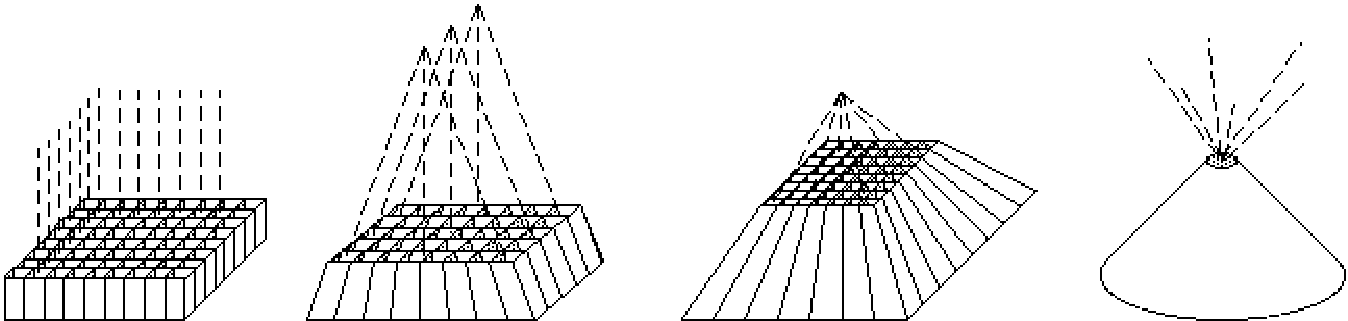
\includegraphics[width=0.6\textwidth]{figs/fig_collimators.pdf}
\caption{\label{fig:collimators} \emph{Parallel hole, fan beam, cone beam and
pin hole collimators.}}
\end{figure}

Collimation ensures that tomographic systems collect information about
lines.  In CT, detected photons provide information about the total
attenuation along the line. In gamma cameras and PET cameras, the
number of detected photons provides information about the total
radioactivity along the line (but of course, this information is
affected by the attenuation as well). Consequently, the acquired
two-dimensional image can be regarded as a set of line integrals of a
three dimensional distribution. Such images are usually called {\em
projections}.

\subsection{Mechanical collimation in the gamma camera} \label{sec:collimation}
%====================================================
Figure \ref{fig:lenscollimator} shows that the sensitivity obtained
with a mechanical collimation is very poor compared to that obtained with a
lens. The mechanical collimator has a dominating effect on the resolution and
sensitivity of the gamma camera. That is why a more detailed analysis of the
collimator point spread function is in order.

\begin{figure}[tb]
\centering
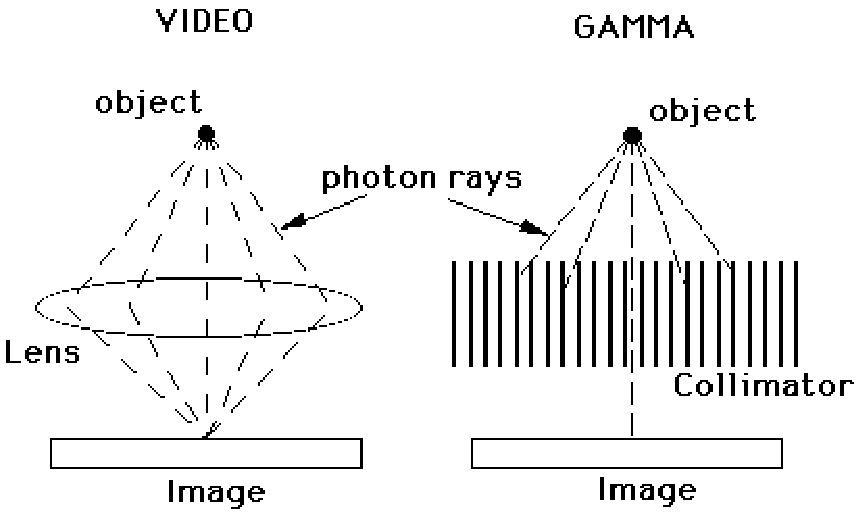
\includegraphics[width=0.5\textwidth]{figs/fig_lenscollimator.pdf}
\caption{\label{fig:lenscollimator} \emph{Focusing by a lens compared to ray
selection by a parallel hole collimator}}
\end{figure}

\begin{figure}[tb]
\centering
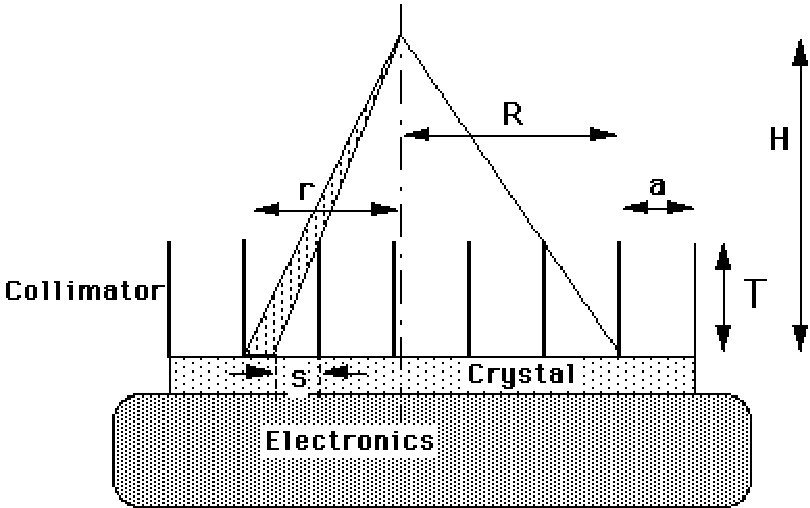
\includegraphics[width=0.5\textwidth]{figs/fig_collimator_calc.pdf}
\caption{\emph{Parallel hole collimator.}}
\label{fig:collimator_calc}
\end{figure}

Fig. \ref{fig:collimator_calc} shows the cross section of a parallel
hole collimator with septa length $T$ and septa spacing $a$. At a
distance of $H$, a radioactive point source is located.  If the
collimator would really absorb all photons except those propagating
exactly perpendicular to the detector, then the image would be a
point.  However, fig. \ref{fig:collimator_calc} shows that photons
propagating along slightly inclined lines may also reach the detector.
Therefore the image will not be a point. Because the image of a point
is characteristic for the system, such images are often studied. By
definition, the image of a point is the {\em point spread function}
(PSF) of the imaging system. 

Assume that the thickness of the septa can be ignored, that $H$ is large
compared to the length of the septa $T$, and that $T$ is large compared to
$a$.  We will also ignore septal penetration (i.e. gamma-photons traveling
through the septa instead of getting absorbed). The light (e.g. 140 keV
photons) emitted by the source makes the septa cast a shadow on the detector
surface. In fact, most of the detector is in that shadow, except for a small
region facing the source. We will regard the center of that region,
immediately under the source, as the origin of the detector plane. The length
of the shadow $s$ cast by a septum on the detector is then
\begin{equation}
s = r \frac{T}{H}
\end{equation}
where $r$ is the distance to the origin. The fraction of the detector element
that is actually detecting photons is
\begin{equation}
f = \frac{a - s}{a} = 1 -  \frac{r T}{a H} = 1 - \frac{r}{R} \label{eq:collim:fraction}
\end{equation}
This expression holds for $r$ between 0 and $R$, where $R$ is the
position at which the shadow completely covers the detector so that $f
= 0$. The expression gives the fraction of the photons detected at
$r$, relative to the number that would be detected at the same
position if there was no collimator. This latter number is easy to
compute. The source is emitting photons uniformly, so the number of
photons per solid angle is constant. Stated otherwise, if we would put
a point source in the center of a spherical uncollimated detector with
radius $H$, the detector surface would be uniformly irradiated. The
total area of the sphere is $4 \pi H^2$, so the sensitivity per unit
area is $1 / (4 \pi H^2)$. Multiplying with the collimator sensitivity
produces the point spread function of the collimated detector at
distance $H$:
\begin{equation}
\mbox{PSF}(r) = (1 -  \frac{r T}{a H}) \frac{1}{4 \pi H^2}
  \label{eq:collim:psf}
\end{equation}
In this expression, we have ignored the fact that for a flat detector, the
distance to the point increases with $r$. The approximation is fair if $r$ is
much smaller than $H$. Consequently, the PSF has a triangular profile, as
illustrated in figure \ref{fig:collimatorpsf}.

To calculate (approximately) the total collimator sensitivity, expression
(\ref{eq:collim:psf}) must be integrated over the region where PSF$(r)$ is
non-zero. We assume circular symmetry and use integration instead of the
summation (actually required by the discrete nature of the problem).
Integration assumes that $a$ and $T$ are infinitely small. Since we use only
the ratio, this poses no problems.
%
\begin{eqnarray}
\mbox{sens} & = & \frac{1}{4 \pi H^2}
                  \int_0^R (1 - \frac{r T}{a H}) 2 \pi r dr \nonumber\\
            & = & \frac{1}{4 \pi H^2}\frac{\pi R^2}{3}
              = \frac{1}{12} \left( \frac{a}{T} \right)^2
    \label{eq:collim:sens}\\
R & = & \frac{a H}{T}  \label{eq:collim:fwhm}
\end{eqnarray}
%
Note that a similar result is obtained if one assumes that the
collimator consists of square grid of square holes. One finds:
\begin{equation}
\mbox{sens} \;\; = \;\;  \frac{1}{4 \pi H^2} 
  \int_{-R}^{R} dx \int_{-R}^{R} dy (1 - \frac{|x|}{R}) \; (1 -
  \frac{|y|}{R})
  \;\; = \;\; \frac{1}{4 \pi} \left( \frac{a}{T} \right)^2.
\end{equation}
In reality, the holes are usually hexagonal. With a septa length of 2
cm and septa spacing of 1 mm, about 1 in 5000 photons is passing
through the collimator, according to equation
(\ref{eq:collim:sens}). It is fortunate that the sensitivity does not
depend on the distance $H$.


It is easy to show that (\ref{eq:collim:fwhm}) is also equal to the FWHM of the
PSF: you can verify by computing the FWHM from (\ref{eq:collim:psf}). So the
FWHM of the spatial resolution {\em increases linearly with the distance to
the collimator!}  Therefore, the collimator must always be as close as
possible to the patient, and failure to do so leads to important image
degradation! Many gamma cameras have hardware to automically minimize
the distance between patient and collimator during scanning.

To improve the resolution, the ratio $a/T$ must be decreased. However, the
sensitivity is proportional to the square of $a/T$. As a result, the
collimator must be a compromise between high sensitivity and low FWHM.

The PSF is an important characteristic of the linear system, which allows us
to predict how the system will react to any input. See appendix
\ref{app:convolution} if you are not familiar with the concept of PSF and
convolution integrals.

In section \ref{sec:resolution} we have seen that the {\em intrinsic
resolution} of a typical scintillation detector has a FWHM of about 4 mm. Now,
we have seen that the collimator contributes significantly to the FWHM, but in
the derivation, we have ignored the intrinsic resolution.  Obviously, they
have to be combined to obtain realistic results, so we must ``superimpose'' the
two random processes. The probability distribution of each random process is
described as a PSF. To compute the overall probability distribution, the
second PSF must be ``applied'' to every point of the first
one. Mathematically, this means that the two PSFs must be convolved. If we
make the reasonable assumption that the PSFs are Gaussian, convolution
becomes very simple, as shown in appendix \ref{app:convol2gauss}: the result
is again a Gaussian, and its variance equals the sum of variances of the
contributing Gaussians.

At distances larger than a few cm, the collimator PSF dominates the spatial
resolution. The PSF increases in the order of half a cm per 10 cm distance,
but there is a wide range: different types of collimator exist, either
focusing on resolution or on sensitivity.

%
\begin{figure}[tb]
\centering
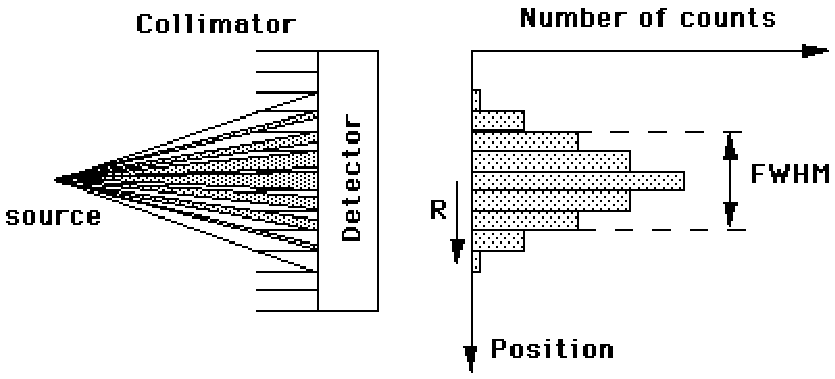
\includegraphics[width=0.5\textwidth]{figs/fig_collimatorpsf.pdf}
\caption{\label{fig:collimatorpsf} \emph{Point spread function of
          the collimator. The number of detected photons at a point in the
          detector decreases linearly with the distance $r$ to the central
          point.}}
\end{figure}

In the calculations above, the thickness of the septa has been
ignored. In reality, the septa have to be thick enough to stop the
photons hitting them. Septa are made from high-Z materials, like lead
or tungsten, to maximize the photon attenuation. High resolution
collimators are optimized for imaging with \textsuperscript{99m}Tc: the septa are
relatively thin, and $a/T$ is small, resulting in high resolution but
not so high sensitivity. High sensitivity collimators have a larger
$a/T$, producing poorer resolution. High energy collimators are
designed for isotopes emitting high energy photons, such as $^{131}$I
(see table \ref{tab:rntisotopes}). They have thicker septa to
minimize the number of photons penetrating them. To account for
the septa thickness, equation (\ref{eq:collim:sens}) can be extended
to
\begin{equation}
  \mbox{sens} =  \frac{1}{12} \left( \frac{a}{T} \right)^2
                 \;\frac{a^2}{(a+s)^2}
\end{equation}
where $a$ is the distance between neighboring septa and $s$ is the septa
thickness. Using thicker septa while keeping the resolution reduces
the collimator sensitivity.


\subsection{Electronic and mechanical collimation in the PET camera} \label{sec:petcollim}
%===================================================================
\subsubsection{Electronic collimation: coincidence detection}
%------------------------------------
During positron annihilation, two photons are emitted in opposite
directions. If both are detected, we know that the annihilation occurred
somewhere on the line connecting the two detectors. So in contrast to SPECT,
no mechanical collimator is needed. However, we need fast electronics, since
the only way to test if two detected photons could belong together, is by
checking if they have been emitted simultaneously.

We first consider a single detector pair as shown in figure
\ref{fig:petdetectorpair}, and study its characteristics by computing its
response to a point source. The detector has a square surface of size $d$, and
the distance between the detectors is $2R$. We choose the origin in the point of
symmetry, and see how the response changes if we change the position of the
point source. Keep in mind that an event is only valid if both photons of the
photon pair are detected.
%
\begin{figure}[tb]
\centering
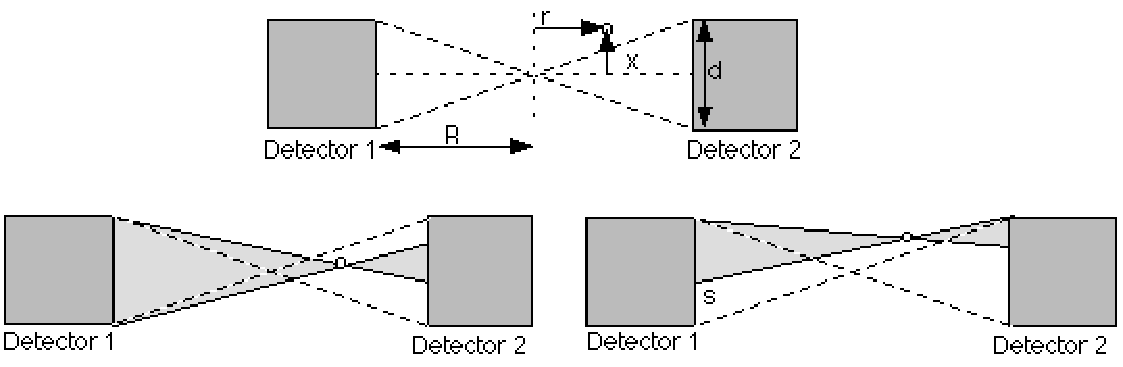
\includegraphics[width=0.9\textwidth]{figs/fig_petdetectorpair.pdf}
\caption{\label{fig:petdetectorpair} \emph{A point source positioned in the
field of view of a pair of detectors}}.
\end{figure}

Assume that the point source is moved along the $r$-axis: $x = 0$. Then the
limiting detector is the far one: if one photon reaches the far detector, the
other photon will surely reach the other detector. The number of detected
photon pairs is proportional to the solid angle occupied by the two detectors:
\begin{equation}
  \mbox{PSF}(x=0, r) = \frac{2 d^2}{4 \pi (R+r)^2} = \frac{d^2}{2 \pi (R+r)^2}
\end{equation}
This is an approximation: we assume that the far detector surface coincides
with the surface of a sphere of radius $R+r$. It does not, because it is flat.
However, because $d$ is very small compared to $R$, the approximation is very
good.

We now move the point source vertically over a distance $x$. As long as the
point is between the dashed lines in figure \ref{fig:petdetectorpair}, nothing
changes (that is, if we ignore the small decrease in solid angle due to the
fact that the detector surface is now slightly tilted when viewed from the
point source). However, when the point crosses the dashed line, the far
detector is no longer fully irradiated. A part of the detector surface no
longer contributes: if a photon reaches that part, the other photon will miss
the other detector. The height $s$ is computed from simple geometry (figure
\ref{fig:petdetectorpair}):
\begin{equation}
  s(x) = \left( |x| - \frac{d |r|}{2 R} \right) \frac{2R}{R-|r|}
\end{equation}
The first factor is the distance between the point and the dashed line, the
second factor is the magnification due to projection of that distance to the
far detector. This equation is only valid when $d r / (2R) \leq x \leq
d/2$. Otherwise, $s = 0$ if $x$ is smaller than $dr/(2R)$, and $s = d$ if $x$
is larger. In the center, $r = 0$ and we have simply that $s(x) = 2 |x|$.
Knowing the active detector area, we can immediately compute the
corresponding solid angle to obtain the detector pair sensitivity as a
function of the point source position (which can be regarded as a PSF):
\begin{equation}
 \mbox{PSF}(x, r) = \frac{(d - s(x)) d}{2 \pi (R+|r|)^2}
\end{equation}
We can move the point also in the third dimension, which we will call $y$. The
effect is identical to that of changing $x$, so we obtain:
\begin{equation}
 \mbox{PSF}(x, y, r) = \frac{(d - s(x)) (d - s(y))}{2 \pi (R+|r|)^2}
\end{equation}

From these equations it follows that the PSF is triangular in the center,
rectangular close to the detectors and trapezoidal in between.  Introducing
that third dimension, we obtain for the PSF in the center and close to the
detector respectively:
\begin{eqnarray}
  \mbox{PSF}(x, y, 0) & = & \frac{(d - 2|x|)(d - 2 |y|)}{2 \pi R^2}\\
  \mbox{PSF}(x, y, R) & = & \frac{d^2}{8 \pi R^2}
\end{eqnarray}
We can compute the average sensitivity within the field of view by integrating
the PSF over the detector area $x \in [-d/2, d/2], y \in [-d/2,
d/2]$ and divide by $d^2$. It is simple to verify that in both cases we obtain:
\begin{equation}
  \mbox{sens} = \frac{d^2}{8 \pi R^2} \label{eq:pet_totsens}
\end{equation}
showing that sensitivity is independent of position in the detection plane, if
the object is large compared to $d$.

Finally, we can estimate the sensitivity of a complete PET system consisting
of a detector ring with thickness $d$ and radius $R$, assuming that we have a
positron emitting source near the center of the ring. We assume that the ring
is in the $(y,r)$-plane, so the $x$-axis is the symmetry axis of the detector
ring.  One approach is to divide the detector area by the area of a sphere
with radius $R$, as we have done before. This yields:
\begin{equation}
  \mbox{PETsens}_{x=0} = \frac{2 \pi d R}{ 4 \pi R^2} = \frac{d}{2R}
\end{equation}
This is the maximum sensitivity, obtained for $x = 0$. The average over $ =
-d/2 \ldots d/2$ is half that value, since in the center of the PET, the
sensitivity varies linearly between the maximum and zero:
\begin{equation}
  \mbox{PETsens} = \frac{d}{4R}. \label{eq:petsens}
\end{equation}

\subsubsection{Resolution of coincidence detection}
%------------------------------------
Until now, we have always assumed that annihilation takes place very close to
the emission point, and that the photons are emitted in exactly opposite
directions. In reality, there are small deviations, which limit the
theoretical resolution of PET. 

\begin{table}
\caption{Maximum and mean kinetic energy (k.e.), maximum and mean path length
of the positron for the most common PET isotopes.}
\label{tab:positron_length}
\begin{center}
\begin{tabular}{|c|c|c|c|c|}
\hline
Isotope   & Max k.e. [MeV] & mean k.e. [MeV] & Max path [mm] & Mean path [mm]\\
\hline
$^{11}$C  & 0.96 & 0.39 & 3.9    & 1.1 \\
$^{13}$N  & 1.19 & 0.49 & 5.1    & 1.5 \\
$^{15}$O  & 1.72 & 0.73 & 8.0    & 2.5 \\
$^{18}$F  & 0.64 & 0.25 & 2.4    & 0.6 \\
$^{68}$Ga & 1.90 & 0.85 & 8.9    & 2.9 \\
$^{82}$Rb & 3.35 & 1.47 & 17     & 5.9 \\
\hline
\end{tabular}
\end{center}
\end{table}

As shown in table \ref{tab:positron_length}, the path depends on the
kinetic energy of the positron. The positron can only annihilate if
its kinetic energy is sufficiently low, so if it is emitted at high
speed, it will travel ``far'' (up to a few mm). During its trajectory,
it dissipates its energy in collisions with surrounding electrons. The
mean path length (positron range) of $^{18}$F is small and has a very
limited effect on the spatial resolution. For some other isotopes,
like $^{68}$Ga and $^{82}$Rb, the positron range is several mm.

Momentum is preserved during annihilation, so the momentum of both photons
must equal the momentum of the positron and the electron. This momentum is
usually not zero, so the photons cannot be emitted in exactly opposite
directions (the momentum of a photon is a vector with amplitude $h/\lambda$
and pointing in the direction of propagation). As shown in figure
\ref{fig:positron_error}, there is a deviation of about 0.5\textdegree, which
corresponds to a 2.0 mm offset for a detector ring with 80 cm diameter.
%
\begin{figure}[tb]
\centering
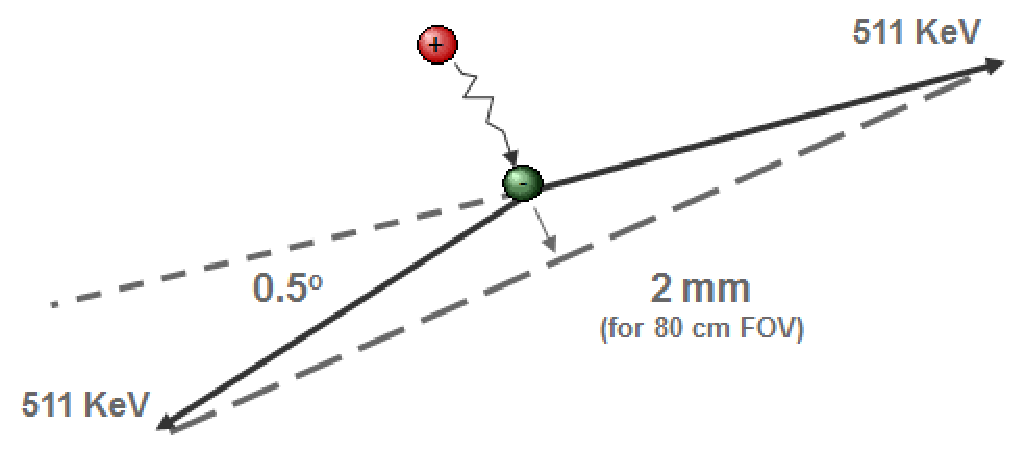
\includegraphics[width=0.5\textwidth]{figs/fig_positron_error.pdf}
\caption{\label{fig:positron_error} \emph{The distance traveled by the
positron and the deviation from 180 degrees in the angle between the photon
paths limit the best achievable resolution in PET}}.
\end{figure}


\begin{figure}[tb]
\centering
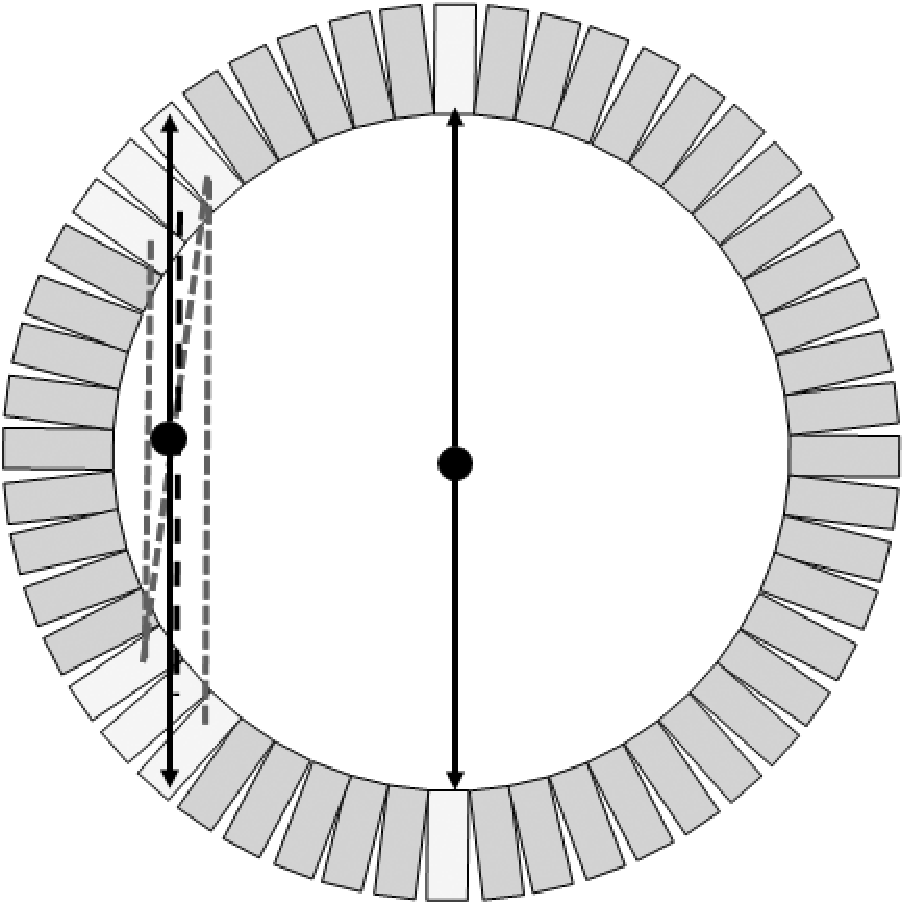
\includegraphics[width=0.3\textwidth]{figs/fig_doi.pdf}
\caption{\label{fig:doi} \emph{Resolution loss as a result of
    uncertainty about the depth of interaction}}.
\end{figure}
%
The resolution is further degraded by the unknown ``depth of
interaction'' of the photon inside the crystal. As shown in figure
\ref{fig:doi}, photons emitted near the edge of the field of view
might traverse one crystal to scintillate only in the next
one. Because we don't know where in the crystal the scintillation took
place, we always have to assign a fixed depth of interaction to the
event. The mispositioning of these events causes a loss of resolution
that increases with the distance from the center. PET systems have
been designed and built that can measure the depth of interaction to
reduce this loss of resolution.


\subsubsection{Mechanical collimation: inter-plane septa} \label{sec:septa}
%------------------------------------
In the previous section we have seen why a PET-camera does not need a
collimator. We also know that the PET-camera can only measure photon pairs
originating somewhere within the detection plane. However, photons coming from
radioactivity outside that plane could also reach the detectors, and produce
undesired scintillations, which provide no information, or even worse, wrong
information. Therefore, it is useful to shield the detector ring against
photons coming from outside the field of view. This is done with so-called
septa, as shown in figure \ref{fig:pet_septa}. The septa provide some
collimation in the direction perpendicular to the detection plane, but there is
no collimation within the plane. The septa reduce the number of single
photons, scattered photons, random coincidences and triple (or more)
coincidences.

%
\begin{figure}[tb]
\centering
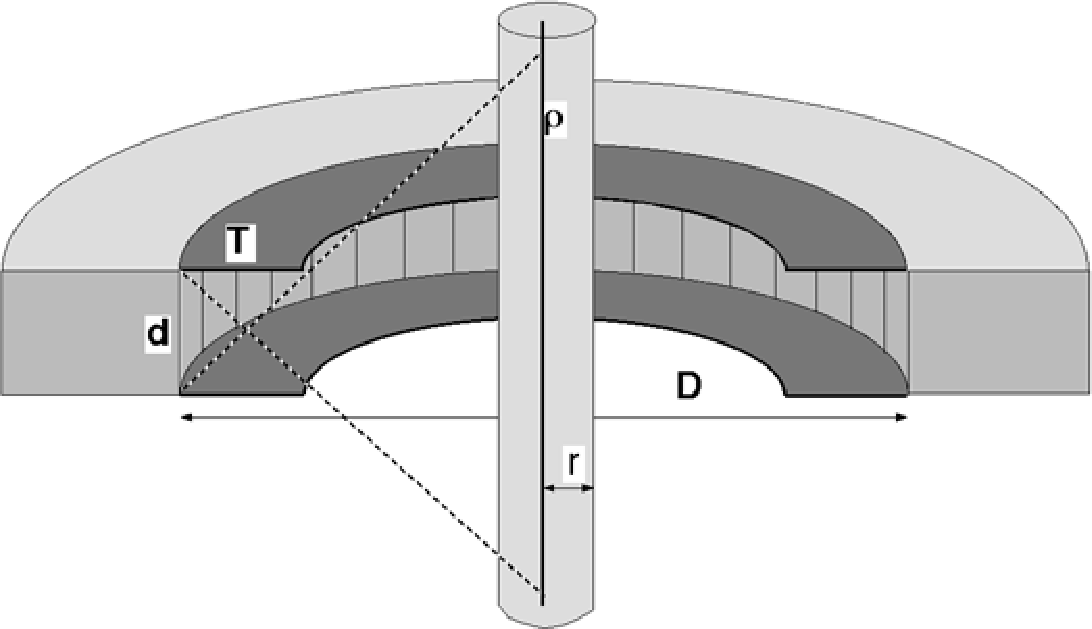
\includegraphics[width=0.5\textwidth]{figs/fig_pet_septa.pdf}
\caption{\label{fig:pet_septa} \emph{A PET ring detector (cut in half) with a
cylindrical homogeneous object, containing a radioactive wire near the
symmetry axis}}.
\end{figure}

Before these events are described, we have to better define what is meant with
a coincidence. Two photons are detected {\em simultaneously} if the difference
in detection times is lower than a predefined threshold, the ``time window''
of the PET-system. The time window cannot be arbitrarily short for the
following reasons:
\begin{itemize}
  \item The time resolution of the electronics is limited: electricity is
        never faster than light, and it is delayed in every electronical
        component.  Of course, we do not want to reject true coincidences
        because of errors in timing computation.
  \item The diameter of the PET-camera is typically about 1 m for a
        whole body system, and about half that for a brain
        system. Light travels about 1 m in 3 ns. Consequently, the
        time window should not be below 3 ns for a 1 m diameter
        system.
\end{itemize}
For these reasons, current systems use a time window of about 5 to 10
ns. Recently, PET systems have been built with a time resolution
better than 1 ns. With those systems, one can measure the difference
in arrival time between the two photons and deduce some position
information from it. This will be discussed in section \ref{sec:TOF}.

Figure \ref{fig:pet_random_enzo} shows the difference between a true
coincidence, which provides valuable information, and several other events
which are disturbing or even misleading. A single event provides no
information and is harmless. But if two single events are simultaneous (random
coincidence), they are indistinguishable from a true coincidence. If one (or
both) of the photons is scattered, the coincidence provides wrong information:
the decaying atom is not located on the line connecting the two
detectors. Finally, a single event may be simultaneous with a true
coincidence. Since there is no way to find out which of the three photons is
the single one, the entire event is ignored and information is lost.

\begin{figure}[tb]
\centering
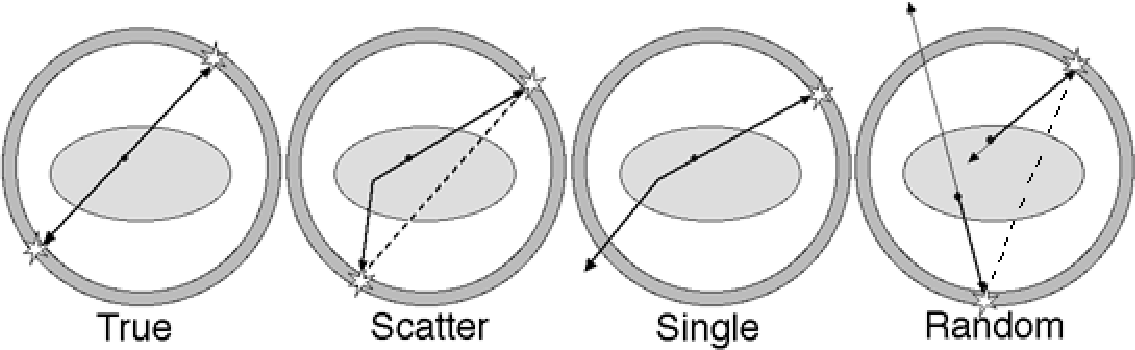
\includegraphics[width=0.9\textwidth]{figs/fig_pet_random_enzo.pdf}
\caption{\label{fig:pet_random_enzo} \emph{True coincidence, scattered
coincidence, single event, random coincidence}}.
\end{figure}

To see how the septa dimensions influence the relative contribution of the
various possible events, some simple computations can be carried out using the
geometry shown in figure \ref{fig:pet_septa}. Assume that we have a
cylindrical object in the PET-camera. In the center of the cylinder, there is
a radioactive wire, with activity $\rho$ per unit length. The cylinder has
radius $r$ and attenuation coefficient $\mu$. This object represents an
idealized patient: there is activity, attenuation and Compton scatter in the
attenuating object as in a patient; the unrealistic choice of dimensions makes
the computations easier. The PET-camera diameter is $D$, the detector size is
$d$ and the septa have length $T$. The duration of the time window is
$\tau$. Finally, we assume that the detector efficiency is $\epsilon$, which
means that if a photon reaches the detector, it has a chance of $\epsilon$ to
produce a valid scintillation, and a chance of $1 - \epsilon$ to remain
undetected.\\[2mm]

To compute the number of {\bf true coincidences} per unit of time, we must
keep in mind that both photons must be detected, but that their paths are not
independent. To take into account the influence of the time window, it helps
to consider first a short time interval equal to the time window $\tau$. After
that, we convert the result to counts per unit of time by dividing by
$\tau$. Why we do this will become clear when dealing with randoms. We proceed
as follows:
\begin{itemize}
%
\item The activity in the field of view is $\rho d$. 
%
\item Both photons can be attenuated, the attenuated activity is $\rho d a^2$,
with $a = \exp(-\mu r)$.
%
\item As we have derived above (see eq (\ref{eq:petsens})), the
geometrical sensitivity is $d/(2D)$.
%
\item Both photons must be detected if they hit the detectors, so the
effective sensitivity is $\epsilon^2 d / (2D)$.
%
\item The probability that a photon will be seen is proportional to the
      scan time $\tau$.
%
\item To compute the number of counts per time unit, we multiply with $1/\tau$.
\end{itemize}
We only care about the influence of the design parameters, so we ignore all
constants. This leads to:
\begin{equation}
  \mbox{trues} \sim \rho a^2 \epsilon^2 \frac{d^2}{D} \label{eq:pet_trues}
\end{equation}

For {\bf scatters} the situation is very similar, except for two
issues: (1) the probability for a scatter event to occur depends on the
attenuating material and (2), the combined photon path is not a
straight line but a broken one.

Consider a source with activity $\lambda$ emitting photons at $x = 0$
along the $x$-axis, in a material met linear attenuation coefficient
$\mu$ that covers the interval $x \in [-r, r]$. Then the probability
of a photon arriving at $x$ is proportional to $\lambda e^{- \mu x}$,
and the probability that it scatters there is proportional to $\lambda
e^{- \mu x} \mu \; dx$. The probability that this scattered photon will
not be attenuated is determined by how much material it is propagating
through, and can be roughly estimated as $e^{\mu(r-x)}$. To obtain all
scattered photons leaving the object we integrate this from the source
position to the boundary of the material: 
\begin{equation}
  \lambda \int_0^r e^{-\mu x} \mu \; e^{-\mu(r - x)} dx \;\;\;
  = \;\; \lambda e^{-\mu r} \mu r \;\;
  = \;\; \lambda a \mu r,
\end{equation}
where the last equation is obtained by setting $e^{-\mu r} = a$.

The other issue is that the combined photon path is a broken
line. This has two consequences. First, the field of view is larger
than for the trues. Second, the path of the second photon is (nearly)
independent of that of the first one.

We will assume that only one of the photons undergoes a single Compton scatter
event, so the path contains only a single break point. The corresponding field
of view is indicated with the dashed line in figure \ref{fig:pet_septa}. The
length of the wire in the field of view is then $d (D-T) / T$, but since $T$ is
much smaller than $D$ we approximate it as $d D/T$.

Each of the photons goes its own way. This will only lead to detection if both
happen to end up on a detector and are detected. For each of them, that
probability is proportional to $\epsilon d / D$, so for the pair the detection
probability is $(\epsilon d / D)^2$. For the trues this factor was not
squared, because detection of one photon guarantees detection of the other!

Attenuation of scattered photons is complex, since they have lower energy and
travel along oblique lines. However, if we assume that the septa are not too
short and that the energy resolution is not too bad, we can ignore all that
without making too dramatic an error. (We only want to see the major
dependencies, so we can live with moderately dramatic errors.)
Consequently, we have for the scatters count rate
\begin{equation}
  \mbox{scatters} \;\;\sim\;\; \rho d \frac{D}{T} \; \mu r \; a^2
     \; \left( \frac{\epsilon d}{D} \right)^2
  \;\;=\;\;  \rho \mu r a^2 \epsilon^2 \frac{d^3}{DT}
       \label{eq:pet_scatters}
\end{equation}

A {\bf single}, non-scattered photon travels along a straight line, so the
singles field of view is the same as that of the scatters, and the
contributing activity is $\rho d D / T$. The attenuation is $a$. The effective
sensitivity is proportional to $\epsilon d / D$. The number of singles in a
time $\tau$ is proportional to $\tau$. Finally, we divide by $\tau$ to obtain
the number of single events per unit of time. This yields:
\begin{equation}
  \mbox{singles} \sim \rho a \epsilon \frac{d^2}{T} \label{eq:pet_singles}
\end{equation}

A {\bf random coincidence} consists of two singles, arriving {\em
simultaneously}. So if we study a short time interval $\tau$ equal to the time
window, we must simply multiply the probabilities of the two singles, since
they are entirely independent of each other. Afterwards, we multiply with
$1/\tau$ to compute the number of counts per time unit. So we obtain:
\begin{equation}
  \mbox{randoms} \sim \rho^2 a^2 \epsilon^2 \frac{d^4}{T^2} \tau
      \label{eq:pet_randoms}
\end{equation}

Similarly, we can compute the probability of a ``{\bf triple coincidence}'',
resulting from simultaneous detection of a true coincidence and a single
event. This produces:
\begin{equation}
  \mbox{true + single} \sim \rho^2 a^3 \epsilon^3 \frac{d^4}{TD} \tau
\end{equation}

As you can see, the trues count rate is not affected by either $\tau$
nor $T$, in contrast to the unwanted events. Consequently, we want
$\tau$ to be as short as possible to reduce the randoms and triples
count rate. We have seen that for current systems this is about 10 ns
or even less. Similarly, we want $T$ to be as large as possible to
reduce all unwanted events. Obviously, we need to leave some room for
the patient.


\subsubsection{2D and 3D PET} \label{sec:2D3DPET}
%------------------------------------
In the previous paragraphs we have studied a single ring of PET
detectors, and we have shown that shielding the detectors with septa
reduces the scatter and random coincidence rate, without affecting the
true coincidence rate. In current clinical systems, multiple rings are
combined in a single device, as shown in figure \ref{fig:jnpet}. In
the past, many of these systems could be operated in two modes.  In
2D-mode, the rings are separated by septa. In 3D-mode, the septa are
retracted, only the shielding at the edges of the axial field of view
remain. Current PET systems have no septa between the detector rings,
they are always operated in 3D mode.

\begin{figure}[tb]
\centering
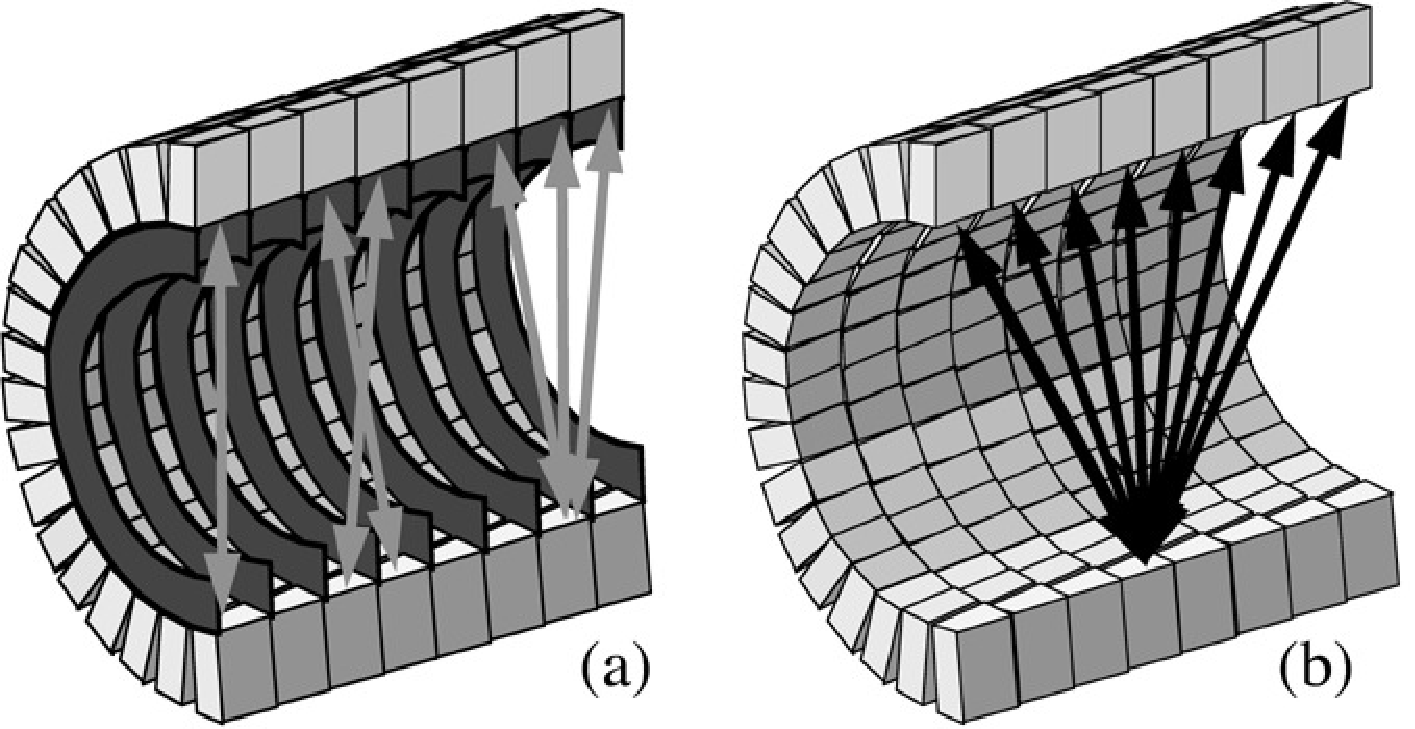
\includegraphics[width=0.5\textwidth]{figs/fig_jnpet.pdf}
\caption{\label{fig:jnpet} \emph{Positron emission tomograph (cut in
half). When septa are in the field of view (a), the camera can be regarded as
a series of separate 2D systems. Coincidences along oblique projection lines
between neighboring rings can be treated as parallel projection lines from an
intermediate plane. This doubles axial sampling: 15 planes are reconstructed
from 8 rings. Retracting the septa (b), increases the number of projection
lines and hence the sensitivity of the system, but fully 3D reconstruction is
required.}}
\end{figure}

In 2D mode, there are two types of planes: direct planes, located in the
center of the ring, and cross-planes, located between two neighboring
rings. The direct planes correspond to what we have seen above for a single
ring system. A photon pair belongs to a cross plane if one photon is detected
in ring $i$ and the other one in ring $i+1$. The small inclination of the
projection line can be ignored, and such coincidences are processed as if they
were acquired by an imaginary detector ring located at $i + 0.5$. This
improves axial sampling. It turns out that the cross-planes are in fact
superior to the direct planes: near the center the axial resolution is
slightly better because of the shadow cast by the septa on the contributing
detectors, and the sensitivity is nearly twice that of direct planes because
of the larger solid angle.

According to the Nyquist criterion, the sampling distance should not be longer
than half the period of the highest special frequency component in the
acquired signal (you need at least two samples per period to represent a sine
correctly). Without the cross-planes, the criterion would be violated. So the
cross-planes are not only useful to increase sensitivity, the are needed to
avoid aliasing as well.\\[2mm]

In 3D mode, the septa are retracted, except for the first and last one. The
detection is no longer restricted to parallel planes, photon pairs traveling
along oblique lines are now accepted as well. In chapter
\ref{ch:image_formation} we will see that this has a strong impact on image
reconstruction.

This has no effect on spatial resolution, since that is determined by
the detector size. But the impact on sensitivity is very high. In fact,
we have already computed all the sensitivities in section
\ref{sec:septa}. Those expressions are still valid for 3D PET, if we
replace $d$ (the distance between the septa) with $Nd$, where $N$ is
the number of neighboring detector rings. To see the improvement for
3D mode, you have to compare to a concatenation of $N$ independent
detector rings (2D mode), which are $N$ times more sensitive than a
single ring (at least if we wish to scan an axial range larger than
that seen by a single ring). So you can see that the sensitivity for
trues increases with a factor of $N$ when going from 2D to
3D. However, scatters increase with $N^2$ and randoms even with
$N^3$. Because the 3D PET is more sensitive, we can decrease the
injected dose with a factor of $N$ (preserving the count rate). If we
do that, randoms will only increase with $N^2$. Consequently, the
price we pay for increased sensitivity is an even larger increase of
disturbing events. So scatter and randoms correction will be more
important in 3D PET than in 2D PET. It turns out that scatter in
particular poses problems: it was usually ignored in 2D PET, but this
is no longer acceptable in 3D PET. Various scatter correction
algorithms for 3D PET have been proposed in the literature, the one
mostly used is described below (\ref{sec:petscatcor}).

\section{Partial volume effect} \label{sec:pv}
%%%%%%%%%%%%%%%%%%%%%%%%%%%%%%%%%%%%%%%%%
\begin{figure}[tb]
\centering
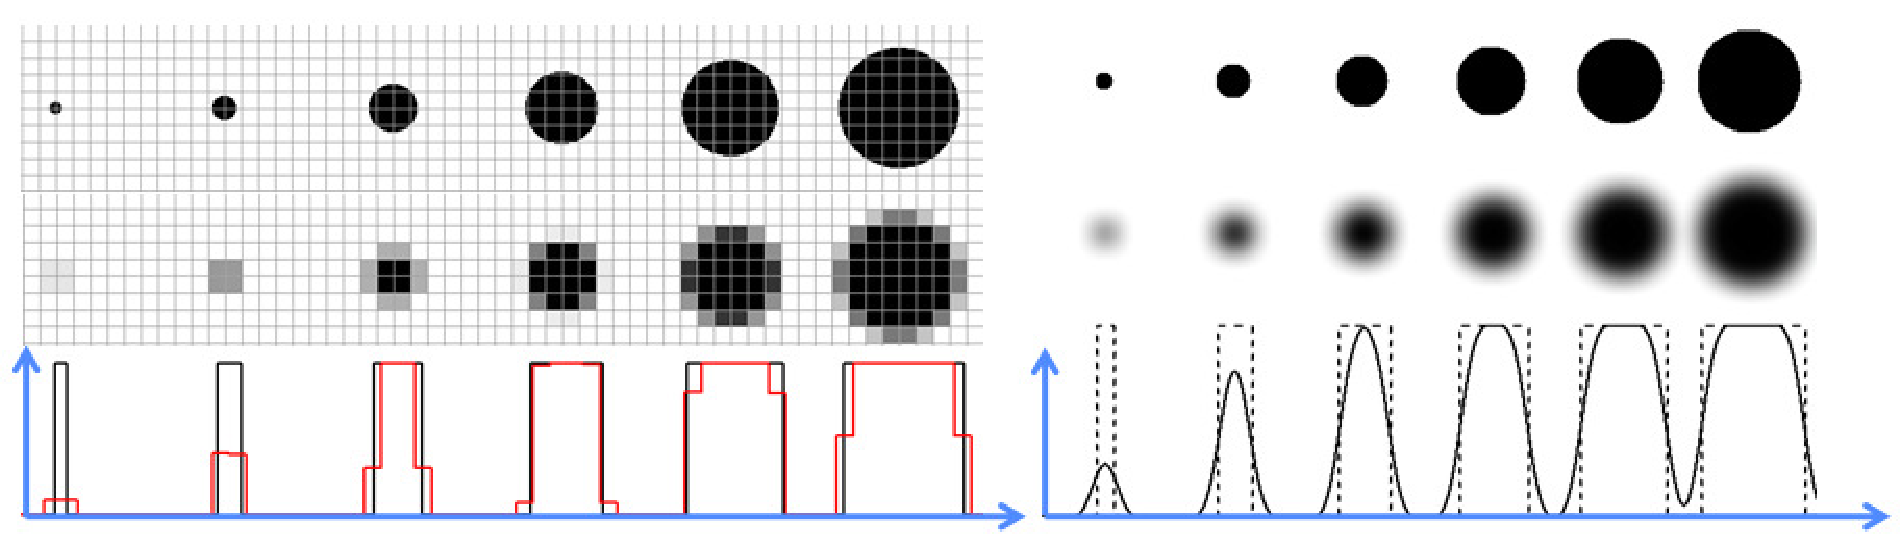
\includegraphics[width=0.9\textwidth]{figs/fig_pv.pdf}
\caption{\label{fig:pv} \emph{The partial volume effect caused by the
finite pixel size (left), and by the finite system PSF (right). The
first row shows the true objects, the second row illustrates the
partial volume effect due to pixels and PSF, and the last row compares
horizontal profiles to the true objects and the images.  Objects that
are small compared to the pixel size and/or the PSF are poorly
represented.}}
\end{figure}
%
As explained above, resolution is not the strongest point of nuclear
medicine. Other medical imaging systems (CT, MR, ultrasound) have a
much better resolution. One often uses the term {\em partial volume
effect} to refer to problems caused by poor resolution. The idea is
that if an object only fills part of a pixel, the pixel contains two
things: object and background. Because the pixel has only one value,
it does not give a reliable representation of either. Figure
\ref{fig:pv} illustrates this for a disk imaged with some imaging
system. If the object is large compared to the pixels of the image,
then the image gives a good representation of the object. However,
small objects are poorly represented. As can be seen in the profiles,
the maximum value in the image is much smaller than the true maximum
intensity of the object. The obvious remedy is to use sufficiently
small pixels.

However, if the pixels are small, the imaging performance is limited
by the system point spread function, as illustrated in the second
panel of figure \ref{fig:pv}. The image can be regarded as a
convolution of the true intensities with the PSF. The effect is very
similar as that of the big pixels, one could say that the object only
partially fills the PSF. Again, the maximum intensity of small objects
is severely underestimated, and their size is overestimated.

Consequently, nuclear medicine imaging systems tend to underestimate
the maximum intensity and overestimate the size of small objects. The
{\em recovery coefficient} is the ratio of the estimated and true
maximum. The so-called {\em spill over} is the amount of apparent
activity showing up outside the true object boundaries due to the
blurring.

\section{Compton scatter correction} \label{sec:scatter}
%%%%%%%%%%%%%%%%%%%%%%%%%%%%%%%%%%%%%%%%%
% Scatter in SPECT, evt meerdere energieen.
% Pile-up
%----
\subsection{Gamma camera} \label{sec:spectscatcor}
%------------------------
Compton scatter causes photons to be deviated from their original trajectory,
and to propagate with reduced energy along a new path. Consequently, photons
with reduced energy can reach the detector via a broken line. Such photons are
harmful: they provide no useful information and produce an unwanted
inhomogeneous background in the acquired images (fig
\ref{fig:scatter_gammacamera}).

\begin{figure}[tb]
\centering
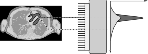
\includegraphics[width=0.5\textwidth]{figs/fig_scatter_gammacamera.pdf}
\caption{\label{fig:scatter_gammacamera} \emph{Compton scatter allows
photons to reach the camera via a broken line. These photons produce a smooth
background in the acquired projection data.}}
\end{figure}

We have seen in section \ref{sec:compton_scatter} that the photon loses more
energy for larger scatter angles. The gamma camera (or the PET camera) measures
the energy of the photon, so it can reject the photon if its energy is low.

However, if the energy loss during Compton scatter is smaller than or
comparable to the energy resolution of the gamma camera, then it may
survive the energy test and get accepted by the camera. Figure
\ref{fig:scatter_spectrum} shows the energy spectrum as measured by
the gamma camera. A Monte Carlo simulation was carried out as well,
and the resulting spectrum is very similar to the measured one. The
simulation allows to compute the contribution of unscattered (or
primary) photons, photons that scattered once and photons that
suffered multiple scatter events. If the energy resolution were
perfect, the primary photon peak would be infinitely narrow and all
scattered photons could be rejected. But with a realistic energy
resolution the spectra overlap, and acceptance of scattered photons is
unavoidable.

\begin{figure}[tb]
\centering
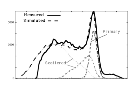
\includegraphics[width=0.5\textwidth]{figs/fig_scatter_spectrum.pdf}
\caption{\label{fig:scatter_spectrum} \emph{The energy spectrum measured by
the gamma camera, with a simulation in overlay. The simulation allows to
compute the spectrum of non-scattered (primary) photons, single scatters and
multiple scatters. The true primary spectrum is very narrow, the measured one
is widened by the limited energy resolution.}}
\end{figure}

Figure \ref{fig:scatter_spectrum} shows a deviation between simulation and
measurement for high energies. In the measurement it happens that two photons
arrive simultaneously. If that occurs, the gamma camera adds their energies
and averages their position, producing a mispositioned count with high
energy. Such photons must be rejected as well. The simulator assumed
that each photon was measured independently. The simulator deviates also at
low energies from the measured spectrum, because the camera has not recorded
these low-energy photons.

To reject as much as possible the unwanted photons, a narrow energy
window is centered around the tracer energy peak, and all photons with
energy outside that window are rejected. Current gamma cameras can use
multiple energy windows simultaneously. That allows us to administer
two or more different tracers to the patient at the same time, if we
make sure that each tracer emits photons at a different energy. The
gamma camera separates the photons based on their energy and produces
a different image for each tracer. For example, $^{201}$Tl emits
photons of about 70 keV (with a frequency of 0.70 per desintegration)
and 80 keV (0.27 per desintegration), while \textsuperscript{99m}Tc\ emits photons
of about 140 keV (0.9 per desintegration). $^{201}$Tl labeled thallium
chloride can be used as a tracer for myocardial blood perfusion. There
are also \textsuperscript{99m}Tc\ labeled perfusion tracers. These tracers are
trapped in proportion to perfusion, and their distribution depends
mostly on the perfusion at the time of injection.  Protocols have been
used to measure simultaneously or sequentially the perfusion of the
heart under different conditions. In one such protocol, $^{201}$Tl is
injected at rest, and a single energy scan is made. Then the patient
exercises to induce the stress condition, the \textsuperscript{99m}Tc\ tracer is
injected at maximum excercise, and after 30 to 60 min, a scan with
energy window at 140 keV is made. If the same tracer were used twice,
the image of the stress perfusion would be contaminated by the tracer
contribution injected previously at rest.

Since not all unwanted photons can be rejected, an additional correction may
be required. Figure \ref{fig:TEW_scatter} shows a typical correction method
based on three energy windows. Window C1 is the window centered on the energy
of the primary photons. If we assume that the spectrum of the unwanted photons
varies approximately linearly over the window C1, then we can estimate that
spectrum by measuring in two additional windows C2 (just below C1) and C3
(just above C1). If all windows had the same size, then the number of unwanted
photons in C1 could be estimated as (counts in C2 + counts in C3) / 2. Usually
C2 and C3 are chosen narrower than C1, so the correction must be weighted
accordingly. In the example of figure \ref{fig:TEW_scatter} there are very few
counts in C3. However, if we would use a second tracer with higher energy,
then C3 would receive scattered photons from that tracer.

\begin{figure}[tb]
\centering
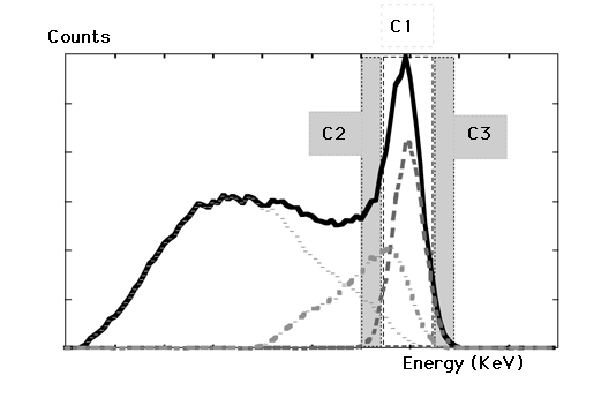
\includegraphics[width=0.5\textwidth]{figs/fig_TEW_scatter.pdf}
\caption{\label{fig:TEW_scatter} \emph{Triple energy window correction. The
amount of scattered photons accepted in window C1 is estimated as a fraction
of the counts in windows C2 and C3.}}
\end{figure}

\subsection{PET camera} \label{sec:petscatcor}
%----------------------
Just like the gamma camera, the PET camera uses a primary energy
window to reject photons with an energy that is clearly different from
511 keV. However, the energy resolution of current PET systems is
poorer than that of the gamma camera (15$\ldots$20\%). Unfortunately,
with poorer energy resolution, scatter correction based on an
additional energy window is less accurate. The reason is that the
center of the scatter window C2 has to be shifted farther away from
the primary energy peak, here 511 keV. Hence, the photons in that
window have lost more energy, implying that they have been scattered
over larger angles. Consequently, they are a poorer estimate of the
scatter inside the primary window, which has been scattered over
smaller angles.

For that reason, PET systems use a different approach to scatter
correction. As will be seen in chapter \ref{ch:trans}, PET scanners
are capable of measuring the attenuation coefficients of the patient
body. This can be used to calculate an estimate of the Compton scatter
contribution, if an estimate of the tracer distribution is available,
and if the characteristics of the PET system are known. Such
computations are done with Monte Carlo simulation. The simulator
software ``emits'' photons in a similar way as nature does: more
photons are emitted where more activity is present, and the photons
are emitted in random (pseudo-random in the software) directions. In a
similar way, photon-electron interactions are simulated, and each
photon is followed until it is detected or lost for detection
(e.g. because it flies in the wrong direction). This must be repeated
for a sufficient amount of photons, in order to generate a reasonable
estimate of the scatter contribution. Various clever tricks have been
invented to accelerate the computations, such that the whole procedure
can be done in a few minutes.

In practice, the method works as follows. First, a reconstruction of
the tracer uptake without scatter correction is computed. Based on
this tracer distribution and on the attenuation image of the patient,
the scatter contribution to the measured data is estimated with the
simulation software. This scatter contribution can then be subtracted
to produce a better reconstruction of the tracer distribution. This
procedure can be iterated to refine the scatter estimate.

\begin{figure}[tb]
\centering
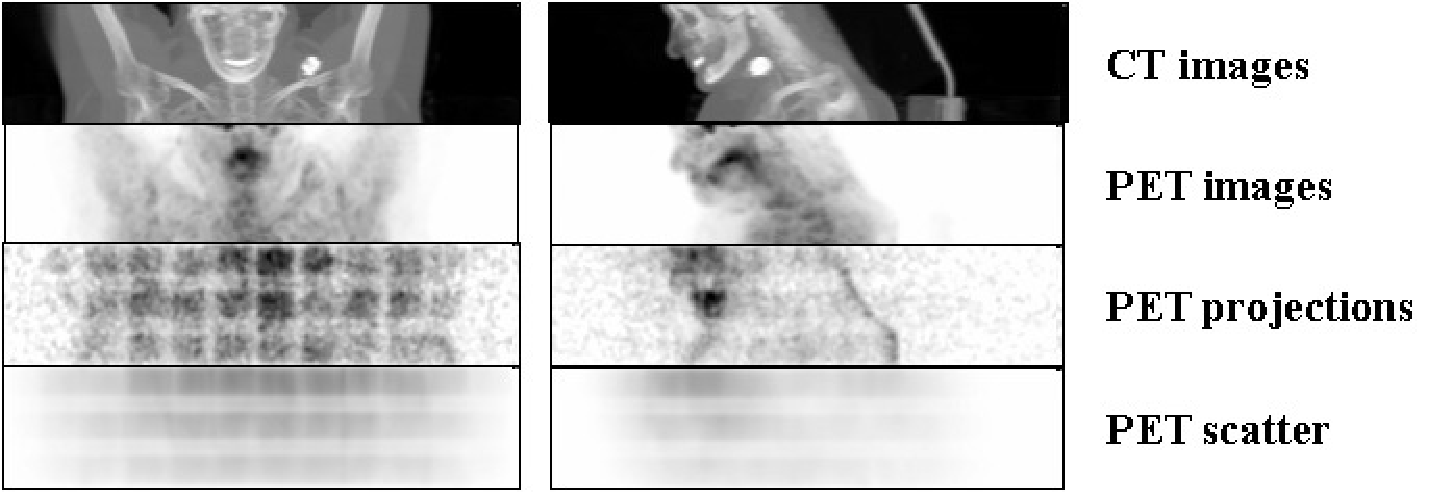
\includegraphics[width=0.9\textwidth]{figs/fig_pet_scatter.pdf}
\caption{\label{fig:petscatter} \emph{CT and PET images (obtained by
    maximum intensity projection), and the corresponding raw PET
    projection data with their estimated scatter contribution. Data
    were acquired with a Biograph 16 PET/CT system (Siemens). The
    regular pattern in the raw data is due to sensitivity differences
    between different detector pairs (see also fig \ref{fig:pet_norm}).}}
\end{figure}

Figure \ref{fig:petscatter} gives an example of the original raw PET
data from a 3D PET scan (slightly smoothed so you would see
something), together with the corresponding estimated scatter
contribution (using the same gray scales). Maximum intensity
projections of the CT and PET images are shown as well. The regular
pattern in the raw PET data is due to position dependent sensitivities
of the detector pairs (see also fig. \ref{fig:pet_norm}). The scatter
distribution is smooth, and its amplitude is significant.


\section{Other corrections} \label{sec:corrections}
%%%%%%%%%%%%%%%%%%%%%%%%%%%%%%%%%%
% Typische gamma camera
% Typische PET camera
% Linearity
% Energy
% Uniformity
% Dead time
%---
Currently, most gamma camera designs are based on a single crystal detector
as shown in figure \ref{fig:gammacamera}. To increase the sensitivity, a
single gamma camera may have two or three detector heads, enabling
simultaneous acquisition of two or three views along different angles
simultaneously. Because the detector head represents a significant portion of
the cost of the gamma camera, the price increases rapidly with the number of
detector heads.

Most PET systems have a multi-crystal design, they consist of multiple rings
(fig \ref{fig:jnpet}) of small detectors. The detectors are usually arranged
in modules (fig \ref{fig:multicrystal}) to reduce the number of PMT's.

The performance of the PMT's is not ideal for our purposes, and in addition
they show small individual differences in their characteristics. In current
gamma cameras and PET cameras the PMT-gain is computer controlled and
procedures are available for automated PMT-tuning. But even after tuning,
small differences in characteristics are still present.  As a result, some
corrections are required to ensure that the acquired information is reliable.

\begin{figure}[tb]
\centering
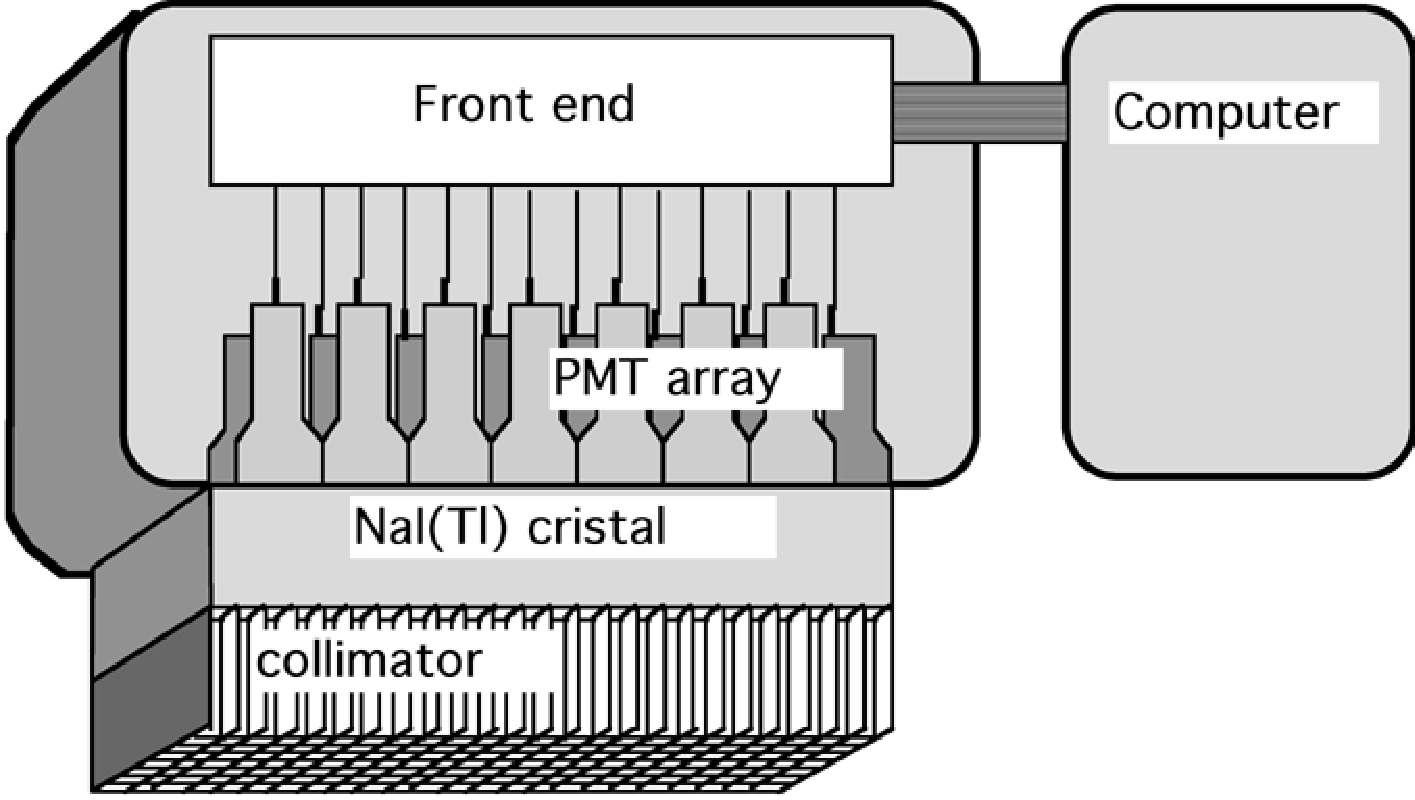
\includegraphics[width=0.5\textwidth]{figs/fig_jngamma.pdf}
\caption{\label{fig:gammacamera} \emph{Schematic representation of a gamma
camera with a single large scintillation crystal and parallel hole
collimator.}}
\end{figure}

\subsection{Linearity correction}
%=================================
\begin{figure}[tb]
\centering
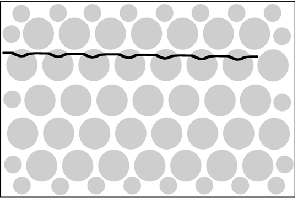
\includegraphics[width=0.5\textwidth]{figs/fig_linearity.pdf}
\caption{\label{fig:linearity} \emph{The PMTs (represented as circles) have a
non-linear response as a function of position. As a result, the image of a
straight radioactive line would be distorted as in this drawing.}}
\end{figure}

In section \ref{sec:single_crystal} we have seen that the position of
a scintillation in a large crystal is computed as the first moment in
$x$ and $y$ directions (the ``mass'' center of the PMT response). This
would be exact if the PMT response would vary linearly with
position. In reality, the response is not perfectly linear, and as a
result, the image is distorted. Figure \ref{fig:linearity} illustrates
how the image of a straight radioactive wire can be deformed by this
non-linear response. The response is systematic, so it can be
measured, and the errors $\Delta_x$ and $\Delta_y$ can be stored as a
function of $x$ and $y$ in a lookup table. Correction is then
straightforward:
\begin{eqnarray}
 x_{\mbox{corrected}} & = & x + \Delta_x(x,y) \nonumber\\
 y_{\mbox{corrected}} & = & y + \Delta_y(x,y)
\end{eqnarray}
After correction, the image of a straight line will be a straight line.

For a system using multi-crystal detectors, the linearity correction must be
applied within the modules, to make sure the correct individual detector is
identified. Because we know exactly where each module and each detector is
located, no further spatial corrections are required.

Because the system characteristics vary slowly in time, the linearity
correction table needs to be measured every now and then. This is typically
once a year or after a major intervention (e.g. after PMTs have been
replaced).

To measure the linearity, we must make an image of a {\em phantom}, a well
known object. One approach is to use a ``dot-phantom'': the collimator is
replaced with a lead sheet containing a matrix of small holes at regular
positions. Then we put some activity in front of the sheet (e.g. we can use a
point source at a large distance from the sheet), ensuring that all holes
receive approximately the same amount of photons. With this set up, an image
is acquired. Deviations between the image and the known dot pattern allow to
compute $\Delta_x(x,y)$ and $\Delta_y(x,y)$.

\subsection{Energy correction}
%=================================
Recall that the energy of the detected photon was computed as the sum of all
PMT responses (section \ref{sec:single_crystal}). Of course, the sum is
dominated by the few PMTs close to the point of scintillation, the other PMT's
receive very few or even no scintillation photons. Because the
PMT-characteristics show small individual differences, the computed energy is
position dependent. This results in small shifts of the computed energy
spectrum with position. The deviations are systematic (they vary only very
slowly in time), so they can be measured and stored, so that a position
dependent correction can be applied:
\begin{equation}
  E_{\mbox{corrected}}(x,y) = E(x,y) + \Delta_E(x,y)
\end{equation}

It is important that the energy window is nicely symmetrical around the
photopeak, small shifts of the window result in significant changes in the
number of accepted photons (figure \ref{fig:energy_corr}). Consequently, if no
energy correction is applied, the sensitivity for acceptable photons would be
position dependent.

\begin{figure}[tb]
\centering
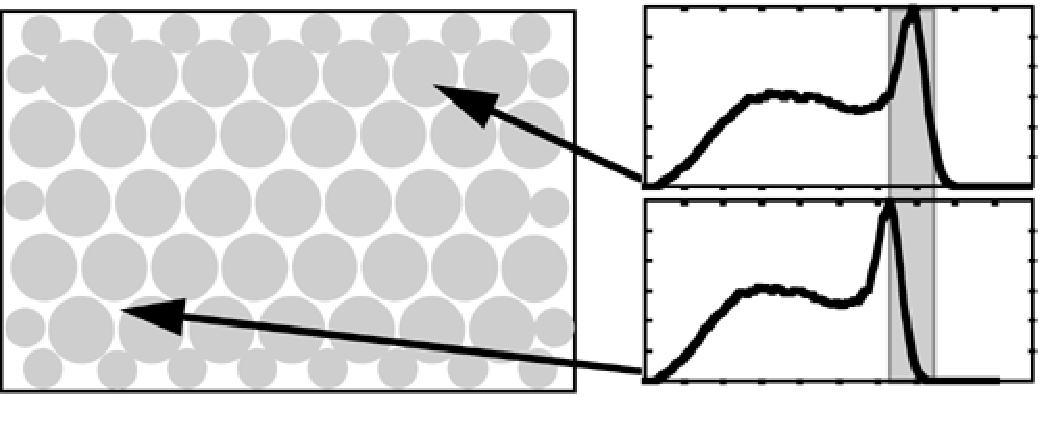
\includegraphics[width=0.5\textwidth]{figs/fig_energy_corr.pdf}
\caption{\label{fig:energy_corr} \emph{Because the characteristics of the
photomultipliers are not identical, the conversion of energy to voltage (and
therefore to a number in the computer) may be position dependent.}}
\end{figure}

The energy correction table needs to be rebuilt about every six months or
after a major intervention. The situation is similar for single crystal and
multicrystal systems.

%%%% TOT HIER NAGEZIEN.

\subsection{Uniformity correction}
%=================================
When linearity and energy correction have been applied, the image of a uniform
activity distribution should be a uniform image. In practice, there may still
be small differences, due to small variations of the characteristics with
position (e.g. crystal transparency, optical coupling between crystal and PMT
etc). Most likely, those are simply differences in sensitivity, so they do not
produce deformation errors, only multiplicative errors. Again, these
sensitivity changes can be measured and stored in order to correct them.

\subsubsection{Gamma camera}
%---------------------------
To measure the uniformity of the detector, we acquire an image of
a uniform activity. For the gamma camera, one approach is to put a
large homogeneous activity in front of the collimator. Another
possibility is to remove the collimator and put a point source at a
large distance in front of the collimator. Let us assume that the
point source is exactly in front of the center of the detector, at a
distance $H$ from the crystal. The number of photons arriving in
position $(x,y)$ per second and per solid angle is then
\begin{equation}
  \mbox{counts  per s and per solid angle} 
     = \frac{A}{4 \pi (H^2 + (x-x_0)^2 +(y-y_0)^2)}
\end{equation}
where $A$ is the strength of the source in Bq (Becquerel), and $(x_0, y_0)$ is
the center of the crystal. However, we don't need the number of
photons per solid angle, but the number of photons per detector
area. At position $(x,y)$, the photons arrive at an angle 
$\alpha = \arctan(\sqrt{(x-x_0)^2 +(y-y_0)^2}/ H)$. Thus, the solid
angle occupied by a small square of detector $dx\ dy$ equals $dx\ dy
\cos(\alpha)$. Because $\cos(\alpha) = H / \sqrt{H^2 + (x-x_0)^2
  +(y-y_0)^2}$, we obtain for the number of photons detected in $dx\
dy$:
\begin{equation}
  \mbox{counts detected in dx dy} 
     = \frac{A H}{4 \pi (H^2 + (x-x_0)^2 +(y-y_0)^2)^{3/2}}
     = \frac{A \cos^3\alpha}{H^2}
\end{equation}
%
Thus, if we know the size of the detector and the uniformity error we
will tolerate we can compute the required distance $H$.  You can
verify that with $H = 5 D$, where $D$ is the length of the crystal diagonal,
the maximum error equals about 1.5\%.

The number of photons detected in every pixel is Poisson distributed. Recall
from section \ref{sec:statistics} that the standard deviation of a Poisson
number is proportional to the square root of the expected value. So if we
accept an error (a standard deviation) of 0.5\%, we need to continue the
measurement until we have about 40000 counts per pixel. Computation of the
uniformity correction matrix is straightforward:
\begin{equation}
  \mbox{sensitivity\_corr}(x,y) = \frac{\mbox{mean}(I)}{I(x,y)}
\end{equation}
where $I$ is the acquired image.

Consequently, if a uniformity correction is applied to a planar image, one
Poisson variable is divided by another one. The relative noise variance in
the corrected image will be the sum of the relative noise variances on the
two Poisson variables (see appendix \ref{app:error} for estimating the error
on a function of noisy variables).

\subsubsection{PET camera} \label{sec:normalization1}
%-------------------------
In PET-vocabulary, uniformity correction is often called {\em detector
normalization}. The approach is similar as for the gamma camera, but
it is more difficult to measure the relative sensitivity of each
projection line than it is for a gamma camera.  One approach is to
slowly rotate a flat homogeneous phantom in the field of view, and
only use measurements along projection lines (nearly) perpendicular to
the phantom. It is time consuming, since most of the acquired data is
ignored, but it provides a direct sensitivity measurement for all
projection lines.

Alternatively, an indirect approach can be used. A sinogram is acquired for a
large phantom in the center of the field of view. All individual detectors
contribute to the measurement, and each detector is involved in multiple
projection lines intersecting the phantom. However, many other detector pairs
are not receiving photons at all. This measurement is sufficient to compute
individual detector sensitivities. Sensitivity of a projection line can then
be computed from the individual detector sensitivity and the known geometry.
The result is a sinogram representing projection line sensitivities. This
sinogram can be used to compute a correction for every sinogram pixel:
\begin{equation}
  \mbox{normalization}(i) = 
    \frac{\mbox{mean(sensitivity)}}{\mbox{sensitivity}(i)}. \label{eq:petnorm}
\end{equation}
A typical sensitivity sinogram is shown in figure
\ref{fig:pet_norm}. The sinogram is dominated by a regular pattern of
zero sensitivity projection lines, which are due to small gaps between
the detector blocks. In the projections one can see that there is a
significant axial variation in the sensitivities. After normalization,
the data from a uniform cylinder are indeed fairly uniform, except for
these zero sensitivities. In iterative reconstruction, the data in
these gaps are simply not used. For filtered backprojection, these
data must first be filled with some interpolation algorithm.
%
\begin{figure}[tb]
\centering
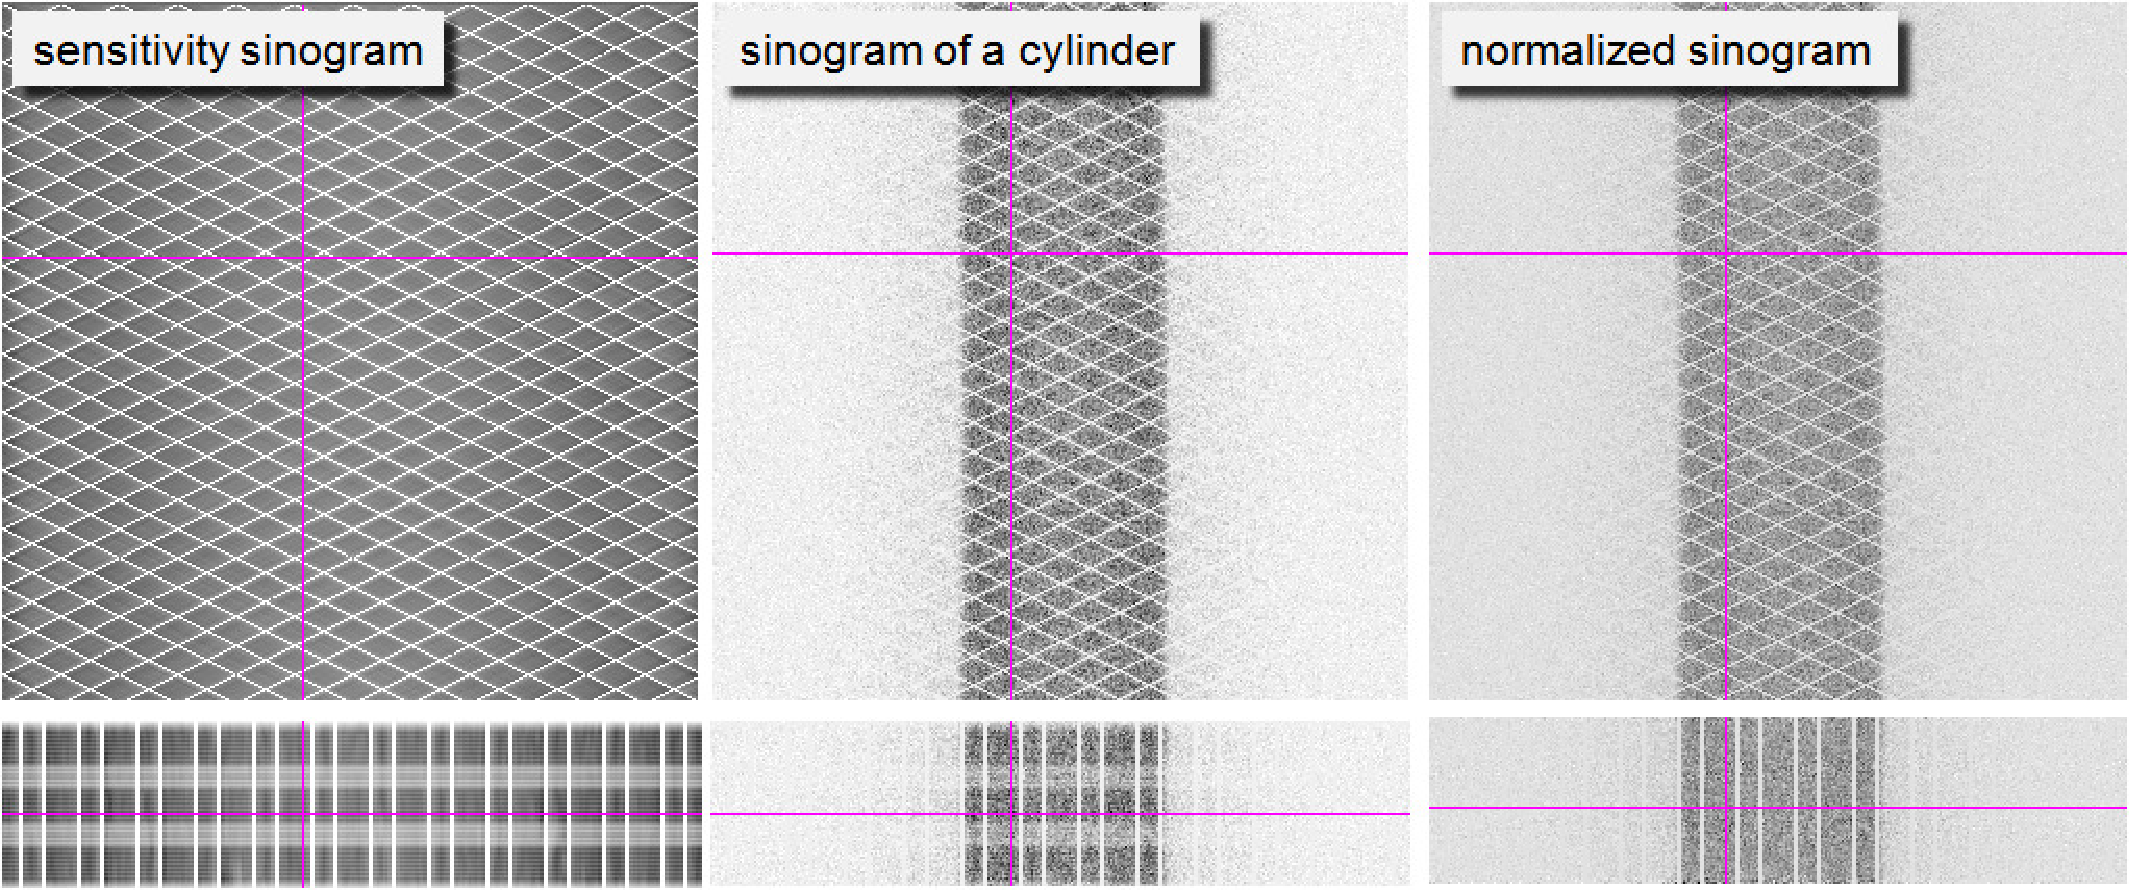
\includegraphics[width=0.9\textwidth]{figs/fig_PETsens.pdf}
\caption{\label{fig:pet_norm} \emph{Left: PET sensitivity
    sinogram. Center: the sinogram of a cylinder filled with a uniform
    activity. Right: the same sinogram after normalization. The first
    row are sinograms, the second row projections, the cross-hairs
    indicate the relative position of both. Because there are small
    gaps between detector blocks, there is a regular pattern of zero
    sensitivity projection lines, which are of course not corrected by the
    normalization.}}
\end{figure}


\subsection{Dead time correction} \label{sec:deadtime}
%=================================
``Dead time'' means that the system has a limited data processing capacity. If
the data input is too high, a fraction of the data will be ignored because of
lack of time. As a result, the measured count rate is lower than the true
count rate, and the error increases with increasing true count rate. Figure
\ref{fig:dead_time} shows the measured count rate as a function of the true
count rate for a dead time of 700 ns. The gamma camera and the PET camera both
have a finite dead time, consisting of several components. To describe the
dead time, we will assume that all contributions can be grouped in two
components, a front-end component and a data-processing component.

\begin{figure}[tb]
\centering
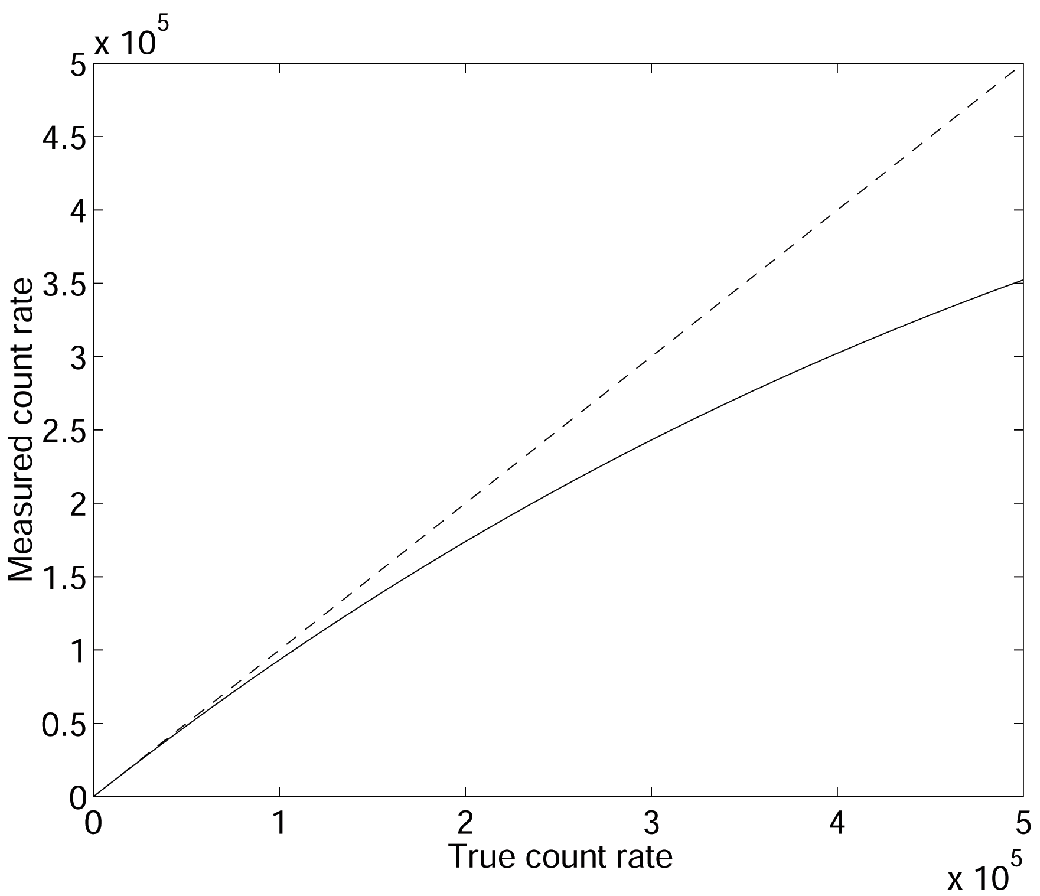
\includegraphics[width=0.5\textwidth]{figs/fig_dead_time.pdf}
\caption{\label{fig:dead_time} \emph{Due to dead time, the measured count rate
is lower than the true count rate for high count rates. The figure is for a
dead time of 700 ns, the axes are in counts per second. Measured count rate is
20\% low near 300000 counts per second.}}
\end{figure}

\subsubsection{Front-end dead time}
%------------------------------------
Recall (section \ref{sec:single_crystal}) that the scintillation has
a finite duration. E.g., the decay time of NaI(Tl) is 230 ns. The PMT
response time adds a few ns. To have an accurate estimate of the
energy, we need to integrate over a sufficient fraction of the
PMT-outputs, such that most of the scintillation photons get the
chance to contribute. Let us assume that the effective scintillation
time is $\tau_1 / 2$, and that we integrate over that time to compute
position and energy. Then the result is only correct if no new
scintillation starts during that period, and no old one is ending
during that period (so the previous scintillation must be older than
$\tau_1/2$).  Otherwise, part of this other scintillation will
contribute as well, the energy will be overestimated and the photon is
rejected. Consequently, a photon is only detected if in a time
$\tau_1$ exactly one photon arrives.  If we have a true count rate of
$R_0$, then we expect $R_0 \tau_1$ photons in the interval
$\tau_1$. Recall that the number of photons is Poisson distributed, so
the probability of having 1 photon when $R_0 \tau_1$ are expected is
$\exp(- R_0 \tau_1) R_0 \tau_1$. This is the count per time $\tau_1$,
so the count rate of accepted events will be
\begin{equation}
  R_1 = R_0 e^{-R_0 \tau_1}. \label{eq:deadtime_front}
\end{equation}
Notice that if $R_0$ is extremely large, $R_1$ goes to zero: the system is
said to be {\em paralyzable}. Indeed, if the count rate is extremely high,
every scintillation will be disturbed by the next one, and the camera will
accept no events at all.

\subsubsection{Data-processing dead time}
%------------------------------------
When the event is accepted, the linearity correction must be applied and it
must be stored somehow: the electronics either stores it in a list, and
increments the pointer to the next available address, or it increments the
appropriate location in the image. This takes time, let us say $\tau_2$. If
during that time another event occurs, it is simply ignored. Consequently, a
fraction of the incoming events will be missed, because the electronics is not
permanently available.

Assume that the electronics needs to store data at a rate of $R_2$ (unit
$s^{-1}$). Each of these requires $\tau_2$ s, so in every second, $R_2 \tau_2$
are already occupied for processing data. The efficiency of the system is
therefore $1 - \tau_2 R_2$, which gives us the relation between incoming count
rate $R_1$ and processed count rate $R_2$:
\begin{equation}
  R_2 = (1 - R_2 \tau_2) R_1
\end{equation}
Rearranging this to obtain $R_2$ as a function of $R_1$ results in
\begin{equation}
  R_2 = \frac{R_1}{1 + R_1 \tau_2}. \label{eq:deadtime_proc}
\end{equation}
This function is monotonically increasing with upper limit $1 /
\tau_2$ (as you would expect: this is the number of intervals of
length $\tau_2$ in one second).  Consequently, the electronics is
non-paralyzable. You cannot paralyze it, but you can saturate it: if
you put in too much data, it simply performs at maximum speed ignoring
all the rest.

\subsubsection{Effective dead time}
%------------------------------------
Combining (\ref{eq:deadtime_front}) and (\ref{eq:deadtime_proc}) tells us the
acceptance rate for an incident photon rate of $R_0$:
\begin{equation}
  R_2 = \frac{R_0 e^{-R_0 \tau_1}}{ 1 + R_0 e^{-R_0 \tau_1} \tau_2}.
\end{equation}
If the count rates are small compared to the dead times (such that $R_x
\tau_y$ is small), we can introduce an approximation to make the
expression simpler. The approximation is based on the following relations,
which are acceptable if $x$ is small:
\begin{eqnarray}
  e^{-x} & \simeq & e^{-0} + x \left. \frac{d e^{-x}}{dx} \right|_{x=0}= 1-x\\
         & = & \frac{1+x}{1+x} - x = \frac{1+x-x-x^2}{1+x} 
        \simeq \frac{1}{1 + x}.
\end{eqnarray}
Applying this to (\ref{eq:deadtime_front}) and (\ref{eq:deadtime_proc}) yields:
\begin{eqnarray}
  R_1 & \simeq & R_0 (1 - R_0 \tau_1)\\
  R_2 & \simeq & R_1 (1 - R_1 \tau_2)
\end{eqnarray}
Combining both equation and deleting higher order terms results in
\begin{eqnarray}
  R_2 & \simeq & R_0 \left(1 - R_0 (\tau_1 + \tau_2) \right) \label{eq:dead1}\\
      & \simeq & R_0 e^{- R_0 (\tau_1 + \tau_2)} \label{eq:dead2}
\end{eqnarray}
So if the count rate is relatively low, there is little difference between
paralyzable and non-paralyzable dead time, and we can obtain a global dead
time for the whole machine by simply adding the contributing dead times.  Most
clinical gamma cameras and all PET systems provide dead time correction based
on some dead time model. However, for very high count rates the models are no
longer valid and the correction will not be accurate.

\subsection{Random coincidence correction} \label{sec:randoms}
%=========================================
The random coincidence was defined in section \ref{sec:petcollim}: two
non-related events may be detected simultaneously and be interpreted as a
coincidence. There is no way to discriminate between true and random
coincidences. However, there is a ``simple'' way to measure a reliable
estimate of the number of randoms along every projection line. This is done
via the delayed window technique.

The number of randoms (equation (\ref{eq:pet_randoms})) was obtained by
squaring the probability to measure a single event during a time window
$\tau$. In the delayed window technique, an additional time window is used,
which is identical in length to the normal one but delayed over a short time
interval. The data for the second window are monitored with the same
coincidence electronics and algorithms as used for the regular coincidence
detection, ignoring the delay between the windows. If a coincidence is
obtained between an event in the normal and an event in the delayed window,
then we know it has to be a random coincidence: because of the delay the
events cannot be due to the same annihilation. Consequently, with regular
windowing we obtain {\em trues + randoms1}, and with the delayed method we
obtain a value {\em randoms2}. The values {\em randoms1} and {\em randoms2}
are not identical because of Poisson noise, but at least their expectations
are identical. Subtraction will eliminate the bias, but will increase the
variance on the estimated number of trues. See appendix \ref{app:error} for
some comments on error propagation.

\chapter{Image formation}  \label{ch:image_formation}

% Wat meten we: CT, PET, SPECT (attenuated projection)
%--------------
% planar
%--------
%
% 2D Tomography
%-----------
%
% Fully 3D Tomography
%-----------
%
% Mathematical model of the acquisition process
%-----------
\begin{figure}[tb]
\centering
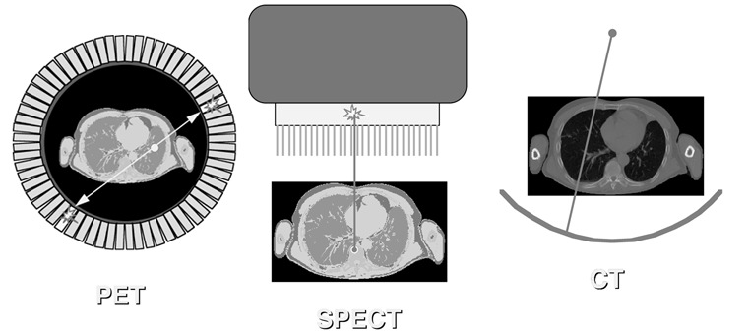
\includegraphics[width=0.75\textwidth]{figs/fig_spect_pet_ct.pdf}
\caption{\label{fig:spect_pet_ct_bis} \emph{Information acquired along lines
in the PET camera, the gamma camera and the CT-scanner.}}
\end{figure}

\section{Introduction}
%%%%%%%%%%%%%%%%%%%%%%
The tomographic systems are shown (once again) in figure
\ref{fig:spect_pet_ct_bis}. They have in common that they perform an indirect
measurement of what we want to know: we want to obtain information about the
distribution in every point, but we acquire information integrated over
projection lines. So the desired information must be computed from the
measured data. In order to do that, we need a mathematical function that
describes (simulates) what happens during the acquisition: this function is an
operator that computes measurements from distributions. If we have that
function, we must derive its inverse: this will be an operator that computes
distributions from measurements.

In the previous chapters we have studied the physics of the acquisition, so we
are ready to compose the acquisition model. We can decide to introduce some
approximation to obtain a simple acquisition model, hoping that deriving the
inverse will not be too difficult. The disadvantage is that the inverse
operator will not be an accurate inverse of the true acquisition process, so
the computed distribution will not be identical to the true distribution. On
the other hand, if we start from a very detailed acquisition model, inverting
it may become mathematically and/or numerically intractable.

For a start, we will assume that collimation is perfect and that there is no
noise and no scatter. We will only consider the presence of radioactivity
and attenuating tissue.

Consider a single projection line in the CT-camera. We define the $s$-axis
such that it coincides with the line. The source is at $s=a$, the detector at
$s = b$. A known amount of photons $t_0$ is emitted in $a$ towards the
detector element at $b$. Only $t(b)$ photons arrive, the others have been
eliminated by attenuation. If $\mu(s)$ is the linear attenuation coefficient
in the body of the patient at position $s$, we have (see also eq
(\ref{jn:spectatten}))
\begin{equation}
  t(b) = t_0 e^{- \int_a^b \mu(s) ds}. \label{eq:ct_proj}
\end{equation}
The exponential gives the probability that a photon emitted in $a$ towards $b$
is not attenuated and arrives safely in $b$.

For a gamma camera measurement, there is no transmission source. Instead, the
radioactivity is distributed in the body of the patient. We must integrate the
activity along the $s$-axis, and attenuate every point with its own
attenuation coefficient. Assuming again that the patient is somewhere between
the points $a$ and $b$ on the $s$-axis, then the number of photons $q$ arriving
in $b$ is:
\begin{equation}
  q(b) = \int_a^b \lambda(s) e^{- \int_s^b \mu(\xi) d\xi} ds,
   \label{eq:spect_proj}
\end{equation}
where $\lambda(s)$ is the activity in $s$.
For the PET camera, the situation is similar, except that it must detect both
photons. Both have a different probability of surviving attenuation. Since the
detection is only valid if both arrive, and since their fate is independent,
we must multiply the survival probabilities:
\begin{eqnarray}
  q(b) & = & \int_a^b \lambda(s) e^{- \int_a^s \mu(\xi) d\xi} 
                             e^{- \int_s^b \mu(\xi) d\xi} ds \\
  & = & e^{- \int_a^b \mu(\xi) d\xi} \int_a^b \lambda(s) ds.
        \label{eq:pet_proj}
\end{eqnarray}

In CT, only the attenuation coefficients are unknown. In emission tomography,
both the attenuation and the source distribution are unknown. In PET, the
attenuation is the same for the entire projection line, while in single photon
emission, it is different for every point on the line.

It can be shown (and we will do so below) that it is possible to reconstruct
the planar distribution, if all line integrals (or projections) through a
planar distribution are available. As you see from figure
\ref{fig:spect_pet_ct_bis}, the gamma camera and the CT camera have to be
rotated if all possible projections must be acquired. In contrast, a PET ring
detector acquires all projections simultaneously (with ``all'' we mean here a
sufficiently dense sampling).

\section{Planar imaging}
%%%%%%%%%%%%%%%%%%%%%%%%
% Scatter
% Count rate, dead time
Before discussing how the activity and/or attenuation distributions can be
reconstructed, it is interesting to have a look at the raw data. For a gamma
camera equipped with parallel hole collimator, the raw data are naturally
organized as interpretable images, ``side views'' of the tracer concentration
in the transparent body of the patient. For a PET camera, the raw data can be
organized in sets of parallel projections as well, as shown in figure
\ref{fig:pet_parallel}. 

\begin{figure}[tb]
\centering
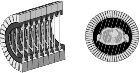
\includegraphics[width=0.5\textwidth]{figs/fig_pet_parallel.pdf}
\caption{\label{fig:pet_parallel} \emph{Raw PET data can be organized in
parallel projections, similar as in the gamma camera.}}
\end{figure}

\begin{figure}[tb]
\centering
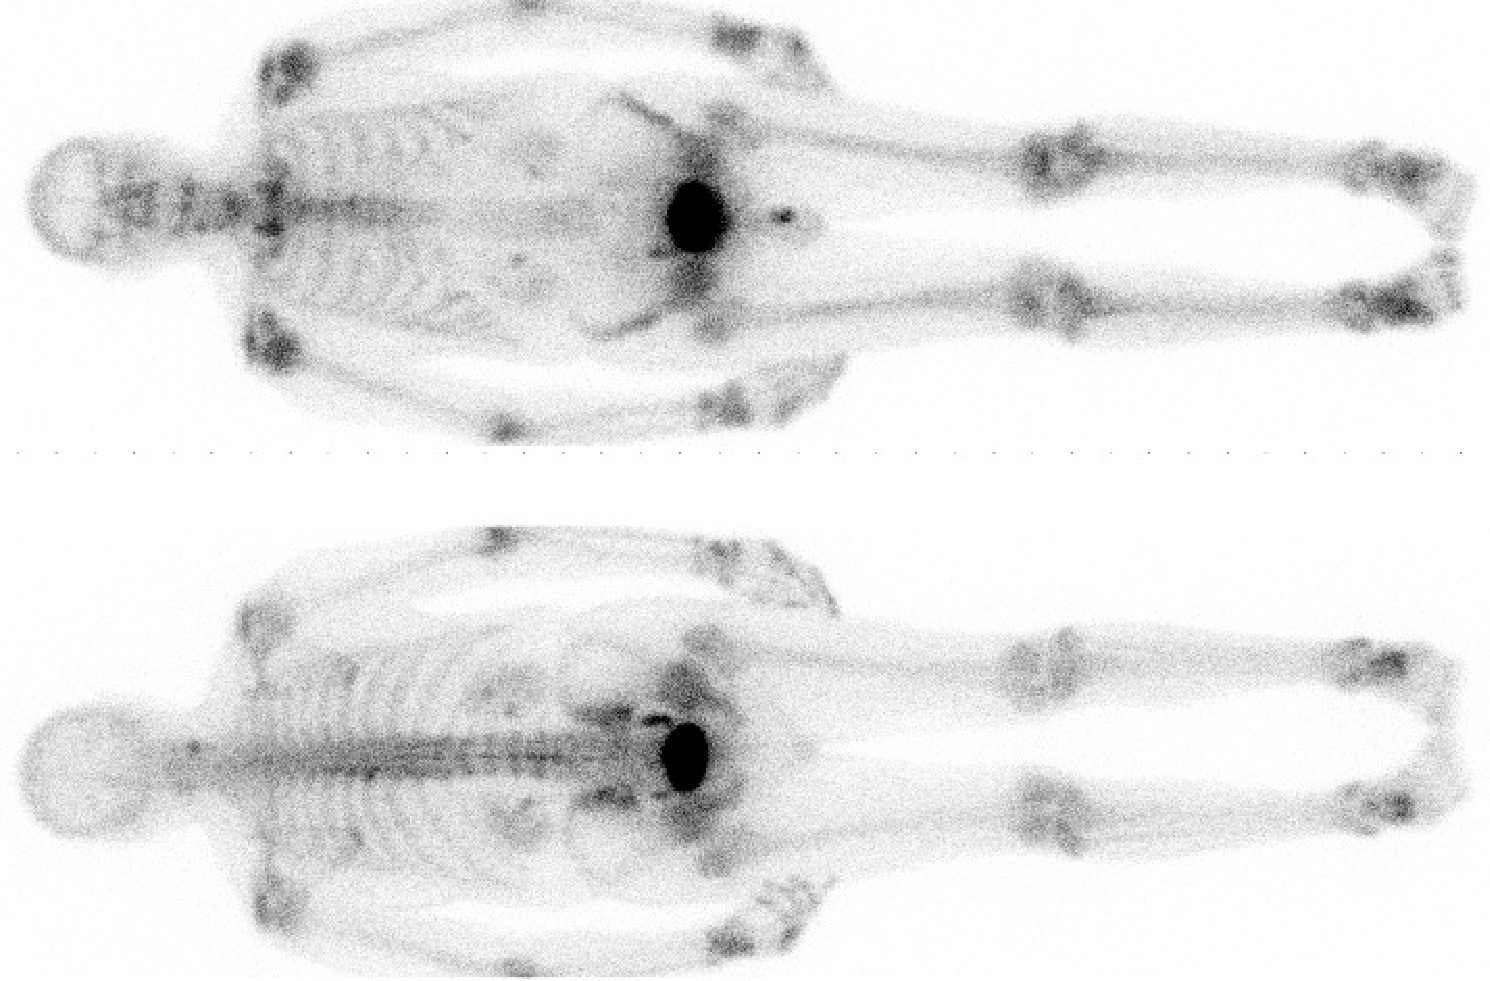
\includegraphics[width=0.5\textwidth]{figs/fig_jnwb.pdf}
\caption{\label{fig:planarwb} \emph{\textsuperscript{99m}Tc-MDP study acquired on a dual
head gamma camera. Detector size is about 40 $\times$ 50 cm, the whole body
images are acquired with slow translation of the patient bed. MDP accumulates
in bone, allowing visualization of increased bone metabolism. Due to
attenuation, the spine is better visualized on the posterior image.}}
\end{figure}

Figure \ref{fig:planarwb} shows a planar whole body image, which is obtained
by slowly moving the gamma camera over the patient and combining the
projections into a single image. In this case, a gamma camera with two opposed
detector heads was used, so the posterior and anterior views are acquired
simultaneously. There is no rotation, these are simply raw data, but they
provide valuable diagnostic information. A similar approach is applied in
radiological studies: with the CT tomographic images can be produced, but the
planar images (e.g. thorax X-ray) already provide useful information. 

\begin{figure}[tb]
\centering
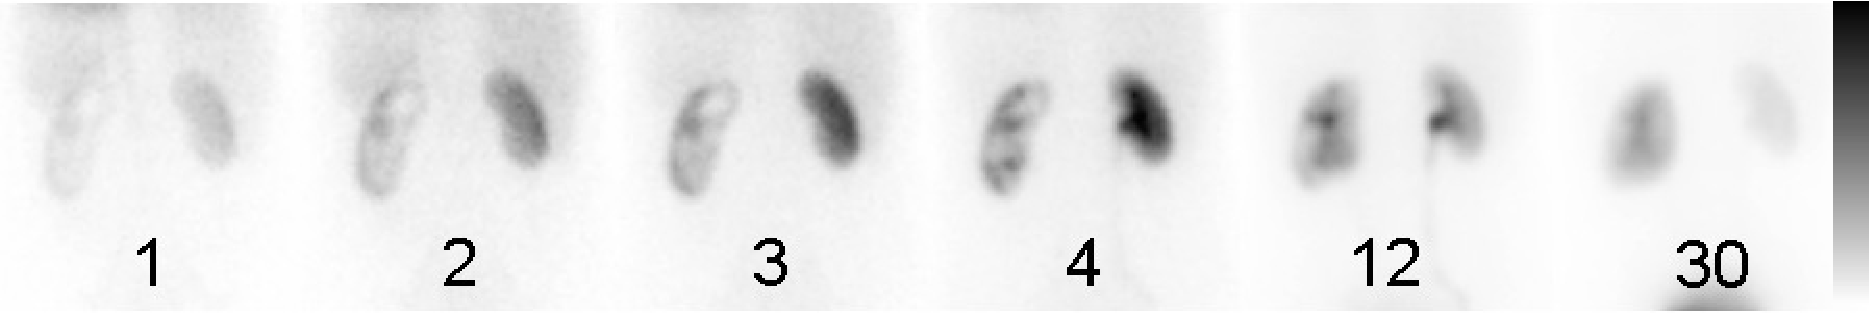
\includegraphics[width=0.9\textwidth]{figs/fig_renaldynimg.pdf}
\caption{\label{fig:renaldyn} \emph{A few images from a
    renography. The numbers are the minutes after injection of the
    \textsuperscript{99m}Tc-labeled tracer. The left kidney (at the right in the
    image) is functioning normally, the other one is not: both uptake
    and clearance of the tracer are slowed down.}}
\end{figure}

\begin{figure}[tb]
\centering
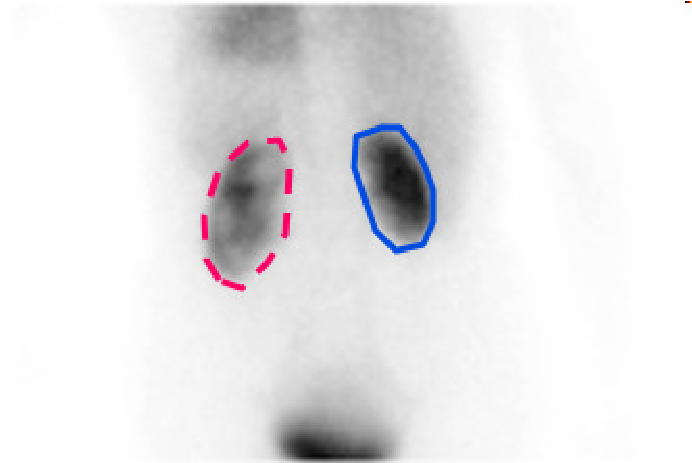
\includegraphics[width=0.45\textwidth]{figs/fig_renalrois.pdf}
  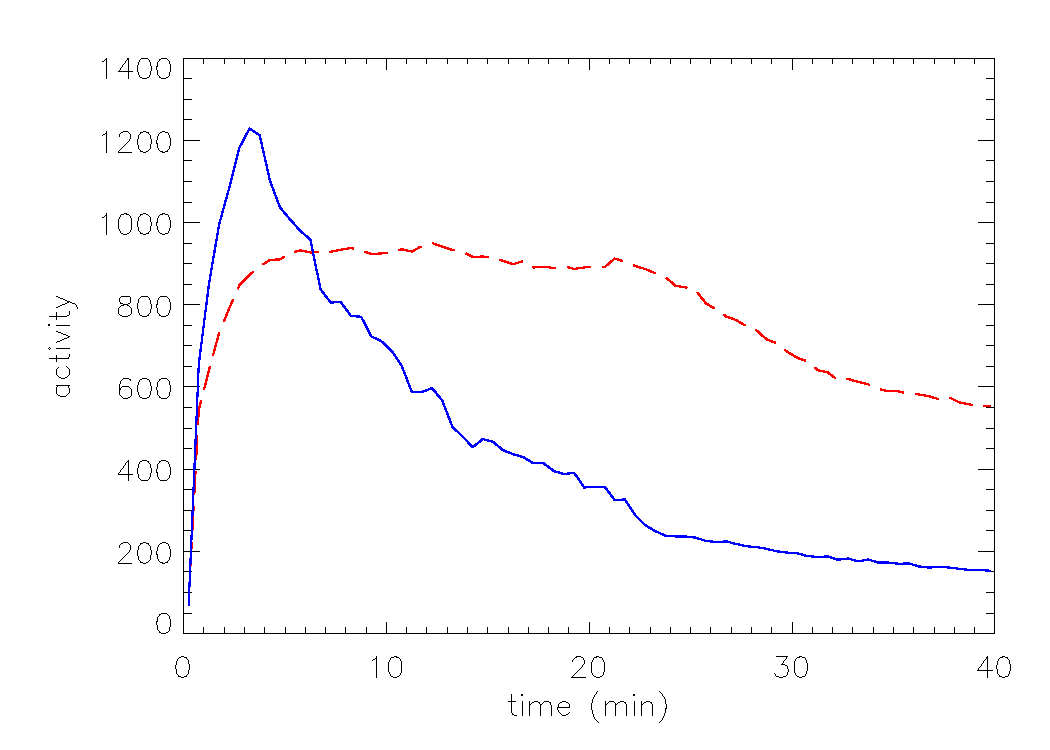
\includegraphics[width=0.5\textwidth]{figs/fig_renalplot.pdf}
\caption{\label{fig:renalroi} \emph{Summing all frames of the dynamic
    renal study yields the image on the left, where the kidneys can be
    easily delineated. The total count in these regions as a function
    of time (time activity curves or TACs) are shown on the right,
    revealing a distinct difference in kidney function.}}
\end{figure}

The dynamic behaviour of the tracer can be measured by acquiring a
series of consecutive images. To study the function of the kidneys, a
\textsuperscript{99m}Tc\ labeled tracer (in this example ethylene dicysteine, known
as \textsuperscript{99m}Tc-EC) is injected, and its renal uptake is studied over
time. The first two minutes after injection, 120 images of 1 s are
acquired to study the perfusion. Then, about a hundred planar images
are acquired over 40 min to study the clearance. Fig
\ref{fig:renaldyn} and \ref{fig:renalroi} show the results in a
patient with one healthy and one poorly functioning kidney.

The study duration should not be too long because of patient
comfort. A scanning time of 15 min or half an hour is reasonable, more
is only acceptable if unavoidable. If that time is used to acquire a
single or a few planar images, there will be many photons per pixel
resulting in good signal to noise ratio, but there is no depth
information.  If the same time is used to acquire many projections for
tomographic reconstruction, then there will be few counts per pixel
and more noise, but we can reconstruct a three-dimensional image of
the tracer concentration. The choice depends on the application.

In contrast, planar PET studies are very uncommon, because most PET-cameras
are acquiring all projections simultaneously, so the three-dimensional image
can always be reconstructed.

\section{2D Emission Tomography}
%%%%%%%%%%%%%%%%%%%%%%%
% Sinogram
% FBP
% MLEM
% Randoms correction
% Scatter correction
% Collimator blurring

In this section, we will study the reconstruction of a planar distribution
from its line integrals. The data are two-dimensional: a projection line is
completely specified by its angle and its distance to the center of the field
of view. A two-dimensional image that uses $d$ as the column coordinate and
$\theta$ as the row coordinate is called a {\em sinogram}. Figure
\ref{fig:sinogram} shows that the name is well chosen: the sinogram of point
source is zero everywhere except on a sinusoidal curve. The sinogram in the
figure is for 180\textdegree. A sinogram for 360\textdegree\ shows a full period of
the sinusoidal curve. It is easy to show that, using the conventions of figure
\ref{fig:sinogram}, $s(x,y) = s_x + s_y = x \cos \theta + y \sin \theta$, so
the non-zero projections in the sinogram are indeed following a sinusoidal
curve.

\begin{figure}[tb]
\centering
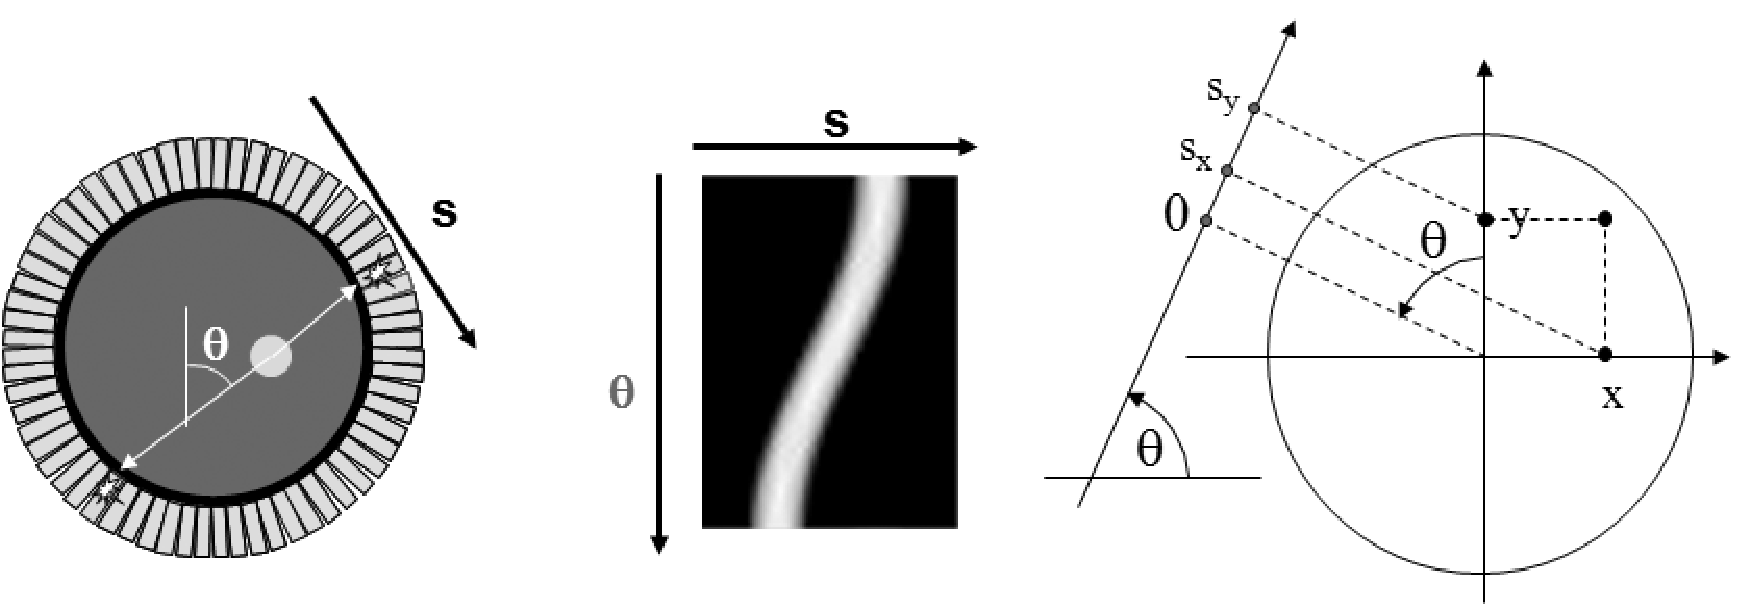
\includegraphics[width=0.9\textwidth]{figs/fig_sinogram.pdf}
\caption{\label{fig:sinogram} \emph{A sinogram is obtained by storing the 1D
parallel projections as the rows in a matrix (or image). Left: the camera with
a radioactive disk. Center: the corresponding sinogram. Right: the
conventions, $\theta$ is positive in clockwise direction.}}
\end{figure}

\subsection{2D filtered backprojection}
%=================================
Filtered backprojection (FBP) is the mathematical inverse of an idealized
acquisition model: it computes a two-dimensional continuous distribution from
ideal projections. In this case, ``ideal'' means the following:
\begin{itemize}
\item
The distribution has a finite support: it is zero, except within a finite
region.  We assume this region is circular (we can always do that, since the
distribution must not be non-zero within the support). We assume that this
region coincides with the field of view of the camera. We select the center of
the field of view as the origin of a two-dimensional coordinate system.

\item
Projections are continuous: the projection is known for every angle and for
every distance from the origin. Projections are ideal: they are unweighted
line integrals (so there is no attenuation and no scatter, the PSF is a Dirac
impulse and there is no noise).

\item
The distribution is finite everywhere. That should not be a problem in real
life.

\end{itemize}

\subsubsection{Projection}
%------------------------------------
\begin{figure}[tb]
\centering
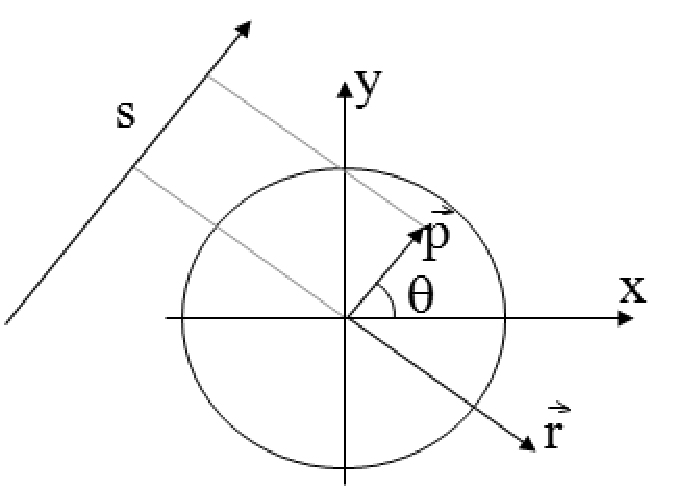
\includegraphics[width=0.35\textwidth]{figs/fig_fbp_math.pdf}
\caption{\label{fig:fbp_math} \emph{The projection line as a function of a
single parameter $r$. The line consists of the points $\vec{p} + \vec{r}$,
with $\vec{p} = (s \cos \theta, s \sin \theta)$, $\vec{r} = (r \sin \theta, - r
\cos \theta)$.}}
\end{figure}

Such an ideal projection $q$ is then defined as follows (using the conventions
of figure \ref{fig:sinogram}):
\begin{eqnarray}
q(s, \theta) & = &\int_{(x,y) \in \; \mbox{projection line}}
                  \lambda(x,y) dx dy\\
             & = &\int_{-\infty}^{\infty}
        \lambda(s \cos \theta + r \sin \theta,
                s \sin \theta - r \cos \theta) dr. \label{eq:jnidealproj}
\end{eqnarray}
The point $(s \cos \theta, s \sin \theta)$ is the point on the projection line
closest to the center of the field of view.  By adding $(r \sin \theta, - r
\cos \theta)$ we take a step $r$ along the projection line (fig
\ref{fig:fbp_math}).


\subsubsection{The Fourier theorem}
%------------------------------------
The Fourier theorem (also called the {\em central slice theorem})
states that there is a simple relation between the one-dimensional
Fourier transform of the projection $q(s, \theta)$ and the
two-dimensional Fourier transform of the distribution $\lambda(x,y)$.

The Fourier theorem is very easy to prove for projection along the y-axis (so
$\theta = 0$). Because the y-axis may be chosen arbitrarily, it holds for
any other projection angle (but the notation gets more elaborate).
In the following $Q$ is the 1-D Fourier transform (in the first coordinate) of
$q$. Because the angle is fixed and zero, we have
$q(s, \theta) = q(s, 0) = q(x,0)$.
\begin{eqnarray}
  q(x,0) & = & \int_{-\infty}^{\infty} \lambda(x,y) dy \\
  Q(\nu_x,0) & = & \int_{-\infty}^{\infty}  q(x,0) e^{-j2\pi \nu_x x} dx \\
          & = & \int_{-\infty}^{\infty}  \int_{-\infty}^{\infty}
                 \lambda(x,y) e^{-j2\pi \nu_x x} dx dy.
\end{eqnarray}
Here, $j = \sqrt{-1}$. Let us now compute the 2-D Fourier transform
$\Lambda$ of $\lambda$:
\begin{equation}
\Lambda(\nu_x, \nu_y)  =   \int_{-\infty}^{\infty}  \int_{-\infty}^{\infty}
         \lambda(x,y) e^{-j2\pi (\nu_x x + \nu_y y)} dx dy.
\end{equation}
So it immediately follows that $\Lambda(\nu_x, 0) = Q(\nu_x)$.
Formulated for any angle $\theta$ this becomes:
\begin{equation}
  \Lambda(\nu \cos \theta, \nu \sin \theta) = Q(\nu, \theta). 
  \label{fouriertheorem}
\end{equation}
A more rigorous proof for any angle $\theta$ is given in appendix
\ref{app:cs}.  In words: the 1-D Fourier transform of the projection
acquired for angle $\theta$ is identical to a central profile along
the same angle through the 2-D Fourier transform of the original
distribution (fig \ref{fig:fouriertheorem}).

\begin{figure}[tb]
\centering
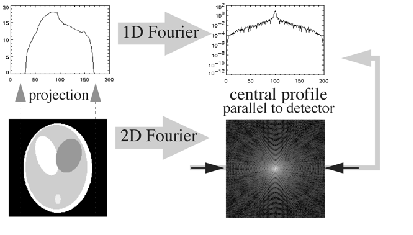
\includegraphics[width=0.6\textwidth]{figs/fig_fouriertheorem.pdf}
\caption{\emph{The Fourier theorem.}}
\label{fig:fouriertheorem} 
\end{figure}

The Fourier theorem directly leads to a reconstruction algorithm by simply
digitizing everything: compute the 1D FFT transform of the projections for
every angle, fill the 2D FFT image by interpolation between the radial 1D FFT
profiles, and compute the inverse 2D FFT to obtain the original distribution.

Obviously, this will only work if we have enough data. Every projection
produces a central line through the origin of the 2D frequency space. We need
to have an estimate of the entire frequency space, so we need central lines
over at least 180 degrees (more is fine but redundant).  Figure
\ref{fig:jnproj_sino} shows clinical raw emission data acquired for
tomography. They can be organized either as projections or as
sinograms. There are typically in the order of 100 (SPECT) or a few hundreds
(PET) of projection angles. The figure shows 9 of them. During a clinical
study, the gamma camera automatically rotates around the patient to acquire
projections over 180\textdegree or 360\textdegree. Because the spatial resolution
deteriorates rapidly with distance to the collimator, the gamma camera not
only rotates, it also moves radially as close as possible to the patient to
optimize the resolution.

As mentioned before, the PET camera consisting of detector rings measures all
projection lines simultaneously, no rotation is required.

\begin{figure}[tb]
\centering
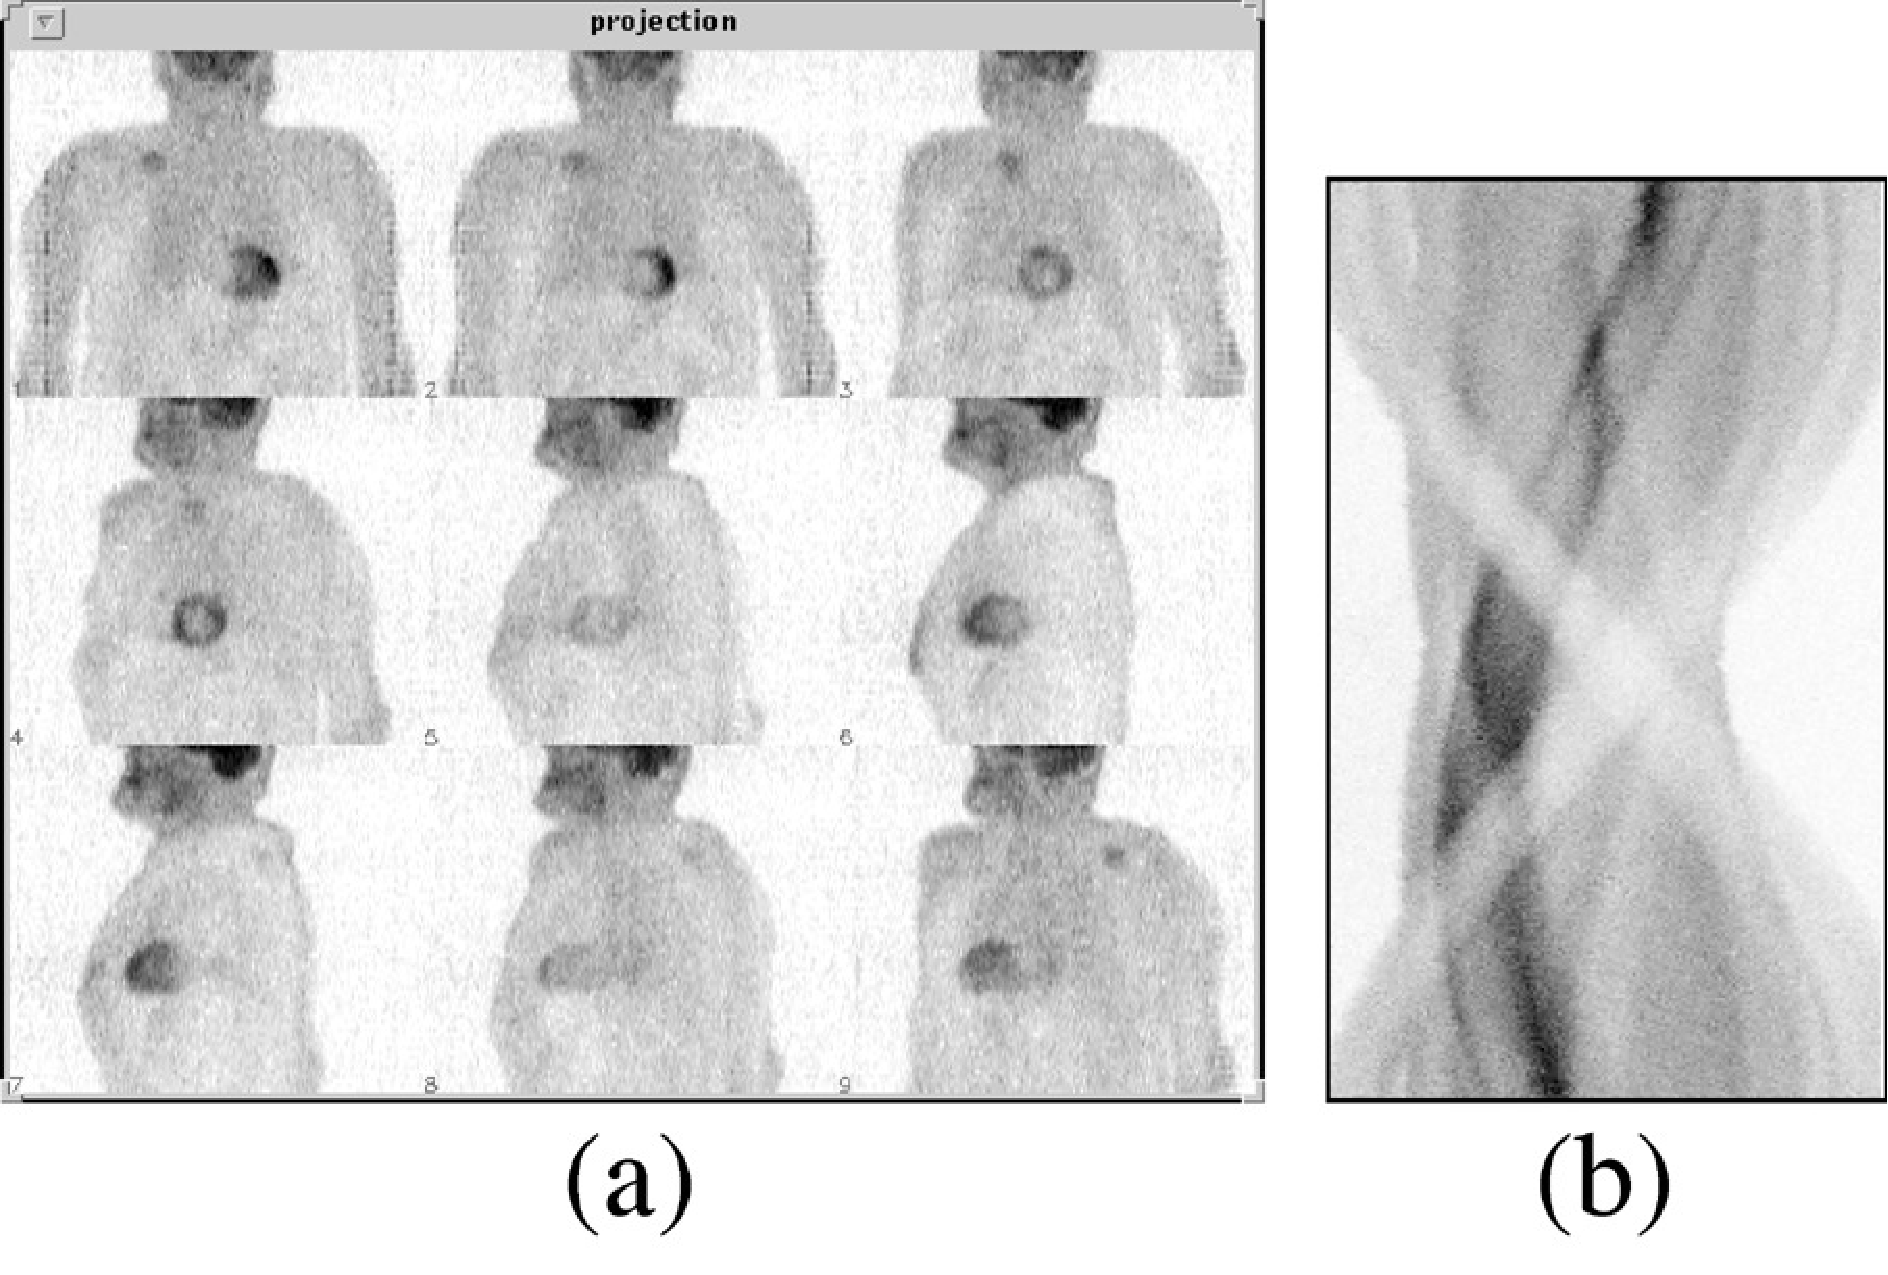
\includegraphics[width=0.72\textwidth]{figs/fig_jnproj_sino.pdf}
\caption{\label{fig:jnproj_sino} \emph{Raw PET data, organized as projections
(a) or as a sinogram (b). There are typically a few hundred projections, one
for each projection angle, and several tens to hundred sinograms, one
for each slice through the patient body}}
\end{figure}


\subsubsection{Backprojection} \label{sec:backprojection}
%------------------------------------
This Fourier-based reconstruction works, but usually an alternative expression
is used, called ``filtered backprojection''. To explain it, we must first define
the operation {\em backprojection}:
\begin{eqnarray}
 b(x,y) & = & \int_0^\pi q(x \cos \theta + y \sin \theta, \theta) d \theta
             \nonumber\\
      & = & \mbox{Backproj} \left( q(s, \theta) \right). \label{eq:jnbackproj}
\end{eqnarray}

\begin{figure}[tb]
\centering
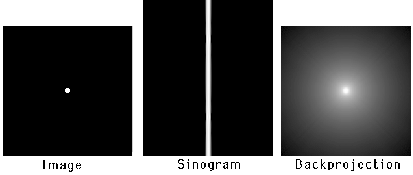
\includegraphics[width=0.6\textwidth]{figs/fig_backproj.pdf}
\caption{\label{fig:backproj} \emph{A point source, its sinogram and the
backprojection of the sinogram (logarithmic gray value scale).}}
\end{figure}

During backprojection, every projection value is uniformly distributed
along its projection line. Since there is exactly one projection line
passing through $(x,y)$ for every angle, the operation involves
integration over all angles. This operation is {\em NOT} the inverse
of the projection. As we will see later on, it is the {\em adjoint
operator} of projection. Figure \ref{fig:backproj} shows the
backprojection image using a logarithmic gray value scale. The
backprojection image has no zero pixel values!

Let us compute the values of the backprojection image from the
projections of a point source. Because the point is in the origin, the
backprojection must be radially symmetrical. The sinogram is zero
everywhere except for $s = 0$ (fig \ref{fig:backproj}), where it is
constant, say $A$. So in the backprojection we only have to consider the
central projection lines, the other lines contribute nothing to the
backprojection image.  Consider the line integral along a circle
around the center (that is, the sum of all values on the circle). The
circle intersects every central projection line twice, so the total
activity the circle receives during backprojection is
\begin{equation}
  \mbox{total circle value} = 2 \int_0^\pi q(0, \theta) d \theta = 2 A\pi.
  \label{eq:bprojvalue}
\end{equation}
So the line integral over a circle around the origin is a constant. The value
in every point of a circle with radius $R$ is $2 A \pi / (2 \pi R) =
A/R$. In conclusion, starting with an image $f(x,y)$ which is zero everywhere,
except in the center where it equals $A$, we find:
\begin{eqnarray}
  f(x,y) & = & A \delta(x) \delta(y)\\
 b(x,y) & = & (\mbox{backproj}(\mbox{proj}(f))(x,y) \; = \;
  \frac{A}{\sqrt{x^2 + y^2}}.
\end{eqnarray}
A more rigorous derivation is given in appendix \ref{app:bprojproj}.

Projection followed by backprojection is a linear operation. In the
idealized case considered here, it is also a shift invariant
operation. Consequently, we have actually computed the point spread function
of that operation.

\subsubsection{Filtered backprojection}
%------------------------------------
Filtered backprojection follows directly from the Fourier theorem:
\begin{eqnarray}
  \lambda(x,y) & = & \int_{-\infty}^{\infty} \int_{-\infty}^{\infty}
         \Lambda(\nu_x, \nu_y) e^{j2\pi (\nu_x x + \nu_y y)} d \nu_x d \nu_y\\
      & \Downarrow & \mbox{Polar transform:} d \nu_x d \nu_y = |\nu|
         d\nu d\theta \nonumber\\
      & = & \int_{-\infty}^{\infty} d\nu \int_0^\pi |\nu| d\theta
            \Lambda(\nu \cos \theta, \nu \sin \theta)
            e^{j2\pi \nu (x \cos \theta + y \sin \theta)}\\
      & \Downarrow & \mbox{Fourier theorem and switching integral signs}
               \nonumber\\
      & = & \int_0^\pi d\theta \int_{-\infty}^{\infty} |\nu| d\nu
            Q(\nu, \theta) e^{j2\pi \nu (x \cos \theta + y \sin \theta)}\\
      & \Downarrow & \mbox{Apply definition of backprojection} \nonumber\\
      & = & \mbox{Backproj} \left( \int_{-\infty}^{\infty}
            |\nu| Q(\nu, \theta) e^{j2\pi \nu x} d\nu \right)\\
      & = & \mbox{Backproj}\left( \mbox{Rampfilter} \left( q(s,\theta) \right)
            \right).
\end{eqnarray}
The ramp filter is defined as the sequence of 1D Fourier transform,
multiplication with the ``ramp'' $| \nu |$ and inverse 1D Fourier
transform.  To turn it into a computer program that can be applied to
a real measurement, everything is digitized and 1D Fourier is replaced
with 1D FFT. The ramp filter can also be implemented in the spatial
domain:
\begin{equation}
  \lambda(x,y) = \mbox{Backproj}\left( \mbox{inverse-Fourier-of-Rampfilter} 
                  \otimes q(s, \theta) \right),
\end{equation}
where $\otimes$ denotes convolution. This convolution filter is
obtained by taking the inverse Fourier transform of the ramp filter,
which is done in appendix \ref{app:ramp}. The ramp filter and the
corresponding convolution mask are shown in figure
\ref{fig:rampfilter}.

One can regard the ramp filter as a high pass filter which is designed to undo
the blurring caused by backprojecting the projection, where the blurring mask
is the point spread function computed in section \ref{sec:backprojection}.

Mathematically, filtered backprojection is identical to Fourier-based
reconstruction, so the same conditions hold: e.g. we need projections over 180
degrees. Note that after digitization, the algorithms are no longer identical.
The algorithms have different numerical properties and will produce slightly
different reconstructions. Similarly, implementing the ramp filter in the
Fourier domain or as a spatial convolution will produce slightly different
results after digitization. 
%
\begin{figure}[tb]
%\centering
  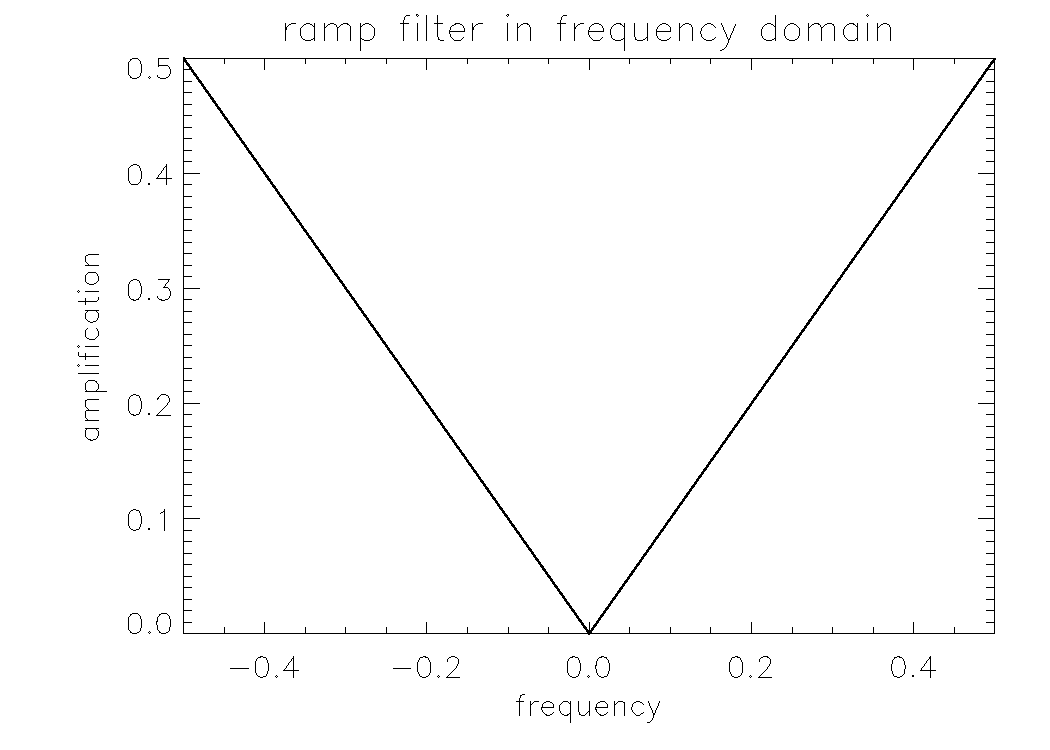
\includegraphics[width=0.45\textwidth]{figs/fig_rampfilter1.pdf}
  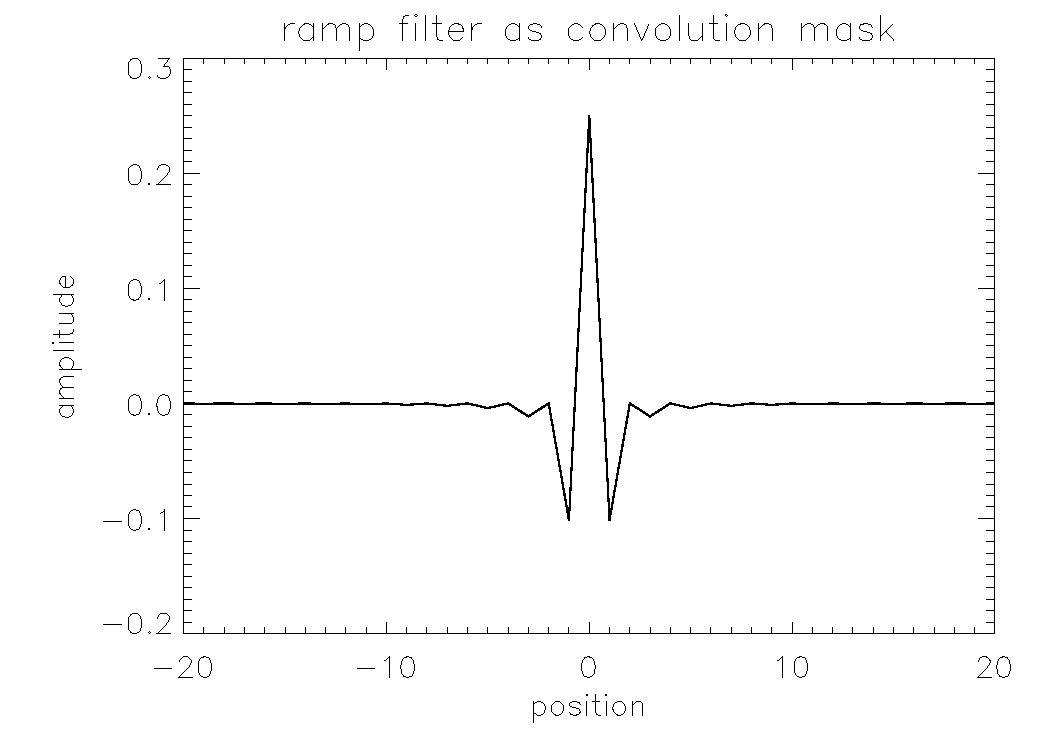
\includegraphics[width=0.45\textwidth]{figs/fig_rampfilter2.pdf}
\caption{\label{fig:rampfilter} \emph{The rampfilter in the frequency
    domain (left) and its point spread function (right). The latter is
    by definition also the mask needed to compute the filter with a
    convolution in the spatial domain.}}
\end{figure}

The ramp filter obviously amplifies high frequencies. If the
projection data are noisy, the reconstructed image will suffer from
high frequency noise. To reduce that noise, filtered backprojection is
always applied in combination with a smoothing (low pass) filter.

\subsubsection{Attenuation correction} \label{sec:attencor}
%------------------------------------
From a CT-measurement, we can directly compute a sinogram of line integrals.
Starting from eq (\ref{eq:ct_proj}) we obtain:
\begin{equation}
  \ln \frac{t_0}{t(b)} = \int_a^b \mu(s) ds. \label{eq:attencor}
\end{equation}
CT measurements have low noise and narrow PSF, so filtered backprojection
produces good results in this case. For emission tomography, the assumptions
are not valid. Probably the most important deviation from the FBP-model is the
presence of attenuation.

Attenuation cannot be ignored. E.g. at 140 keV, every 5 cm of tissue eliminates
about 50\% of the photons. So in order to apply filtered backprojection, we
should first correct for the effect of attenuation. In order to do so, we have
to know the effect. This knowledge can be obtained with a measurement.
Alternatively, we can in some cases obtain a reasonable estimate of that effect
from the emission data only.

In order to measure attenuation, we can use an external radioactive source
rotating around the patient, and use the SPECT or PET system as a CT-camera to
do a transmission measurement. If the external source emits $N_0$ photons
along the x-axis, the expected fraction of photons making it through the
patient is:
\begin{equation}
\frac{N(d)}{N_0} = e^{-\int_a^d \mu(x) dx} \label{eq:ct_proj2}.
\end{equation}
This is identical to the attenuation-factor in the PET-projection, equation
(\ref{eq:pet_proj}). So we can correct for attenuation by multiplying the
emission measurement $q(d)$ with the correction factor $N_0 / N(d)$.
For SPECT (equation (\ref{eq:spect_proj})), this is not possible.

In many cases, we can assume that attenuation is approximately constant (with
known attenuation coefficient $\mu$) within the body contour. Often, we can
obtain a fair body contour by segmenting a reconstruction obtained without
attenuation correction. In that case, (\ref{eq:ct_proj2}) can be computed from
the estimated attenuation image.

Bellini has adapted filtered backprojection for constant SPECT-like attenuation
within a known contour in 1979. The inversion of the general attenuated Radon
transform (i.e. reconstruction for SPECT with arbitrary (but known) attenuation) has
been studied extensively, but only in 2000 Novikov found a solution. The solution
came a bit late in fact, because by then, iterative reconstruction had replaced
analytical reconstruction as the standard approach in SPECT. And in iterative
reconstruction, non-uniform attenuation poses no particular problems.

\subsection{Iterative Reconstruction} \label{sec:iterrecon}
%====================================
Filtered backprojection is elegant and fast, but not very
flexible. The actual acquisition differs considerably from the ideal
projection model, and this deviation causes reconstruction
artifacts. It has been mentioned that attenuation correction in SPECT
may be problematic, but there are other deviations from the ideal line
integral: the measured projections are not continuous but discrete,
they contain a significant amount of noise (Poisson noise), the point
spread function is not a Dirac impulse and Compton scatter may
contribute significantly to the measurement.

That is why many researchers have been studying iterative algorithms. The nice
thing about these algorithms is that they are not based on mathematical
inversion.  All they need is a mathematical model of the acquisition, not its
inverse. Such a forward model is much easier to derive and program. That
forward model allows the algorithm to {\em evaluate} any reconstruction, and
to {\em improve} it based on that evaluation. If well designed, iterative
application of the same algorithm should lead to continuous improvement, until
the result is ``good enough''.

There are many iterative algorithms, but they are rather similar, so
explaining one should be sufficient. In the following, the maximum-likelihood
expectation-maximization (ML-EM) algorithm is discussed, because it is
currently by far the most popular one.

The algorithm is based on a Bayesian description of the problem. In
addition, it assumes that both the solution and the measurement are
discrete. This is correct in the sense that both the solution and the
measurement are stored in a digital way. However, the true tracer
distribution is continuous, so the underlying assumption is that this
distribution can be well described with a discrete representation.

\subsubsection{Bayesian approach} \label{sec:bayes}
%--------------------------------
Assume that somehow we have computed the reconstruction $\Lambda$ from the
measurement $Q$. The likelihood that both the measurement and the
reconstruction are the true ones ($p(Q \; \mbox{and} \; \Lambda)$) can be
rewritten as:
\begin{equation}
  p(\Lambda | Q) p(Q) = p(Q | \Lambda) p(\Lambda).
\end{equation}
It follows that
\begin{equation}
   p(\Lambda | Q) = \frac{p(Q | \Lambda) p(\Lambda)}{p(Q)}. \label{eq:jnpost}
\end{equation}
This expression is known as {\em Bayes' rule}. The function
$p(\Lambda)$ is called {\em the prior}. It is the likelihood of an
image, without taking into account the data. It is only based on
knowledge we already have prior to the measurement. E.g. the
likelihood of a patient image, clearly showing that the patient has no
lungs and four livers is zero. The function $p(Q | \Lambda)$ is simply
called {\em the likelihood} and gives the probability to obtain
measurement $Q$ assuming that the true distribution is $\Lambda$. The
function $p(\Lambda | Q)$ is called {\em the posterior}. The
probability $p(Q)$ is a constant value, since the data $Q$ have been
measured and are fixed during the reconstruction.

Maximizing $p(\Lambda | Q)$ is called the {\em maximum-a-posteriori (MAP)}
approach. It produces ``the most probable'' solution. Note that this doesn't
have to be the true solution. We can only hope that this solution shares
sufficient features with the true solution to be useful for our purposes.

Since it is not trivial to find good mathematical expressions for the prior
probability $p(\Lambda)$, it is often assumed to be constant, i.e.\ it is
assumed that a priori all possible solutions have the same probability to be
correct.  Maximizing $p(\Lambda | Q)$ then reduces to maximizing the
likelihood $p(Q | \Lambda)$, which is easier to calculate.  This is called the
{\em maximum-likelihood (ML)} approach, discussed in the following.

\subsubsection{The likelihood function for emission tomography}
%--------------------------------------------------------------
We have to compute the likelihood $p(Q | \Lambda)$, assuming that the
reconstruction image $\Lambda$ is available and represents the true
distribution. In other words, how likely is it to measure $Q$ with a PET or
SPECT camera, when the true tracer distribution is $\Lambda$?

We start by computing what we would expect to measure. We have already
done that, it is the attenuated projection from equations
(\ref{eq:spect_proj}) and (\ref{eq:pet_proj}). However, we want a
discrete version here:
\begin{equation}
  r_i = \sum_{j=1,J} c_{ij} \lambda_j, \;\; i = 1,I.  \label{jn:mlproj}
\end{equation}
Here, $\lambda_j \in \Lambda$ is the regional activity present in the
volume represented by pixel $j$ (since we have a finite number of
pixels, we can identify them with a single index). The value $r_i$ is
the number of photons measured in detector position $i$ ($i$ combines
the digitized coordinates $(d,\theta,z)$, it identifies a single
projection line). The value $c_{ij}$ represents the sensitivity of
detector $i$ for activity in $j$. If we have good collimation,
$c_{ij}$ is zero everywhere, except for the $j$ that are intersected
by projection line $i$, so the matrix $C$, often called the system
matrix, is very sparse. This notation is very general, and allows us
e.g. to take into account the finite acceptance angle of the
mechanical collimator (which will increase the fraction of non-zero
$c_{ij}$). If we know the attenuation coefficients, we can include
them in the $c_{ij}$, and so on. Consequently, this approach is valid
for SPECT and PET.

We now have for every detector two values: the expected value $r_i$ and the
measured value $q_i$. Since we assume that the data are samples from a Poisson
distribution, we can compute the likelihood of measuring $q_i$, if $r_i$
photons were expected (see eq. (\ref{jn:Poisson})):
\begin{equation}
  p(q_i | r_i) = \frac{e^{-r_i} r_i^{q_i}}{q_i!}.
\end{equation}
The history of one photon (emission, trajectory, possible interaction with
electrons, possible detection) is independent of that of the other photons, so
the overall probability is the product of the individual ones:
\begin{equation}
  p(Q | \Lambda) = \prod_i \frac{e^{-r_i} r_i^{q_i}}{q_i!}. \label{jn:mllik}
\end{equation}

Obviously, this is going to be a very small number: e.g. $p(q_i = 15 | r_i =
15) = 0.1$ and smaller for any other $r_i$. For larger $q_i$, the maximum
$p$-value is even smaller. In a measurement for a single slice, we have in the
order of 10000 detector positions, so the maximum likelihood value may be in
the order of $10^{-10000}$, which is zero in practice. We are {\em sure} the
solution will be wrong. However, we hope it will be close enough to the true
solution to be useful.

Maximizing (\ref{jn:mllik}) is equivalent to maximizing its logarithm, since
the logarithm is monotonically increasing. When maximizing over $\Lambda$,
factors not depending on $\lambda_j$ can be ignored, so we will drop $q_i!$
from the equations. The resulting log-likelihood function is
\begin{eqnarray}
  L(Q | \Lambda) & = & \sum_i q_i \ln(r_i) - r_i \\
        & = & \sum_i q_i \ln(\sum_j c_{ij} \lambda_j) - \sum_j c_{ij}
           \lambda_j. \label{eq:likelihood}
\end{eqnarray}

It turns out that the Hessian (the matrix of second derivatives) is negative
definite if the matrix $c_{ij}$ has maximum rank. In practice, this means that
the likelihood function has a single maximum, provided that a sufficient amount
of different detector positions $i$ were used.

\subsubsection{Maximum-Likelihood Expectation-Maximization}
%----------------------------------------------------------
Since we can compute the first derivative (the gradient), many algorithms can
be devised to maximize $L$. A straightforward one is to set the first
derivative to zero and solve for $\lambda$.
\begin{equation}
 \frac{\partial L}{\partial \lambda_j} = \sum_i c_{ij} \left(
      \frac{q_i}{\sum_k c_{ik} \lambda_k} - 1 \right) = 0, \forall i = 1,I.
       \label{eq:jnmlgrad}
\end{equation}
This produces a huge set of equations, and analytical solution is not
feasible.

Iterative optimization, such as a gradient ascent algorithm, is a suitable
alternative.  Starting with an arbitrary image $\Lambda$, the gradient for
every $\lambda_j$ is computed, and a value proportional to that gradient is
added.  Gradient ascent is robust but can be very slow, so more sophisticated
algorithms have been investigated.

A very nice and simple algorithm with guaranteed convergence is the {\em
expectation- maximization (EM)} algorithm.  Although the resulting algorithm
is simple, the underlying theory is not. In the following we simply state that
convergence is proved and only show what the EM algorithm does. The interested
reader is referred to appendix \ref{app:em} for some notes on convergence.

\paragraph{Expected value of Poisson variables, given a single measurement
 \label{sec:expect_a_b}\\}
%''''''''''''''''''''''''''''''''''''''''''''''''''
The iterative algorithm described below makes use of the expected value of a
Poisson variable that contributes to a measurement. This section shows how
that value is computed. Consider the experiment of
fig \ref{fig:expected_a_b}: two vials containing a known amount of
radioactivity are put in front of a detector.
%
\begin{figure}[tb]
\centering
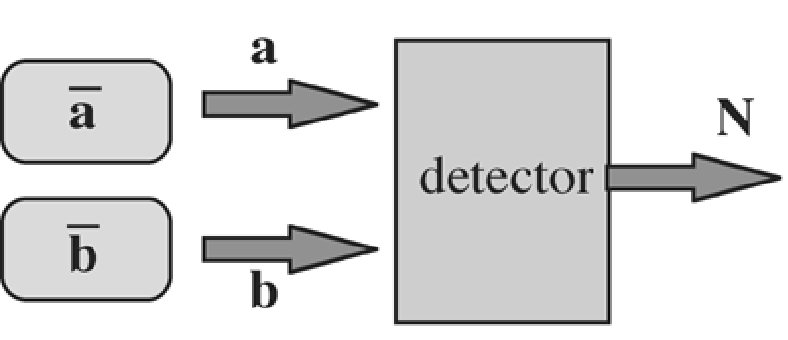
\includegraphics[width=0.4\textwidth]{figs/fig_expected_a_b.pdf}
\caption{\label{fig:expected_a_b} \emph{A detector measures the counts emitted
by two sources.}}
\end{figure}
%
Assume that we know the efficiency of the detector and its sensitivity for the
two vials, so that we can compute the expected amount of photons that each of
the vials will contribute during a measurement. The expected count is
$\bar{a}$ for vial 1 and $\bar{b}$ for vial 2. Now a single experiment is
carried out, and $N$ counts are measured by the detector.  Question: how many
photons $a$ and $b$ were emitted by each of the vials?

A-priori, we would expect $\bar{a}$ photons from vial 1 and $\bar{b}$ photons
from vial 2. But then the detector should have measured $\bar{a} + \bar{b}$
photons. In general, $N \neq \bar{a} + \bar{b}$ because of Poisson noise. So
the measurement $N$ supplies additional information, which we must use to
improve our expectations about $a$ and $b$. The answer is computed in appendix
\ref{app:expected_a_b}. The expected value of $a$, given $N$ is:
\begin{equation}
  E(a | a + b = N) = \bar{a} \frac{N}{\bar{a} + \bar{b}}, \label{eq:expect_a_b}
\end{equation}
and similar for $b$. So if more counts $N$ were measured than the expected
$\bar{a}+\bar{b}$, the expected value of the contributing sources is
``corrected'' with the same factor. Extension to more than two sources is
straightforward.

\paragraph{The complete variables\\}
%''''''''''''''''''''''''''''''''''
To maximize the likelihood (\ref{eq:likelihood}), a trick is applied
which at first seems to make the problem more complicated. We
introduce a so-called set of ``complete'' variables $X = \{ x_{ij}\}$,
where $x_{ij}$ is the (unknown) number of photons that have been
emitted in $j$ and detected in $i$. The $x_{ij}$ are not observable,
but if we would have known them, the observed variables $q_i$ could be
computed, since $q_i = \sum_j x_{ij}$. Obviously, the expected value
of $x_{ij}$, given $\Lambda$ is
\begin{equation}
  E(x_{ij} | \Lambda) =  c_{ij} \lambda_j
\end{equation}
We can now derive a log-likelihood function for the complete variables $X$, in
exactly the same way as we did for $L$ (the $x_{ij}$ obey Poisson
statistics, just as $q_i$). This results in:
\begin{equation}
  L_x(X, \Lambda) = \sum_i \sum_j ( x_{ij} \ln (c_{ij} \lambda_j) - 
                    c_{ij} \lambda_j) \label{eq:jnlx}
\end{equation}
The EM algorithm prescribes a two stage procedure (and guarantees that
applying it repeatedly leads to the maximisation of both $L_x$ and
$L$). It is an iterative algorithm, which starts from a given
image, called $\Lambda^{old}$, and computes an improved image
$\Lambda^{new}$. The two stages are:
\begin{enumerate}
\item Compute the function $E(L_x(X, \Lambda) | Q,
      \Lambda^{old})$. Given $\Lambda^{old}$ and $Q$, it is impossible
      to compute $L_x(X, \Lambda)$, since we don't know the values of
      $x_{ij}$. However, we can calculate its {\em expected} value,
      using the current estimate $\Lambda^{old}$. This is called the
      {\em E-step}.
\item Calculate a new estimate of $\Lambda$ that maximizes the function
      derived in the first step. This is the {\em M-step}.
\end{enumerate}

\paragraph{The E-step\\}
%'''''''''''''''''''''''
The E-step yields the following expressions:
\begin{eqnarray}
E(L_x(X, \Lambda) | Q, \Lambda^{old}) & = & 
   \sum_i \sum_j ( n_{ij} \ln (c_{ij} \lambda_j) -  c_{ij} \lambda_j)
   \label{eq:jnestep1}\\
n_{ij} & = & c_{ij} \lambda_j^{old} \frac{q_i}{\sum_k c_{ik} \lambda_k^{old}}
   \label{eq:jnestep2}
\end{eqnarray}
Equation (\ref{eq:jnestep1}) is identical to equation (\ref{eq:jnlx}), except
that the unknown $x_{ij}$ values have been replaced by their expected values
$n_{ij}$. We would expect that $n_{ij}$ equals $c_{ij}
\lambda_j^{old}$. However, we also know that the sum of all $c_{ij}
\lambda_j^{old}$ equals the number of measured photons $q_i$. This situation
is identical to the problem studied in section \ref{sec:expect_a_b}, and 
equation (\ref{eq:jnestep2}) is the straightforward extension of equation
(\ref{eq:expect_a_b}) for multiple sources.

\paragraph{The M-step\\}
In the M-step, we maximize this expression with respect to $\lambda_j$, by
setting the partial derivative to zero:
\begin{equation}
\frac{\partial}{\partial \lambda_j} E(L_x(X, \Lambda) | Q, \Lambda^{old})
   =  \sum_i \left( \frac{n_{ij}}{\lambda_j} - c_{ij} \right) = 0
\end{equation}
So we find:
\begin{equation}
 \lambda_j  =  \frac{\sum_i n_{ij}}{\sum_i c_{ij}} \label{eq:jnmstep}
\end{equation}
Substitution of equation (\ref{eq:jnestep2}) produces the ML-EM
algorithm:
\begin{equation}
  \lambda_j^{new}  =  \frac{\lambda_j^{old}}{\sum_i c_{ij}}
           \sum_i c_{ij}  \frac{q_i}{\sum_k c_{ik} \lambda_k^{old}}
           \label{eq:jnmlem}
\end{equation}

\paragraph{Discussion\\}

This equation has a simple intuitive explanation:
\begin{enumerate}
\item
The ratio $q_i / \sum_j c_{ij} \lambda_j^{old}$ compares the measurement to
its expected value, based on the current reconstruction. If the ratio is
1, the reconstruction must be correct. Otherwise, it has to be improved.

\item
The ratio-sinogram is backprojected. The digital version of the backprojection
operation is
\begin{equation}
  \mbox{backprojection of $f$ equals: } b_j = \sum_i c_{ij} f_i.
\end{equation}
We have seen the continuous version of the backprojection in
(\ref{eq:jnbackproj}). The digital version clearly shows that
backprojection is the transpose (or the adjoint) of projection
\footnote{The adjoint of a matrix is its conjugate transpose. Because
  the projection coefficients are real values, the adjoint of the
  projection matrix is its transpose.}
: the operations are identical, except that backprojection sums over $i$,
while projection sums over $j$. Note that if the projection takes
attenuation into account, the backprojection does so to. The
backprojection does not attempt to correct for attenuation (it is not
the inverse), it simply applies the same attenuation factors as in the
forward projection.

\item
Finally, the backprojected image is normalized and multiplied with the current
reconstruction image.  It is clear that if the measured and computed sinograms
are identical, the entire operation has no effect. If the measured projection
values are higher than the computed ones, the reconstruction values tend to
get increased.
\end{enumerate}

If the initial image is non-negative, then the final image will be
non-negative too, since all factors are non-negative. This is in most
applications a desirable feature, since the amount of radioactivity
cannot be negative.

Comparing with (\ref{eq:jnmlgrad}) shows that the ML-algorithm is really a
gradient ascent method. It can be rewritten as
\begin{equation}
 \lambda_j^{\mbox{new}} = \lambda_j 
    + \frac{\lambda_j}{\sum_i c_{ij}} \frac{\partial L}{\partial \lambda_j}.
\end{equation}
So the gradient is weighted by the current reconstruction value, which is
guaranteed to be positive (negative radioactivity is meaningless). To make it
work, we can start with any non-zero positive initial image, and iterate until
the result is ``good enough''. Fig. \ref{fig:jnfbpml} shows the filtered
backprojection and ML-EM reconstructions from the same dataset. (The image
shown is not the true maximum likelihood image, since iterations were stopped
early as discussed below).
\begin{figure}[tb]
\centering
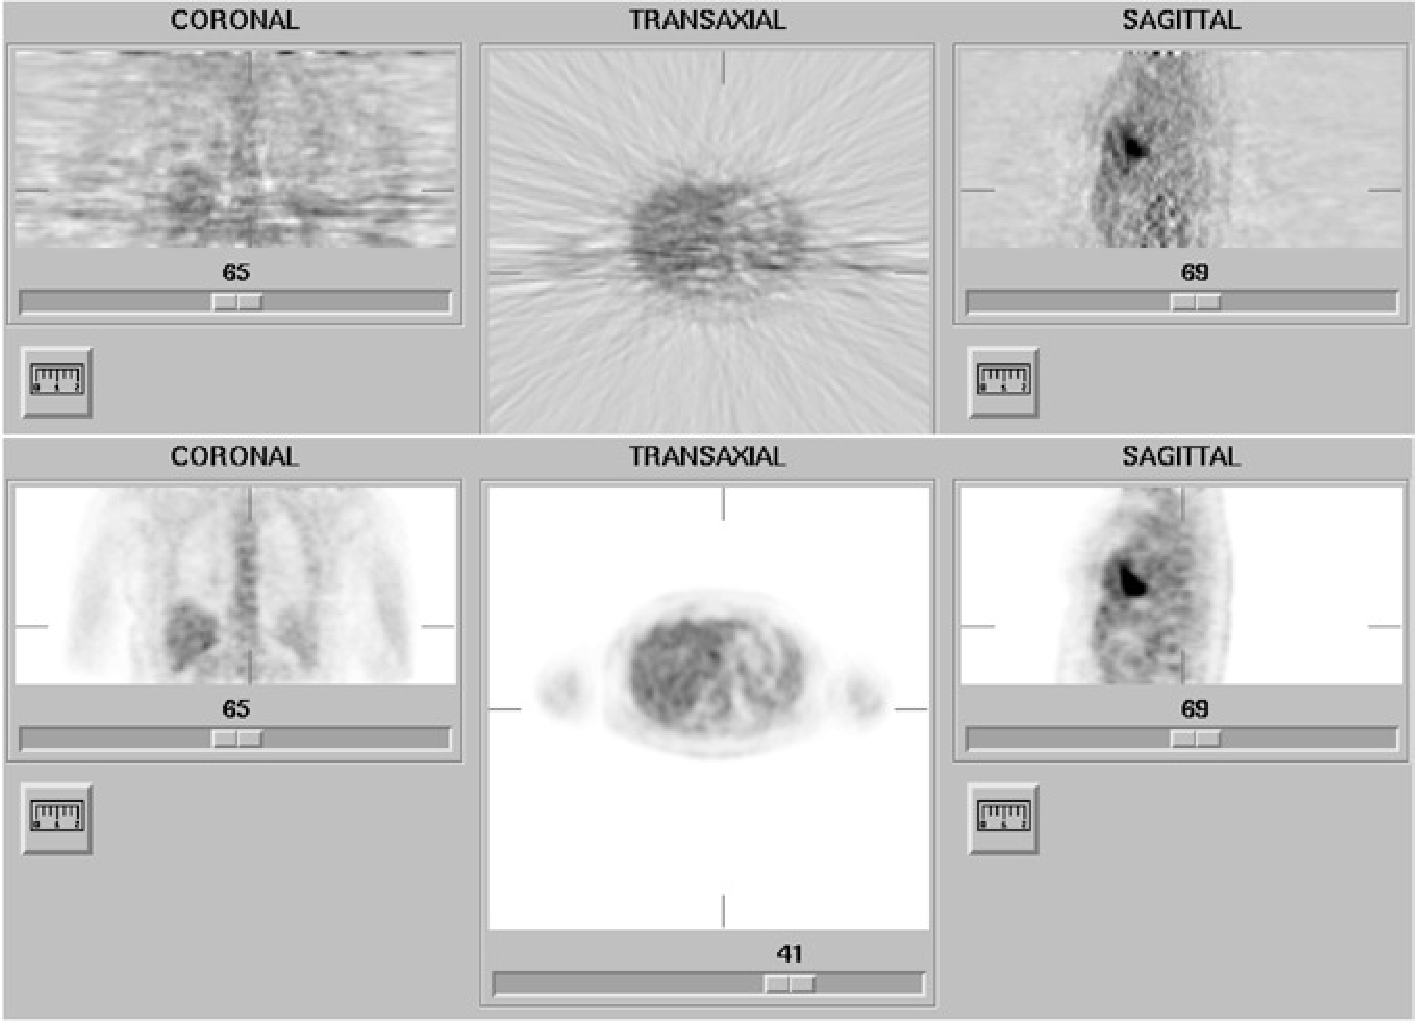
\includegraphics[width=0.72\textwidth]{figs/fig_jnfbpml.pdf}
\caption{\label{fig:jnfbpml} \emph{Reconstruction obtained with filtered
backprojection (top) and maximum-likelihood expectation-maximization (34
iterations) (bottom). The streak artifacts in the filtered backprojection
image are due to the statistical noise on the measured projection (Poisson
noise).}}
\end{figure}

\subsection{Compton scatter, random coincidences}
%================================================
As explained in section \ref{sec:randoms}, an estimate of the randoms
contribution to the PET sinogram can be obtained, e.g. with the
delayed window technique. Similarly, various methods exist to estimate
the scatter contribution in SPECT (section \ref{sec:spectscatcor})
and PET (section \ref{sec:petscatcor}). If an estimate of such an
additive contribution to the sinogram is available, it can be
incorporated in the ML-EM algorithm. The forward acquisition model
of (\ref{jn:mlproj}) is then extended as 
\begin{equation}
  r_i = \sum_{j=1,J} c_{ij} \lambda_j + s_i, \;\; i = 1 \ldots I,
  \label{jn:mlprojscat}
\end{equation}
where $s_i$ represents the estimate of the additive contribution from
scatter and/or randoms for projection line $i$. It can be shown that
the ML-EM algorithm then becomes
\begin{equation}
  \lambda_j^{new}  =  \frac{\lambda_j^{old}}{\sum_i c_{ij}}
           \sum_i c_{ij}  \frac{q_i}{\sum_k c_{ik} \lambda_k^{old} + s_i}
           \label{eq:jnmlemscat}
\end{equation}



\subsection{Regularization} \label{sec:regularization}
%==========================
Since the levels of radioactivity must be low, the number of detected photons
is also low. As a result, the uncertainty due to Poisson noise is important:
the data are often very noisy. 

Note that Poisson noise is ``white''. This means that its (spatial) frequency
spectrum is flat. Often this is hard to believe: one would guess it to be high
frequency noise, because we see small points, no blobs or a shift in mean
value.  That is because our eyes are very good at picking up high frequencies:
the blobs and the shift are there all right, we just don't see them.

Filtered backprojection has not been designed to deal with Poisson
noise. The noise propagates into the reconstruction, and in that
process it is affected by the ramp filter, so the noise in the
reconstruction is not white, it is truly high frequency noise. As a
result, it is definitely {\em not} Poisson noise. Figure
\ref{fig:jnfbpml} clearly shows that Poisson noise leads to streak
artifacts when filtered backprojection is used.

ML-EM does ``know'' about Poisson noise, but that does not allow it to separate
the noise from the signal. In fact, MLEM attempts to compute how many of the
detected photons have been emitted in each of the reconstruction pixels
$j$. That must produce a noisy image, because photon emission is a Poisson
process. What we really would like to know is the tracer concentration, which
is not noisy.

Because our brains are not very good at suppressing noise, we need to
do it with the computer. Many techniques exist. One can apply simple
smoothing, preferably in three dimensions, such that resolution is
approximately isotropic. It can be shown that for every isotropic 3D
smoothing filter applied after filtered backprojection, there is a 2D
smoothing filter, to be applied to the measured data before filtered
backprojection, which has the same effect. Since 2D filtering is
faster than 3D filtering, it is common practice to smooth before
filtered backprojection.

The same is not true for ML-EM: one should not smooth the measured projections,
since that would destroy the Poisson nature. Instead, the images are often
smoothed afterwards. Another approach is to stop the iterations before
convergence. ML-EM has the remarkable feature that low frequencies converge
faster than high ones, so stopping early has an effect similar to low-pass
filtering.

Finally, one can go back to the basics, and in particular to the
Bayesian expression (\ref{eq:jnpost}). Instead of ignoring the prior,
one can try and define some prior probability function that encourages
smooth solutions. This leads to maximum-a-posteriori (MAP)
algorithm. The algorithms can be very powerful, but they also have
many parameters and tuning them is a delicate task.

Although regularized (smoothed) images look much nicer than the original ones,
they do not contain more information. In fact, they contain less information,
since low-pass filtering kills high-frequency information and adds nothing
instead! Deleting high spatial frequencies results in poorer resolution (wider
point spread function), so excessive smoothing is ill advised if you hope to
see small structures in the image.

\subsection{Convergence} \label{sec:mlemconverge}
%==========================
\begin{figure}[tb]
\centering
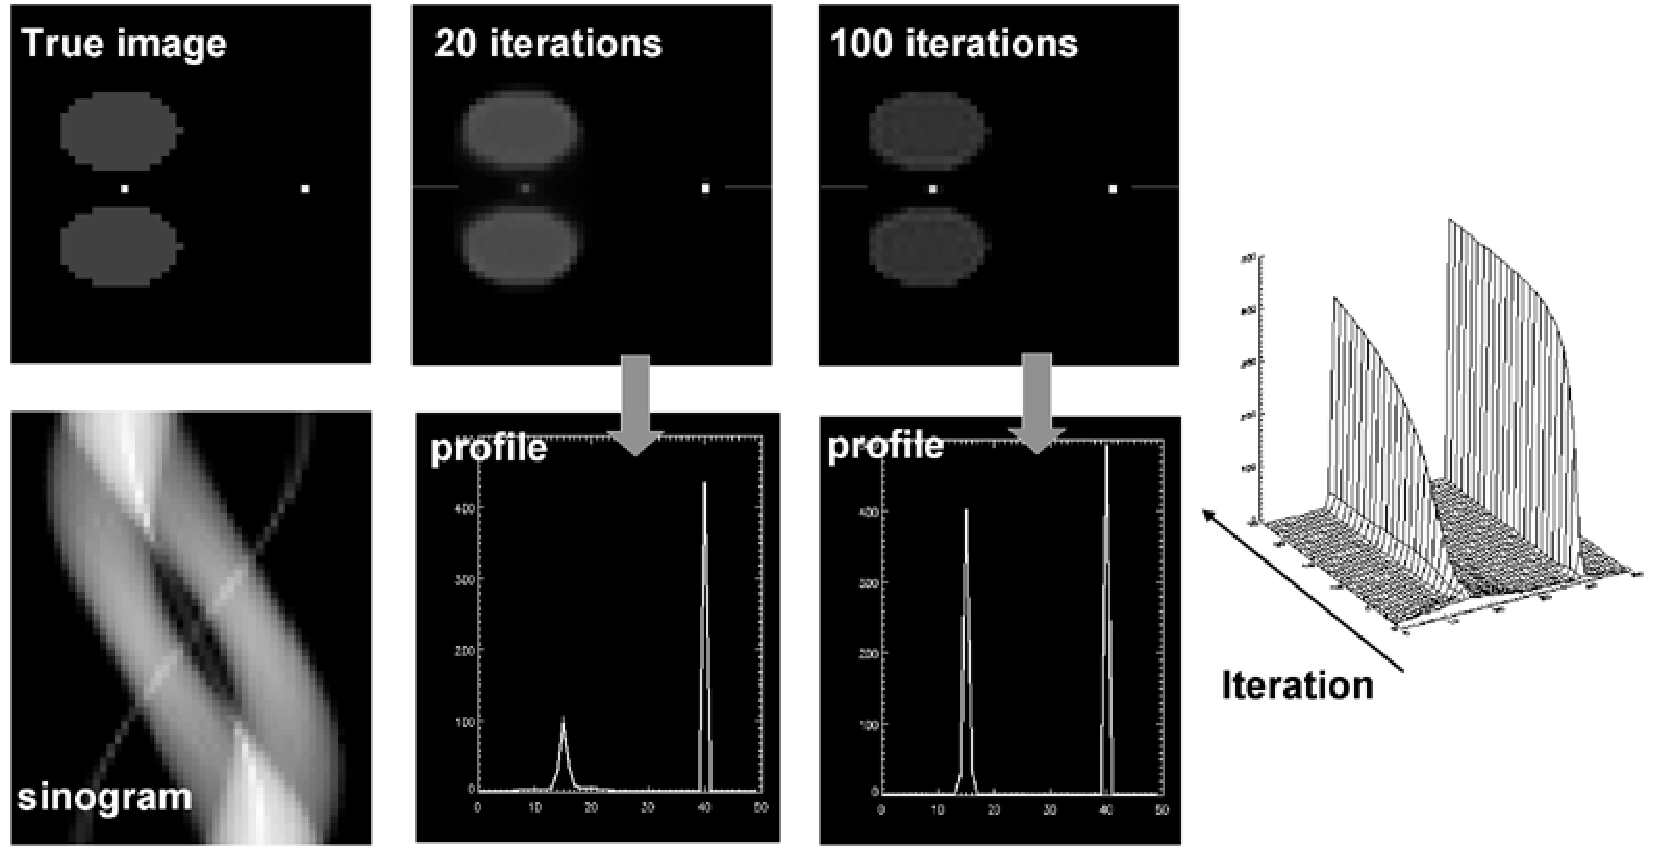
\includegraphics[width=0.9\textwidth]{figs/fig_mlem_converge.pdf}
\caption{\label{fig:mlem_converge} \emph{Simulation designed to challenge
convergence of MLEM: the point between the hot regions convergence very slowly
relative to the other point. The maximum converges slower than the width, so
counts are not preserved.}}
\end{figure}
%
Filtered backprojection is a linear algorithm with shift invariant point
spread function. That means that the effect of projection followed by filtered
backprojection can be described with a single PSF, and that the reconstruction
has a predictable effect on image resolution. Similarly, smoothing is linear
and shift invariant, so the combined effect of filtered backprojection with
low pass filtering has a known effect on the resolution.

In contrast to FBP, MLEM algorithm is non-linear and not shift invariant.
Stated otherwise, if an object is added to the reconstruction, then the effect
of projection followed by reconstruction is different for {\em all} objects in
the image. In addition, two identical objects can be reconstructed differently
because they are at a different position. In this situation, it is impossible
to define a PSF, projection followed by MLEM-reconstruction cannot be modeled
as a convolution. There is no easy way to predict the effect of MLEM on image
resolution. 

It is possible to predict the resolution of the true maximum likelihood
solution, but you need an infinite number of iterations to get
there. Consequently, if iterations are stopped early, convergence may be
incomplete. There is no way to tell that from the image, unless you knew
a-priori what the image was: MLEM images always look nice. So stopping
iterations early in patient studies has unpredictable consequences.

This is illustrated in a simulation experiment shown in figure
\ref{fig:mlem_converge}. There are two point sources, one point source is
surrounded by large active objects, the other one is in a cold region. After
20 MLEM iterations, the ``free'' point source has nearly reached its final
value, while the other one is just beginning to appear. Even after 100
iterations there is still a significant difference. The difference in
convergence affects not only the maximum count, but also the total count in a
region around the point source.

Consequently, it is important to apply ``enough'' iterations, to get
``sufficiently'' close to the true ML solution. In the previous section it was
mentioned that stopping iterations early has a noise-suppressing effect. 
%
\begin{figure}[tb]
\centering
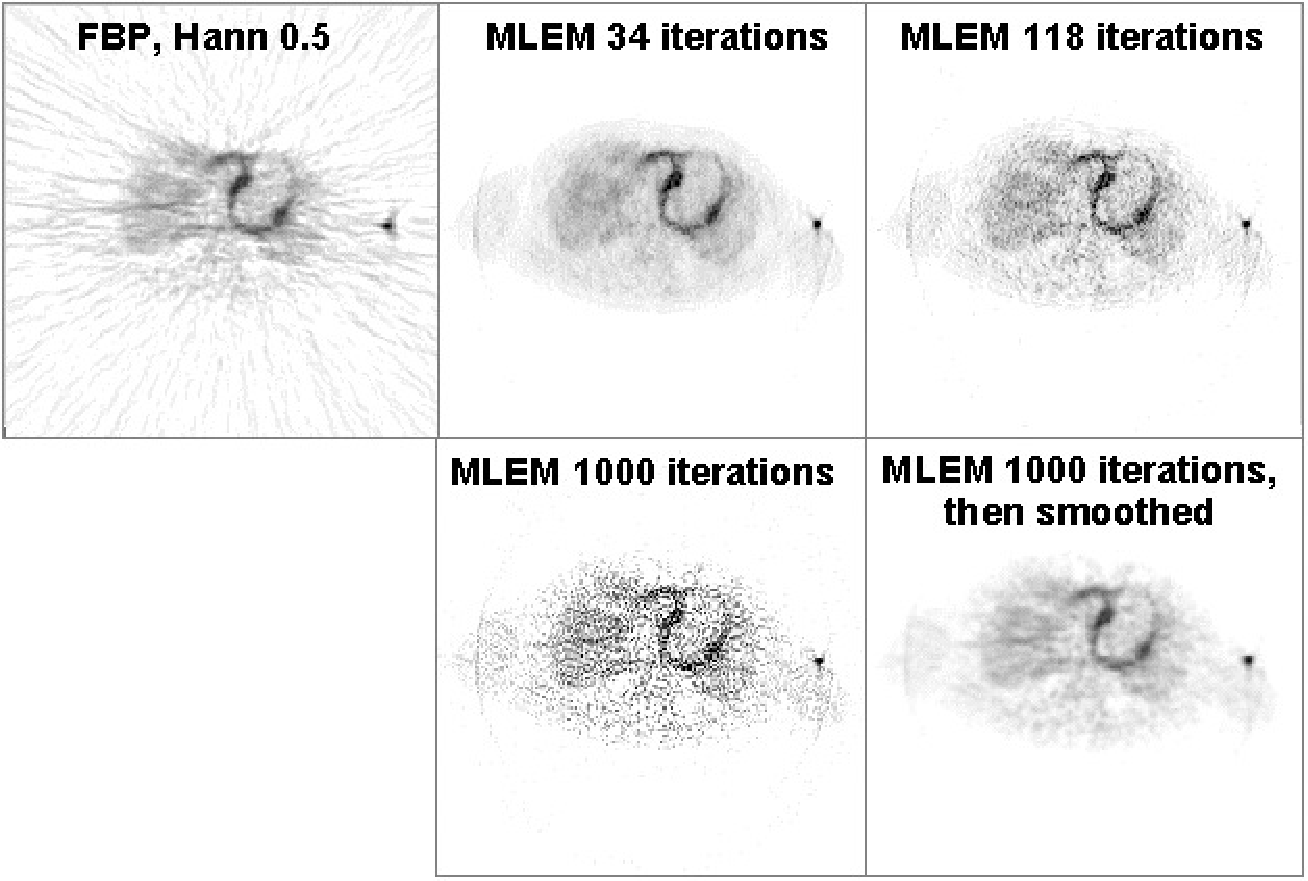
\includegraphics[width=0.9\textwidth]{figs/fig_mlem_1000iter.pdf}
\caption{\label{fig:mlem_1000iter} \emph{Reconstruction of a cardiac PET scan
with FBP, and with MLEM. The images obtained after 34, 118 and 1000 iterations
are shown. The image at 1000 iterations is very noisy, but a bit of smoothing
turns it into a very useful image.}}
\end{figure}
%
This is illustrated in figure \ref{fig:mlem_1000iter}. After 34 MLEM
iterations a ``nice'' image is obtained. After 1000 iterations, the image is
very noisy. However, this noise is highly correlated, and drops dramatically
after a bit of smoothing (here with a Gaussian convolution mask). 

From figures \ref{fig:mlem_converge} and \ref{fig:mlem_1000iter} it follows
that it is better to apply many iterations and remove the noise afterwards
with post-smoothing. In practice, ``many'' is at least 30 iterations for
typical SPECT and PET images, but for some applications it can mean several
hundreds of iterations. One finds that when more effects are included in
the reconstruction (such as attenuation, collimator blurring, scatter,
randoms...), more iterations are needed.  The number also depends on the image
size, more iterations are needed for larger images. So if computer time is not
a problem, it is recommended to apply really many iterations (several
hundreds) and regularize with a prior or with post-smoothing.

\subsection{OSEM} \label{sec:osem}
%==========================
\begin{figure}[tb]
\centering
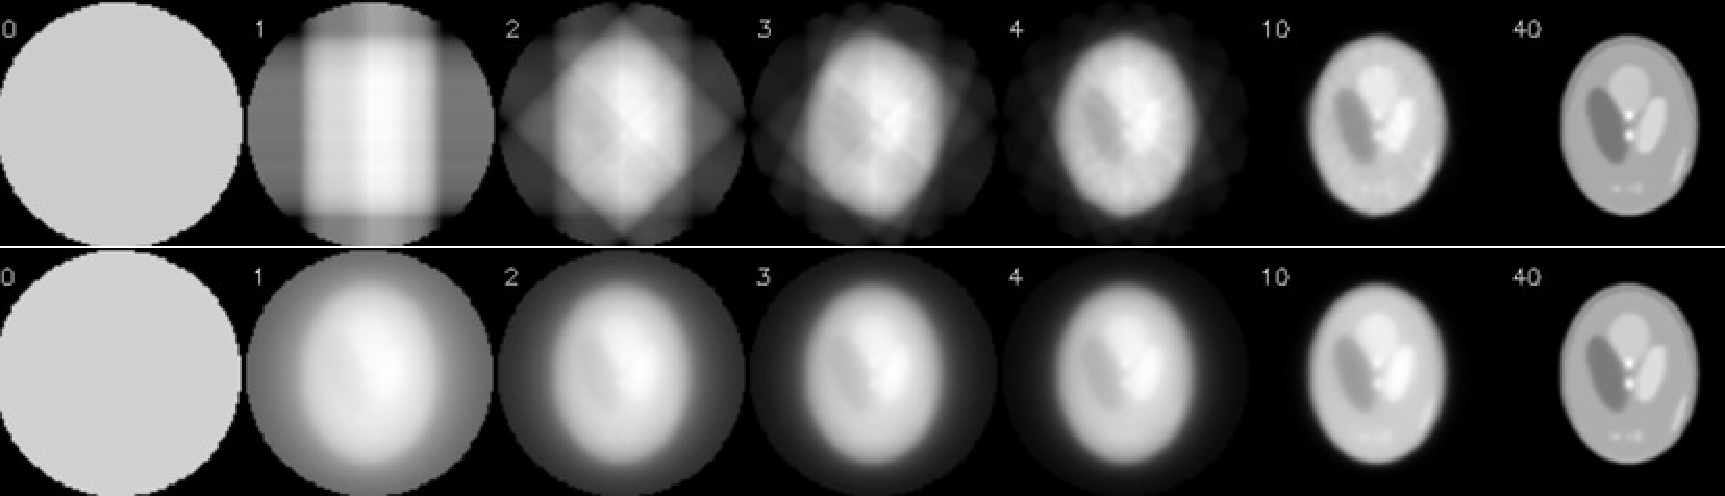
\includegraphics[width=\textwidth]{figs/fig_osem.pdf}
\caption{\label{fig:osem} \emph{Illustration of OSEM: there are 160
    projections in the sinogram, for an acquisition over
    360\textdegree. OSEM used 40 subsets of 4 projections each, the first
    subset has projections at 0\textdegree, 90\textdegree, 180\textdegree and
    270\textdegree. The second subset starts at 45\textdegree and so on. One
    OSEM iteration has 40 subiterations. The top row shows the first
    few and the last subiteration of OSEM. The bottom row shows the
    corresponding MLEM-iterations, where all projections are used for
    each iteration.}}
\end{figure}
In each iteration, MLEM must compute a projection and a
backprojection, which is very time consuming. FBP is much faster, it
uses only a single backprojection, the additional cpu-time for the
ramp filtering is small. Consequenly, the computation of 30 MLEM
iterations takes about 60 times longer than an FBP
reconstruction. MLEM was invented by Shepp and Vardi in 1982, but the
required cpu time prohibited application in clinical routine. Only
after 1992 clinical application started, partly because the computers
had become more powerful, and partly because a very simple
acceleration trick was proposed by Hudson and Larkin. The trick is
called ``ordered subsets expectation maximisation (OSEM)'', and the
basic idea is to use only a part of the projections in every
ML-iteration. This is illustrated in fig \ref{fig:osem}. In this
example, there are 160 projections, which are divided in 40 subsets of
4 projections per subset. The first subset contains the projections
acquired at 0\textdegree, 90\textdegree, 180\textdegree and 270\textdegree. The
second subset has the projections at 45\textdegree, 135\textdegree,
225\textdegree and 315\textdegree and so on. One OSEM iteration consists of
40 subiterations. In the first subiteration, the projection and
backprojection is restricted to the first subset, the second
subiteration only uses the second subset and so on. After the last
subiteration, all projections have been used once. As shown in fig
\ref{fig:osem}, 1 OSEM iteration with 40 subsets produces an image
very similar to that obtained with 40 MLEM iterations. Every MLEM
iteration uses all projections, so in this example, OSEM obtains the
same results 40 times faster.

A single OSEM iteration can be written as
\begin{equation}
  \lambda_j^{new}  =  \frac{\lambda_j^{old}}{\sum_{i\in S_k} c_{ij}}
           \sum_{i\in S_k} c_{ij}  \frac{q_i}{\sum_j c_{ij} \lambda_j^{old}},
           \label{eq:osem}
\end{equation}
where $S_k$ is subset $k$. Usually, one chooses the subsets such that
every projection is in exactly one subset.

The characteristics of OSEM have been carefully studied, both
theoretically and in practice. In the presence of noise, it does not
converge to a single solution, but to a so-called limit cycle. The
reason is that the noise in every subset is different and
``incompatible'' with the noise in the other subsets. As a result,
every subset asks for a (slightly) different solution, and in every
subiteration, the subset in use ``pulls'' the image towards its own
solution. More sophisticated algorithms with better or even guaranteed
convergence have been proposed, but because of its simplicity and good
performance in most cases, OSEM is now by far the most popular
ML-algorithm on SPECT and PET systems.



\section{Fully 3D Tomography}
%%%%%%%%%%%%%%%%%%%%%%%%%%%%%
Until now, we have only discussed the reconstruction of a single 2D slice from
a set of 1D projection data. An entire volume can be obtained by
reconstructing neighboring slices.  This is what happens in SPECT with
parallel hole or fan beam collimation, in 2D PET and in single slice CT.

In some configurations this approach is not possible and the problem
has to be treated as a fully three-dimensional one. There are many
different geometries of mechanical collimators, and some of these
acquire along lines that cannot be grouped in parallel sets. Examples
are the cone beam and pinhole collimators in SPECT (fig
\ref{fig:collimators}). Another example is 3D PET (section
\ref{sec:2D3DPET}). Three approaches to fully 3D reconstruction are
discussed below.

Note that the terminology may create some confusion about the
dimensions. 2D PET actually generates 3D sinogram data: the dimensions
are the detector and the projection angle (defining the projection
line within one slice), and the position of slice. Fully 3D PET
produces 4D sinogram data. The PET detector covers typically a
cylindrical surface. Two coordinates are needed to identify a single
detector, hence four coordinates are needed to identify a projection
line between a pair of detectors. And as will be discussed later, a series
of images can be acquired over time (dynamic acquisitions), which adds
another dimension to the data.


\subsubsection{Filtered backprojection}
%---------------------------------------
Filtered backprojection can be extended to the fully 3D PET case. The data are
backprojected along their detection lines, and then filtered to undo the
blurring effect of backprojection. This is only possible if the sequence of
projection and backprojection results in a shift-invariant point spread
function. And that is only true if every point in the reconstruction volume is
intersected by the same configuration of measured projection lines.

This is often not the case in practice. Points near the edge of the field of
view are intersected by fewer measured projection lines. In this case, the
data may be completed by computing the missing projections as follows. First a
subset of projections that meets the requirement is selected and reconstructed
to compute a first (relatively noisy) reconstruction image. Next, this
reconstruction is forward projected along the missing projection lines, to
compute the missing data. Then, the computed and measured data are combined
into a single set of data, that now meets the requirement of shift-invariance.
Finally, this completed data set is reconstructed with 3D filtered
backprojection.

\subsubsection{ML-EM reconstruction}
%-----------------------------------
ML-EM can be directly applied to the 3D data set: the formulation is very
general, the coefficients $c_{ij}$ in (\ref{eq:jnmlem}) can be directly used
to describe fully 3D projection lines.

In every iteration, we have to compute a projection and a backprojection along
every individual projection line. As a result, the computational burden may
become pretty heavy for a fully 3D configuration.


\subsubsection{Fourier rebinning}
%--------------------------------
In PET, a rebinning algorithm is an algorithm that resamples the data
in the sinogram space, so as to reorganize them into a form that
leads to a simpeler reconstruction.
%
In 1997, an exact rebinning algorithm, called {\em Fourier rebinning},
was derived. It converts a set of 3D data into a set of 2D
projections. Because all photons acquired in 3D are used to compute
the rebinned 2D data set, the noise in this data set is much lower
than in the corresponding 2D subset, which is a part of the original
3D data.

These projections can be reconstructed with standard 2D filtered
backprojection.  It was also shown that the Poisson nature of the data
is more or less preserved.  Consequently, the resulting 2D set can be
reconstructed successfully with the 2D ML-EM algorithm as
well. (Fourier rebinning is based on a wonderful feature of the
Fourier transform of the sinograms, hence its name.)

In practice, the exact rebinning algorithm is not used. Instead, one
only applies an approximate expression derived from it, because it is
much faster and sufficiently accurate for most configurations. This
algorithm (called FORE) is available on all commercial PET systems.

\section{Time-of-flight PET} \label{sec:TOF}
%%%%%%%%%%%%%%%%%%%%%%%%%%%%%
The speed of light is c = 30 cm/ns. Suppose that a point source is put
exactly in the center between two PET detectors, which are connected
to coincidence electronics. If two photons from the same annihilation
are detected, then they must have arrived simultaneously in the
respective detectors. However, the timing will be different if the
source is moved 15 cm towards one detector. The photon will arrive in
that detector 0.5 ns earlier, the other photon will arrive in the
other detector 0.5 ns later. Consequently, if the electronics can
measure the difference in arrival times $\Delta t$, then the position
of the annihilation along the projection line can be deduced: $\Delta
R = c \Delta t / 2$, where $\Delta R$ is the distance to the
center. Using this principle in PET is called time-of-flight PET or
TOF-PET.

In the eighties, TOF-PET scanners were built, but their performance
was disappointing. To obtain a reasonable TOF resolution, one needs to
measure the arrival time very accurately. Consequently, crystal
detectors with a very short scintillation time must be used. Such
crystals were available (e.g. CsF), but these fast crystals all had a
poor stopping power (low attenuation coefficient) at 511
keV. Consequently, the gain obtained from the TOF-principle was more
than offset by the loss due to the decreased detection
sensitivity. For that reason, TOF was abandoned, and nearly all
commercial PET scanners were built using BGO, which has a very high
stopping power but a long scintillation time (see table
\ref{tab:crystals}).

More recently, new scintillation crystals have been found, which
combine high stopping power with fast scintillation decay (table
\ref{tab:crystals}). In current scanners, LSO (or LYSO) is mostly
used. And since the eighties, the electronics have become faster as
well. The current commercial TOF-PET systems have a TOF resolution
ranging from around 500 ps (7.5 cm) for older systems to around 200 ps
for new systems (new in 2020).

\begin{figure}[t]
\centering
  \includegraphics[width=0.72\textwidth]{figs/fig_tofsino.pdf}
  \vspace{-4mm}
  \caption{\label{fig:tofsino} \emph{A single plane from a clinical
  TOF-data set, sampled at 13 TOF-bins. The first bin corresponds to
  the center, the subsequent bins are for increasing distances,
  alternatedly in both directions. The non-TOF sinogram was obtained
  by summing the 13 TOF-sinograms.}}
\end{figure}
TOF-PET sinograms (or projections) have one dimension more than the
corresponding non-TOF data, because with TOF, the position along the
projection line is estimated as well. Figure \ref{fig:tofsino} shows a
TOF sinogram (sampled at 13 TOF-bins) together with the non-TOF
sinogram (obtained by adding all TOF-bins).

Consequently, a parallel projection of a 2D image along a single
projection angle, is not a 1D profile but a 2D image. This projection
can be considered as a blurred version of the original image, where
the blurring represents the uncertainty due to the point spread
function of the TOF-position measurement. This can be well modeled as
a 1D Gaussian blurring, as illustrated in fig \ref{fig:TOFproj}.
\begin{figure}[tb]
\centering
  \includegraphics[width=0.7\textwidth]{figs/fig_TOF_projbproj.pdf}
  \caption{\label{fig:TOFproj} \emph{Left: TOF-PET projection (matrix
  A) can be considered as a 1D smoothing along the projection
  angle. Right: the TOF-PET backprojection of TOF-PET projection is
  equivalent to a 2D blurring filter. The blurring is much less than
  in the non-TOF case (fig \ref{fig:backproj}).}}
\end{figure}


For iterative reconstruction, one will need the corresponding
backprojection operator. Using the discrete representation, the
projection can be written as:
\begin{equation}
  q_i = \sum_j c_{ij} \lambda_j,
\end{equation}
which is the same expression as for non-TOF-PET and SPECT
(eq. \ref{jn:mlproj}), but of course, the elements $c_{ij}$ of the
system matrix are different. The corresponding backprojection is then
given by
\begin{equation}
  b_j = \sum_i c_{ij} q_i.
\end{equation}
The transpose of a symmetrical blurring operator is the same blurring
operator. Consequently, every TOF-projection image must be blurred
with its own 1D blurring kernel, and then they all have to be summed
to produce the backprojection image. The PSF of projection followed by
backprojection then yields a circularly symmetrical blob with central
profile
\begin{equation}
  b(r) = \mbox{Gauss}(r,\sqrt{2}\sigma) \frac{1}{|r|}, \label{eq:TOFpsf}
\end{equation}
where $r$ is the distance to the center of the blob, $\sigma$ is the
standard deviation of the Gaussian blurring that represents the TOF
resolution, and Gauss($r,s$) is a Gaussian with standard deviation
$s$, evaluated in $r$. The standard deviation in (\ref{eq:TOFpsf}) is
$\sqrt{2}\sigma$ and not simply $\sigma$, because the blurring has
been applied twice, once during projection and once during
backprojection. See appendix \ref{app:bprojproj} for a more
mathematical derivation.

For very large $\sigma$, this reduces to $b(r) = 1 / |r|$, which is
the result for backprojection in non-TOF PET, obtained just after eq
(\ref{eq:bprojvalue}). The projection and backprojection operators
are illustrated in fig \ref{fig:TOFproj}.

Also for TOF-PET, filtered backprojection algorithms can be
developed. Because of the data redundancy, different versions of FBP
can be derived. A natural choice is to use the same backprojector as
mentioned above. With this backprojector, the backprojection of the
TOF-PET measurement of a point source will yield the image of blob
given by eq (\ref{eq:TOFpsf}). Consequently, the reconstruction filter
can be obtained by computing the inverse operator of
(\ref{eq:TOFpsf}). As before, the filter can be applied before
backprojection (in the sinogram) or after backprojection (in the
image), because of the Fourier theorem.

\begin{figure}[tb]
\centering
\includegraphics[width=0.9\textwidth]{figs/fig_TOF_matej.pdf}
\caption{\label{fig:TOFmatej} \emph{CT and TOF-PET image, acquired on
    a PET/CT system with time-of-flight resolution of about 700
    ps. The TOF-PET image reveals a small lesion not seen on the
    non-TOF PET image. (Courtesy Joel Karp and Samuel Matej,
    University of Pennsylvania. The image is acquired on a Philips
    Gemini TOF-PET system)}}
\end{figure}

Figure \ref{fig:TOFmatej} compares a TOF and non-TOF image. By
discarding the TOF-information, TOF-PET data can be converted to
regular PET data. This was done here to illustrate the improvement
obtained by using TOF. There are several reasons why the TOF-PET image
is better.

First, because more information is used during reconstruction, the
noise propagation is reduced, resulting in a better signal-to-noise
ratio (less noise for the same resolution) in the TOF image. It has
been shown that, for the center of a uniform cylinder, improving the
TOF resolution with a factor reduces the variance in the reconstructed
image with that same factor, at least if these images have the same
spatial resolution.

Second, it turns out that the convergence of the MLEM algorithm is
considerably faster for TOF-PET. It is known that MLEM converges
faster for smaller images, because the correct reconstruction of a
pixel depends on the reconstruction of all other pixels that share
some projection lines with it. The TOF information reduces that number
of information-sharing pixels considerably. Because in clinical
routine, usually a relatively low number of iterations is applied,
small image detail (high spatial frequencies) may suffer from
incomplete convergence. It was found that after introducing TOF, the
spatial resolution of the clinical images was better than before. TOF
has no direct effect on the spatial resolution, but for a similar
number of iterations, MLEM converges faster, producing a better
resolution. And because of the improved SNR, it can achieve this
better resolution at a similar or better noise level than non-TOF
PET. 

Third, an additional advantage of this reduced dependency on other
pixels is a reduced sensitivity to most things that may cause
artifacts, such as errors in the attenuation map, patient motion, data
truncation and so on. In non-TOF PET, the resulting artifacts can
propagate through the entire image. In TOF-PET, that propagation is
reduced because of the reduced dependencies between the reconstructed
pixel values.

Finally, the gain due to TOF is higher when the region of interest is
surrounded by more activity and if the active object (i.e. the patient
body) is larger. The reason is that in those cases, there is more to
be gained by suppressing sensitivity to surrounding activity, since
there is more surrounding activity. As a result, TOF helps more in
situations where non-TOF MLEM performs poorest. The opposite is also
true, for imaging a point source, TOF-PET does not better than non-TOF
PET.

%%%%%%%%%%%%%%%%%%%%%%%%%%%%%
\section{Reconstruction with resolution modeling} \label{sec:resol}
%%%%%%%%%%%%%%%%%%%%%%%%%%%%%
In every MLEM iteration a projection and backprojection is
executed. The projection $\sum_j c_{ij} \lambda_j$ simulates the
acquisition and the backprojection $\sum_i c_{ij} q_i$ is the
corresponding adjoint operator. A more accurate simulation of the
acquisition should result in a more accurate reconstruction of the
image from the acquired tomographic data. In SPECT, the system matrix
elements $c_{ij}$ should account for the position dependent
attenuation to ensure that MLEM produces quantitative images. In PET,
the elements $c_{ij}$ should model the attenuation and detector
sensitivities (see equation \ref{eq:petnorm}), and for TOF-PET, also
the width of the TOF-resolution.

\begin{figure}[htb]
\centering
\includegraphics[width=0.9\textwidth]{figs/fig_resol_line_cone.pdf}
\caption{\label{fig:resolcone} \emph{In a simple projector/backprojector,
    the projection is modeled as a (weighted) line integral. To
    account for the position dependent collimator blurring, the line
    integral can be replaced by a weighted integral over a cone.}}
\end{figure}
In section \ref{sec:collimation}, we have seen that gamma cameras
suffer from position dependent collimator blurring. As illustrated in
figure \ref{fig:resolcone}, this can be modeled by computing the
projection not as a line integral, but as the integral over a cone,
using appropriate weights to model the position dependent PSF. This
position dependent blurring is then combined with the attenuation to
obtain the system matrix elements $c_{ij}$. The same can be done for
PET: the blurring due to the detector width (and if desired, also the
positron range and/or the acolinearity) can be incorporated in the PET
or TOF-PET system matrix elements.

During the iterations, MLEM (or OSEM) uses the system matrix in every
projection and backprojection, and by doing so, it will attempt to
invert all effects modeled by that system matrix. If the system matrix
models a blurring effect, then MLEM will automatically attempt to undo
that blurring. This produces images with improved resolution as
illustrated for a SPECT and a PET case in figure
\ref{fig:resolspectpet}. Interestingly, modeling the finite system
resolution in MLEM not only improves the resolution in the
reconstructed image, it also suppresses the noise, as can be seen in
the PET reconstruction.

\begin{figure}[htb]
\centering
\includegraphics[width=0.9\textwidth]{figs/fig_resol_spectpet.pdf}
\caption{\label{fig:resolspectpet} \emph{Reconstructions with and
    without resolution modeling from a SPECT bone scan of a child and
    a brain PET scan. ``MIP'' denotes ``maximum intensity
    projection''.  MLEM with resolution modeling recovers image detail
    that was suppressed by the finite system resolution.}}
\end{figure}

However, the deblurring cannot be 100\% successful, because deblurring
is a very ill-posed problem. Except in special cases, deblurring
problems have multiple solutions, and iterative algorithms cannot
``know'' which of those possible solutions they should produce. This
is illustrated in figure \ref{fig:resolpetgibbs}. A noise-free PET
simulation was done, accounting for finite spatial resolution. MLEM
images without and with resolution modeling were reconstructed from
the noise-free sinogram. The figure shows that MLEM with resolution
modeling produced a sharper image, but that image is different from
the true image that was used in the simulation. 
\begin{figure}[htb]
\centering
\includegraphics[width=0.9\textwidth]{figs/fig_resol_petgibbs.pdf}
\caption{\label{fig:resolpetgibbs} \emph{PET simulation without noise
    but with finite resolution modeling. MLEM with deblurring produced
    sharper images, but they are clearly different from the ground truth.}}
\end{figure}

The problem is that the blurring during the projection not only
suppresses some information, it also erases some information. MLEM can
recover image details that have been suppressed but are still present
in the data, but no algorithm can recover details that have been
erased from the data. This can be best explained in the frequency
domain.

Figure \ref{fig:resolgibbs} shows a simple 1D thought experiment. In
this experiment, we consider the PSF and its frequency spectrum. The
frequency spectrum of the PSF is often called the modulation transfer
function (MTF), because it tells us how the PSF of a system affects
(modulates) all frequency components of a signal which is transferred
through that system. Assume we are doing measurements on something
that can be well represented by a 1D profile. The true profile has a
single non-zero element. A measurement of that profile produces a
blurred version of the true profile. We assume that the measurement
device has a Gaussian PSF. The Fourier transform of a Gaussian is a
Gaussian, so the Gaussian PSF corresponds to a Gaussian MTF; denoting
the Fourier transform with ${\cal F}$, we have:
\begin{equation}
  {\cal F} \left( \frac{1}{\sqrt{2 \pi} \sigma}
     e^{-\frac{x^2}{2\sigma^2}} \right)
  = e^{- 2 \pi^2 \sigma^2 f^2}.
\end{equation}
The wider the Gaussian PSF, the narrower the corresponding Gaussian
MTF, and the larger the fraction of frequencies that are suppressed so
much that they will be lost in the noise.
%
\begin{figure}[htb]
\centering
\includegraphics[width=0.9\textwidth]{figs/fig_resol_gibbs.pdf}
\caption{\label{fig:resolgibbs} \emph{Impulse responses (top) and
    their corresponding frequency spectra or MTF (bottom). From left
    to right: (1) the ideal PSF (a flat MTF), a Gaussian PSF (Gaussian
    MTF) and a sinc-shaped PSF, corresponding to a rectangular MTF}}
\end{figure}
%
Now imagine that we apply some deblurring algorithm, which restores
the frequency components that are still present in the data. We also
assume that it does not ``invent'' data, but assumes that things not
seen by the measurement should be set to zero. That will result in an
approximately rectangular PSF. This is illustrated in figure
\ref{fig:resolgibbs}, where we assumed that all frequencies below 0.16
could still be restored, whereas the higher frequencies were filtered
away by the measurement PSF. The inverse Fourier transform of a
rectangular function is a sinc function ($\mbox{sinc}(x) =
\sin(x)/x$), as can easily be verified:
\begin{eqnarray}
  {\cal F}^{-1}(\mbox{rectangle}_{f_c}(f))
  &=& \int_{-\infty}^{\infty} \mbox{rectangle}_{f_c}(f) e^{2j\pi f x}
  df \nonumber\\
  &=& \int_{-f_x}^{f_c} e^{2j\pi f x} df \nonumber\\
  &=& \frac{e^{2j\pi f_c x} - e^{- 2j\pi f_c x}}{2j\pi x} \nonumber\\
  &=& \frac{2j \sin(2\pi f_c x)}{2j\pi x} \nonumber\\
  &=& \frac{\sin(2\pi f_c x)}{ \pi x},
\end{eqnarray}
where we used $e^{jx} = \cos(x) + j \sin(x)$, and $j =
\sqrt{-1}$. Figure \ref{fig:resolgibbs} shows a sinc function (to plot
the function, make us of $\lim_{x \rightarrow 0} \sin(x)/x = 1$). The PSF
will oscillate at the cutoff frequency, so the wider the rectangular
MTF, the narrower the central peak of the PSF and the narrower the
ripples surrounding it.

Knowing the PSF, we can compute what the deblurred measurement will
look like for any other signal, by convolving that signal with the
PSF. Figure \ref{fig:resolsinc} shows the result for a block-shaped
signal. The result is still block-like, but the two edges are less
steep and are accompanied by ripples creating under- and
overshoots. These ripples are often called Gibbs artefacts.

\begin{figure}[htb]
\centering
\includegraphics[width=0.9\textwidth]{figs/fig_resol_sinc.pdf}
\caption{\label{fig:resolsinc} \emph{The convolution of a block-shaped
    signal with a sinc-shaped PSF produces a smoother version of the
    block with ripples, also called Gibbs artefacts, on top of it.}}
\end{figure}

MLEM with resolution modeling combines reconstruction with deblurring
for the system PSF, which is more complicated than simple
deblurring. Nevertheless, when the system PSF is modeled during MLEM,
very similar Gibbs artefacts are created, because MLEM cannot restore
the higher frequencies that were lost due to that PSF. Because now the
blurring and deblurring are done in three dimensions, the Gibbs
artefact are rippling in 3D too. The effects in different dimensions
can accumulate, and as a result, the over- and undershoots can become
very large. E.g. for small hot objects, the overshoot can go as high
as 100\%. That is unfortunate, such high overshoots can cause problems
for quantitative analysis of the tracer uptake in small hot lesions,
as is often done in PET for oncology. Therefore, depending on the
imaging task, it may be necessary to smooth the image a bit to avoid
quantification errors due to these Gibbs effects.

\chapter{The transmission scan} \label{ch:trans}

% CT, PET, SPECT
% blank, trans
% verschil SPECT - PET
% FBP, MLTR (geen afleiding)

\section{System design}
%%%%%%%%%%%%%%%%%%%%%%%
To accurately reconstruct images from emission sinograms, information about
the attenuation is needed. Recall that more information is needed for SPECT
than for PET (section \ref{sec:attencor}). For PET, the
sinograms can be precorrected for attenuation and then be reconstructed with
FBP. For SPECT, there is no simple attenuation precorrection.

If reconstruction is done with MLEM, precorrection is not recommended since it
destroys the Poisson nature of the data. It is better to include the
attenuation factors in the coefficients $c_{ij}$ in equation
(\ref{eq:jnmlem}). Remember that MLEM deals with attenuation by simulating it,
not by inverting it: there is no explicit attenuation {\em correction} in
MLEM. The MLEM-algorithm simulates the effect of attenuation during
projection, and will iterate until the computed projections are (nearly) equal
to the measured ones. When attenuation is included the coefficients $c_{ij}$
can be rewritten as
\begin{align}
  c_{ij} &= w_{ij} a_{ij} \hspace{2cm} \mbox{(SPECT)}\\
  c_{ij} &= w_{ij} a_{i}  \hspace{2cm} \mbox{(PET)},
\end{align}
where $w_{ij}$ is the detection sensitivity in absence of attenuation.

Several configurations have been devised to enable transmission
scanning on the gamma camera. As a transmission source, point sources,
line sources and sheet sources have been proposed. Figure
\ref{fig:specttrans} shows a scanning line source configuration. The
line source is collimated both axially and transaxially. Collimation
avoids photon emission along lines that are not accepted by the
collimator in front of the crystal. Elimination of those photons
reduces exposure to patient and personnel, and reduces the
contribution of scattered photons.

\begin{figure}[tb]
\centering
\includegraphics[width=0.5\textwidth]{figs/fig_specttrans.pdf}
\caption{\label{fig:specttrans} \emph{Scanning transmission source in a gamma
camera. An electronic window is synchronized with the source, improving
separation of transmission and emission counts.}}
\end{figure}

The transmission isotope is selected to emit photons at an energy
different from the emission tracer. Thus, emission and transmission
photons can be separated, enabling simultaneous acquisition of
transmission and emission projections. In the scanning line source
configuration, an electronic window is moved in synchronization
with the source. Photons outside the electronic window cannot have
originated in the source, and must be due to scatter from emission
photons (if the energy of the emission isotope is
higher). Consequently, the electronic window improves the separation
already achieved with the energy windows.

Figure \ref{fig:pettrans} shows a typical PET transmission
configuration. One or a few rotating rod sources are used. In theory,
a single photon emitter could be used, since the position of the rod
sources is known at all times. However, current systems usually use a
positron emitter, so separation based on energy windowing is not
possible. Again, small electronic windows (selecting only projection
lines involving a detector close to the source) are used, which reduce
the emission contamination with a factor of about 40. The remaining
contamination can be estimated from an emission sinogram acquired
immediately before or after the transmission scan.

\begin{figure}[tb]
\centering
\includegraphics[width=0.9\textwidth]{figs/fig_pettrans.pdf}
\caption{\label{fig:pettrans} \emph{Rotating transmission source in PET. As a
reference, a blank scan is acquired daily.}}
\end{figure}

\begin{figure}[tb]
\centering
\includegraphics[width=0.9\textwidth]{figs/fig_transproj.pdf}
\caption{\label{fig:transproj} \emph{Left: emission PET projections. Right:
transmission projections of the same patient.}}
\end{figure}

For every projection line, we also need to know the number of photons
emitted by the source (see eq. (\ref{eq:attencor}) and
(\ref{eq:ct_proj2})). These values are measured during a blank
scan. The blank scan is identical to the transmission scan, except
that there is nothing in the field of view. Blank scans can be
acquired over night, so they do not increase the study duration. Long
acquisition times can be used, to reduce the noise in the blank scan.

\section{Transmission reconstruction}
%%%%%%%%%%%%%%%%%%%%%%%%%%%%%%%%%%%%%
For PET, only the ratio between blank and transmission is required. However,
it is useful to reconstruct the transmission image for two reasons. First,
although the image quality is very poor compared to CT, it provides some
anatomical reference which may be valuable to the physician. Second, the
attenuation along a projection line may be computed from the reconstructed
image. This improves the signal to noise ratio. Indeed, when computed from the
reconstruction, the entire blank and transmission sinogram contribute to the
estimated attenuation coefficient. In contrast, an estimate computed from the
ratio of blank and transmission scans is based on a single blank and
transmission pixel value.

For SPECT, the transmission measurement must be reconstructed, because the
reconstruction values are required to compute the coefficient $c_{ij}$ in
(\ref{eq:jnmlem}) or in other iterative algorithms.

All what has been said about reconstruction of emission scans can be done for
transmission scans as well. However, there is an important difference. In
emission tomography, the raw data are a weighted sum of the unknown
reconstruction values. In transmission tomography, the raw data are
proportional to the exponent of such a weighted sum. As a result of this
difference, the MLEM algorithm cannot be applied directly, so several new
ones have been presented in recent literature. Similarly as in the emission
case, one can use a non-trivial prior distribution for the reconstruction
images. In that case, the reconstruction is called a maximum-a-posteriori
algorithm or MAP-algorithm (see section \ref{sec:bayes}).

The prior $p(\Lambda)$ is the probability we assign to the image $\Lambda$,
independently of any measurement. To suppress the noise, the prior probability
function is designed such that it takes a higher value for smoother images.
This is typically done by computing the sum of all squared differences between
neighboring pixels, but many other functions have been invented as well.
Such functions have been successfully used, both for emission and transmission
tomography. In the case of transmission tomography, we also have prior knowledge
about the image values: the linear attenuation coefficient of human tissues is
known. Thus, it makes sense to design prior functions that return a higher value
when the pixel values are closer to the typical attenuation values encountered
in the human body.

Figure \ref{fig:pettranslang} shows the reconstructions of a 10 min
transmission scan. The same sinogram has been reconstructed with filtered
backprojection, ML and MAP. Because the scan time is fairly long, image
quality is reasonable for all algorithms.

Figure \ref{fig:pettranskort} shows the reconstructions of a 1 min
transmission scan obtained with the same three algorithms. In this short scan,
the noise is prominent. As a result, streak artifacts show up in the filtered
backprojection image. The ML-image produces non-correlated noise with high
amplitude. As argued in section \ref{sec:regularization}, this can be expected,
since the true number of photons attenuated during the experiment in every
pixel is subject to statistical noise. And if that number is small, the
relative noise amplitude is large. The MAP-reconstruction is much smoother,
because the prior assigns a low probability to noisy solutions. This image is
a compromise between what we know from the data and what we (believe to) know
a priori.

\begin{figure}[tb]
\centering
\includegraphics[width=0.9\textwidth]{figs/fig_pettranslang.pdf}
\caption{\label{fig:pettranslang} \emph{Reconstruction of a PET transmission
scan of {\bf 10 min}. Left: filtered backprojection; Center: MLTR; Right: MAP
(Maximum a posteriori reconstruction).}}
\end{figure}

\begin{figure}[tb]
\centering
\includegraphics[width=0.9\textwidth]{figs/fig_pettranskort.pdf}
\caption{\label{fig:pettranskort} \emph{Reconstruction of a PET transmission
scan of {\bf 1 min}. Left: filtered backprojection; Center: MLTR; Right: MAP
(Maximum a posteriori reconstruction).}}
\end{figure}

Transmission scanning has never become very popular in SPECT, because
the physicians felt that their diagnosis was not adversely affected by
the attenuation-artifacts (i.e. artifacts caused by ignoring the
attenuation) and because it increases the cost of the gamma camera. In
PET, those artifacts tend to be more severe, and transmission scanning
has been provided and used in almost all commercial PET
systems. However, since the introduction of PET/CT, the CT image has
been used for attenuation correction, and most PET/CT systems do no
longer have the hardware for PET transmission scanning.

\section{Combined PET/CT}
%%%%%%%%%%%%%%%%%%%%%%%%%
\subsection{The CT system}
%=========================
\begin{figure}[tbp]
\centering \includegraphics[width=0.54\textwidth]{figs/fig_ct.pdf} 
\caption{\label{fig:ct} \emph{A CT system consists of a collimated
    X-ray tube and a detector mounted on a rotating gantry. The
    detector has tens to hundreds of rows, each consisting of about a
    thousand detector elements}}
\end{figure}
%
The principle of the CT system (fig. \ref{fig:ct}) is similar to that
of PET transmission scanning, but the implementation is far more
sophisticated and performant. For the transmission source, an X-ray
tube is used. A high voltage of $H$ kV (typically $H$ equals about
80-140 kV) frees electrons in the kathode and accelerates them, such
that they hit the anode with a kinetic energy of $H$ keV per electron.
That energy is converted mostly to heat, but also to X-rays
(bremsstrahlung and characteristic X-rays). The X-ray tube is
collimated, such that all the radiation is absorped except if it is
propagating towards the detector.

The detector surface is cylindrical, with the X-ray tube located on
the axis of the cylinder. In the axial direction it is several cm
long, the transaxial size is about a meter to ensure minimal
trunctation when imaging the human body. The detector consists of a
matrix of detector elements, organized in tens up to hundreds of rows,
each containing up to a thousend detector elements. Current CT-systems
use integrating detectors: they measure the total energy incident on
the detector during a small time interval.

During the calibration, blank scans (aka air scans) are acquired at
different energies. As already explained above, a blank scan and
transmission scan (acquired at the same energy) are combined to
compute the total attenuation along a particular line:
\begin{equation}
  \ln\left(\frac{\mbox{blank}(i)}{\mbox{transmission}(i)}\right) 
     = \int_s^d \mu(x) dx, \label{eq:totatten}
\end{equation}
where $s$ and $d$ are the position of the source and the detector on
the projection line corresponding to detector element $i$.

When the line integrals (\ref{eq:totatten}) are available, the
attenuation image $\mu$ can be reconstructed, either analytically
(with a filtered backprojection algorithm) or iteratively (e.g. with a
maximum likelihood algorithm). The pixel values of the reconstructed
image would then represent (approximately) the attenuation of the
tissues at the average energy of the X-ray photons (typically around
70 keV). To make the image independent of the chosen energy of the
X-ray tube, the image values are converted to so-called Hounsfield
units (HU) as follows:
\begin{equation}
  \mbox{HU-value(x,y,z)} 
    = 1000 \frac{\mu(x,y,z) - \mu_{\mbox{water}}}{\mu_{\mbox{water}}},
\end{equation}
where $(x,y,z)$ represents the coordinate of the considered voxel in
the CT image.  Consequently, the attenuation of vacuum corresponds to
-1000 HU, and the attenuation of water to 0 HU.

\subsection{The PET/CT system}
%=============================
In oncology, patients often undergo a CT and a PET $^{18}$F-FDG scan. The
CT-image provides very fine anatomical detail, but cannot easily differentiate
malign tumors from necrotic or benign tissue. The PET-image shows regions with
increased metabolic activity, but provides limited anatomical detail.
Obviously, the physicians would like both at the same time.

Around 2000, the first PET/CT prototype system has been introduced. A
PET-camera and a CT-scanner are combined in a single gantry and share
the same patient bed (fig \ref{fig:petct}). By scanning phantoms
visible in both systems (e.g. radioactive point or rod sources) the
geometrical aligment between both systems is determined. That ensures
that for each CT-voxel the corresponding PET-voxel can be found.
%
\begin{figure}[tbp]
\centering
\includegraphics[width=0.54\textwidth]{figs/fig_petct.pdf}
\caption{\label{fig:petct} \emph{A PET/CT system consists of a PET and
 a CT system, sharing the same patient table.}}
\end{figure}

Typically, a patient examination starts with a helical CT-scan from the
head to the pelvis, which is completed in about 15 seconds. Then the
PET-scan is acquired: this involves about 7 acquisitions at subsequent
bed positions, where each acquisition provides an image volume
extending over 10 to 15 cm. At 2 to 4 minutes per bed position this
requires about 15 to 30 min, so the whole examination would require
about 20 to 35 min. Assuming that the patient does not move during the
entire procedure, the two images are perfectly aligned, and the
physicians can see the the function and anatomy at the same time, as
illustrated in fig \ref{fig:petctimg}.
%
\begin{figure}[tb]
\centering
\includegraphics[width=0.63\textwidth]{figs/fig_petctimg.pdf}
\caption{\label{fig:petctimg} \emph{Images from a PET/CT system, allowing
simultaneous inspection of anatomy and function.}}
\end{figure}

It has been shown that this combined imaging improves the diagnostic
procedure considerably, in particular in oncology, and the PET/CT
system has been accepted with great enthousiasm. All PET-manufacturers
offer PET/CT systems, and since 2006 it has even become virtually
impossible to buy a PET-system without CT. Also SPECT-CT systems are
being offered now, although they are not nearly as successful (yet?)
as the PET/CT systems.

\subsection{CT-based attenuation correction}
%===========================================
In the beginning, the PET in the PET/CT system still had a transmission
source, allowing a comparison between the PET-transmission image (using a
positron emitter for transmission source) and the CT-image. However,
PET-transmission scanning is slow and current systems use the CT-image for the
PET attenuation correction.

An obvious advantage of the CT image is that it is nearly noise-free:
there are millions of photons per detector element, whereas a
PET-transmission scan typically has a few hundered per detector. But
there are problems too. The two most important problems are the
conversion of the linear attenuation coefficients and dealing with
patient motion.

\subsubsection{Conversion of the attenuation coefficients}
%---------------------------------------------------------
The attenuation of photons in CT and PET is dominated by the photo-electric and
Compton interactions. The photo-electric effect varies approximately with
$(Z/E)^3$, while the Compton effect hardly varies with photon energy $E$ and
atomic number $Z$. The photons produced by positron-electron annihilation have
an energy of 511 keV. However, the radiation used in a CT-scanner is very
different, so we will have to convert the CT-attenuation values from the CT
energy to 511 keV, if we want to use them for PET attenuation coefficients.

The CT produces radiation by bombarding an anode with electrons in a vacuum
tube. The electrons are accelerated with an electric field, which can usually
be adjusted in a range of about 80 to 140 kV, so they acquire a kinetic energy
of 80 to 140 keV. They hit the anode where they are stopped. Part of their
energy is dissipated as Bremsstrahlung, which produces a continuous spectrum.
In addition, the electrons may also knock anode electrons out of their shell
(e.g. the K-shell). A higher shell electron (e.g. from the L-shell) will then
move to the vacant lower energy state, producing a characteristic radiation of
$E_L - E_K$. So if the CT voltage is set to 140 kV, the CT-tube produces
radiation with a spectrum between 0 and 140 keV (fig \ref{fig:ctspectrum}).
%
\begin{figure}[tbp]
\centering
\includegraphics[width=0.45\textwidth]{figs/fig_ctspectrum.pdf}
\caption{\label{fig:ctspectrum} \emph{Typical CT spectrum with continuous
Bremsstrahlung and a few characteristic radiation peaks.}}
\end{figure}

Human tissue consists mostly of very light atoms. For attenuation
correction, these tissues can be well approximated as mixtures of air
or vacuum (no attenuation) and water. The attenuation of water is
about 0.096/cm at 511 keV, and about 0.19 at 70 keV, which is the
"effective" energy of the CT-spectrum. Assuming that everything in the
human body is a mixture of water and vacuum, we only need a single
scale factor equal to 0.096 / 0.19. But of course, there is also bone.
One can apply the same trick with good approximation: we regard
everything denser than water as a mixture between water and
bone. Dense bone has an attenuation of about 0.17/cm at 511 keV, and
about 0.44/cm at 70 keV. This yields the piecewise linear conversion
function shown in fig \ref{fig:petctconversion}.
%
\begin{figure}[tbp]
\centering
\includegraphics[width=0.54\textwidth]{figs/fig_petctconversion.pdf}
\caption{\label{fig:petctconversion} \emph{Piecewise linear conversion
typically used in PET/CT software to move attenuation coefficients
from 70 to 511 keV.}}
\end{figure}

\begin{figure}[tbp]
\centering
\includegraphics[width=0.81\textwidth]{figs/fig_CTcontrast.pdf}
\caption{\label{fig:CTcontrast} \emph{Left: CT image, acquisition with
    30 mAs and no contrast. Right: CT image, acquisition with 140 mAs
    and intravenously injected contrast agent.}}
\end{figure}

This scaling works reasonably well, except if a contrast agent is used
during a diagnostic CT-scan. Contrast agents are used to improve the
diagnostic value of the CT-image. Often a contrast agent is injected
intravenously to obtain a better outline of well perfused
regions. This is illustrated in fig \ref{fig:CTcontrast}, which
compares a CT image acquired with lower radiation dose and no
contrast, to an image obtained with a higher radiation and intravenous
contrast. Other contrast agents have to be taken orally, and are used
to obtain a better visualization of the digestive tract. These
contrast agents usually contain iodine, which has very high
attenuation near 70 keV due to photo-electric effect (which is why
they are effective for CT-imaging), but the attenuation is hardly
higher than that of water at 511 keV (mostly Compton interactions). As
a result, the piecewise conversion produces an overestimation of the
PET-attenuation in regions with significant contrast uptake. This
matter is currently being investigated, no standard solution exists.

A related problem is that of metal artifacts. Because the attenuation
of metal prostheses or dental fillings is extremely high at 70 keV,
such objects can attenuate almost all photons. The number of acquired
photons is in the denominator of equation (\ref{eq:attencor}), so the
CT-reconstruction gets into problems when the number of acquired
photons goes to zero. This numerical instability can produce artifacts
in the CT-reconstruction, which will propagate into the PET image via
the CT-based attenuation correction. (Partial) solutions exist, but
currently, they are not yet included in commercial CT-software.

\subsubsection{Geometrical calibration}
%--------------------------------------
To make sure that the PET and CT images are well aligned
(fig. \ref{fig:petctimg}), careful geometrical calibration of the two
systems is mandatory. This is done by acquiring a phantom which is
clearly visible in both modalities. E.g., one of the vendors (Siemens)
uses a phantom consisting of two non-coplanar rod sources. These rods
are a made of stainless steel, have a diameter of about a mm and are
filled with $^{68}$Ge. These rods are clearly visible in both PET and
CT, and it is relatively easy to compute the transformation (6 degrees
of freedom) required to accurately align the images. The same
transformation is then applied to align the patient images. This
transformation usually remains valid until something changes, which is
typically the case when something must be repaired (X-ray tube
replacement, PET detector replacement etc.). For such actions, the two
systems are pulled apart. After combining them again, the spatial
alignment could be change by a few mm, so a new calibration is then
required.

\subsubsection{Patient motion}
%-----------------------------
The time between the helical CT-scan and the last PET-scan is about half an
hour. That is a long time to ly motionless, and in most PET/CT images one can
see small positional mismatches due to patient motion. A similar mismatch is
caused by breathing. The CT-scan is very fast compared to the breathing cycle,
and essentially takes an image at one point of that cycle. In contrast, the
PET-scan runs for a few minutes per bed position, and produces an image
averaged over the breathing cycle. This causes motion blur in the PET image,
and a registration mismatch with the corresponding CT image. The mismatch may
yield attenuation correction artifacts in the PET image. An example of such an
artifact is shown in figure \ref{fig:petctbreathing}. The CT has been taken at
maximum inhalation, causing the lungs in the CT-image to be larger than in the
PET image. The patient increased his lung size mostly by a displacement of the
diaphragm. The CT-based attenuation correction underestimates the attenuation
at the dome of the liver (because the computer thinks this part has undergone
lung attenuation, and the lungs are far less dense than the liver). This
undercorrection, then, yields a decrease of apparent tracer uptake, making the
activity in this part of the liver similar to that in the lung. As a result,
the liver tumor seems to show up in the lung. The figure also shows an image
obtained with attenuation correction based on a (well matched) transmission
scan with a positron emitter, clearly showing that the tumor is in the
liver.

Another example is given in figure \ref{fig:petctatcor}. Because of
potential attenuation correction artifacts, it is good practice to
always make a reconstruction of the PET image without attenuation
correction (fig \ref{fig:petctatcor}.A). This image has of course
always many artifacts too, but these artifacts tend to be similar in all
patients, so one can learn to read such images. Comparison of the
image with and without attenuation correction may reveal subtle
attenuation correction artifacts, which otherwise might lead to the
wrong diagnosis. Such an artifact is present in the brain in fig
\ref{fig:petctatcor}.C, which shows a left-right asymmetry caused by a
motion artifact.

%
\begin{figure}[tbp]
\centering
\includegraphics[width=0.63\textwidth]{figs/fig_petctbreathing.pdf}
\caption{\label{fig:petctbreathing} \emph{PET/CT attenuation artifact
due to breathing. The tumor is really located in the liver, but the
mismatch with the CT and the resulting attenuation correction errors
make it show up in the lung.This figure is from a paper by Sarikaya,
Yeung, Erdi and Larson, Clinical Nuclear Medicine, 2003; 11: 943}}
\end{figure}

\begin{figure}[tbp]
\centering
\includegraphics[width=0.81\textwidth]{figs/fig_petctatcor.pdf}
\caption{\label{fig:petctatcor} \emph{Coronal slice of a whole body
PET/CT study reconstructed without (A) and with (C) attenuation
correction based on a whole body CT (B). PET and CT are combined in a
fusion image (D). The relative intensity of the subcutaneous
metastasis (small arrow) compared to the primary tumor (large arrow)
is much higher in the non corrected image than in the corrected one,
because the activity in this peripheral lesion is much less attenuated
than the activity in the primary tumor. A striking artifact in (A) is
the apparent high uptake in the skin and the lungs. Note also that
regions of homogenous uptake, such as the heart (thick arrow), are no
longer homogenous, but show a gradient. The uptake in the left side of
the brain (dotted arrow) is apparently lower than in the contralateral
one in (C). The fusion image shows that the head did move between the
acquisition of the CT and the emission data, resulting in an apparent
decrease in activity in the left side of the brain due errors in the
attenuation correction.}}
\end{figure}

The correction of these artifacts is a current research topics, no standard
solutions exist.

\chapter{System maintenance}

The photomultiplier tubes are analog devices, with characteristics
that are influenced by the age and the history of the device. To
produce correct images, some corrections are applied (section
\pref{sec:corrections}). The most important are the linearity
correction and the energy correction. In most cameras, there is an
additional correction, called the uniformity correction, taking care
of remaining second order deviations. It is important to keep on eye
on the camera performance and tune it every now and then. Failure to
do so will lead to gradual deterioration of image quality.

When a camera is first installed, the client tests it extensively to
verify that the system meets all required specifications (the
acceptance test). The National Electrical Manufacturers Association
(NEMA, ``national'' is the USA here) has defined standard protocols to
measure the specifications. The standards are widely accepted, such
that specifications from different vendors can be compared, and that
discussions between customers and companies about acceptance test
procedures can be avoided. You can find information on {\em
http://www.nema.org}.

This chapter gives an overview of tests which provide valuable information on
camera performance. Many of these tests can be done quantitatively: they
provide a number. {\em It is very useful to store the numbers and plot them as
a function of time:} this helps detecting problems early, since gradual
deterioration of performance is detected on the curve even before the
performance deteriorates beyond the specifications.

Quality control can be tedious sometimes, and it is not productive on
the short term: it costs time, and if you find an error, it also costs
money. Most of the time, the camera is working well, so if you assume
that the camera is working fine, you are probably right and you save
time. This is why a quality control program needs continuous
monitoring: if you don't insist on quality control measurements, the
QC-program will silently die, and image quality will slowly
deteriorate.

\section{Gamma camera}
%%%%%%%%%%%%%%%%%%%%%%
For gamma camera quality control and acceptance testing, the {\em Nederlandse
Vereniging voor Nucleaire Geneeskunde} has published a very useful book
\cite{Aanbevelingen}. It provides detailed recipes for applying the
measurement and processing procedures, but does not attempt to explain it, the
reader is supposed to be familiar with nuclear medicine. These explanations
can be found in ``het Leerboek Nucleaire Geneeskunde'' \cite{Leerboek}.


\begin{figure}[tb]
\centering
\includegraphics[width=\figbig]{figs/fig_en_lin_unif.pdf}
\caption{\label{fig:en_lin_unif} \emph{Image of a uniform phantom. E = energy
correction, L = linearity correction, U = uniformity correction.}}
\end{figure}
%
Figure \ref{fig:en_lin_unif} shows the influence of the corrections on the
image of a uniform phantom. Without any correction, the photomultipliers are
clearly visible as spots of increased intensity. After energy correction this
is still the case, but the response of the PMTs is more uniform. When in
addition linearity correction is applied, the image is uniform, except for
Poisson noise. Uniformity correction produces a marginal improvement which is
hardly visible.

For most properties, specifications are supplied for the UFOV (usable field of
view) and the CFOV (central field of view). The reason is that performance
near the edges is always slightly inferior to performance in the center. Near
the edges, the scintillation point is not nicely symmetrically surrounded by
(nearly) identical PMTs. As a result, deviations are larger and much stronger
corrections are needed, unavoidably leading to some degradation. The width of
the CFOV is 75\% of the UFOV width, both in $x$ and $y$ direction. 

Quality control typically involves
\begin{itemize}
  \item daily visual verification of image uniformity,
  \item weekly quantitative uniformity testing,
  \item monthly spatial resolution testing
  \item extensive testing every year or after major interventions.
\end{itemize}
The scheme can be adapted according to the strengths and weaknesses of the
systems.


\subsection{Planar imaging}
%==========================
\subsubsection{Uniformity}
%--------------
Uniformity is evaluated by acquiring a uniform image. As a phantom, either
a point source at large distance is measured without collimator, or a
uniform sheet source is put on the collimator. It is recommended to do a quick
uniformity test in the morning, to make sure that the camera seems to work
fine before you start imaging the first patient. Figure \ref{fig:qc_pmt} shows
a sheet source image on a camera with a defect photomultiplier. Of course, you
do not want to discover such a defect with a patient image.
%
\begin{figure}[tb]
\centering
\includegraphics[width=\figone]{figs/fig_qc_pmt.pdf}
\caption{\label{fig:qc_pmt} \emph{Uniform image acquired on a gamma camera
with a dead photomultiplier.}}
\end{figure}

For quantitative analysis, the influence of Poisson noise must be minimized by
acquiring a large amount of counts (typically 10000) per pixel. Acquisition
time will be in the order of an hour. Two parameters are computed from an
image reduced to 64 $\times$ 64 pixels:
\begin{eqnarray}
 \mbox{Integral uniformity} & = & \frac{max - min}{max + min} \times 100 \%
      \label{eq:int_unif}\\
 \mbox{Differential uniformity} & = & \max_{i=1..N} \left( \mbox{regional
 uniformity $i$}, \right)
\end{eqnarray}
where the regional uniformity is computed by applying (\ref{eq:int_unif}) to a
small line interval containing only 5 pixels, and this for all possible
vertical and horizontal line intervals. The differential uniformity is always
a bit smaller than the integral uniformity, and insensitive to gradual changes
in image intensity.

In an image of 64 $\times$ 64 with 10000 counts per pixel, the integral
uniformity due to Poisson noise only is about 4\%, typical specifications are
a bit larger, e.g. 4.5\%.

To acquire a uniformity correction matrix, typically 45000 counts per pixel
are acquired. {\em It is important that the camera is in good shape when a
uniformity correction matrix is produced}. Figure \ref{fig:qc_linproblem}
shows a flood source image acquired on a camera with a linearity correction
problem. The linearity problem causes deformations in the image: counts are
mispositioned. In a uniform image this leads to non-uniformities, in a line
source image to deformations of the line. If we now acquire a uniformity
correction matrix, the corrected flood image will of course be uniform.
However, the line source image will still be deformed, and in addition the
intensities of the deformed line will become worse if we apply the correction
matrix! If uniformity is poor after linearity and energy correction, do not
fix it with uniformity correction. Instead, try to figure out what happens or
call the service people from the company.

The uniformity test is sensitive to most of the things that can go wrong with
a camera, but not all. One undetected problem is deterioration of the pixel
size, which stretches or shrinks the image in $x$ or $y$ direction.

\begin{figure}[tb]
\centering
\includegraphics[width=\figbig]{figs/fig_qc_linproblem.pdf}
\caption{\label{fig:qc_linproblem} \emph{Flood source (= uniform sheet source)
image acquired on a dual head gamma camera, with a linearity correction
problem in head 1 (left)}}
\end{figure}

\subsubsection{Pixel size}
%--------------
The $x$ and $y$ coordinates are computed according to equation
(\pref{eq:gammaposition}), so they are affected by the PMT characteristics, the
amplification of the analogue signals prior to A/D conversion and possibly by
the energy of the incoming photon, since that affects the PMT outputs.

Measuring the pixel size is simple: put two point sources at a known distance,
acquire an image and measure the distance in the image. Sub-pixel accuracy is
obtained by computing the mass center of the point source response. The
precision will be better for larger distances. The pixel size must be measured
in $x$ {\em and} in $y$ direction, since usually each direction has its own
amplifiers.

Figure \ref{fig:qc_gain} shows an example where the $y$-amplifier gain
is wrong for one of the heads of a dual head camera (the $x$-gain is
better but not perfect either). The error is found from this dot
phantom measurement by superimposing both images. Since the images are
recorded simultaneously, the dots from one head should fit those from
the other. Because of the invalid $y$-pixel size in one of the heads
there is position dependent axial blurring (i.e. along the y-axis),
which is worse for larger $y$ values.

It is useful to verify if the pixel size is independent of the energy. This
can be done with a $^{67}$Ga point source, which emits photons of 93, 184 and
296 keV. Using three appropriate energy windows, three point source images are
obtained. The points should coincide when the images are superimposed. Repeat
the measurement at a few different positions (or use multiple point sources).

\begin{figure}[tb]
\centering
\includegraphics[width=\figbig]{figs/fig_qc_gain.pdf}
\caption{\label{fig:qc_gain} \emph{Images of a dot phantom acquired on a dual
head camera with a gain problem. Left: image acquired on head 1. Center: image
simultaneously acquired on head 2. Right: superimposed images: head1 + mirror
image of head2. The superimposed image is blurred because the heads have a
different pixel size.}}
\end{figure}


\subsubsection{Spatial resolution}
%--------------
In theory, one could measure the FWHM of the PSF directly from a point source
measurement. However, a point source affects only a few pixels, so the FWHM
cannot be derived with good accuracy. Alternatively, one can derive it from
line source measurements. The line spread function is the integral of the
point spread function, since a line consists of many points on a row:
\begin{equation}
  \mbox{LSF}(x) = \int_{-\infty}^{\infty} \mbox{PSF}(x,y) dy.
\end{equation}
Usually, the PSF can be well approximated as a Gaussian curve. The LSF is then
easy to compute:
\begin{equation}
  \mbox{LSF}(x)  =  \int_{-\infty}^{\infty} 
    \frac{1}{2 \pi \sigma^2} e^{- \frac{x^2 + y^2}{2 \sigma^2}} dy
 \;\; = \;\; \frac{1}{\sqrt{2 \pi} \sigma} e^{- \frac{x^2}{2 \sigma^2}}.
\end{equation}
In these equations, we have assumed that the line coincides with the
$y$-axis. So it is reasonable to assume that the FWHM of the LSF is the same
as that of the PSF.  On a single LSF, several independent FWHM measurements
can be done and averaged to improve accuracy. Alternatively, if the line is
positioned nicely in the $x$ or $y$ direction, one can first compute an
average one-dimensional profile by summing image columns or rows and use that
for LSF computations.  Again, measurements for $x$ and $y$ must be made
because the resolution can become anisotropic.

\subsubsection{Energy resolution}
%--------------
Most gamma cameras can display the measured energy spectrum. Because it is not
always clear where the origin of the energy axis is located, it is save to use
two sources with a different energy, and calibrate the axis from the
measurement. E.g. figure \ref{fig:qc_enresol} shows two spectra, one for
\Tc\ (peak at 140 keV) and the other one for $^{57}$Co (peak at 122
keV). The distance between the two peaks is 18 keV, and can directly be
compared to the FWHM of the two spectra.

The FWHM is usually specified relative to the peak energy. So a FWHM of 10\%
for \Tc\ means 14 keV.

\begin{figure}[tb]
\centering
\includegraphics[width=\figone]{figs/fig_qc_enresol.pdf}
\caption{\label{fig:qc_enresol} \emph{(Simulated) energy spectra of Cobalt
($^{57}$Co, 122 keV) and technetium (\Tc, 140 keV).}}
\end{figure}

\subsubsection{Linearity}
%--------------
The linearity is measured with a line source phantom as shown in
figure \ref{fig:qc_linearity}. This can be obtained in several
ways. One is to use a lead sheet with long slids of 1 mm width,
positioned at regular distances (e.g. 3 cm distance between the
slids). Remove the collimator (to avoid interference between the slids
and the collimator septa, possibly resulting in beautiful but useless
Moir\'{e} patterns), put the lead sheet on the camera (very carefully,
the fragile crystal is easily damaged and very expensive!) and
irradiate with a uniform phantom or point source at large distance.

NEMA states that {\em integral linearity} is defined as the maximum distance
between the measured line and the true line. The true line is obtained by
fitting the known true lines configuration to the image.

The NEMA definition for the {\em differential linearity} may seem a bit
strange. The procedure prescribes to compute several image profiles
perpendicular to the lines. From each profile, the distances between
consecutive lines is measured, and the standard deviation on these distances is
computed. The maximum standard deviation is the {\em differential linearity}.
This procedure is simple, but not 100\% reproducible.

With current computers, it is not difficult to implement a better and more
reproducible procedure. However, a good standard must not only produce a
useful value, it must also be simple. If not, people may be reluctant to
accept it, and if they do, they might make programming errors when
implementing it. At the time the NEMA standards were defined, the procedure
described above was a good compromise.

\begin{figure}[tb]
\centering
\includegraphics[width=\figone]{figs/fig_qc_linearity.pdf}
\caption{\label{fig:qc_linearity} \emph{Image of a line phantom acquired on a
gamma camera with poor linearity correction.}}
\end{figure}

\subsubsection{Dead time}
%--------------
The dead time measurements are based on some dead time model, for example
equations (\pref{eq:dead1}) or (\ref{eq:dead2}). The effective dead time $\tau$
is the parameter we want to obtain. Usually, the exact amount of radioactivity
is unknown as well, so there are two unknown variables. Consequently, we need
at least two measurements to determine them. Many procedures can be devised. A
straightforward one is to use a strong source with short half life, and
acquire images while the activity decays. At low count rates the gamma camera
is known to work well, so we assume that this part of the curve is correct
(slope 1). Thus, we can compute what the camera should have measured, the true
count rate, allowing us to draw the curve of figure \pref{fig:dead_time}. Then,
$\tau$ can be computed, e.g. by fitting the model to the rest of the curve.

A faster method suggested in \cite{Aanbevelingen} is to prepare two sources
with the same amount of radioactivity (difference less than 10\%). Select the
sources such that when combined the count rate is probably high enough to
produce a noticeable dead time effect (otherwise the subsequent analysis will
be very sensitive to noise). Put one source on the camera and measure the
count rate $R_1$. Put the second source on the camera and measure $R_{12}$.
Remove the first source and measure $R_2$. This produces the following
equations:
\begin{eqnarray}
    R_1    & = & R^\ast_1 e^{-R^\ast_1 \tau}\\
    R_2    & = & R^\ast_2 e^{-R^\ast_2 \tau}\\
    R_{12} & = & (R^\ast_1 + R^\ast_2) e^{-(R^\ast_1 + R^\ast_2) \tau},
\end{eqnarray}
where the (unknown) true count rates are marked with an asterisk. If we did a
good job preparing the sources, then we have $R_1 \simeq R_2$, so we can
simplify the equations into
\begin{eqnarray}
  R       & = & R^\ast e^{- R^\ast \tau}\\
  R_{12}  & = & 2 R^\ast e^{- 2 R^\ast \tau},
\end{eqnarray}
where we define $R = (R_1 + R_2) / 2$. A bit of work (left as an exercise
to the reader) leads to
\begin{equation}
  \tau = \frac{2 R_{12}}{(R_1 + R_2)^2} \ln \frac{R_1 + R_2}{R_{12}}.
\end{equation}

Knowing $\tau$, we can predict the dead time for any count rate, except for
very high ones (which should be avoided at all times anyway, because
in such a situation limited information is obtained at the cost of
increased radiation to the patient).

\subsubsection{Sensitivity}
%--------------
Sensitivity is measured by recording the count rate for a known radioactive
source. Because the measurement should not be affected by attenuation, NEMA
prescribes to use a recipient with a large (10 cm) flat bottom, with a bit of
water (3 mm high) to which about 10 MBq radioactive tracer has been added. The
result depends mainly on the collimator, and will be worse if the resolution
is better.

\subsection{Whole body imaging}
%==========================
A camera which is not ready for planar imaging, is obviously not ready
for whole body imaging either. In contrast, a camera that meets all
quality control criteria for planar imaging could still fail for whole
body imaging. There is only one essential difference between planar
imaging and whole body imaging: in whole body imaging the patient is
continuously moving with respect to the camera. In some systems the
patient bed is translated, in other systems the camera is moved, but
the potential problems are the same. During whole body imaging a
single large planar image is acquired (see figure
\pref{fig:planarwb}), which is as wide as the crystal (let us call
that the $x$-axis) but much longer (the $y$-axis). Consequently, the
coordinates $(x_{\mbox{wb}}, y_{\mbox{wb}})$ in the large image are
computed as
\begin{eqnarray}
  x_{\mbox{wb}} & = & x\\
  y_{\mbox{wb}} & = & y + v t,
\end{eqnarray}
where $(x,y)$ is the normal planar coordinate, $v$ is the table speed and $t$
is the time. The speed $v$ must be expressed in pixels per s, while the motor
of the bed is trying to move the bed at a predefined speed in cm per
s. Consequently, whole body image quality will only be optimal if
\begin{itemize}
  \item planar image quality is optimal, and
  \item the $y$-pixel size is exact, and
  \item the motor is working at the correct speed.
\end{itemize}

\subsubsection{Bed motion}
%--------------
The bed motion can be measured directly to check if the true scanning
speed is identical to the specified one.

\subsubsection{Uniformity}
%--------------
If the table motion is not constant, the image of a uniform source will not be
uniform. Of course, this uniformity test will also be affected if something is
wrong with planar performance. Uniformity is not affected if the motion is
wrong but constant, except possibly at the beginning and the end, depending on
implementation details.

\subsubsection{Pixel size, resolution}
%--------------
If there is something wrong with the conversion of table position to pixel
coordinate, this is very likely to affect the pixel size and spatial
resolution in the direction of table motion $y$. One can measure the pixel
size directly by measuring two points with very different
$y_{\mbox{wb}}$-coordinate. It is probably easier is to acquire a bar phantom
or line phantom, which gives an immediate impression of the spatial
resolution.


\subsection{SPECT}
%=================
A gamma camera which survives all quality control tests for planar
imaging may still fail for SPECT, since SPECT poses additional
requirements on the geometry of the system.

\subsubsection{Center-of-rotation}
%--------------
In SPECT, the gamma camera is used to acquire a set of sinograms, one for each
slice. Sinogram data are two-dimensional, one coordinate is the angle, the
other one the distance between the origin and the projection
line. Consequently, a sinogram can only be correctly interpreted if we know
which column in the image represents the projection line at zero distance. By
definition, this is the point where the origin, the rotation center is
projected.

\begin{figure}[t]
\centering
\includegraphics[width=\figbig]{figs/fig_cor.pdf}
\caption{\label{fig:cor} \emph{Simulation of center of rotation error. Left:
sinogram and reconstruction in absence of center of rotation error. Right:
filtered backprojection with center of rotation error equal to the diameter of
the point.}}
\end{figure}
%
For reasons of symmetry it is preferred (but not necessary) that the
projection of the origin is the central column of the sinogram, and
manufacturers attempt to obtain this. However, because of drift in the
electronics, there can be a small offset. This is illustrated in figure
\ref{fig:cor}. The leftmost images represent the sinogram of a point source
and the corresponding reconstruction if everything works well. The rightmost
images show what happens if there is a small offset between the projection of
the origin and the center of the sinogram (the position where the origin is
assumed to be during reconstruction, indicated with the arrows in the
sinogram). For a point source in the center, the sinogram becomes
inconsistent: the point is always at the right, no matter the viewing
angle. As a result, artifacts result in filtered backprojection (the
backprojection lines do not intersect where they should), which become more
severe with increasing center-of-rotation error.

From the sinogram, one can easily compute the offset. This is done by
fitting a sine to the mass center in each row of the sinogram,
determining the values of $A$, $\varphi$ and $B$ by minimizing
\begin{equation}
 \mbox{cost} = 
  \sum_i \left(m(\theta_i) 
           - (A \sin(\Delta_\theta \theta_i + \varphi) + B)\right)^2.
\end{equation}
The mass center, computed for each row $\theta_i$, represents the
detector position of the point source for the projection acquired at
angle $\Delta_\theta \theta_i$, where $\Delta_\theta \in \R$ is the
angle between subsequent sinogram rows, and $\theta_i \in \N$ is the
row index. The offset is the fitted value for $B$, while $A$ and
$\varphi$ are nuisance variables to be determined because we don't
know exactly where the point source was positioned. Once the offset is
known, we can correct for it, either by shifting the sinogram over $-B$,
or by telling the reconstruction algorithm where the true rotation
center is. SPECT systems software provides automated procedures which
compute the projection of the rotation axis from a point source
measurement. Older cameras suffered a lot from this problem, newer
cameras seem to be far more stable.


\subsubsection{Detector parallel to rotation axis}
%--------------
If the detector is not parallel to the rotation axis, the projections
for different angles are not parallel. This gives rise to serious
artifacts. Figure \ref{fig:gamma_parallel} shows that the projection
of a point source seems to oscillate parallel to the rotation axis
while the camera rotates (except for points on the rotation axis).

The figure tells the way to detect the error: put a point source in the field
of view, acquire a SPECT study and check if the point moves up and down in the
projections (or disappears from one sinogram to show up in the next one). For
a fixed angle, the amplitude of the apparent motion is proportional to the
distance between the point and the rotation axis. Nicely centered point
sources will detect nothing.

\begin{figure}[tb]
\centering
\includegraphics[width=0.7\figone]{figs/fig_gamma_parallel.pdf}
\caption{\label{fig:gamma_parallel} \emph{If the gamma camera is not parallel
to the rotation axis, a point apparently moves up and down the axis during
rotation.}}
\end{figure}


\subsubsection{SPECT phantom}
%--------------
It is a good idea to scan a complex phantom every now and then, and
compare the reconstruction to images obtained when the camera was
known to be tuned optimally. Several companies offer
polymethylmetacrylate (= perspex, Plexiglas) phantoms for this
purpose. The typical phantom is a hollow cylinder which must be filled
with water containing a radioactive tracer (fig
\ref{fig:jaszczak}). Various inserts are provided, e.g. sets of bars
of different diameter, allowing to evaluate the spatial resolution. A
portion of the cylinder is left free of inserts, allowing to check if
a homogeneous volume is reconstructed into a homogeneous image. Almost
any camera problem will lead to loss of resolution or loss of
contrast.

When filling a phantom with ``hot'' water, do not count on diffusion of the
tracer molecules to obtain a uniform distribution: it takes for ever before the
phantom is truly uniform. The water must be stirred.
\begin{figure}[tb]
\centering
\includegraphics[width=1\figmedium]{figs/fig_jaszczakphantom.pdf}
\caption{\label{fig:jaszczak} \emph{A typical ``Jaszczak phantom'',
    named after a very well known SPECT researcher who developed many
    such phantoms (figure from P. Zanzonico, {\em J Nucl Med} 2008;
    49:1114-1131).}}
\end{figure}

\subsubsection{Quantification \label{sec:spectquant}}
%-----------------------------
In principle, a SPECT system can produce quantitative images, just
like a PET system, albeit with poorer resolution. This has long been
ignored in clinical practice, because absolute quantification usually
adds little diagnostic value. However, SPECT is increasingly being
used to prepare or verify radionuclide therapy treatments. In
radionuclide therapy, a large amount of a tumor-targetting
radiopharmacon is administered to the patient. The radiopharmacon
typically carries a beta- or alpha-emitter. In contrast to gamma
photons, these particles deposit their energy at short distances, and
when accumulated in the tumor lesions, they will deposit a large
amount of energy in the tumors and much less in the surrounding
healthy tissues. For those applications, it is important to determine
the exact amount of radioactivity in the tumors and healthy tissues,
to ensure that the tumors are destroyed and the damage to the healthy
tissues is as low as possible.

If the gamma camera is in good shape, and if the SPECT images are
reconstructed with attenuation correction and scatter correction, then
the reconstructed image pixel values should be proportional to the
local activity at that location. The constant of proportionality can
be obtained from a phantom measurement. A cylinder is filled with
water containing a well known uniform tracer concentration. The
cylinder is scanned and an image is reconstructed with attenuation and
scatter correction. Then the calibration factor is computed as the
ratio of the true tracer concentration in Bq/ml to the reconstructed
value. The reconstructed value is typically computed as the mean value
in a volume centered inside the phantom (this volume should stay away
from the phantom boundary, to avoid the influence of partial volume
effects). Multiplication of the reconstructed images with this
calibration factor converts them into quantitative images, with pixel
values giving the local activity in Bq/ml.

The calibration factor is tracer dependent, because the sensitivity of
the gamma camera to the radionuclide activity depends on the branching
ratio, on the energy (or energies) of the emitted photons and on the
collimator.

For ``well-behaved'' tracers which emit photons at a single energy
that is not too high, such as \Tc, the attenuation and scatter
correction is accurate. As a result, the calibration can be accurate
too. For tracers that emit photons at different energies, such as
$^{111}$In, attenuation and scatter correction is more
difficult. Scatter correction is more complicated because the Compton
scattered photons from the high energy peak may end up in the low
energy window. Attenuation correction is more complicated because the
attenuation is energy dependent. For such tracers, accurate
quantification is still possible, but it is more challenging.

The calibration factor must be verified, and corrected if necessary, a
few times per year, to ensure that the SPECT system remains
quantitatively accurate.

\section{Positron emission tomograph}
%%%%%%%%%%%%%%%%%%
A PET-system is more expensive and more complicated than a gamma camera,
because it contains more and faster electronics. However, in principle,
it is easier to tune. The reason is that a multicrystal design has some
robustness because of its modularity: if all modules work well, the whole
system works well. A module contains only a few PMT's and a few crystals, and
keeping such a small system well-tuned is ``easier'' than doing the same for a
large single crystal detector.

\subsection{Evolution of blank scan}
%==========
Older PET-systems have computer controlled transmission sources: the
computer can bring them in the field of view, and can have them
retracted into a shielding container. When the transmission rod
sources are extended they are continuously rotated near the perimeter
of the field of view, such that all projection lines will be
intersected.

A new blank scan is automatically acquired in the early morning,
before working hours. This blank scan is a useful tool for performance
monitoring, since all possible detector pairs contribute to it.  The
daily blank scan is compared to the reference blank scan, and
significant deviations are automatically detected and reported, so
drift in the characteristics is soon detected. If a problem is found
it must be remedied. Often it is sufficient to redo calibration and
normalization (see below). Possibly a PMT or an electronic module is
replaced, followed by calibration and normalization. When the system
is back in optimal condition, a new reference blank scan is acquired.

With the introduction of PET/CT, PET-systems no longer have these
built-in transmission sources. Therefore, the procedure has been
adapted such that it works with smaller phantoms, e.g. a cylinder
(typically with diameter of about 20 cm) filled with a solid solution
containing $^{68}$Ge. All detectors still cotnribute to the scan of
such a phantom, but there are now many detector {\em pairs} that will
see no counts, because they don't intersect the phantom. Therefore,
the performance of these detector pairs must be deduced from the
performance of the individual detectors.


\subsection{Normalization}
%==========
Normalization is used to correct for non-uniformities in PET detector
sensitivities (see section \pref{sec:normalization1}). The
manufacturers provide software to compute and apply the sensitivity
correction based on a scan of a particular phantom (e.g. a radioactive
cylinder positioned in the center of the field of view). Current
PET/CT (or PET/MR) systems do not have a transmission scan. Instead of
the blank scan, they use a scan of this phantom to detect, quantify
and correct changes in detector performance over time.

\subsection{Front end calibration}
%==========
The term ``calibration'' refers here to a complex automated procedure
which
\begin{itemize}
  \item tunes the PMT-gains to make their characteristics as similar as
        possible,
  \item determines the energy and position correction matrices for each
        detector module,
  \item determines differences in response time (a wire of 1 m adds 3
        ns under optimal conditions) and uses that information to make
        the appropriate corrections, to ensure that the coincidence
        window (about 10 ns in non-TOF PET and around 500 ps in
        TOF-PET) meets its specifications.
\end{itemize}
The first two operations are performed with a calibrated phantom carefully
positioned in the field of view, since 511 keV photons are needed to measure
spectra and construct histograms as a function of position. The timing
calibration is based on purely electronic procedures, without the phantom
(since one cannot predict when the photons will arrive).

\subsection{Quantification \label{sec:scalefactor}}
%==========
When a PET system is well tuned, the reconstructed intensity values
are proportional to the activity that was in the field of view during
the PET scan. This constant of proportionality (called {\em
calibration factor} or {\em PET scale factor} or so) is determined
from a phantom measurement. A cylinder is filled with a well known and
uniform tracer concentration, and a PET scan is acquired. The
calibration factor is computed as the ratio of the reconstructed value
to the true tracer concentration in Bq/ml.  The reconstructed value is
typically computed as the mean value in a volume centered inside the
phantom (this volume should stay away from the phantom boundary, to
avoid the influence of partial volume effects). Once the system knows
this ratio, its reconstruction program(s) produce quantitative images
of the measured tracer concentration in Bq/ml. The calibration factor
must be verified, and corrected if necessary, a few times per year, to
ensure that the PET system remains quantitatively accurate.

\chapter[Well counters, radionuclide calibrators, survey meters]
        {Well counters, radionuclide calibrators and survey meters}

On many occasions, it is very handy or even essential to have
relatively simple devices to detect or quantify ionizing
radiation. Three important applications for such devices are:
\begin{itemize}
  \item To determine the amount of radioactivity in a syringe, so that
        one can adjust and/or verify how much activity is going to be
        administered to the patient.
  \item To determine the amount of radioactivity in a sample
        (usually blood samples) taken from the patient. The problem
        is the same as the former one, but the amount of radioactivity
        in a small sample is typically orders of magnitude less than
        the injected dose.
  \item To detect contaminations with radioactivity, e.g. due to
        accidents with a syringe or a phantom.
\end{itemize}
To use a PET or gamma camera for these tasks would obviously be
overkill (no imaging required), impractical (they are large and
expensive machines) and inefficient (for these tasks, relatively
simple systems with better sensitivity can be designed). Special
detectors have been designed for each of these tasks:
\begin{itemize}
  \item {\em the well counter}, for measuring small amounts of
        activity in small volumes,
  \item {\em the radionuclide calibrator} for measuring high amounts of
        activity in small volumes,
  \item {\em the survey meter} for finding radioactivity in places
        where there should be none.
\end{itemize}

\section{Well counter}
%%%%%%%%%%%%%%%%%%%%%
\begin{figure}[tb]
\centering
\includegraphics[width=0.3\textwidth]{figs/fig_wellcounter.pdf}
\caption{\label{fig:wellcounter} \emph{Diagram of a well counter, showing a
    test tube inside the well.}}
\end{figure}
The well counter consists of a scintillator crystal, typically
NaI(Tl), a PMT, lead shielding and electronics to control the PMT and
the user interface. The crystal has a cavity (the well), in which a
test tube (or any other small object) with a radioactive substance can
be put. As illustrated in fig. \ref{fig:wellcounter}, the radioactive
substance is almost completely surrounded by the scintillator
crystal. This gives the well counter an extremely high sensitivity,
enabling it to detect minute quantities of radioactivity. The well
counter detects individual photons, and similar to a gamma camera, it
can estimate the energy of the detected photon with an energy
resolution of about 10\%.

The crystal is usually several centimeters thick to further improve
the detection efficiency. The efficiency decreases (non-linearly) with
increasing energy, because photons with higher energy have a higher
probability of traveling through the crystal without interaction. The
effect of the crystal thickness can be taken into account by
calibrating the well counter, which is done by the vendor.
%
\begin{figure}[tb]
  \includegraphics[width=0.35\textwidth]{figs/fig_wellcountersens.pdf}
  \includegraphics[width=0.61\textwidth]{figs/fig_wellcounter2.pdf}
\caption{\label{fig:wellcountersens} \emph{Left: diagram of a well counter, showing a
    test tube inside the well. Right: the geometrical sensitivity of
    the well counter to activity inside the tube, as a function of the
    depth inside the crystal ($H$ = 2 cm).}}
\end{figure}

One problem of the well counter is that its sensitivity varies with
the position of the source inside the crystal: the deeper a point
source is positioned inside the crystal, the smaller the chance that
its photons will escape through the entrance of the cavity. A simple
approximate calculation illustrates the effect. Suppose that the
radius of the cylindrical cavity is $H$ and that a point source is
positioned centrally in the hole at a depth $D$. As illustrated in
fig.\ \ref{fig:wellcountersens}, we have to compute the solid angle of
the entrance, as seen from the point source, to obtain the chance that
a photon escapes. A similar computation was done near equation
\eqref{eq:collim:fwhm}, but this time, we cannot ignore the curvature
of the sphere surface, because the entrance hole is fairly large:
\begin{equation}
 \mbox{escape-chance}(D)
  = \frac{1}{4\pi R^2}\int_0^\alpha 2\pi H'(\alpha') \; R d\alpha'
\end{equation}
where the value of $H'$ in the integral goes from $H'(0) = 0$ to
$H'(\alpha) = H$. A particular value of $\alpha'$ defines a circular
line on the sphere, and a small increment $d \alpha'$ turns the line
into a small strip with thickness $R d \alpha'$.
%
Substituting $H'(\alpha') = R \sin(\alpha'))$ one
obtains:
\begin{align}
  \mbox{escape-chance}(D)
 &= \frac{1}{4\pi R^2}\int_0^\alpha 2\pi R^2 \sin(\alpha') d\alpha' \nonumber\\
 &=  \frac{1}{2} \left. (- \cos(\alpha')) \right|_0^\alpha \nonumber\\
 &=  \frac{1}{2} (1 - \cos(\alpha)) 
     \;\; = \;\; \frac{1}{2}\left(1 - \frac{D}{\sqrt{D^2 + H^2}}\right)
     \label{eq:wellcounter}
\end{align}
And the chance that the photon will be detected equals
\begin{equation}
  \mbox{sensitivity}(D) = 1 - \mbox{escape-chance}(D) = \frac{1}{2}\left(1 + \frac{D}{\sqrt{D^2 + H^2}}\right) \ . 
  \label{eq:wellcountersens}
\end{equation}
We find that for $D = 0$, the sensitivity is 0.5, which makes sense,
because all photons going up will escape and all photons going down
will hit the crystal. For $D$ going to $\infty$, the sensitivity goes
to unity. Note that the equation also holds for negative $D$, which
means putting $D$ above the crystal. That makes the sensitivity
smaller than 0.5, and for $D = -\infty$, the sensitivity becomes zero.
A plot of the sensitivity as a function of the depth $D$ is also shown
in figure \ref{fig:wellcountersens}, for $H$ = 2 cm, i.e. a cylinder
diameter of 4 cm. This figure clearly shows that the sensitivity
variations are not negligible. One should obviously put objects as
deep as possible inside the crystal. Suppose we have two identical
test tubes, both with exactly the same amount of activity, but
dissolved in different amounts of water. If we measure the test tubes
one after the other with a well counter, putting each tube in exactly
the same position, the tube with less water will produce more counts!

Expression (\ref{eq:wellcountersens}) is approximate in an optimistic
way, because it ignores (amongst other effects) the possibility of a
photon traveling through the crystal without any interaction.
Although the well counter is well shielded, it not impossible that
there would be other sources of radioactivity in the vicinity of the
device, which could contribute a bit of radiation during the
measurement. Even a very small amount of background radiation could
influence the measurement, in particular if samples with very low
activity are being measured. For that reason, the well counter can do
a background measurement (simply a measurement without a source in the
detector), and subtract the recorded value from subsequent
measurements. Of course, if there would be a significant background
contribution, it would usually be much better to remove or shield it
than to leave it there and correct for it.

\section{Radionuclide calibrator}
%%%%%%%%%%%%%%%%%%%%%%%%%
Because the radionuclide calibrator is a gas filled detector, a small introduction
to gas filled detectors is given first.

\subsection{Gas filled detectors}
%--------------------------------
A gas filled detector consists of an anode and a cathode with a gas
between them. When a photon or particle travels through the gas, it
will ionize some of the atoms in the gas. If there would be no voltage
difference between the anode and the cathode, the electrons and ions
would recombine. But with a non-zero voltage, the electrons and
positive ions travel to the anode and cathode respectively, creating
a small current. If enough atoms are ionized, that current can be
measured. A cartoon drawing is shown in figure \ref{fig:gasdetector}.

If the voltage between the cathode and the anode is low, the electrons
and ions travel slowly, and have still time to recombine into
neutral atoms. As a result, only a fraction of them will reach the
electrodes and contribute to a current between anode and cathode.
That fraction increases with
increasing voltage, until it becomes unity (i.e. all ionizations
contribute to the current). Further increases in the voltage have
little effect on the measured current. This first plateau in the
amplitude vs voltage curve (fig \ref{fig:gasdetector}) is the
region where {\em ionization chambers} are typically operated. In this mode,
the output is proportional to the total number of ionizations, which in
turn is proportional to the energy of the particles. A single particle
does not produce a measurable current, but if many particles travel
through the ionization chamber, they create a measurable current which
is proportional to the total energy deposited in the gas per unit of time.
%
\begin{figure}[thb]
\includegraphics[width=0.8\textwidth]{figs/fig_gasdetector.pdf}
\caption{\label{fig:gasdetector} \emph{The gas detector.
Left: the detector consists of a box containing a gas. In this drawing,
the anode is a central wire, the cathode is the surrounding box. A photon
or particle traveling through the gas produces ionizations, which produce
a current between anode and cathode. Right: the current created by
a particle depends on the applied voltage.}}
\end{figure}

With increasing voltage, the speed of the electrons pulled towards the
anode increases. If that speed is sufficiently high, the electrons
have enough energy to ionize the gas atoms too. This avalanche
effect increases the number of ionizations, resulting in a magnification
of the measured current. This is the region where proportional
counters are operated. As schematically illustrated in fig
\ref{fig:gasdetector}, the amplification increases with the voltage.
In this mode, a single particle can create a measurable current, and
that current is proportional to the energy deposited by that particle 
in the gas.

With a still higher voltage, the avalanche effect is so high that
a maximum effect is reached, and the output becomes independent of the
energy deposited by the traversing particle. The reason is that the
electrons hit the anode with such a high energy that UV photons are
emitted. Some of those UV photons travel through the gas and liberate
even more electrons. In this mode, the gas detector
can  be used as a Geiger-M\"uller counter.
%
\footnote{Special tricks must actually be used
to make sure that the avalanche dies out after a while, 
the avalanche must be quenched. A common approach is to
use "quenching gases", which happen to have the right features
to avoid the excessive positive feedback that would maintain the
ionization avalanche.}
%
The Geiger-M\"uller counter detects individual particles, but its
output is independent of the energy deposited by the particle.


\subsection{Radionuclide calibrator}
%---------------------------
A radionuclide calibrator looks similar to a well counter, it also has a small
cylindrical hole surrounded by the detector. But instead of a crystal
with PMT, an ionisation chamber is used.
%
The output of the detector is proportional to the total number of
ionized gas atoms, which in turn is proportional to the energy
deposited in the gas, and therefore also proportional to the activity
put in the detector gap. The detector measures the contribution of
many photons simultaneously, and therefore it obtains no information
about the energy of individual photons. This lack of energy
discrimination is a drawback, but the capability of dealing with many
simultaneous incident photons (or other particles) makes this detector
useful for the measurement of high activities (which would saturate
photon counting devices, see section \ref{sec:deadtime}).

Ionisation chambers often use air, but for radionuclide calibrators, typically
pressurised Argon is used. The high pressure in the chamber reduces
the sensitivity to the atmospheric pressure. In addition, the high
pressure (more atoms) and the higher attenuation of Ar improve the
sensitivity of the detector. Radionuclide calibrators designed for higher
activities (up to $\pm$ 20 Ci or $\pm$ 750 GBq) use typically a
pressure of around 5 bar. These radionuclide calibrators are more likely to be
found at PET sites, where higher activities can be used because of the
short half lifes of most PET isotopes. For quantifying lower
activities (up to $\pm$ 5 Ci or $\pm$ 200 GBq), radionuclide calibrators with
a higher pressure ($\pm$ 12 bar) are used, because a higher pressure
improves the stability for low activity counting.

Since the geometry of the radionuclide calibrator is similar to that
of the well counter, it suffers from the same position dependent
response illustrated in fig.\ \ref{eq:wellcountersens}. But in
contrast to the well counter, the response of the radionuclide
calibrator is also heavily dependent upon the energy of the photons
emitted by the isotope.  The photons have to reach the gas, and to do
so, they must travel through the water in the test tube, through the
wall of the test tube and through the wall of the radionuclide
calibrator. Then, they have to interact with the gas to produce
ionisations. The probability of interactions (attenuation) decreases
with increasing energy. Finally, in every interaction, a few tens of
eV are transferred, so the higher the energy of the photon, the more
ionisations that same photon could produce. These three effects are
illustrated in figure \ref{fig:dosecalib}. The figure also shows their
product, which has a sharp local maximum at low energies, and
increases with increasing energy. This is only a rough approximation,
the actual curve for a particular radionuclide calibrator depends on
many things and it is safer (and much easier) to measure it than to
compute it. Knowing the emissions of a particular isotope, and the
sensitivity of the radionuclide calibrator for each of those
emissions, one can deduce the activity of the isotope from the
radionuclide calibrator measurement. A well calibrated radionuclide
calibrator will do this automatically for you, you only have to tell
it which isotope you are measuring, typically by selecting it from a
menu.

The high sensitivity at low energies can be problematic for isotopes
such as $^{123}$I and $^{111}$In, which emit a fairly large amount of
low energy photons (see table \ref{tab:dosiscalib}). The problem is
that these low energy photons are easily attenuated by a little bit of
water or a small amount of glass, and therefore, the dosis calibrator
would give very different responses when measuring the same activity
in different test tubes. The reproducibility improves dramatically
when these photons are eliminated by adding a bit of attenuating
material, such as a ``Cu-filter''. This filter is basically a copper
recipient with a very thin wall (half a mm or less), which has very
high attenuation for low energies, but only moderate attenuation for
higher energies. This is illustrated in the right panel of fig.\
\ref{fig:dosecalib}.

\begin{table}
\centering
\caption{Emissions of $^{123}$I and $^{111}$In.}
\label{tab:dosiscalib}
\begin{tabular}{|c|c|c|c|}
\hline
 Energy [keV]  & Iodine-123 emissions &    Energy & Indium-111 emissions  \\
    159    &      83.5\% & 172 & 90\% \\
           &             & 247 & 94\% \\
    27     &   71 \%     & 23  & 70\% \\
    31     &   15 \%     & 26  & 14\% \\
\hline
\hline
\end{tabular}
\end{table}

\begin{figure}[tb]
\hspace{-4mm}\includegraphics[width=0.53\textwidth]{figs/fig_dosecalib1.pdf}
        \includegraphics[width=0.53\textwidth]{figs/fig_dosecalib2.pdf}
\caption{\label{fig:dosecalib} \emph{Left: loss of photons due to
    attenuation in the test tube, detector wall etc., probability of
    interaction of the photons with the gas and the number of
    ionisations that could be produced with the energy of the photon
    (in arbitrary units), all as a function of the photon
    energy. Right: the combination of these three effects yields the
    sensitivity of the radionuclide calibrator as a function of the photon
    energy (solid line). The dashed line shows the sensitivity when
    the sample is surrounded by an additional Cu-filter of 0.2 mm thick.}}
\end{figure}

Just like the well counter, the dosis calibrator can measure the
background contribution and correct for it during measurements of
radioactive sources.

Radionuclide calibrators are designed to be very accurate, but to fully
exploit that accuracy, they should be used with care (e.g. using
Cu-filters when needed, position the syringe correctly et), and their
performance should be monitored with a rigorous quality control
procedure.

An important quality control test is to verify the linearity of the
radionuclide calibrator over the entire range of activities that is
supported, from 1 MBq to about 400 GBq.

\section{Survey meter}
%%%%%%%%%%%%%%%%%%%%%%
Survey meters are small hand held, battery powered devices, usually
containing a gas detector, i.e. an unshielded ionization chamber,
proportional counter or Geiger-M\"uller counter. Survey meters based
on ionization chambers basically measure the energy deposited in a
particular mass of air, i.e. the {\em air Kerma}, where ``Kerma''
stands for ``kinetic energy released in media''. Air Kerma is the
amount of energy per unit mass released in air, and has units of
Gy. The output of such a dosimeter would then typically be expressed
in microGy/hr or similar unit. Since the attenuation per gram air is
similar to the attenuation per gram tissue, air Kerma provides a
reasonable estimate of the absorbed dose in human tissues produced by
the radiation, the conversion factor is about 1.1, so
\begin{equation}
  \mbox{(absorbed dose in water or tissue)} \; \simeq \; 1.1 \; \times \;
    \mbox{(air Kerma)}.
\end{equation}

Other types of survey meters use a Geiger-M\"uller counter.
Often the device has a microphone and makes a
clicking sound for every detected particle. The Geiger-M\"uller
counter counts the incoming photons (or other particles), but it does
not measure its energy.

Finally, still other survey meters contain a scintillation crystal
with photomultiplier. These are also called ``contamination
monitors'', because they can be used to measure the spectrum of the
activity, to find out which tracer has caused the contamination.  This
is important information: a contamination with a long lived tracer is
obviously a more serious problem than with a short lived tracer.

Most survey meters can usually measure both photons and beta-particles
(electrons and positrons). Remember that to measure contamination with
beta-particles, the survey meter must be hold at small distance, because
in contrast to x-rays or gamma rays,
beta-particles have non-negigible attenuation in air.

\chapter{Image analysis}

% ROI
% SUV
% Kinetic modeling

In principle, PET and SPECT have the potential to provide quantitative images,
that is pixel values can be expressed in Bq/ml. This is only possible if the
reconstruction is based on a ``sufficiently accurate'' model, e.g. if
attenuation is not taken into account, the images are definitely not
quantitative. It is difficult to define ``sufficiently accurate'', the
definition should certainly depend upon the application. Requirements for
visual inspection are different from those for quantitative analysis.

In image analysis often {\em regions of interest} (ROI's) are used. A region
of interest is a set of pixels which are supposed to belong together. Usually,
an ROI is selected such that it groups pixels with (nearly) identical
behavior, e.g. because they belong to the same part of the same organ. The
pixels are grouped because the relative noise on the mean value of the ROI is
lower than that on the individual pixels, so averaging over pixels results in
strong noise suppression. ROI definition must be done carefully, since
averaging over non-homogeneous regions leads to errors and artifacts! Ideally
an ROI should be three-dimensional. However, mostly two dimensional ROI's
defined in a single plane are used for practical reasons (manual ROI
definition or two-dimensional image analysis software).

In this chapter only two methods of quantitative analysis will be
discussed: standard uptake values (SUV) and the use of compartmental
models. SUV's are simple to compute, which is an important advantage
when the method has to be used routinely. In contrast, tracer kinetic
analysis with compartmental models is often very time consuming, but
it provides more quantitative information.  In nuclear medicine it is
common practice to study the kinetic behavior of the tracer, and many
more analysis techniques exist. However, compartmental modeling is
among the more complex ones, so if you understand that technique,
learning the other techniques should not be too difficult.  The book
by Cherry, Sorenson and Phelps \cite{Cherry} contains an excellent
chapter on kinetic modeling and discusses several analysis techniques.


\section{Standardized Uptake Value}
%%%%%%%%%%%%%%%%%%%%%%%%%%%%%%%%%%%
The standardized uptake value provides a robust scale of tracer amounts. It is
defined as:
\begin{eqnarray}
  \mbox{SUV}_j & = & \frac{\mbox{tracer concentration in $j$}}
                          {\mbox{average tracer concentration}}\\
  & = & \frac{\mbox{tracer amount in Bq/g at pixel $j$}}
                      {\mbox{total dose in Bq / total mass in g}}
\end{eqnarray}
To compute it, we must know the total dose administered to the patient. Since
the total dose is measured prior to injection, and the image is produced after
injection, we must correct for the decay of the tracer in between. Moreover,
the tracer amounts are measured with different devices: the regional tracer
concentration is measured with the SPECT or PET, the dose is measured with a
radionuclide calibrator. Therefor, the sensitivity of the tomograph must be
determined. This is done by acquiring an image of a uniform phantom filled
with a know tracer concentration. From the reconstructed phantom image we can
compute a calibration factor which converts ``reconstructed pixel values''
into Bq/ml (see section \ref{sec:scalefactor}).

A SUV of 1 means that the tracer concentration in the ROI is identical
to the average tracer concentration in the entire patient body. A SUV
of 4 indicates markedly increased tracer uptake. The SUV-value is
intended to be robust, independent from the administered tracer amount
and the mass of the patient. However, it changes with time, since the
tracer participates in a metabolic process. So SUVs can only be
compared if they correspond to the same time after injection. Even
then, one can think of many reasons why SUV may not be very
reproducible, and several publications have been written about its
limitations.  Nevertheless, it works well in practice and is used all
the time.

The SUV is a way to quantify the tracer concentration. But we don't really
want to know that. The tracer was injected to study a metabolic process, so
what we really want to quantify is the intensity of that process. The next
section explains how this can be done. Many tracers have been designed to
accumulate as a result of the metabolic process being studied. If the tracer
is accumulated to high concentrations, many photons will be emitted resulting
in a signal with good signal to noise ratio. In addition, although the tracer
concentration is not nicely proportional to the metabolic activity, it is
often an increasing function of that activity, so it still provides useful
information.

\section{Tracer kinetic modeling}
%%%%%%%%%%%%%%%%%%%%%%%%%%%%%%%%%%
\subsection{Introduction}
%========================
\begin{figure}[tb]
\centering
\includegraphics[width=0.9\textwidth]{figs/fig_dyncardio.pdf}
\caption{\label{fig:dyncardio} \emph{Four samples from a dynamic
study. Each sample shows a short axis and long axis slice through the
heart. The wall of the left ventricle is delineated. 20 s after
injection, the tracer is in the right ventricle. At 40 s it arrives in
the left ventricle. At 3 min, the tracer is accumulating in the
ventricular wall. At 20 min, the tracer concentration in the wall is
increased, resulting in better image quality.}}
\end{figure}

The evolution of the tracer concentration as a function of time can be
imaged with PET (or SPECT) using ``dynamic acquisition''. Instead of
creating a single image, a series of images is created, typically
starting at the time of tracer injection and continuing for 30 - 90
minutes, depending on the tracer and the kinetic model that is used to
analyse the results.

The evolution of the tracer concentration with time in a particular
point (pixel) depends on the tracer and on the characteristics of the
tissue in that point. Figure \ref{fig:dyncardio} shows the evolution
of radioactive ammonia $^{13}$NH$_3$ (recall that $^{13}$N is a
positron emitter) in the heart region. This is a perfusion tracer: its
concentration in tissue depends mainly on blood delivery to the
cells. The tracer is injected intravenously, so it first shows up in
the right atrium and ventricle. From there it goes to the lungs, and
arrives in the left ventricle after another 20 s. After that, the
tracer is gradually removed from the blood since it is accumulated in
tissue. The myocardial wall is strongly perfused, after 20 min
accumulation in the left ventricular wall is very high, and even the
thin right ventricular wall is clearly visible.

The most important factor determining the dynamic behavior of ammonia
is blood flow. However, the ammonia concentration is not {\em
proportional} to blood flow. To quantify the blood flow in ml blood
per g tissue and per s, the flow must be computed from dynamic
behavior of the tracer. To do that, we need a mathematical model that
describes the most important features of the metabolism for this
particular tracer. Since different tracers trace different metabolic
processes, different models may be required for different tracer.

\subsection{The compartmental model}
%===================================
\subsubsection{The compartments}
%-------------------------------
In this section, the three compartment model is described. It is a
relatively general model and can be used for a few different
tracers. We will focus on the tracer $^{18}$F-fluorodeoxyglucose
(FDG), which is a glucose analog.  ``Analog'' means that it is {\em
no} glucose, but that it is sufficiently similar to follow, to some
extent, the same metabolic pathway as glucose. In fact, it is a better
tracer than radioactive glucose, because it is trapped in the cell,
while glucose is not. When glucose enters the cell, it is metabolized
and the metabolites may escape from the cell. As a result, radioactive
glucose will never give a strong signal. In contrast, FDG is not
completely metabolized (because of the missing oxide), and the
radioactive $^{18}$F atom stays in the cell. If the cells have a high
metabolism, a lot of tracer will get accumulated resulting in a strong
signal (many photons will be emitted from such a region, so the signal
to noise ratio in the reconstructed image will be good).

\begin{figure}[tb]
\centering
\includegraphics[width=0.9\textwidth]{figs/fig_kinemodel.pdf}
\caption{\label{fig:kinemodel} \emph{Three compartment model, and
corresponding regions in a cardiac study. The first compartment represents
plasma concentration (blood pool ROI), the second and third compartment
represent the extavascular tracer in original and metabolized form (tissue
ROI). For the tissue curve, both the measured points and the fitted curve are
shown.}}
\end{figure}

Figure \ref{fig:kinemodel} shows the three compartmental model and its
relation to the measured concentrations. The first compartment represents the
radioactive tracer molecule present in blood plasma. The second compartment
represents the unmetabolized tracer in the ``extravascular space'', that is,
everywhere except in the blood. The third compartment represents the
radioactive isotope after metabolization (so it may now be part of a very
different molecule). In some cases, the compartments correspond nicely to
different structures, but in other cases the compartments are
abstractions. E.g., the second two compartments may be present in a single
cell. We will denote the blood plasma compartment with index {\bf P}, the
extravascular compartment with index {\bf E} and the third compartment with
index {\bf M}.

These compartments are an acceptable simplified model for the different stages
in the FDG and glucose pathways. A model for another tracer may need fewer or
more compartments.

To analyse the tracer concentration curves with the compartmental
model, regions of interest (ROI) are drawn in the image and the mean
tracer concentration in the ROI as a function of time is extracted to
produce the time-activity curves. In figure \ref{fig:kinemodel} a
region is drawn inside the left ventricle to obtain the tracer
concentration in the blood. A second region is drawn in the left
ventricular wall to obtain the tracer concentration in that region of
the heart. The model is then applied to analyse how the concentration
in the blood influences the concentration in the tissue.
%
\begin{figure}[tb]
\centering
\includegraphics[width=0.9\textwidth]{figs/fig_kinemodel2.pdf}
\caption{\label{fig:kinemodel2} \emph{The time-dependent tracer
    concentration in the blood and the rate constants in the tissue
    region determine the evolution of the tissue tracer
    concentration. The blood interacts with a large amount of
    tissue. Since the tissue region we study is small, its effect on
    the blood concentration is negligible.}}
\end{figure}
%
As illustrated in figure \ref{fig:kinemodel2}, the analysis must
explain how the tissue concentration is determined by the blood
concentration and the tissue features. In contrast, the blood
concentration is essentially independent of the concentration in the
region we study. It is determined by the way the tracer is injected
and by the tracer exchange with the entire body. The contribution of
the small region we study to the blood concentration is negligible
compared to the contribution of the entire body.

\subsubsection{The rate constants}
%---------------------------------
The amount of tracer in a compartment can be specified in several ways: number
of molecules, mole, gram or Bq. All these numbers are directly proportional to
the absolute number of molecules. If we study a single gram of tissue, the
amounts can be expressed in Bq/g, which is the unit of concentration. Remark,
though, that these are not tracer concentrations of the compartments, since the
gram tissue contains several compartments.

The compartments may exchange tracer molecules with other compartments. It is
assumed that this exchange can be described with simple first order rate
constants. This means that the amount of tracer traveling away from a
compartment is proportional to the amount of tracer in that compartment. The
constant of proportionality is called a {\em rate constant}. For the three
compartment model, there are two different types of rate constants. Constant
$K_1$ is a bit different from $k_2$, $k_3$ and $k_4$ because the first
compartment is a bit different from the other two  (fig. \ref{fig:kinemodel}).

The amount of tracer going from the blood plasma compartment to the
extravascular compartment is
\begin{equation}
  \mbox{Tracer}_{P \rightarrow E} = K_1 C_P
\end{equation}
where $C_P$ is the plasma tracer concentration (units: Bq/ml). $K_1$ is the
product of two factors. The first one is the blood flow $F$, the amount of
blood supplied in every second to the gram tissue. $F$ has units ml/(s g).
The second factor is the extraction fraction $f$, which specifies which
fraction of the tracer passing by in $P$ is exchanged with the second
compartment $E$. Since it is a fraction, $f$ has no unit. For some tracers,
$f$ is almost 1 (e.g. for radioactive water). For other tracers it is 0, which
means that the tracer stays in the blood. For FDG it is in
between. Consequently, the product $K_1 C_P = F f C_P$ has units Bq/(s g) and
tells how many Bq are extracted from the blood per second and per gram tissue.
$C_P$ is a function of the time, $K_1$ is not (or more precisely, we assume
it stays constant during the scan). Both $K_1$ and $C_P$ are also a
function of position: the situation will be different in different tissue types.

The amount of tracer going from $E$ to $M$ equals:
\begin{equation}
  \mbox{Tracer}_{E \rightarrow M} = k_3 C_E(t),
\end{equation}
where $C_E$ is the total amount of tracer in compartment $E$ per gram tissue
(units: Bq/g). Constant $k_3$ tells which fraction of the available tracer is
metabolized in every second, so the unit of $k_3$ is 1/s. The physical meaning
of $k_2$ and $k_4$ is similar: they specify the fractional transfer per
second.

\subsubsection{The target molecule}
%----------------------------------
The tracer is injected to study the metabolism of a particular molecule. It is
assumed that the metabolic process being studied is constant during the
measurement, and that the target molecule (glucose in our example) has reached
a steady state situation. Steady state means that a dynamic equilibrium has
been reached: all concentrations remain constant. Steady state can only be
reached with well-designed feedback systems (poor feedback systems oscillate),
but it is reasonable to assume that this is the case for metabolic processes
in living creatures.

Since FDG and glucose are not identical, their rate constants are not
identical.  The glucose rate constants will be labeled with the letter
$g$. The glucose and FDG amounts are definitely different: glucose is
abundantly present and is in steady state condition. FDG is present in
extremely low concentrations (pmol) and has not reached steady state since the
images are acquired immediately after injection.

The plasma concentration $C_P^g$ is supposed to be constant. We can
measure it by determining the glucose concentration in the plasma from
a venous blood sample. The extravascular glucose amount $C_E^g$ is
supposed to be constant as well, so the input must equal the
output. For glucose, $k_4^g$ is very small. Indeed, $k_4^g$
corresponds to reversal of the initiated metabolization, which happens
only rarely. Setting $k_4^g$ to zero we have
\begin{equation}
\frac{d C_E^g}{dt} = 0 = K_1^g C_P^g - (k_2^g + k_3^g) C_E^g.
\end{equation}
Thus, we can compute the unknown glucose amount $C_E^g$ from the known plasma
concentration $C_P^g$:
\begin{equation}
  C_E^g = \frac{K_1^g}{k_2^g + k_3^g} C_P^g.
\end{equation}
The glucose metabolization in compartment $M$ is proportional to the glucose
transport from $E$ to $M$. Of course, the glucose metabolites may be
transported back to the blood, but we don't care. We are only interested in
glucose. Since it ceases to exist after transport to compartment $M$ we ignore
all further steps in the metabolic pathway. In our compartment model, it is as
if glucose is accumulated in the metabolites compartment. This virtual
accumulation rate is the metabolization rate we want to find:
\begin{eqnarray}
  \frac{d C_M^g}{d t} = k_3^g C_E^g & = & 
   \frac{K_1^g k_3^g}{k_2^g + k_3^g} C_P^g.\\
  & = & \bar{K^g}  C_P^g. \hspace{2cm} \mbox{$($definition of } \bar{K^g})
\end{eqnarray}

So if we can find the values of the rate constants, we can compute the glucose
metabolization rate. As mentioned before, we cannot compute them via the
tracer, since it has different rate constants. However, it can be shown that,
due to its similarity, the trapping of FDG is {\em proportional} to the glucose
metabolic rate. The constant of proportionality depends on the tissue type
(difference in affinity for both molecules), but not on the tracer
concentration. The constant of proportionality is usually called ``the lumped
constant'', because careful theoretical analysis shows that it is a combination
of several constants. So the lumped constant LC is:
\begin{equation}
  LC = \frac{\frac{K_1 k_3}{k_2 + k_3}}{\frac{K_1^g k_3^g}{k_2^g + k_3^g}}
  = \frac{\bar{K}}{\bar{K^g}}
\end{equation}
For the (human) brain (which gets almost all its energy from glucose)
and for some other organs, several authors have attempted to measure
the lumped constant. The values obtained for brain are around
0.8. This means that the human brain has a slight preference for
glucose: if the glucose and FDG concentrations in the blood would be
identical, the brain would accumulate only 8 FDG molecules for every
10 glucose molecules. If we had used radioactive glucose instead of
deoxyglucose, the tracer and target molecules would have had identical
rate constants and the lumped constant would have been 1. But as
mentioned before, with glucose as a tracer, the radioactivity would
not accumulate in the cells, which would result in poorer PET images.

\subsubsection{The tracer}
%-------------------------
\paragraph{Problem statement\\}
%''''''''''''''''''''''''''''''
Because the lumped constant is known, we can compute the glucose
metabolization rate from the FDG trapping rate. To compute the trapping rate,
we must know the FDG rate constants. Since the tracer is not in steady state,
the equations will be a bit more difficult than for the target molecule.  We
can easily derive differential equations for the concentration changes in the
second and third compartment:
\begin{eqnarray}
  \frac{dC_E(t)}{dt} & = & K_1 C_P(t) - (k_2 + k_3) C_E(t) \label{eq:C_E}\\
  \frac{dC_M(t)}{dt} & = & k_3 C_E(t) \label{eq:C_M}
\end{eqnarray}
For a cardiac study, we can derive the tracer concentration $C_P(t)$ in the
blood from the pixel values in the center of the left ventricle or atrium. If
the heart is not in the field of view, we can still determine $C_P(t)$ by
measuring the tracer concentrations in blood samples withdrawn at regular time
intervals.  As with the SUV computations, this requires cross-calibration of
the plasma counter to the PET camera.

The compartments $E$ and $M$ can only be separated with subcellular
resolution, so the PET always measures the sum of both amounts, which we will
call $C_I(t)$:
\begin{equation}
  C_I(t) = C_E(t) + C_M(t).
\end{equation}

Consequently, we must combine the equations (\ref{eq:C_E}) and (\ref{eq:C_M})
in order to write $C_I(t)$ as a function of $C_P(t)$ and the rate
constants. This is the operational function. Since $C_I(t)$ and $C_P(t)$ are
known, the only remaining unknown variables will be the rate constants, which
are obtained by solving the operational function.

\paragraph{Deriving the operational function\\}
%''''''''''''''''''''''''''''''''''''''''''''
To deal with differential equations, the Laplace transform is a valuable
tool. Appendix \ref{app:laplace} gives the definition and a short table of the
features we need for the problem at hand. The strength of the Laplace
transform is that derivatives and integrals with respect to $t$ become simple
functions of $s$. After transformation, elimination of variables is easy. The
result is then back-transformed to the time domain.  Laplace transform of
(\ref{eq:C_E}) and (\ref{eq:C_M}) results in
\begin{eqnarray}
  s c_E(s) & = & K_1 c_P(s) - (k_2 + k_3) c_E(s) \label{eq:sc_E}\\
  s c_M(s) & = & k_3 c_E(s)  \label{eq:sc_M}
\end{eqnarray}
where we have assumed that at time $t=0$ (time of injection) all tracer
amounts are zero.  From (\ref{eq:sc_E}) we find $c_E(s)$ as a function of
$c_P(s)$. Inserting in (\ref{eq:sc_M}) produces $c_M(s)$ as a function of
$c_P(s)$.
\begin{eqnarray}
  c_E(s) & = & \frac{K_1}{s + k_2 + k_3} c_P(s)\\
  c_M(s) & = & \frac{K_1 k_3}{s (s + k_2 + k_3)} c_P(s)\\
  c_I(s) & = & c_E(s) + c_M(s) \\
         & = & \left( \frac{K_1}{s + k_2 + k_3} 
                    + \frac{K_1 k_3}{s (s + k_2 + k_3)}\right) c_P(s)
           \label{eq:c_I}
\end{eqnarray}
The two factors in $s$ can be split from the denominator using the equation
\begin{equation}
  \frac{a}{x(x + b)} = \frac{a}{b} \left( \frac{1}{x} - \frac{1}{x+b} \right)
\end{equation}
Applying this to (\ref{eq:c_I}) and rearranging a bit yields:
\begin{equation}
  c_I(s) = \frac{K_1 k_2}{(k_2 + k_3)} \frac{c_P(s)}{(s + k_2 + k_3)} + 
           \frac{K_1 k_3}{(k_2 + k_3)} \frac{c_P(s)}{s}
\end{equation}
Applying the inverse Laplace transform is now straightforward (see appendix
\ref{app:laplace}) and produces the operational function:
\begin{equation}
  C_I(t) = \frac{K_1 k_2}{k_2 + k_3} \int_0^t C_P(u) e^{-(k_2 + k_3)(t - u)}du
         + \frac{K_1 k_3}{k_2 + k_3} \int_0^t C_P(u) du. \label{eq:3comp_ci}
\end{equation}

\begin{figure}[tb]
\centering
\includegraphics[width=\figone]{figs/fig_3comp_ci.pdf}
\caption{\label{fig:3comp_ci} \emph{The tracer amount $C_I(t)$ and its two
terms when $C_P(t)$ is a step function (equation (\ref{eq:3comp_ci})).}}
\end{figure}
%
Figure \ref{fig:3comp_ci} plots $C_I$ and the two terms of equation
(\ref{eq:3comp_ci}) for the case when $C_P(t)$ is a step function. $C_P(t)$ is
never a step function, but the plot provides interesting information. The
first term of (\ref{eq:3comp_ci}) represents tracer molecules that leave the
vascular space, stay a while in compartment $E$ and then return back to the
blood. As soon as the tracer is present in the blood, this component starts to
grow until it reaches a maximum. When $C_P(t)$ becomes zero again, the
component gradually decreases towards zero. This first term follows the input,
but with some delay (CI$_1$(t) in fig. \ref{fig:3comp_ci}).

The second term of (\ref{eq:3comp_ci}) represent tracer molecules that
enter compartment $E$ and will never leave (CI$_2$(t) in
fig. \ref{fig:3comp_ci}). Eventually, they will be trapped in
compartment $M$. Note that the first term is not equal to but smaller
than $C_E(t)$. The reason is that part of the molecules in $E$ will
not return to the blood but end up in $M$. It is easy to compute which
fraction of $C_E(t)$ is described by the first term of
(\ref{eq:3comp_ci}). (The rest of $C_E(t)$ and $C_M(t)$ correspond to
the second term of (\ref{eq:3comp_ci}).) This is left as an exercise
to the reader.

\paragraph{Impulse response\\}
%'''''''''''''''''''''''''''''
Equation \ref{eq:3comp_ci} can be rewritten as
\begin{equation}
  C_I(t) = \frac{K_1}{k_2 + k_3} \int_0^t C_P(u) \left(
       k_2 \; e^{-(k_2 + k_3)(t - u)} + k_3 \right) du.
\end{equation}
This is a convolution of the input function with the factor in
brackets, showing that that factor is the impulse response
function. To illustrate this, we simply compute the response to an
impulse, by replacing $C_p(u)$ with a Dirac impulse at time $\xi$:
\begin{eqnarray}
  C_I(t) &=& \frac{K_1}{k_2 + k_3} \int_0^t \delta(u-\xi) \left(
                k_2 \; e^{-(k_2 + k_3)(t - u)} + k_3 \right) du\\
   &=& \frac{K_1}{k_2 + k_3} \left( k_2 \; e^{-(k_2 + k_3)(t - \xi)} +
                k_3 \right).
\end{eqnarray}


\paragraph{Alternative derivation, avoiding the Laplace transform\\}
%'''''''''''''''''''''''''''''''''''''''''''''''''''''''''''''''''
The same result (\ref{eq:3comp_ci}) can be obtained with the method of
variation of parameters.
For simplicity, we set $\beta = k_2 + k_3$,
rewriting equation (\ref{eq:C_E}) as follows
\begin{equation}
   \frac{dC_E(t)}{dt}  =  K_1 C_P(t) - \beta C_E(t). \label{eq:vp1}
\end{equation}
First, we solve the corresponding homogeneous equation, obtained by
dropping the terms independent of $C_E(t)$:
\begin{equation}
   \frac{dC_E(t)}{dt}  =  - \beta C_E(t).
\end{equation}
The solution is $C_E(t) = A e^{-\beta t}$. Now we assume that the
solution to (\ref{eq:vp1}) is similar, except that the constant $A$
must be replaced by a function of $t$: $C_E(t) = A(t) \; e^{-\beta
t}$. Inserting this in (\ref{eq:vp1}) we obtain:
\begin{eqnarray}
   \frac{d ( A(t) \; e^{-\beta t})}{dt} 
             &=&  K_1 C_P(t) - \beta A(t) \; e^{-\beta t}\\
 = \hspace{5mm} 
   \frac{d A(t)}{dt} \; e^{-\beta t} - \beta A(t) e^{-\beta t} 
              &=& K_1 C_P(t) - \beta A(t) \; e^{-\beta t}\\
\Leftrightarrow  \hspace{5mm} 
   \frac{d A(t)}{dt} \; e^{-\beta t} &=& K_1 C_P(t)\\
\Leftrightarrow  \hspace{5mm} 
   A(t) &=& K_1 \int_0^t C_P(u) e^{\beta u} du\\
\Leftrightarrow  \hspace{5mm} 
   C_E(t) = A(t)  \; e^{-\beta t}
      &=& K_1 \int_0^t C_P(u) e^{- \beta (t -u)} du \label{eq:vp2}
\end{eqnarray}
%
Having solved the equation for the first tissue compartment, we can
use $C_E(t)$ to find the activity in the second compartment.  We
simply insert (\ref{eq:vp2}) in the equation (\ref{eq:C_M}) for
$C_M(t)$ to obtain:
\begin{eqnarray}
  \frac{d C_M(t)}{dt} = k_3 C_E(t) 
    &=& K_1 k_3 \int_0^t C_P(u) e^{- \beta (t -u)} du \nonumber\\
    &=& K_1 k_3 \; e^{- \beta t} \; \int_0^t C_P(u) e^{\beta u} du
\end{eqnarray}
and therefore
\begin{equation}
  C_M(t) = K_1 k_3 \; \int_0^t d\xi \; e^{-\beta \xi} 
       \int_0^\xi  C_P(u) e^{\beta u} du.   \label{eq:vp3}
\end{equation}
This is the integral of an integral, which may seem somewhat
intimidating at first. However, it can be simplified using integration
by parts. If you are unfamiliar with that trick, you can easily derive
it by noting that the integral of the derivative of the product of two
functions $f(t)$ and $g(t)$ equals:
\begin{eqnarray}
  f(t) g(t) - f(0) g(0) = \int_0^t \frac{d ((f(\xi) g(\xi))}{d\xi} d\xi
 = \int_0^t \frac{d f(\xi)}{d\xi} g(\xi) d\xi 
   +  \int_0^t f(\xi) \frac{d g(\xi)}{d\xi} d\xi
\end{eqnarray}
And therefore we can write
\begin{equation}
  \int_0^t \frac{d f(\xi)}{d\xi} g(\xi) d\xi = f(t) g(t) - f(0) g(0)
        - \int_0^t f(\xi) \frac{d g(\xi)}{d\xi} d\xi \label{eq:vptrick}
\end{equation}
We apply this trick to get rid of the inner integral in (\ref{eq:vp3})
as follows:
\begin{eqnarray}
  f(\xi) &=& -\frac{e^{-\beta \xi}}{\beta}\\
  \frac{d f(\xi)}{d\xi} &=& e^{-\beta\xi}\\
  g(\xi) &=& \int_0^\xi  C_P(u) e^{\beta u} du\\
  \frac{d g(\xi)}{d\xi} &=& C_P(\xi) e^{\beta \xi}
\end{eqnarray}
With these definitions, the left hand side of (\ref{eq:vptrick}) is
equal to (\ref{eq:vp3}). Note that $g(0) = 0$ here, which makes things
slightly simpler.  The trick converts (\ref{eq:vp3}) into:
\begin{eqnarray}
 C_M(t) &=& K_1 k_3 \left( 
  -\frac{e^{-\beta t}}{\beta} \int_0^t  C_P(u) e^{\beta u} du
  - \int_0^t (-\frac{e^{-\beta u}}{\beta}) C_P(u) e^{\beta u} du
   \right) \nonumber \\
 &=& \frac{K_1 k_3}{k_2 + k_3} \left(
   - \int_0^t C_P(u) e^{-(k_2 + k_3) (t -u)} du + \int_0^t C_P(u) du
 \right) \label{eq:vp4}
\end{eqnarray}
where we have replaced $\beta$ again with $k_2 + k_3$.
Finally, to obtain $C_I(t) = C_E(t) + C_M(t)$ we sum (\ref{eq:vp2})
and (\ref{eq:vp4}):
\begin{eqnarray}
C_I(t) &=& (K_1 - \frac{K_1 k_3}{k_2 + k_3}) 
            \int_0^t C_P(u) e^{- (k_2 + k_3) (t -u)} du \;\;
       + \;\; \frac{K_1 k_3}{k_2 + k_3} \int_0^t C_P(u) du \nonumber\\
 &=&
  \frac{K_1 k_2}{k_2 + k_3} \int_0^t C_P(u) e^{- (k_2 + k_3) (t -u)} du
    \;\; + \;\;
   \frac{K_1 k_3}{k_2 + k_3} \int_0^t C_P(u) du,
\end{eqnarray}
which is identical to equation (\ref{eq:3comp_ci}).

\paragraph{Computing the rate constants with non-linear regression\\}
%'''''''''''''''''''''''''''''''''''''''''
At this point, we have the operational function relating $C_I(t)$ to $C_p(t)$
and the rate constants. We also know $C_p(t)$ and $C_I(t)$, at least in
several sample points (dynamic studies have typically 20 to 40 frames). Every
sample point is an equation, so we actually have a few tens of equations and 3
unknowns. Because of noise and the fact that the operational function is only
an approximation, there is probably no exact solution. The problem is very
similar to the reconstruction problem, which has been solved with the maximum
likelihood approach. The same will be done here. If the likelihood is assumed
to be Gaussian, maximum likelihood becomes weighted least squares.

With this approach, we start with an arbitrary set of rate constants. It is
recommended to start close to the solution if possible, because the likelihood
function may have local maxima. Typically the rate constants obtained in
healthy volunteers are used as a start. With these rate constants and the
known input function $C_p(t)$, we can compute the expected value of
$C_I(t)$. The computed curve will be diff erent from the measured one. Based on
this difference, the non-linear regression algorithm will improve the values
of the rate constants, until the sum of weighted squared differences is
minimal. It is always useful to plot both the measured and computed curves
$C_I(t)$ to verify that the fit has succeeded, since there is small chance
that the solution corresponds to an unacceptable local minimum. In that case,
the process must be repeated, starting from a different set of rate constant
values. The tissue curve in fig.\ \ref{fig:kinemodel} is the result of
non-linear regression. The fit was successful, since the curve is close to the
measured values.

The glucose consumption can now be computed as
\begin{equation}
  \mbox{glucose consumption} =
     \frac{1}{\mbox{LC}} \frac{K_1 k_3}{k_2 + k_3} C_P^g
     = \frac{\bar{K}}{\mbox{LC}} C_P^g \label{eq:glucmet}
\end{equation}

Non-linear regression programs often provide an estimate of the confidence
intervals or standard deviations on the fitted parameters. These can be very
informative. Depending on the shape of the curves, the noise on the data and
the mathematics on the model, the accuracy of the fitted parameters can be
very poor. However, the errors on the parameters are correlated such that the
accuracy on $\bar{K}$ is better than the accuracy on the individual rate
constants. 

\paragraph{Computing the trapping rate with linear regression\\}
%'''''''''''''''''''''''''''''''''''''''''
By introducing a small approximation, the computation of the glucose
consumption can be simplified. Figure \ref{fig:kinemodel} shows a typical
blood function. The last part of the curve is always very smooth. As a result,
the first term of (\ref{eq:3comp_ci}) nicely follows the shape of
$C_p(t)$. Stated otherwise, $C_p(u)$ changes very little over the range where
$e^{-(k_2 + k_3)(t - u)}$ is significantly different from zero. Thus, we can
put $C_p(t)$ in front of the integral sign. Since $t$ is large relative to the
decay time of the exponential, we can set $t$ to $\infty$:
\begin{eqnarray}
\int_0^t C_P(u) e^{-(k_2 + k_3)(t - u)}du
  & \simeq &  C_P(t) \int_0^t  e^{-(k_2 + k_3)(t - u)}du\\
  & =      &  C_P(t) \int_0^t  e^{-(k_2 + k_3)u}du\\
  & \simeq &  C_P(t) \int_0^\infty  e^{-(k_2 + k_3)u}du\\
  & = & \frac{C_p(t)}{k_2 + k_3}
\end{eqnarray}
The operational function then becomes:
\begin{equation}
  C_I(t) \simeq \frac{K_1 k_3}{k_2 + k_3} \int_0^t C_P(u) du + 
  \frac{K_1 k_2}{(k_2 + k_3)^2} C_P(t).
\end{equation}
Now both sides are divided by $C_p(t)$:
\begin{equation}
  \frac{C_I(t)}{C_P(t)} \simeq 
    \frac{K_1 k_3}{k_2 + k_3} \frac{\int_0^t C_P(u) du}{C_P(t)} + 
  \frac{K_1 k_2}{(k_2 + k_3)^2}. \label{eq:patlak}
\end{equation}
Equation (\ref{eq:patlak}) says that $C_I(t)/C_P(t)$ is a linear function of
$\int_0^t C_P(u) du / C_P(t)$, at least for large values of $t$. We can ignore
the constants, all we need is the slope of the straight curve. This can be
obtained with simple linear regression. For linear regression no iterations
are required, there is a closed form expression, so this solution is orders of
magnitudes faster to compute than the previous one. 

The integral $\int_0^t C_P(u) du / C_P(t)$ has the unit of time. If $C_P(t)$
would be a constant, the integral simply equals $t$. It can be regarded as a
correction, required because $C_P(t)$ is not constant but slowly varying. As
shown in figure \ref{fig:3comp_ci}, when $C_P(t)$ is constant, $C_I(t)$ has
a linear and a constant term. Equation (\ref{eq:3comp_ci}) confirms that the
slope of the linear term is indeed $\bar{K}$. A potential disadvantage is that
the values of the rate constants are not computed.


\section{Image quality}
%======================
It is extremely difficult to give a useful definition of image quality. As a
result, it is even more difficult to measure it. Consequently, often debatable
measures of image quality are being used. This is probably unavoidable, but it
is good to be fully aware about the limitations.

\subsection{Subjective evaluation}
%---------------------------------
A very bad but very popular way to assess the performance of some new method
is to display the image produced by the new method together with the image
produced in the classical way, and see if the new image is ``better''. In many
cases, you cannot see if it is better. You can see that you like it better for
some reason, but that does not guarantee that it will lead to an improvement
in the process (e.g. making a diagnosis) to which the image is supposed to
contribute.

As an example, a study has been carried out to determine the effect of
2D versus 3D PET imaging on the diagnosis of a particular disease, and
for a particular PET system. In addition, the physicians were asked to
tell what images they preferred. The physicians preferred the 3D
images because they look nicer, but their diagnosis was statistically
significantly better on the 2D images (because scatter contribution
was lower).

It is not forbidden to look at an image (in fact, it is usually a good
idea to look at it carefully), but it is important not to jump to a
conclusion.

\subsection{Task dependent evaluation}
%-------------------------------------
The best way to find out if an image is good, is to use it as planned and
check if the results are good. Consequently, if a new image generation or
processing technique is introduced, it has to be compared very carefully to
the classical method on a number of clinical cases. Evaluation must be done
blindly: if the observer remembers the image from the first method when
scoring the image from the second method, the score is no longer objective. If
possible the observer should not even be aware of the method, in order to
exclude the influence of possible prejudice about the methods.

\subsection{Continuous and digital}
%----------------------------------
Intuitively, the best image is the one closest to the truth. But in emission
tomography, the truth is a continuous tracer distribution, while the image is
digital. It is not always straightforward to define how a portion of a
continuous curve can be best approximated as a single value. The problem
becomes particularly difficult if the images to be compared use a different
sampling grid (shifted points or different sampling density). So if possible,
make sure that the sampling is identical.

\subsection{Bias and variance}
%-----------------------------
Assume that we have a reference image e.g. in a simulation experiment. In
this case, we know the true image, and in most cases it is even digital. Then
we can compare the difference between the true image and the image to be
evaluated. A popular approach is to compute the mean squared difference:
\begin{equation}
  \mbox{mean squared difference} = \frac{1}{J} \sum_{j=1}^J (\lambda_j - r_j)^2,
\end{equation}
where $\lambda_j$ and $r_j$ are the image and the reference image
respectively.  This approach has two problems. First, it assumes that
all pixels are equally important, which is almost never true. Second,
it combines systematic (bias) and random (variance) deviations. It is
better to separate the two, because they behave very differently. This
is illustrated in figure \ref{fig:bias_var}. Suppose that a block wave
was measured with two different methods A and B, producing the noisy
curves shown at the top row. Measurement A is noisier, and its sum of
squared differences with the true wave is twice as large as that of
measurement B. If we know that we are measuring a block wave, we know
that a bit of smoothing is probably useful. The bottom row shows the
result of smoothing. Now measurement A is clearly superior. The reason
is that the error in the measurement contains both bias and
variance. Smoothing reduces the variance, but increases the bias. In
this example the true wave is smooth, so variance is strongly reduced
by smoothing, while the bias only increases near the edges of the
wave.  If we keep on smoothing, the entire wave will converge to its
mean value; then there is no variance but huge bias. Bias and variance
of a sample (pixel) $j$ can be defined as follows:
\begin{eqnarray}
  \mbox{bias}_j     & = & E(\lambda_j - r_j)\\
  \mbox{variance}_j & = & E\left((\lambda_j - E(\lambda_j))^2 \right),
\end{eqnarray}
where $E(x)$ is the expectation of $x$. Variance can be directly computed from
repeated independent measurements. If the true data happen to be smooth and if
the measurement has good resolution, neighboring samples can be regarded as
independent measurements. Bias can only be computed if the true value is known.

In many cases, there is the possibility to trade in variance for bias by
smoothing or imposing some constraints. Consequently, if images are compared,
bias and variance must be separated. If an image has better bias for the same
variance, it is probably a ``better'' image. If an image has larger bias and
lower variance when compared to another image, the comparison is meaningless.

\begin{figure}[tb]
\centering
\includegraphics[width=\figone]{figs/fig_bias_var.pdf}
\caption{\label{fig:bias_var} \emph{Top: a simulated true block wave and two
measurements A and B with different noise distributions. Bottom: the true
block wave and the same measurements, smoothed with a simple rectangular
smoothing kernel.}}
\end{figure}

\subsection{Evaluating a new algorithm}
%-----------------------------------
A good way to evaluate a new image processing algorithm (e.g. an algorithm for
image reconstruction, for image segmentation, for registration of images from
different modalities) is to apply the following sequence:
\begin{enumerate}
  \item evaluation on computed, simulated data
  \item evaluation on phantom data
  \item (evaluation on animal experiments)
  \item evaluation on patient data
\end{enumerate}
This sequence is in order of increasing complexity and decreasing
controllability. Tests on patient data are required to show that the method
can be used. However, if such a test fails it is usually very difficult to
find out why. To find the problem, simple and controllable data are required.
Moreover, since the true solution is often not known in the case of patient
data, it is possible that failure of the method remains undetected.
Consequently, there is no gain in trying to skip one or a few stages, and with
a bit of bad luck it can have serious consequences.

Evaluation on simulation has the following important advantages:
\begin{itemize}
  \item The truth is known, comparing the result to the true answer is simple.
        This approach is also very useful for finding bugs in the algorithm or
        its implementation.
  \item Data can be generated in large numbers, sampling a predefined
        distribution. This enables direct quantitative analysis of bias and
        variance.
  \item Complexity can be gradually increased by making the simulations more
        realistic, to analyze the response to various physical phenomena
        (noise, attenuation, scatter, patient motion \ldots).
  \item A nice thing about emission tomography is that it is relatively easy
        to make realistic simulations. In addition, many research groups are
        willing to share simulation code.
  \item It is possible to produce simulations which are sufficiently realistic
        to have them diagnosed by the nuclear medicine physicians. Since the
        correct diagnosis is known, this allows evaluation of the effect of
        the new method on the final diagnosis.
\end{itemize}

When the method survives complex simulations it is time to do phantom
experiments. Phantom experiments are useful because the true system is always
different from even a very realistic simulation. If the simulation phase has
been done carefully, phantom experiments are not likely to cause much trouble.

A possible intermediate stage is the use of animal experiments, which can be
required for the evaluation of very delicate image processing techniques
(e.g. preparing stereotactic operations). Since the animal can be sacrificed,
it is possible, at least to some extent, to figure out what result the method
should have produced.

The final stage is the evaluation on patient data, and comparing the output of
the new method to that of the classical method. As mentioned before, not all
failures will be detected since the correct answer may not be known.

\chapter{Biological effects of radiation} \label{chap:biol}

Radiation which interacts with electrons can affect chemical bonds in
DNA, and as a result, cause damage to living tissues. The probability
that an elementary particle will cause an adverse ionisation is
proportional to the energy of the particle deposited in the tissue. In
addition, the damage done per unit energy depends on the type of
particle.

In diagnostic nuclear medicine, the aim is of course to obtain
diagnostic images without or with minimum damage to the
patient. Consequently, the amount of activity administered to the
patient should be as low as reasonably achievable (ALARA).
``Reasonably achievable'' means that the radiation emitted by the
tracer should still be sufficient to make valuable clinical images.

The amount of radiation deposited in an object is expressed in gray (Gy). A
dose of 1 gray is defined as the deposition of 1 joule per kg absorber:
\begin{equation}
  1 Gy = 1 \frac{J}{kg}.
\end{equation}

To quantify (at least approximately) the amount of damage done to living
tissue, the influence of the particle type must be included as well. E.g. it
turns out that 1 J deposited by neutrons does more damage than the same energy
deposited by photons. To take this effect into account, a quality factor $Q$
is introduced. Multiplication with the quality factor converts the dose into
the dose equivalent. Quality factors are given in table \ref{tab:qualfactor}.
%
\begin{table}[h]
\begin{center}
\caption{Quality factor converting dose in dose equivalent (ICRP2007).}
\label{tab:qualfactor}
\begin{tabular}{|l|c|}
\hline
Radiation                          & Q \\
\hline
\hline
X-ray, $\gamma$-ray,               & \\
electrons, positrons               & 1 \\
\hline
protons                            & 2 \\
neutrons                           & 2.5 \ldots 22, depending on energy \\
\hline
$\alpha$-particals                 & 20 \\
\hline
\end{tabular}
\end{center}
\end{table}


The dose equivalent is expressed in Sv (sievert). Since $Q = 1$ for photons,
electrons and positrons, we have 1 mSv per mGy in diagnostic nuclear
medicine. The natural background radiation is about 2 mSv per year, or
about 0.2 $\mu$Sv per hour.\\

The older units for radiation dose and dose equivalent are rad and rem:
\begin{align}
  \mbox{1 Gy} & = & \mbox{100 rad}\\
  \mbox{1 Sv} & = & \mbox{100 rem}
\end{align}

When the dose to every organ is computed, one can in addition compute
an ``effective dose'', which is a weighted sum of organ doses. The
weights are introduced because damage in one organ is more dangerous
than damage in another organ. The most sensitive organs are the gonads
(weight about 0.25), the breast, the bone marrow and the lungs (weight
about 0.15), the thyroid and the bones (weight about 0.05), see table
\ref{tab:effdose}. The sum of all the weights is 1. The weighted
average produces a single value in mSv. The risk of death due to tumor
induction is about 5\% per ``effective Sv'' according to report
ICRP-60 (International Commission on Radiological Protection
(http://www.icrp.org)), but it is of course very dependent upon age
(e.g. 14\% for children under 10). Research in this field is not
finished and the tables and weighting coefficients are adapted every
now and then.

\begin{table}[h]
\begin{center}
\caption{Organ weight factors to compute the effective dose (ICRP 103, 2007).}
\label{tab:effdose}
\begin{tabular}{|c|c|c|}
  \hline
  organ & weight & total\\
  \hline
  red marrow, colon, lungs, stomach, breast & 0.12 & 0.60\\
  \hline
  gonads & 0.08 & 0.08\\
  \hline
  bladder, liver, esophagus, thyroid & 0.04 & 0.16\\
  \hline
  brain, skin, salivary glands, bone surfaces & 0.01 & 0.04\\
  \hline
  remainder (adrenals, extrathoracic region, & & \\
  gallbladder, heart, kidneys, lymphatic nodes, & 0.00923& 0.12\\
  muscle, oral mucosa, pancreas, prostate, & & \\
  small intestine, spleen, thymus, uterus/cervix) & &\\
  \hline
  total  & & 1 \\
  \hline
\end{tabular}
\end{center}
\end{table}


To obtain the dose equivalent delivered by one organ $A$ to another organ $B$
(or to itself, in which case $A = B$), we have to make the following
computation:
\begin{equation}
  \mbox{DE} = \sum_i Q_i \;\times\; N_{iA} \;\times\; p_i(A \rightarrow B) 
               \;\times\; E_i \;/\; M_B, \label{eq:DE}
\end{equation}
\begin{description}
  \item[DE] is the dose equivalent;

  \item[$i$] denotes a particular emission. Often, multiple photons or
            particles are emitted during a single radioactive event, and we
            have to compute the total dose equivalent by summing all
            contributions;

  \item[$Q_i$] is the quality factor for emission $i$;

  \item[$N_{iA}$] is the total number of particles $i$ emitted in organ $A$;

  \item[$p_i(A \rightarrow B)$] is the probability that a particle $i$ emitted
       in organ $A$ will deposit (part of) its energy in organ $B$;

  \item[$E_i$] is the (average) energy that is carried by the particles $i$ and
       that can be released in the tissue. For electrons and positrons, this is
       their kinetic energy. For photons, it is all of their energy.

  \item[$M_B$] is the mass of organ $B$.
\end{description}
In the following paragraphs, we will discuss these factors in more detail, and
illustrate the procedure with two examples.

\section{The particle $i$}
%=========================
The ideal tracer for single photon emission would emit exactly one photon in
every radioactive event. However, most realistic tracers have a more complex
behaviour. Some of them emit several photons at different energies and in
different quantities. For example, Iodine-123 has several different ways of
decaying (via electron capture) from $^{123}_{53}$I into $^{123}_{52}$Te.
Each decay scheme produces its
own set of photons. Most of these schemes share an energy jump of 159 keV, and
the mean number of 159 keV photons emitted per desintegration equals
0.836. In some of the decay schemes, there is an internal conversion electron
with an average energy of 127 keV, that comes with a probability of 0.134 per
desintegration. In total,
$^{123}_{53}$I uses combinations of 14 different gamma rays, 5 x-rays, 3
internal conversion electrons and 5 Auger electrons to get rid of its excess
energy. Each of those has its own probability. In principle, we need to
include them all, but it usually suffices to include only the few dominating
emissions.

\section{The total number of particles $N_{iA}$}
%=========================
The number of particles emitted per s changes with time. Due to the finite
half life, the radioactivity decays exponentially (see eq
(\ref{jn:decay})). Moreover, the distribution of the tracer molecule in the
body is determined by the metabolism, and it changes continuously from the
time of injection. Often, the tracer molecule is metabolized: the molecule is
cut in pieces or transformed into another one. In those cases, the radioactive
atoms may follow one or several metabolic pathways. As a result, it is often
very difficult or simply impossible to accurately predict the amount of
radioactivity in every organ as a function of time. When a new tracer is
introduced, the typical time-activity curves are mostly determined by repeated
emission scans in a group of subjects.

Assuming that we know the amount of radioactivity as a function of time, we
can compute the total number of particles as
\begin{equation}
  N_{iA} =  \int_0^{\infty} n_{iA}(t) dt,
\end{equation}
where $n_{iA}(t)$ is the number of particles emitted per s at time $t$.
For some applications, it is reasonable to assume that the tracer behaviour is
dominated by its physical decay. Then we have that
\begin{align}
  N_{iA} & = & n_{iA}(0) \int_0^{\infty} e^{- \ln(2) \frac{t}{t_{1/2}}} dt \nonumber\\
         & = & n_{iA}(0) \frac{t_{1/2}}{\ln(2)}. \label{eq:biol_decay}
\end{align}
Here $n_{iA}(0)$ is the number of particles or photons emitted per s at time
0, and $t_{1/2}$ is the half life.
For a source of 1 MBq at time 0, $n_{iA}(0) = 10^6$ per s, since 1 Bq is
defined as 1 emission per s.

Often, the tracer is metabolized and sent to the bladder, which implies a
decrease of the tracer concentration in most other organs. Therefore,
the amount of radioactivity decreases faster than predicted by
(\ref{eq:biol_decay}) in these organs. One way to approximate the combined
effect of metabolism and physical decay could be to replace the physical
half life with a shorter, effective half life in (\ref{eq:biol_decay}).
In other cases, it may
be necessary to integrate the measured time activity curves numerically.

\section{The probability $p_i(A \rightarrow B)$}
%=========================
This probability depends on the geometric configuration of the organs
and on the attenuation coefficients. The situation is very different
for photons on the one hand and electrons and positrons on the
other. As illustrated by table \ref{tab:positron_length} for
positrons, the mean path length of an electron and positron in tissue
is very short, even for relatively high kinetic
energies. Consequently, for these particles, $p_i(A \rightarrow A)$ is
close to 1, while $p_i(A \rightarrow B)$ is negligible for different
organs $A$ and $B$. The probability that a photon travels from A to B
depends on the attenuation along that trajectory. Similarly the
probability that it deposits all or a part of its energy in B depends
on the attenuation coefficient in organ B.


\section{The energy $E_i$}
%=========================
As mentioned above, $E_i$ denotes kinetic energy for electrons and positrons,
and the total amount of energy for photons. This energy is usually given in
electronvolt. However, to compute the result in Gy, we need the energy in joule.
The eV is defined as the amount of energy acquired by an electron if it
is accelerated in an electrical field of 1 V. Because joule equals coulomb
times volt, we have that
\begin{equation}
 1 \mbox{eV} = 1.6 \times 10^{-19} \mbox{coulomb} \times \mbox{volt}
             = 1.6 \times 10^{-19} \mbox{J}.
\end{equation}

\section{Example 1: single photon emission}
%=========================
Consider the configuration shown in fig \ref{fig:biol-singlephoton}.
Assume that the point source in the left box contains 1 MBq of the
isotope $^{123}$I. As discussed before, this isotope has a very
busy decay scheme, but we will assume that we can ignore all emissions
except the following two:
\begin{enumerate}
  \item Gamma radiation of 159 keV, with an abundance of 0.84,
  \item Conversion electron of 127 keV, with an abundance of 0.13.
\end{enumerate}
The half life of $^{123}$I is 13.0 hours.
The boxes are made of plastic or something like that, with an
attenuation coefficient of 0.15 cm$^{-1}$ for photons with energy
of 159 keV. The density of the boxes is 1 kg/liter.
The boxes are hanging motionless in air, the attenuation
of air is negligible. Our task is to estimate the dose that both boxes
will receive if we don't touch this configuration for a few days.
%
%
\begin{figure}[tb]
\centering
\includegraphics[width=0.7\textwidth]{figs/fig_biol_singlephoton.pdf}
\caption{\label{fig:biol-singlephoton} \emph{Two objects, one with a
radioactive source in the center. The size of the right box is
2 $\times$ 2 $\times$ 4 cm$^3$}.}
\end{figure}

We are going to need the mass of the boxes. For the left box we
have:
\begin{equation}
  W_{\mbox{left}} = \frac{4}{3} \pi R^3 \; \times \; 1 \frac{\mbox{kg}}{\mbox{dm}^3}
      = 0.034 \;\mbox{kg},
\end{equation}
and for the right box:
\begin{equation}
  W_{\mbox{right}} = d^2 L\; \times \; 1 \frac{\mbox{kg}}{\mbox{dm}^3}
      = 0.016 \;\mbox{kg}.
\end{equation}

Because a few days lasts several half lifes, a good approximation is
to integrate until infinity using equation (\ref{eq:biol_decay}).
Consequently, the total number of desintegrations is estimated as
\begin{equation}
  N = 1 \mbox{MBq} \times \frac{13\ \mbox{hours}}{\ln(2)} 
    \times 3600 \frac{s}{\mbox{hour}}
    = 6.75 \times 10^{10}.
\end{equation}
This number must be multiplied with the mean number of particles per
desintegration:
\begin{tabbing}
  \hspace{4mm} \= number of electrons is \= 0.13 N \= = 8.78 $\times$ 10$^{9}$ \kill
               \> number of photons is \> 0.84 N \> = 5.67 $\times$ 10$^{10}$\\
               \> number of electrons is   \> 0.13 N \> = 8.78 $\times$ 10$^9$
\end{tabbing}

The radius of the left box is large compared with the mean path length
of the electrons, so the box receives all of their energy:
$p_{\beta^-}(\mbox{leftbox} \rightarrow \mbox{leftbox}) = 1$. Thus, the
dose of the left box due to the electrons is:
\begin{equation}
  \mbox{dose}(\beta^-,\mbox{leftbox}) = 8.78 \times 10^9 \; \times \; 
         127000 \ \mbox{eV} \;
    \times \frac{1.6 \times 10^{-19} \ \mbox{J}}{\mbox{eV}} \times 
          \frac{1}{0.034 \ \mbox{kg}}
      = 5 \mbox{mGy}.
\end{equation}
For the photons, the situation is slightly more complicated, because
not all of them will deposit their energy in the box. Because the box
is spherical and the point source is in the center, the amount of
attenuating material seen by a photon is the same for every direction.
With equation (\ref{jn:spectatten}) we can compute the probability that
a photon will escape without interaction:
\begin{equation}
  p_{\mbox{escape}} = e^{- \int_0^R \mu dr} = e^{- \mu R} 
     = \exp(- \frac{0.15}{\mbox{cm}} \; \times \; 2 \ \mbox{cm}) = 0.74.
\end{equation}
Thus, there is a chance of 1 - 0.74 = 0.26 that a photon will interact.
This interaction could be a Compton event, in which only a part of the
photon energy will be absorbed by the box. This complicates the computations
considerably. To avoid the problem, we will go for a simple but pessimistic
solution: we simply assume that every interaction results in a complete
absorption of the photon. That yields for the photon dose to the left box:
\begin{equation}
  \mbox{dose}(\gamma, \mbox{leftbox}) 
   =  5.67 \times 10^{10} \; \times  159\ \mbox{keV} 
    \times \frac{1.6 \times 10^{-19} \ \mbox{J}}{\mbox{eV}}
    \times \frac{1}{0.034 \ \mbox{kg}} \times \; 0.26 = 11 \mbox{mGy}.
\end{equation}
So the total dose to the left box equals about 16 mGy.

For the right box, we can ignore the electrons, they cannot get out of the
left box.  We already know that a fraction of 0.74 of the photons escapes the
left box. Now, we still have to calculate which of those will interact with
the right box. We first estimate the fraction traveling along a direction that
will bring it into the right box.  When observed from the point source
position, the right box occupies a solid angle of approximately $d^2 / (D +
R)^2$. The total solid angle equals $4 \pi$, so the fraction of photons
travelling towards the right box equals
\begin{equation}
  p_{\mbox{geometry}} = \frac{d^2}{4 \pi (D + R)^2} = 0.0022.
\end{equation}
These photons are travelling approximately horizontally, so most of them are
now facing 4 cm of attenuating material. Applying the same pessimistic
approach as above yields the fraction that interacts with the material of the
right box:
\begin{equation}
  p_{\mbox{attenuation}} = 1 - e^{- \mu L} = 0.45.
\end{equation}
Combining all factors yields then number of photons interacting with the right box:
\begin{equation}
  5.67 \times 10^{10} \times 0.74 \times 0.0022 \times 0.45 = 4.2 \times 10^7.
\end{equation}
Finally, multiplying with the energy and dividing by the mass yields:
\begin{equation}
  \mbox{dose}(\gamma, \mbox{rightbox}) = 4.2 \times 10^7\ \times 159\ \mbox{keV}
  \times \frac{1.6 \times 10^{-19} \ \mbox{J}}{\mbox{eV}}
   \times \frac{1}{ 0.016 \ \mbox{kg}}
   = 0.067 \mbox{mGy}.
\end{equation}
This is much less than the dose of the left box. The right box is protected by its
distance from the source!


\section{Example 2: positron emission tomography}
%=========================
Here, we study the same setup of fig \ref{fig:biol-singlephoton}, but
now with a point source containing 1 MBq of $^{18}$F. This is a
positron emitter. From table \ref{tab:positron_length}, we know that
the average kinetic energy of the positron is 250 keV. Most of this
energy is dissipated in the tissue before the positron
annihilates. Thus, there are three contributions to the dose of the
left box: the positron and the two photons. The right box can at most
be hit by one of the photons.
%
We assume that in every desintegration, exactly one positron is
produced, which annihilates with an electron into two 511 keV.  At 511
keV, the attenuation of the boxes is 0.095 cm$^{-1}$. The half life of
$^{18}$F is 109 minutes.

The total number of desintegrations is 
\begin{equation}
  N = 1 \mbox{MBq} \times \frac{109\ \mbox{min}}{\ln(2)} \times 60
    \frac{s}{\mbox{min}} = 9.44 \times 10^9.
\end{equation}

Proceeding in the same way as above, we find the following doses:
\begin{align}
\mbox{dose}(\beta^+,\mbox{leftbox}) & = & 9.44 \times 10^9 \; \times \; 250000
    \ \mbox{eV} \; \times \frac{1.6 \times 10^{-19} \ \mbox{J}}{\mbox{eV}}
        \times \frac{1}{0.034 \ \mbox{kg}}  \nonumber\\
     & = & 11 \mbox{mGy}.  \\
\mbox{dose}(\gamma, \mbox{leftbox}) & = & 9.44 \times 10^9 \; \times
    \; 511000 \ \mbox{eV} \;
    \times \frac{1.6 \times 10^{-19} \ \mbox{J}}{\mbox{eV}} \;
     \times \frac{1}{0.034\ \mbox{kg}} \times \; 0.17 \nonumber\\
     & = & 3.9 \mbox{mGy}.
\end{align}
The total dose then equals $\mbox{dose}(\beta^+,\mbox{leftbox}) + 2 \;
\mbox{dose}(\gamma, \mbox{leftbox})$ = 18.8 mGy.

For the right box, we first estimate the number of interacting photons
(remember that there are two photons per desintegration):
\begin{equation}
  2N \ p_{\mbox{escape}}\ p_{\mbox{geometry}}\ p_{\mbox{attenuation}}
   = 2N \times 0.83 \times 0.0022 \times 0.32 = 1.09 \times 10^7.
\end{equation}
And for the dose to the right box we get:
\begin{equation}
\mbox{dose}(\gamma, \mbox{rightbox}) = 1.09 \times 10^7\; \times \; 511000 \ \mbox{eV} \;
  \times \frac{1.6 \times 10^{-19} \ \mbox{J}}{\mbox{eV}}  \times \frac{1}{0.016\ \mbox{kg}}
   = 0.056 \mbox{mGy}.
\end{equation}


\section{Internal dosimetry calculations}
%=========================
Internal dosimetry calculations use the same principle as in the
examples above to compute the dosage to every organ. Because there are
many organs, and because the activity in any organ contributes to the
dose in any other organ, the computations are complex and tedious.
This is one of the reasons why dedicated software has been developed.
With the fast computers we have today, the calculations can be carried
out more accurately. E.g.  it is possible to take the effects of
Compton scatter into account using Monte Carlo techniques.

Of course, we still have to provide a meaningful input to the
software. In principle, we should input the precise anatomy of the
patient. Because this is usually not available, this problem is
avoided by using a few standard geometries, which model the human
anatomy, focussing on the most senstive organs. It follows that the
resulting doses should only be considered as estimates, not as
accurate numbers.

We also have to provide the tracer concentration as a function of time
for all organs.  For known tracers, the software may contain typical
residence times; for new ones, measurements in humans have to be
carried out to estimate the dosimetry.


\chapter{Radionuclide therapy and dosimetry}

\section{Introduction}
%%%%%%%%%%%%%%%%%%%%%%
In nuclear medicine, radiopharmaca are mostly used for diagnostic
imaging (with SPECT or PET) and activity concentration measurements in
samples (with a gamma counter). For that purpose, the radiopharmacon is
labeled with a single photon or a positron emitting isotope. The
photon energy of the single photon emitter is ideally between 100 and
200 keV, because that is a good compromise between good penetration of
human tissues and good stopping by detector crystal. This is one of
the reasons why \Tc\ (emitting photons of 140 keV) is the most used
radionuclide for single photon emission imaging. Positron emission will
always produce 511 keV photons. That is a bit higher that we would
have liked; for PET, there was no choice but to design detectors with
sufficient stopping power. Ideally, the isotope would emit nothing
else, because other emitted particles will not contribute to imaging,
but they will damage the tissues (DNA) they traverse.

In recent years, radionuclide therapy is being used increasingly in
cancer therapy. Radionuclide therapy makes use of molecules or other
particles that accumulate preferentially in tumors, and which are
labeled with radioactive isotopes (radionuclides). The aim is that
this radiation will destroy the tumor, with minimal damage to the
surrounding healthy tissues. For that purpose, the radiation should
have a small penetration depth, as is the case for electrons (aka
$\beta^-$), protons and $\alpha$-particles (particle consisting of two
protons and two neutrons, He$^{2+}$). Table \ref{tab:rntisotopes} and
figure \ref{fig:223Ra} list the main emissions by a few of such
radionuclides. The decay scheme of $^{223}$Ra is complex, because several
of its daughter products are radiactive as well.

Most radionuclides used for therapy not only emit $\beta$ or $\alpha$
particles, but also photons. The drawback of these photons is that
they cause some radiation to the healthy tissues, but an advantage is
that images can be made of the distribution of the radionuclide,
enabling accurate dose verification (at least if the photon energies
are suitable for imaging).

If the radiopharmacon has high affinity for the tumor and is very
specific, i.e. it binds to the tumor and to (almost) nothing else,
then the therapy can be more effective than external beam therapy for
two reasons: it will treat all metastases, even small ones that may
not be revealed by imaging, and a high radiation can be achieved with
minimum damage to the surrounding healthy tissues.

To be effective, the amount of radioactivity administered to the
patient should be high enough to destroy the tumors, but at the same
time low enough to ensure that the radiation to healthy tissues (which
may also accumulate some of the radioactivity) remains below safety
limits. Consequently, it is important to estimate the expected dose
distributions before treatment, and determine the delivered doses
after treatment.

%------------------
\begin{table}[h]
  \centering
  \caption{Some radionuclides used in radionuclide
    therapy \label{tab:rntisotopes}}
  %------------------
  %% \vspace{2mm}
  %% \begin{tabular}{|c c c|}
  %%   % Hindorf, C., Chittenden, S., Aksnes, A. K., Parker, C., & Flux,
  %%   % G. D. (2012). Quantitative imaging of 223Ra-chloride
  %%   % (Alpharadin) for targeted alpha-emitting radionuclide therapy of
  %%   % bone metastases. Nuclear medicine communications, 33(7),
  %%   % 726-732. DOI:10.1097/MNM.0b013e328353bb6e
  %%   % 
  %%   \hline
  %%   {\bf $^{223}$Ra} &  half-life & 11.44 days    \\
  %%   \hline
  %%   emission          & mean energy & intensity\\
  %%                     &   keV         &    \% \\
  %%   \hline
  %%   $\alpha$          & $26.4 \cdot 10^3$  &  100  \\
  %%   $\beta^-, \gamma$ & $1.4 \cdot 10^3$ & 100 \\
  %%   \hline
  %%             &  12    & 22.9 \\
  %%             &  81.1  & 15.2 \\
  %%             &  83.8  & 25.1 \\
  %%             &  95    & 11.5 \\
  %%    $\gamma$ &  122   &  1.2 \\
  %%             &  144   &  3.3 \\
  %%             &  154   &  5.7 \\
  %%             &  270   & 13.9 \\
  %%             &  324   &  4.0 \\
  %%             &  338   &  2.8 \\
  %%   \hline
  %% \end{tabular}
  %------------------
  \vspace{2mm}
  \begin{tabular}{|c c c|}
    \hline
    {\bf $^{131}$I} &  half-life    &  8.03 days\\
    \hline
    emission & mean energy & intensity\\
             &   keV         &    \% \\
    \hline
    $\beta^-$ &  182          &  100  \\
    \hline
              &  80   &  2.62 \\
              & 284   &  6.12 \\
    $\gamma$ & 364   &  81.5 \\
             & 637   &  7.16 \\
             & 723   &  1.77 \\
    \hline
  \end{tabular}
  \vspace{2mm}
  %------------------
  %\centering
  %\caption{}
  \begin{minipage}{0.45\textwidth}
  \vspace{2mm}
  \begin{tabular}{|c c c|}
    \hline
    {\bf $^{177}$Lu} &  half-life    & 6.6 days \\
    \hline
    emission & mean energy & intensity\\
             &   keV         &    \% \\
    \hline
    $\beta^-$ &  133         & 100   \\
    \hline
    X-ray    &  55  &   4.28 \\
    $\gamma$ &  113 &   6.23 \\
             &  208 &  10.41 \\
    \hline
  \end{tabular}
  %------------------
  \vspace{2mm}
  \begin{tabular}{|c c c|}
    \hline
    {\bf $^{90}$Y } &  half-life    &  64.1 h\\
    \hline
    emission & mean energy & intensity\\
             &   keV         &    \% \\
    \hline
    $\beta^-$ &   933.6      & 100   \\
    $\beta^+$ &  ($^{90}$Zr 0+ decay)  & 0.0032   \\
    \hline
     $\gamma$ &    &   \\
    \hline
  \end{tabular}
  \end{minipage}\\
  %% 90Y normally decays to the 90Zr ground state, it has a minor
  %% branch for decaying to the 0+ first excited state of 90Zr. 
  %% 0+ means spin 0 and even parity. The 90Zr decay is from the 0+ first
  %% excited state (1.76 MeV) to the 0+ ground state.
%------------------
\end{table}

\begin{figure}[htb]
  \includegraphics[width=\textwidth]{figs/fig_223Ra.png}
  \centering
  \caption{\label{fig:223Ra} \emph{Decay scheme of \, $^{223}$Ra,
      based on \cite{Martin2006}.}}
\end{figure}


\section{MIRD formalism}
%%%%%%%%%%%%%%%%%%%%%%%%
MIRD refers to the Committee on Medical Internal Radiation Dose of the
Society of Nuclear Medicine, which provides standard methods for
internal radiation dosimetry. The focus has mostly been on producing
reasonable dose estimates, to assess and control the risk associated
with diagnostic imaging. These days, refinements are being made for
more accurate dose calculations as required for radionuclide therapy.

The basic principles of internal dosimetry have already been explained
in chapter \ref{chap:biol}. MIRD uses the same principles, but
formulates them slightly differently, introducing the dose rate and
the S-factors. Another difference is that in chapter \ref{chap:biol},
we integrated the activity over time to compute the total number of
decays, and then computed the resulting dose from them. MIRD computes
the dose associated with a single decay event (the dose rate), and
integrates that over time.

The body of the patient is considered as a collection of 3D regions
which contain an amount of radioactivity. To compute the dose (in Gy)
received by a particular region, that region is treated as the {\em
  target region} $r_T$, while all regions (including $r_T$) are
considered one by one as {\em source regions} $r_S$. The source region
contains a time dependent activity $A(t)$, which is usually assumed
uniform for convenience. At each point in time, that activity $A(t)$
in the source region produces a dose rate $\dot{D}(t)$ in the target
region. It is assumed that the two are proportional:
\begin{equation}
 \frac{d D(t)}{dt} = \dot{D}(t) = S \; A(t) \label{eq:doserate}
\end{equation}
The activity $A(t)$ is expressed in Bq, the dose rate $\dot{D}(t)$ in
Gy/s. Consequently, the unit of $S$ is Gy~/~(Bq~s) = Gy.

The factor $S$, usually called the S-value, accounts for the
following:
\begin{itemize}
  \item the probability that a particular particle ($\gamma, \beta^+,
    \beta^-, \alpha$, \ldots) is produced during a decay in source
    region $r_S$,
  \item the energy of each particle,
  \item the probability that the particle reaches target region $r_T$,
  \item the probability that it deposits (part of) its energy in
    $r_T$,
  \item the mass of $r_T$.
\end{itemize}
Because patients breathe, the shape of $r_S$ and $r_T$ and the
distance between them may change, which would affect
$S$. Consequently, $S$ is a function of time, although that is
typically ignored to keep the problem tractable. The S-value can be
written as
\begin{equation}
  S(r_T \leftarrow r_S, t) = \frac{1}{M(r_T,t)}
     \sum_i p_i \; E_i \; \phi(r_T \leftarrow r_S, E_i, t)
  \label{eq:Svalue}
\end{equation}
$M(r_T,t)$ is the mass of $r_T$, which might be time dependent. The
summation is over all emissions $i$ that may occur during a decay;
$p_i$ is the branching ratio, i.e. the probability that emission $i$
will occur during a decay. $E_i$ is the energy of particle $i$ and
$\phi(r_T \leftarrow r_S, E_i, t)$ gives the fraction of the energy
that this particle is expected to deposit in $r_T$. Thus, $\phi$
depends on the geometry and attenuation of $r_T$ and $r_S$ and the
structures between and around them.

Since the dose rate in $r_T$ depends on all the radioactivity inside the
patient's body, we have to sum over all $r_S$:
\begin{equation}
  \dot{D}(r_T, t) = \sum_j S\left(r_T \leftarrow r_{S_j}, t\right)
                \; A\left(r_{S_j}, t\right)
\end{equation}
The dose in $r_T$ is obtained by integrating over time:
\begin{align}
  D(r_T) &= \int_0^{T_D} \dot{D}(r_T, t)\;dt \nonumber\\
     &\simeq \sum_j S\left(r_T \leftarrow r_{S_j} \right)
        \int_0^{T_D} A\left(r_{S_j},t\right) dt \nonumber\\
     &= \sum_j S\left(r_T \leftarrow r_{S_j} \right)
        \tilde A \left(r_{S_j} \right) \label{eq:mirddose}
\end{align}
$T_D$ is some interesting time duration. In many cases, one can set
$T_D = \infty$, because the effective half life (combining decay half
life and the biogical dynamics) of the radionuclide will be
short. $\tilde A$ is the time integrated activity. To put $S$ in front
of the integral sign, we had to make the common approximation that it
does not depend on time.

The time integrated activity $\tilde A$ has no units, since Bq is
the number of desintegrations per s, and a number is unitless. In
practice, one often normalizes $\tilde A$ with the administered
activity $A_0$:
\begin{equation}
  \tilde a(r_S) = \frac{\tilde A(r_S)}{A_0}
\end{equation}
and therefore $\tilde A(r_S) = \tilde a(r_S) A_0$. The unit of $\tilde
a$ is time, and for that reason it was called the {\em residence
  time}. If all the administered activity $A_0$ would stay for a short
duration $\tilde a(r_S)$ in the region $r_S$ and then vanish, then the
same $\tilde A(r_S)$ would be obtained. Since 2009,
$\tilde a(r_S)$ is
called the {\em time-integrated activity coefficient} of $r_S$
\footnote{In 2009, the MIRD committee adopted a standardization of
  nomenclature (Journal of Nuclear Medicine, 2009; 50: 477-484).}.

To apply equation (\ref{eq:mirddose}) for treatment planning or
verification, we need
\begin{enumerate}
\item a 3D segmentation (delineation) of all important structures:
  organs, parts of organs, tumors, lesions, \ldots, to produce the set
  of regions
\item the function $\phi(r_T \leftarrow r_S, E_i, t)$ for all possible
  region pairs ($r_S$, $r_T$), all relevant particles $i$ and all
  relevant energies $E_i$.
\item the activity $A\left(r_{S_j},t\right)$ as a function of time in
  all these regions,
\end{enumerate}
%
This should really be done for each individual patient (``personalized
dosimetry''). Because that is very difficult, the segmentation and
calculation of $\phi(r_T \leftarrow r_S, E_i, t)$ have first been
addressed based on models of ``average patients''. Figure
\ref{fig:MIRD} shows two such models, an early one based on simplified
shapes and a more recent and realistic model using non-uniform
rotational B-splines (NURBS). Similar models have been developed for
children of different ages.
%
\begin{figure}[htb]
  \centering
 \includegraphics[bb=0 0 250 300,width=0.49\textwidth]{figs/fig_MIRD_average_man.png}
 \includegraphics[bb=0 0 300 300,width=0.5\textwidth]{figs/fig_NURBS_Segars.png}
\caption{\label{fig:MIRD}
  \emph{Left: representation of the average man for MIRD dose
    computation, as used in 1969 \cite{Cherry}. Right: human body
    models based on non-uniform rational B-splines (NURBS)
    \cite{Stabin2008}.}}
\end{figure}

When the patient model is available, the S-value can be computed with
equation (\ref{eq:Svalue}) for every region pair and for all
radionuclides of interest. For electrons, positrons and
$\alpha$-particles, one can usually assume that their energy is
deposited locally. That makes the calculation of $\phi(r_T \leftarrow
r_S, E_i, t)$ very easy:
\begin{itemize}
\item if $r_S \neq r_T$, then $\phi(r_T \leftarrow r_S, E_i, t) \simeq 0$
\item for $r_S = r_T$: $\phi(r_S \leftarrow r_S, E_i, t) \simeq 1$
\end{itemize}
On the other hand, for photons the calculations are very complicated
and have to be done with Monte Carlo simulation.

Finally, to obtain a dose for a particular case, we need to determine
the time-activity curves $A\left(r_{S_j},t\right)$ for each organ
$r_{S_j}$. Currently, this is done by acquiring SPECT or PET scans and
manually segmenting the organs in the activity images, or in the
corresponding CT images (relying on the spatial alignment produced by
the SPECT/CT or PET/CT system). The time-activity curve is typically
obtained by acquiring a dynamic SPECT or PET scan. For tracers with
long (physical and biological) half life, some additional scans at
later time points may be required. A good balance must be found
between minimizing the number of scans (and their duration) for
optimal patient comfort, and obtaining sufficient samples to reach an
acceptable accuracy. In single photon emission imaging, some of the
SPECT or SPECT/CT scans may be replaced by planar imaging to improve
the temporal resolution (early after injection) or to reduce the
imaging time (late after injection).

The anatomical models have been designed for assessing the typical radiation
dose associated with diagnostic procedures. Because these doses are
relatively low, it is assumed that the dose estimates obtained for
such average patients are sufficiently accurate for producing clinical
guidelines on the activity to be injected for different tracers and
imaging tasks. Novel tracers are often first characterized in animal
experiments. If those tests produce good results, they are evaluated
in a small group of healthy volunteers, using one or multiple SPECT/CT
or PET/CT scans, manual organ delineation and the S-values from the
average patient. Because organ delineation is extremely time
consuming, the delineation is usually restricted to source organs that
accumulate a significant amount of activity and target organs that are
known to be radiosensitive. The resulting radiation doses (in mGy or
Gy) can then be converted to an effective dose (in mSv or Sv) by
multiplying the energies with the appropriate quality factor Q (table
\pref{tab:qualfactor}) and computing the weighted sum of the organ
doses \pref{tab:effdose}.

Application of such models to compute the required activity for
radionuclide therapy is controversial, because the model may deviate
strongly from the individual patient. However, because no clinical
tools are currently available for accurate personalized dosimetry,
they are often used for estimating tumor and organ doses in
radionuclide therapy as well. This is likely to change in the next
several years. It is found that ``deep learning'' (using multiple
layers of convolutional neural networks or CNNs) is an excellent tool
to capture the prior knowledge of experts, and it is increasingly
being used for organ segmentation in clinical images. In addition, the
execution time of Monte Carlo simulation can be decreased from several
days to several minutes by implementing them in a clever way on
GPU. Consequently, personalized dosimetry for radionuclide therapy in
clinically acceptable times and with acceptable efforts seems
possible.

\section{Radiation Biologically Effective Dose (BED)}
%%%%%%%%%%%%%%%%%%%%%%%%%%%%%%%%%%%%%%%%%%%%%%%%%%%%
As mentioned above, for diagnostic applications, the effect of the
radiation is converted to an effective dose in mSv using a simple
weighted sum of organ doses. That approach is too simplistic for
application in radionuclide therapy, where the doses are much higher
and errors in dose calculation can result in undertreatment or
irreversible damage to healthy tissues.

In radionuclide therapy, the aim is to destroy the tumor while
minimizing the toxicity to the normal tissues. Therefore, we have to
estimate the biological effects of the radiation on the normal tissues
and the tumor.

Suppose that a piece of tissue, consisting of $N$ cells, is being
irradiated with a particular dose rate $\dot D$. And assume also that
this dose rate kills on average a fraction $k_{\dot D}$ per unit of
time. Then at any time $t$, the expected number of dying cells per
unit of time would equal
\begin{equation}
  \frac{d N(t)}{dt} = - k_{\dot D} N(t)
\end{equation}
After irradiating that tissue for a finite time $T$, the expected
number of surviving cells will be
\begin{equation}
  N(T) = N(0) e^{- k_{\dot D} T}
\end{equation}
%
Assuming that $k_{\dot D}$ can vary as a function of time, this
generalizes to
\begin{equation}
  N(T) = N(0) e^{- \int_0^T k_{\dot D}(t) dt}
\end{equation}
%
If we assume that $k_{\dot D}$ is proportional to the dose rate
$\dot D$, we can write
\begin{equation}
  N(T) = N(0) e^{- \alpha \int_0^T \dot D(t) dt} = N(0) e^{-\alpha
    D(T)}
   = N(0) e^{-\mathrm{BED}}
\end{equation}
where $D(T)$ is the total dose accumulated at time $T$. The exponent
$\alpha D(T)$ is called the {\em Biologically Effective Dose} or {\em
  BED}. The value $\exp(-\mathrm{BED})$ is the fraction of surviving
cells.

However, it has been observed that the BED depends non-linearly on the
dose. This can be explained intuitively as follows. Radiation damages
the tissue mostly by ionizing DNA molecules. It is possible that a
single hit by a photon or electron produces so much damage to a DNA
molecule that the cell dies. But it is also possible (and more
likely) that a single hit produces an error in the DNA that can still
be repaired. However, this sublethal damage could become lethal, if
that same DNA molecule would be hit a second time during the same
treatment. Assuming a sublethal hit is more likely than a lethal one,
and that the probability of hitting the same location more than two
times is very small, the cell killing could be well approximated as
\begin{equation}
  k_{\dot D}(t) = \alpha \dot D(t) + 2 \beta D(t) \dot D(t)
   \label{eq:kdotD}
\end{equation}
The first term corresponds to a single lethal hit at time $t$. The
second corresponds to the lethal combination of two sublethal hits,
one which happened between 0 and $t$, and the second one at time $t$.
%
\footnote{The factor 2 in the second term of (\ref{eq:kdotD}) is added
  to make the final expression (\ref{eq:BED}) slightly shorter. We can
  add any factor, it will be absorbed in $\beta$, which must be
  determined from measurements.}
%
Integration over time produces
\begin{align}
  \mbox{BED} &= \int_0^T k_{\dot D}(t) dt \nonumber\\
  &= \alpha \int_0^T \dot D(t) dt
      + 2 \beta \int_0^T D(t) \dot D(t) dt\nonumber\\
  &= \alpha \int_0^T \frac{dD(t)}{dt} dt
      + 2 \beta \int_0^T D(t)\frac{dD(t)}{dt} dt\nonumber\\
  &= \alpha D(T) + \beta \int_0^T \frac{d D^2(t)}{dt} dt \nonumber\\
  &= \alpha D(T) + \beta D^2(T) \label{eq:BED}
\end{align}

This expression can be further refined to include also the effect of
repair mechanisms. After sublethal damage, the cell may be able to
undo that damage, in which case it would survive a second sublethal
hit. Assume for convenience that the probability of repair is constant
over time, such that a fraction $\mu$ of the damaged cells heal
themselves per unit of time. Then if $M$ cells took a sublethal hit at
time $s$, only $M e^{-\mu (t - s)}$ of them would still be damaged at
time $t > s$. Adjusting equation (\ref{eq:BED}) accordingly produces
\begin{align}
  \mbox{BED} &=\;\; \alpha \int_0^T \dot D(t) dt
  + 2 \beta \int_0^T \dot D(t) dt
  \int_0^t \dot D(s) e^{-\mu(t-s)}ds \nonumber\\
  &=\;\; \alpha D(T) + \beta \, G \, D^2(T) \label{eq:BEDrepair}\\
  \mbox{with\;\;} G &=\;\; \frac{2}{D^2(T)} \int_0^T \dot D(t) dt
    \int_0^t \dot D(s) e^{-\mu(t-s)}ds \nonumber
\end{align}
The G-factor is called the Lea-Catcheside factor (after the authors
who derived these equations). It is easy to check that with $\mu =
0$, i.e. no cell repair, equation (\ref{eq:BEDrepair}) reduces to
(\ref{eq:BED}). Fortunately, normal cells are typically better at
repairing radiation damage than tumor cells.

\section{Dosimetry software}
%%%%%%%%%%%%%%%%%%%%%%%%%%%%
Several software tools have been developed and commercialized to
support dosimetry calculations. The first tools (e.g. Olinda/EXM,
\footnote{Organ Level INternal Dose Assessment \& EXponential
  Modeling} developed by Vanderbilt University, TN, USA and recently
commercialized) focused on dosimetry for diagnostic imaging
procedures. This kind of software takes as input the activity values
in organs at a few different time points, and provides
\begin{itemize}
  \item pre-computed S-values based on anatomical models, such as in
    figure \ref{fig:MIRD} (and listed in MIRD pamphlet 11), for many
    radionuclides, and
  \item software for fitting kinetic models, typically a sum of
    exponentials, which are used to interpolate between the time
    points and extrapolate to infinity in a sensible way.
\end{itemize}
The output is the dose in mGy to all organs, and the corresponding
effective dose in mSv.

Some research teams share their more recent software tools for
personalized internal dosimetry. An example is the LundaDose Program
from Lund University, Sweden. This program focuses on internal
dosimetry for therapy with $^{177}$Lu or $^{90}$Y labeled
molecules. It takes SPECT/CT images as input and computes the organ
and tumor doses with Monte Carlo simulation. Other similar free
software packages can be found at mirdsoft.org, www.idac-dose.org and
www.opendose.org.

By taking directly the images of the activity distribution as input,
the need for segmenting the source organs is eliminated. The Monte
Carlo simulation can make use of the activity in each voxel, or in
other words, each voxel is treated as a source region $r_S$. And
similarly, the dose can be computed in each voxel. This is called {\em
  voxelized dosimetry}. It is not only more convenient, it is also
more accurate, because it eliminates the need for assuming a uniform
activity distribution within large source and target regions. For the
final analysis of the dose images, still organ and lesion segmentation
is necessary for the target regions $r_T$, because we need to know
where the tumor and the radiosensitive organs are. However, the
analysis of the dose in regions $r_T$ can now be made more
informative, by taking into account the non-uniform dose distribution
in the region.

\section{Examples}
%%%%%%%%%%%%%%%%%%
% isotopes 131-I, 177-Lu, 90-Y, 223-Ra
% radiopharmaceuticals
%    - 131I NaI (thyroid cancer)
%    - 131mIBG neuroendocrine tumors
%    - 177Lu and 90Y PRRT (Peptide Receptor Radionuclide Therapy) for
%      neuroendocrine tumors
%    - 223RaCl2 and 177Lu-PSMA for prostate cancer
%    - 90Y-ibritumomab tiuxetan (90Y-IT) for treatment of follicular
%      lymphoma or B-cell non-Hodgkin's lymphoma
%    - 90Y microspheres for SIRT
%    - 166Ho microspheres
\subsection{Annual effective dose due to natural $^{40}$K}
%========================================================
$^{40}$K is a naturally occurring radioactive isotope of potassium.
Its abundance, i.e. the amount of $^{40}$K in natural K, is 0.012\%.
Humans have approximately 2 g K per kg body weight. The half life of
$^{40}$K is $1.25 \cdot 10^9$ years. It decays by $\beta^-$ emission
with a branching ratio of 90\%, see figure \ref{fig:40Kdecay}. The
mean energy of the emitted electron equals 0.59 MeV.
\begin{figure}[htb]
  \includegraphics[width=0.5\textwidth]{figs/fig_40K_decay.png}
  \centering
  \caption{\label{fig:40Kdecay}
  \emph{Decay scheme of $^{40}$K.}}
\end{figure}

To compute the radiation dose due to $^{40}$K, we assume that this
dose is only due to the $\beta^-$ emission.  Suppose there are $N_0$
$^{40}$K atoms in a g at time $t = 0$. Then the number of radioactive
atoms at time $t$ equals
\begin{equation}
  N(t) = N_0 \; e^{- \ln 2 \frac{t}{T_{1/2}}}
\end{equation}
implying that the activity, i.e. the number of decaying atoms per unit of
time equals
\begin{equation}
  A(t) = - \frac{dN(t)}{dt} = \frac{\ln 2}{T_{1/2}} N(t).
\end{equation}
where we have to express $T_{1/2}$ in seconds to obtain a result in
Bq. Denoting the number of seconds per year as $s_y$, we have
$T_{1/2} = 1.25 \cdot 10^9 \; s_y$.

Avogadro's number equals $N_A = 6.022 \cdot 10^{23}$ atoms/mole, and 1 mole
of $^{40}K$ weighs 40 g. Consequently, the activity per kg tissue equals
\begin{equation}
  A = \frac{\ln 2}{T_{1/2}} \;
  \frac{N_A}{40 \mathrm{g}} \;
  \frac{2 \mathrm{g} \;}{\mathrm{kg}} \;
  \frac{1.2 \cdot 10^{-4} \,
    ^{40}\mathrm{K\_atoms}}{\mathrm{K\_atom}}
\end{equation}
This produces an activity per mass in Bq/kg.  In 90\% of these decays,
an electron is emitted which deposits on average an energy of 0.59
MeV. Thus, the energy deposited by a decay equals
\begin{equation}
  E = 0.9 \cdot 0.59 \cdot 10^6 \mbox{ eV} \cdot 1.6
    \cdot 10^{-19} \frac{\mbox{J}}{\mbox{eV}}
\end{equation}
Multiplying $A$ and $E$ produces the deposited energy per mass and per
s in J / (kg s) = Gy / s. Finally, we multiply this with the number of
seconds per year $s_y$ and with 1000 to obtain the result in mGy per
year:
\begin{align}
  & A\;E \; \frac{\mbox{1000 mGy}}{\mbox{Gy}} \frac{s_y}{\mbox{ year}}\\
  &= \frac{\ln 2}{1.25 \cdot 10^9 \; s_y} \;
  \frac{6.022 \cdot 10^{23}}{40} \;
  \frac{2 \cdot 1.2 \cdot 10^{-4}}{\mbox{kg}} \;
  0.9 \cdot 0.59 \cdot 10^6 \cdot 1.6 \cdot 10^{-19} \mbox{ J}
   \frac{\mbox{1000 mGy}}{\mbox{Gy}} \; \frac{s_y}{\mbox{ year}} \nonumber\\
  &= 0.17 \;\frac{\mbox{mGy}}{\mbox{year}}
\end{align}
This calculation seems OK, since the UNSCEAR 2008 report gives also
0.17 mSv for the effective dose from natural $^{40}$K irradiation.

\subsection{Thyroid therapy with $^{131}$I}
%=========================================
The thyroid has a strong affinity for iodine, and thyroid tumors
inherit this affinity from the normal cells. Consequently, a
beta-emitting isotope like $^{131}$I is a good radionuclide for
treating thyroid cancer. As can be seen in table
\ref{tab:rntisotopes}, $^{131}$I not only emits electrons, but also
several gammas. This has the drawback that the radionuclide trapped in
the tumor will not only irradiate the tumor with electrons, it will
also send some energy to the entire body as photons. But an advantage
of these photons is that they can be used for imaging with a gamma
camera or activity estimations with a gamma detector. Because several
of these gammas have high energies, imaging must be done with high
energy collimators, and detectors targeting the thyroid must be well
shielded to avoid contributions from $^{131}$I uptake in the rest of
the body.

To determine the activity to be administered, a low activity of
$^{131}$I is administered and imaging is performed to see which
fraction of the activity is taken up in the thyroid. For therapy
follow up, imaging (or photon counting) is be done to monitor the
$^{131}$I uptake in the thyroid as a function of time.

Figure \ref{fig:thyroid} illustrates the calibration and activity
monitoring with a photon counting detector (typically a NaI crystal
with PMT). A standard setup is used to scan the patient, to ensure
good reproducibility, such that after calibration the measurement is
quantitative. For calibration, a phantom mimicking the geometry and
attenuation of the neck is used, containing $^{131}$I at the position
of the thyroid.

\begin{figure}[htb]
  \includegraphics[width=0.95\textwidth]{figs/fig_thyroid_therapy.png}
  \centering
  \caption{\label{fig:thyroid} \emph{Thyroid therapy with
      $^{\it{131}}$I. At different time points, activity measurements are
      done with a simple detector, calibrated with a phantom. A tracer
      kinetic model is applied to estimate the time activity curve
      from a few measurements. The figures are from
      \cite{Haenscheid2013}. (RIU(t) denotes fractional $^{\it{131}}$I uptake
      in the target tissue at time t, and $k_t$, $k_B$ and $k_T$ are
      time constants of the kinetic model.)}}
\end{figure}

With this setup, the patient is scanned a few times over a week,
producing measurements of the activity in the thyroid. Then a kinetic
model is applied, to fit a smooth and realistic time-activity curve
through these points. A good model must be used, because estimating
the total dose to the thyroid involves a very strong extrapolation
beyond the last time point (see figure \ref{fig:thyroid}).


\subsection{$^{131}$I-mIBG therapy for neuroblastoma}
%==================================================
The compound mIBG (meta-iodobenzylguanidine) is taken up by cells of
the sympathetic nervous system. Neuroblastoma usually inherit this
affinity for mIBG, and as a result, $^{131}$I-mIBG can be used to
selectively irradiate these tumors. To circumvent the toxic effects on
the bone marrow (which makes red blood cells), stem cells are
collected before treatment and reinfused after the treatment. This
will ensure the production of blood cells after treatment. The
$^{131}$I-mIBG treatment is combined with Topotecan, a drug that makes
neuroblastoma more sensitive to radiation \cite{Gaze2015}.

The aim of the $^{131}$I-mIBG procedure, applied to treat children
with metastatic neuroblastoma, is to achieve a whole body dose of 4
Gy. It has been shown that with this whole body dose, the dose to the
neuroblastoma is sufficiently high and side effects are limited. To
achieve this, the therapy is given in two fractions. The first
fraction delivers a first whole body dose well below 4 Gy. In
addition, the photons emitted by $^{131}$I are used to determine the
whole body dose. This is often done with a simple gamma detector and
appropriate calibration, similar to what is shown in figure
\ref{fig:thyroid}, but this time focusing on the entire
body. Alternatively (and more accurately), planar imaging or SPECT can
be used. From that measured dose and the known amount of administered
activity in the first fraction, the amount of activity for the second
fraction is computed, to obtain the target dose of 4 Gy.

\begin{figure}[tb]
\centering
\includegraphics[width=\textwidth]{figs/fig_mIBG.png}
\caption{\label{fig:mibg} \emph{The whole body doses achieved in 8
    patients (left), and the activity that was administered to obtain
    this dose of approximately 4 Gy (right). The red and green blocks
    correspond to the first and second fraction, respectively. For
    patients 6 and 7, much more activity was needed to achieve the
    same whole body dose. Courtesy of Gaze et al. \cite{Sangro2012}.}}
\end{figure}
%
Figure \ref{fig:mibg} shows for 8 patients the whole body doses
produced by the two fractions. The dose of the first fraction was only
based on the patient weight, and produced roughly 2 Gy. This was used
to adjust the activity given in the second fraction, shown in the plot at
the right hand side in the figure. The plot at the left shows that
this produced a total dose of approximately 4 Gy. This treatment is
effective. However, more accurate tumor dose computation would be
useful, to provide more information about the relation between the
administered doses, the tumor control and the toxic effects to healthy
tissues, which would facilitate the development of even more effective,
personalized treatment.


\subsection{$^{90}$Y selective internal radiation therapy for liver tumors}
%============================================
The liver can be affected by a primary liver (hepatic) tumor or by
tumor metastases originating from elsewhere in the body.

One approach to treating liver tumors is radioembolization, i.e. to
release small radioactive spheres into the blood supplying the
tumors. These microspheres, made of resin or glass, have a diameter of
25-35 $\mu$m, which is small enough to travel through larger blood
vessels, and big enough to get stuck in the tumor
micro-vasculature. The microsphere then hinders or blocks the
perfusion through the microvessel, which is already bad for the
tumor. But more importantly, these microspheres contain a
$\beta$-emitting isotope. The emitted electrons interact with the
surrounding tissue, depositing their energy within a few mm from where
they are emitted. The aim is to have the microspheres accumulated in
or very close to the tumor lesions, such that the $\beta$-radiation
destroys the tumor with minimal damage to the healthy liver.

The liver is perfused not only by the hepatic artery, but also by the
portal vein. Veins are typically outputting blood from organs, but the
liver takes input from a vein too, because its task involves
processing venous blood from the stomach, intestines and
spleen. Healthy liver cells receive about 75\% of their blood from the
portal vein, and only 25\% from the hepatic artery. In contrast,
tumors take most of their blood from the hepatic artery. For that
reason, the microspheres are released via a catheter that is
maneuvered into the hepatic artery. To further increase selectivity,
the catheter is steered into one or a few branches of the hepatic
artery which are known to supply tumors. As illustrated in figure
\ref{fig:Sangro}, a better healthy tissue sparing can be achieved when
the tumor is more localized in the liver. For this reason, the
treatment is called {\em selective internal radiation therapy} (SIRT).
\begin{figure}[tb]
\centering
\includegraphics[width=0.9\textwidth]{figs/fig_SIRT_Sangro.png}
\caption{\label{fig:Sangro} \emph{Radioactive microspheres are sent
    into the liver through selected branches of the portal vein, targeting
    the tumors. \cite{Sangro2012}.}}
\end{figure}
One of the electron-emitting isotopes that is often used for SIRT
is the yttrium isotope $^{90}$Y. 

\subsubsection{Dose verification for SIRT with $^{90}$Y microspheres}
%'''''''''''''''''''''''''''''''''''''''''''''''''''''''''''''''''''
As shown in table \pref{tab:rntisotopes}, $^{90}$Y is really a pure
$\beta$-emitter, but in 32 of each million decays, it produces a
positron. Obviously, it is a poor positron emitter, but because the
treatment involves large doses (a few GBq), because the microspheres
are concentrated near the liver tumors and because the effective
sensitivity of current PET systems is high, it is possible to make
quantitative images of the $^{90}$Y distribution in the body of the
patient. Since the microspheres remain trapped for a long time in the
microvessels, we can assume that the microspheres concentrations
remain constant over time, and that the radioactive decay of $^{90}$Y
is the only cause of change to the activity concentration. Therefore,
we only need a single PET image for dose verification after
treatment. 

Since the electrons deposit their energy very close to their emission
source, the radiation dose to the tissues can be computed using the
``local deposition model''. That means that with good approximation,
the dose is proportional to the activity concentration achieved
shortly after injection: multiplication with a global scale factor
transforms the PET activity image with voxel values in Bq/ml to a
dose image with voxel values in Gy.

The time integrated activity $\tilde A$ equals
\begin{equation}
  \tilde A = \int_0^\infty A_0\; e^{- \frac{\ln 2}{T_{1/2}}} dt
  \;=\; A_0 \frac{T_{1/2}}{\ln 2}
\end{equation}
where $A_0$ is the activity in Bq in a particular region of interest,
and $T_{1/2}$ = 64.1 hours is the half life of $^{90}$Y. Following
equation (\ref{eq:mirddose}), the dose is obtained by multiplying
$\tilde A$ with the S-factor, given by equation (\ref{eq:Svalue}). For
$^{90}$Y, the S-factor reduces to
\begin{equation}
  S(r \leftarrow r) = \frac{E}{M(r)}
\end{equation}
where $M(r)$ is the mass of the region $r$ and $E$ is the average energy
of the emitted electron. Consequently, the accumulated dose in a
particular region $r$ equals
\begin{align}
  D_r &= S(r\leftarrow r) \; \tilde A\\
      &= \frac{A_0}{M(r)} \;E \;\frac{T_{1/2}}{\ln 2}\\
  &= \frac{A_0}{M(r)} \mbox{ 933.6 $\cdot 10^3$ eV } \cdot 1.6
     \cdot 10^{-19} \frac{\mbox{J}}{\mbox{eV}} \;
     \frac{\mbox{64.1 h} \cdot \mbox{3600 s/h}}{0.693}\\
  &= 49.7 \cdot 10^{-9} \;\mbox{Js} \; \frac{A_0}{M(r)}
\end{align}
Consequently, an activity of 1 GBq $^{90}$Y trapped in a region of 1
kg produces an accumulated radiation dose of approximately 50 Gy.

An image in Bq/ml can be converted to an image in Bq/g by dividing it
by the tissue density in g/ml, which is close to unity except for
bone and lung. An $^{90}$Y activity image in Bq/g can be converted to
accumulated dose in Gy, by multiplying it with
$49.7 \cdot 10^{-9}$ Js $\cdot$ 1000 g/kg = $49.7 \cdot 10^{-6}$ Gy\,g\,s.

% Annual exposure in Belgium (laatste dia van Kristof)

\subsubsection{SIRT treatment planning with \Tc\ labeled
  micro-aggregated albumin}
%''''''''''''''''''''''''''''''''''''''''''''''''''''
Albumin microaggregates (MAA) are very small particles (a few microns)
which tend to accumulate in microvasculature, much like resin or glass
microspheres. MAA labeled with \Tc\ are used to simulate a SIRT
treatment: the \Tc-MAA is released in selected branch(es) of
the portal vein, and the result is imaged with SPECT. SPECT imaging
must be done shortly after MAA-administration, because unlike the
therapeutic microspheres, MAA is only trapped temporally. The
\Tc-MAA study is done to check if the injected particles will
remain in the liver, or if a significant portion of them ends up in
the lungs. In some patients this happens, because their vasculature
has some liver-to-lung shunts. The study is also done to verify that
the catheterization procedure will reach all the tumors.  Figure
\ref{fig:SirtMaaY} shows transaxial slices from a pre-treatment
\Tc-MAA image and the corresponding post-treatment $^{90}$Y-PET
image. In this study, a good agreement between the pre- and
post-treatment images was obtained. 
%
\begin{figure}[h]
\centering
\includegraphics[width=0.9\textwidth]{figs/fig_SIRT_Tc_Y.png}
\caption{\label{fig:SirtMaaY} \emph{Left: the \Tc-MAA
    image (in color) fused with the corresponding CT image (black and
    white), from the pre-treatment SPECT/CT image. Right: the
    $^{90}$Y-PET image fused with the corresponding MR
    image, from the post-treatment PET/MR image.}}
\end{figure}
%

\section{Quantitative imaging}
%%%%%%%%%%%%%%%%%%%%%%%%%%%%%%
Treatment planning and dose verification require quantitative imaging,
since we need activity images in Bq/ml to compute dose images in
Gy. The creation and analysis of accurate dose images is not only
useful to verify if the treatment was successful, it also provides
valuable data to learn more about the complicated relationship between
radiation dose and biological effect, both in the tumors and the
normal tissues. This new knowledge should enable us to make
radionuclide therapy more effective. Doing that will require
more accurate treatment planning, and therefore also quantitative
imaging.\\[3mm]
%
As explained in previous chapters, PET and SPECT are quantitative,
provided that
\begin{itemize}
\item all corrections for sensitivity, attenuation, Compton
  scatter and/or randoms are performed well. 
\item the reconstructed image values are calibrated by determining the
  calibration factor, which converts the reconstructed voxel values
  into values in Bq/ml, see sections \pref{sec:spectquant} for SPECT
  and \pref{sec:scalefactor} for PET. The calibration factor is
  radionuclide dependent, and in particular in SPECT, this dependence
  is so complicated that it necessitates determining the calibration
  factor from phantom measurements for each tracer.
\end{itemize}



%\end{document}


\chapter{Appendix}

\section{Poisson noise  \label{app:poisson}}
%=========================
Assume that the expected amount of measured photons per unit time equals $r$.
Let us now divide this unit of time in a $k$ time intervals. If $k$ is
sufficiently large, the time intervals are small, so the probability of
detecting a photon in such an interval is small, and the probability of
detecting two or more is negligible. Consequently, we can assume that in every
possible measurement, only zero or one photon is detected in every
interval. The probability of detecting one photon in an interval is then $r /
k$. A measurement of $n$ photons must consist of $n$ intervals with one
photon, and $k - n$ intervals with no photons. The probability of such a
measurement is:
\begin{equation}
p_r(n) = \left( \frac{r}{k} \right)^n \left(1 - \frac{r}{k} \right)^{k-n}
       \frac{k!}{n!(k-n)!}  \label{jn:poisson:1}
\end{equation}
The first factor is the probability of detecting $n$ photons in $n$ intervals.
The second factor is the probability of detecting no photons in $n - k$
intervals.  The third factor is the amount of ways that these $n$ successful
and $n-k$ unsuccessful intervals can be combined in different measurements.

As mentioned above, equation (\ref{jn:poisson:1}) becomes better when $k$ is
larger.  To make it exact, we simply have to let $k$ go to infinity.
\begin{equation}
  \lim_{k \rightarrow \infty} p_r(n) 
  = \frac{r^n}{n!} \lim_{k \rightarrow \infty} \left( 1 - \frac{r}{k} \right)^k
\end{equation}
It turns out that computing the limit of the logarithm is easier, so we have
\begin{eqnarray}
  \lim_{k \rightarrow \infty} \left( 1 - \frac{r}{k} \right)^k
 & = &
 \exp \left(\lim_{k \rightarrow \infty} \frac{\ln(k - r) - ln(k)}{1/k}  \right)
\nonumber\\
& = & 
  \exp \left(\lim_{k \rightarrow \infty}  
  \frac{1/ (k-r) - 1/k}{-1/k^2} \right) \nonumber \\
& = & \exp (-r)
\end{eqnarray}
So it follows that 
\begin{equation}
  \lim_{k \rightarrow \infty} p_r(n) = \frac{e^{-r} r^n}{n!}. 
\end{equation}

\newpage
\section{Convolution and PSF\label{app:convolution}}
%=========================
In section \pref{sec:collimation}, the collimator point spread function (PSF)
was computed. The collimator PSF tells us which image is obtained for a point
source at distance $H$ from the collimator. What happens if two point sources
are positioned in front of the camera, both at the same distance $H$? Since
the sources and the photons don't interact with each other, all what was said
above still applies, for each of the sources. The resulting image will consist
of two PSFs, each centered at the detector point closest to the point
source. Where the PSFs overlap, they must be added, since the detector area
in the overlap region gets photons from both sources. The same is true for
three, four, or one million point sources, all located at the same distance
$H$ from the collimator. To predict the image for a set of one million point
sources, simply calculate the corresponding PSFs centered at the
corresponding positions on the detector, and sum everything.

The usual mathematical description of this can be considered as a two step
approach:
\begin{enumerate}
\item
Assume that the system is perfect: the image of a point source is a point,
located on the perpendicular projection line through the point source.
Mathematicians would call that ``point'' in the image a ``Dirac impulse''.
The image of two or more point sources contains simply two or more Dirac
impulses, located at corresponding projection lines.\\
%
Let $f(x,y)$ represent the image value at position $(x,y)$. This image
can be regarded as the sum of an infinite number of Dirac impulses
$\delta(x,y)$, one at every location $(x,y)$:
\begin{eqnarray}
f(x,y) & = & (f \otimes \delta) (x,y)\\
       & = & \intii du \intii dv \, f(u,v) \, \delta(x-u, y-v)
\end{eqnarray}

\item
Correction of the first step: the expected image of a point is not a Dirac
impulse, but a PSF. Therefore, replace each of the Dirac impulses in the image
by the corresponding PSF, centered at the position of the Dirac impulse.
\begin{eqnarray}
g(x,y) & = & (f \otimes \mbox{PSF}) (x,y)\\
       & = & \intii du \intii dv \, f(u,v) \, \mbox{PSF}(x-u, y-v)
\end{eqnarray}
\end{enumerate}

The second operation is called the {\em convolution} operation. Assume that a
complex flat (e.g. a inhomogeneous radioactive sheet) tracer distribution
would be put in front of the camera, parallel to the collimator (at distance
$H$). What image will be obtained?  Regard the distribution as consisting of
an infinite number of point sources. This does not change the distribution, it
only changes the way you look at it. Project all of these sources along an
ideal perpendicular projection line into the image. You will now obtain an
image consisting of an infinite number of Dirac impulses. Replace each of
these impulses with the PSF and sum the overlapping values to obtain the
expected image.

If the distance to the collimator is not the same for every point source, then
things get more complicated. Indeed, the convolution operator assumes that the
PSF is the same for all point sources. Therefore, to calculate the expected
image, the previous procedure has to be applied individually for every
distance, using the corresponding distance dependent PSF. Finally, all
convolved images have to be summed to yield the expected image.

\newpage
\section{Combining resolution effects: convolution of
two Gaussians \label{app:convol2gauss}}
%=========================
Very often, the PSF can be well approximated as a Gaussian. This fact comes in
handy if we want to combine two PSFs. For example: what is the combined effect
of the intrinsic resolution (PSF of scintillation detection) and the collimator
resolution (collimator PSF)?

How can two PSFs be combined? The solution is given in appendix
\pref{app:convolution}: one of the PSFs is regarded as a collection of Dirac
impulses. The second PSF must be applied to each of these pulses. So we must
compute the convolution of both PSFs. This appendix shows that if both are
approximately Gaussian, the convolution is easy to compute.

Let us represent the first and second PSFs as follows:
\begin{equation}
  F_1(x) = A \exp\left( -\frac{x^2}{a^2}\right)  \;\;\; \mbox{and} \;\;\;
  F_2(x) = B \exp\left( -\frac{x^2}{b^2}\right)
\end{equation}
Thus, $\sigma_1 = a / \sqrt{2}$ and $A = 1 / (\sqrt{2 \pi} \sigma_1)$, and
similar for the other PSF. The convolution is then written as:
%
\begin{eqnarray}
(F_1 \otimes F_2)(x) & = &
  AB \intii \exp\left(- \frac{u^2}{a^2} - \frac{(x-u)^2}{b^2}\right) du\\
& = & AB \intii \exp\left(- m u^2   + \frac{2xu}{b^2} - \frac{x^2}{b^2}\right)
  du \\
m & = & \left( \frac{1}{a^2} + \frac{1}{b^2}\right)
\end{eqnarray}
%
The exponentiation contains a term in $u^2$ and a term in $u$. We can get rid of
the $u$ by requiring that both terms result from squaring something of the
form $(u + C)^2$, and rewriting everything as $(u + C)^2 - C^2$. The $C^2$ is
not a function of $u$, so it can be put in front of the integral sign.
% 
\begin{eqnarray}
 (F_1 \otimes F_2)(x)  &  = & AB \intii \exp\left(- \left( \sqrt{m} u 
         - \frac{x}{b^2 \sqrt{m}} \right)^2
       + \frac{x^2}{b^4 m}
       - \frac{x^2}{b^2}\right) du\\
 & = &  AB \exp\left(\frac{x^2}{b^4 m} - \frac{x^2}{b^2}\right)
     \intii \exp\left(- \left( \sqrt{m} u 
         - \frac{x}{b^2 \sqrt{m}} \right)^2\right) du
\end{eqnarray}
The integrand is a Gaussian. The center is a function of $x$, but the standard
deviation is not. The integral from $-\infty$ to $\infty$ of a Gaussian is a
finite value, only dependent on its standard deviation. Consequently, the
integral is not a function of $x$. Working out the factor in front of the
integral sign and combining all constants in a new constant $D$, we obtain
%
\begin{equation}
 (F_1 \otimes F_2)(x) =  D \exp\left(-\frac{x^2}{a^2 + b^2}\right)
\end{equation}
%
So the convolution of two Gaussians is again a Gaussian. The variance of the
resulting Gaussian is simply the sum of the input variances (by definition, the
variance is the square of the standard deviation).

The FWHM of a Gaussian is proportional to the standard deviation, so we obtain
a very simple expression to compute the FWHM resulting from the convolution of
multiple PSFs:
\begin{equation}
 \mbox{FWHM}^2 = \mbox{FWHM}_1^2 + \mbox{FWHM}_2^2 + \ldots + \mbox{FWHM}_n^2
\end{equation}

\newpage
\section{Error propagation \label{app:error}}
%==========================
The mean and the variance of a distribution $a$ are defined as:
\begin{eqnarray}
  \mbox{mean}(a) & = & \ol{a} = E(a) = \frac{1}{N} \sum_{i=1}^N a_i\\
  \mbox{variance}(a) & = & \sigma_a^2 = E\left[ (a - \ol{a})^2 \right]
   = \frac{1}{N} \sum_{i=1}^N (a_i - \ol{a})^2,
\end{eqnarray}
where $E$ is the expectation, $a_i$ is a sample from the distribution and the
summation is over the entire distribution. By definition, $\sigma_a$ is the
standard deviation. When computations are performed on samples from a
distribution (e.g. Poisson variables) the noise propagates into the
result. Consequently, one can regard the result also as a sample from some
distribution which can be characterized by its (usually unknown) mean value
and its variance or standard deviation. We want to estimate the variance of
that distribution to have an idea of the precision on the computed result. We
will compute the variance of the sum or difference and of the product of two
independent variables. We will also show how the variance on any function of
independent samples can be easily estimated using a first order approximation.

Keep in mind that these derivations only hold for {\em independent}
samples. If some of them are dependent, you should first eliminate them using
the equations for the dependencies.

\subsection{Sum or difference of two independent variables}
%----------------------------------------------
We have two variables $a$ and $b$ with mean $\ol{a}$ and $\ol{b}$
and variance $\sigma_a^2$ and $\sigma_b^2$. We compute $a \pm b$ and estimate
the corresponding variance $\sigma_{a \pm b}^2$.
\begin{eqnarray}
\sigma_{a \pm b}^2 & = & \E{\left((a \pm b) - (\ol{a} \pm \ol{b}) \right)^2}
           \nonumber\\
 & = & \E{(a-\ol{a})^2} + \E{(b-\ol{b})^2} \pm \E{2(a-\ol{a})(b-\ol{b})}
           \nonumber\\
 & = & \E{(a-\ol{a})^2} + \E{(b-\ol{b})^2} \pm 2 \E{(a-\ol{a})}\E{(b-\ol{b})}
           \nonumber\\
 & = & \sigma_a^2 + \sigma_b^2, \label{eq:app_sumerror}
\end{eqnarray}
because the expectation of $(a - \ol{a})$ is zero. The expectation
$\E{(a-\ol{a})(b-\ol{b})}$ is the covariance of $a$ and $b$. The
expectation of the product is the product of the expectations if the
variables are independent samples, and therefore, the covariance of
independent variables is zero.

So in linear combinations the noise adds up, even
if the variables are subtracted!

\subsection{Product of two independent variables}
%------------------------------------
For independent variables, the expectation of the product is the
product of the expectations, so we have:
\begin{eqnarray}
 \sigma_{ab}^2 & = & \E{\left( ab - \ol{a} \ol{b}\right)^2} \nonumber\\
  & = & \E{a^2b^2} + \ol{a}^2\ol{b}^2 - \E{2 a b \ol{a} \ol{b}} \nonumber\\
  & = & \E{a^2} \E{b^2} - \ol{a}^2 \ol{b}^2 \label{eq:app_noise_prod1}
\end{eqnarray}
This expression is not very useful, it must be rewritten as a function of
$\ol{a}$, $\ol{b}$, $\sigma_a$ and $\sigma_b$. To obtain that, we rewrite $a$
as $\ol{a} + (a - \ol{a})$:
\begin{eqnarray}
  \E{a^2} & = & \E{(\ol{a} + (a - \ol{a}))^2} \nonumber\\
 & = & \ol{a}^2 + \E{\left( a - \ol{a} \right)^2} + \E{2 \ol{a}(a - \ol{a})}
       \nonumber\\
 & = & \ol{a}^2 + \sigma_a^2
\end{eqnarray}
Substituting this result for $E[a^2]$ and $E[b^2]$ in
(\ref{eq:app_noise_prod1}) we obtain:
\begin{eqnarray}
\sigma_{ab}^2 & = & (\ol{a}^2 + \sigma_a^2)(\ol{b}^2 + \sigma_b^2) 
                     - \ol{a}^2 \ol{b}^2 \nonumber\\
 & = & \ol{a}^2\sigma_b^2 + \ol{b}^2\sigma_a^2 + \sigma_a^2 \sigma_b^2
        \nonumber\\
 & = & \ol{a}^2\ol{b^2}\left( \frac{\sigma_a^2}{\ol{a}^2} + 
       \frac{\sigma_b^2}{\ol{b}^2} 
     + \frac{\sigma_a^2\sigma_b^2}{\ol{a}^2\ol{b}^2}\right)\\
 & \simeq & \ol{a}^2\ol{b^2}\left( \frac{\sigma_a^2}{\ol{a}^2} + 
       \frac{\sigma_b^2}{\ol{b}^2}\right)
\end{eqnarray}
The last line is a first order approximation which is acceptable if the
relative errors are small. We conclude that when two variables are multiplied
the relative variances must be added. 

\subsection{Any function of independent variables}
%-----------------------------------------
If we can live with first order approximations, the variance of any function
of one or more variables can be easily estimated. Consider a function
$f(x_1, x_2, \ldots x_n)$ where the $x_i$ are independent samples from
distributions characterized by $\ol{x_i}$ and $\sigma_i$. Applying first order
equations means that $f$ is treated as a linear function:
\begin{eqnarray}
  \E{\left( f(x_1, \ldots x_n) - \E{f(x_1, \ldots x_n)}\right)^2}
  \simeq  \E{\left( f(x_1,\ldots x_n) 
        - f(\ol{x_1}, \ldots \ol{x_n})\right)^2} \nonumber \\
  \simeq  \E{\left( \left. \frac{\partial f}{\partial x_1} \right|_{\ol{x_1}}
                 (x_1 - \ol{x_1}) + \ldots
            \left. \frac{\partial f}{\partial x_n} \right|_{\ol{x_n}}
                 (x_n - \ol{x_n}) \right)^2} \nonumber \\
  = \left( \left. \frac{\partial f}{\partial x_1} \right|_{\ol{x_1}} \right)^2
        \sigma_1^2 + \ldots
    \left( \left. \frac{\partial f}{\partial x_n} \right|_{\ol{x_n}} \right)^2
         \sigma_n^2
\end{eqnarray}
The first step is a first order approximation: the expectation of a linear
function is the function of the expectations. Similarly, the second line is a
Taylor expansion, assuming all higher derivatives are zero. The third step is
the application of (\ref{eq:app_sumerror}).

With this approach you can easily verify that the variance on a product or
division is obtained by summing the relative variances.

\newpage
\section{Central slice theorem \label{app:cs}}
%=================================
This appendix gives a proof of eq (\pref{fouriertheorem}) for any angle
$\theta$. The projection $q(s,\theta)$ can be written as
\begin{equation}
  q(s, \theta) = \intii \lambda(s \cos\theta - r\sin\theta, 
                                s \sin\theta + r\cos\theta) dr
\end{equation}
The 1D Fourier transform of $q(s,\theta)$ along $s$ equals:
\begin{eqnarray}
  Q_1(\nu_s, \theta) &=& \intii q(s, \theta) e^{-j2\pi \nu_s s} ds 
    \nonumber\\
  &=& \intii\intii\lambda(s\cos\theta - r\sin\theta, 
                          s\sin\theta + r\cos\theta)e^{-j2\pi \nu_s s} dr ds
      \label{eq:Q1}
\end{eqnarray}
Now consider the 2D Fourier transform of $\lambda(x,y)$:
\begin{equation}
  \Lambda(\nu_x, \nu_y) = \intii \intii \lambda(x,y) 
       e^{-j2\pi (\nu_x x + \nu_y y)} dx dy
\end{equation}
We now switch to a rotated coordinate system by setting:
\begin{eqnarray}
   x = s \cos\theta - r\sin\theta \;\;\;&\mbox{and}& \;\;\;
   y = s\sin\theta + r\cos\theta\\
   \nu_x = \nu_s \cos\theta - \nu_r\sin\theta \;\;\;&\mbox{and}& \;\;\;
   \nu_y = \nu_s\sin\theta + \nu_r\cos\theta
\end{eqnarray}
It follows that $\nu_x x + \nu_y y = \nu_s s + \nu_r r$. The Jacobian
of the transformation equals unity, so $dx dy = dr ds$. Thus, we obtain:
\begin{eqnarray}
\lefteqn{\Lambda(\nu_s \cos\theta - \nu_r\sin\theta, 
      \nu_s\sin\theta + \nu_r\cos\theta)} \nonumber\\
   &=& \intii \intii 
     \lambda(s \cos\theta - r\sin\theta, s\sin\theta + r\cos\theta) 
       e^{-j2\pi (\nu_s s + \nu_r r)} ds dr
\end{eqnarray}
Comparison with (\ref{eq:Q1}) reveals that setting $\nu_r = 0$ in
$\Lambda$ produces $Q_1$:
\begin{equation}
  Q_1(\nu_s, \theta) = \Lambda(\nu_s\cos\theta, \nu_s\sin\theta )
\end{equation}
A central profile through $\Lambda$ along $\theta$ yields the Fourier
transform of the projection $q(s,\theta)$.

\newpage
\section{The inverse Fourier transform of the ramp filter \label{app:ramp}}
%========================
To compute the inverse Fourier transform of the ramp filter, it is
useful to consider it as the difference between a rectangular and a
triangular filter, as illustrated in figure \ref{fig:rampapp2}. In
practical implementations, the ramp filter must be broken off at some
point, which we will call $W$ in the following. The highest value of
$W$ in a discrete implementation is the Nyquist frequency, which is
the highest frequency that can be represented with pixels. It equals
0.5, meaning that its period is 0.5 pixels long: a (co)sine at the
Nyquist frequence has a value of 1 in one pixel and a value of -1 in
the next.

\begin{figure}[tbh]
\centering
\includegraphics[width=\figmedium]{figs/fig_rampfilter2_app.pdf}
\caption{\label{fig:rampapp2} \emph{The ramp filter can be computed as
    the difference between a rectangular and a triangular filter}}
\end{figure}

Consider the rectangular filter ${\cal R}(\omega)$ of figure  \ref{fig:rampapp2}: its
value equals $W$ for frequency $\omega$ between $-W$ and $W$, and it is
zero elsewhere. Its inverse Fourier transform equals:
\begin{eqnarray}
R(x) & = & W \int_{-\infty}^{\infty} {\cal R}(\omega) e^{2\pi j \omega x} 
           d\omega \nonumber\\
 &=& W \int_{-W}^W e^{2\pi j \omega x} d\omega 
   \hspace{5mm} = \hspace{5mm} 
     W \int_{-W}^W (\cos(2\pi \omega x) + j \sin(2\pi \omega x)) d\omega 
       \nonumber\\
 &=& W \int_{-W}^W \cos(2\pi \omega x) d\omega \nonumber\\
 & = & W \frac{\sin(2\pi W x)}{\pi x} 
\end{eqnarray}
The third equality follows from the fact that the integral of a sine
over an interval symmetrical about zero is always zero. The inverse
Fourier of a rectangular filter is a so-called sinc function.

The convolution of a rectangular function with itself is a triangular
function. More precisely, consider the rectangular function 
${\cal R}_2(\omega)$ and the triangular function ${\cal T}(\omega)$
defined as:
\begin{eqnarray}
 {\cal R}_2(\omega) &=& 1 \hspace{5mm} \mbox{if   $-W/2 < \omega < W/2$}
                        \nonumber \\
                    &=& 0  \hspace{5mm} \mbox{otherwise}\\
 {\cal T}(\omega) &=& W - |\omega| \hspace{5mm} 
             \mbox{if   $-W < \omega < W$} \nonumber\\
                  &=& 0  \hspace{5mm} \mbox{otherwise}
\end{eqnarray}
Then it is easy to verify that the convolution of ${\cal R}_2(\omega)$
with itself equals ${\cal T}(\omega)$:
\begin{eqnarray}
    \int_{-\infty}^\infty {\cal R}_2(\omega') 
                          {\cal R}_2(\omega - \omega') d\omega'
&=& \int_{-W/2}^{W/2} {\cal R}_2(\omega - \omega') d\omega' \nonumber\\
&=& \int_{\omega-W/2}^{\omega+W/2} {\cal R}_2(\omega') d\omega' \nonumber\\
&=& {\cal T}(\omega) 
\end{eqnarray}
Note that the rectangular filters ${\cal R}_2(\omega)$ and ${\cal
R}(\omega)$ have a different width and amplitude.

Convolution in the Fourier transform corresponds to a product in the
spatial domain, so the inverse Fourier transform of a triangular
filter is the square of a sinc function. Therefore, the inverse
Fourier transform of the difference between the rectangular and
triangular filters, i.e. the ramp filter, equals:
\begin{equation}
  W \frac{\sin(2 \pi W x)}{\pi x} - \frac{\sin^2(\pi W x)}{(\pi x)^2}.
  \label{eq:ramp}
\end{equation}

Figure \ref{fig:rampapp} shows a plot of (\ref{eq:ramp}). In a
discrete implementation, where one only needs the function values at
integer positions $x = -N, -N+1, \ldots,N$, the highest possible value
for $W$ is 0.5, the Nyquist frequency. The red dots in the figure show
these discrete function values for $W = 0.5$. 

\begin{figure}[tb]
\centering
\includegraphics[width=\figmedium]{figs/fig_rampfilter_app.pdf}
\caption{\label{fig:rampapp} \emph{The inverse Fourier transform of
    the ramp filter, with a fine sampling (black curve). Also shown is
    the sampling of the usual discretisation (red dots).}}
\end{figure}


\newpage
\section{The Laplace transform \label{app:laplace}}
%=========================
The Laplace transform is defined as:
\begin{equation}
  {\cal L} F(t) = f(s) = \int_0^\infty e^{-st} F(t) dt.
\end{equation}
%
The Laplace transform is very useful in computations involving differential
equations, because integrals and derivatives with respect to $t$ are
transformed to very simple functions of $s$. Some of its interesting features
are listed below (most are easy to prove). The functions of the time are at
the left, the corresponding Laplace transforms are at the right:
\begin{eqnarray}
F(t)                        & \Longleftrightarrow & f(s) \\
\frac{dF(t)}{dt}            & \Longleftrightarrow & s f(s) - F(0) \\
e^{at} F(t)                 & \Longleftrightarrow & f(s - a)\\
\int_0^t F(u) G(t - u) du   & \Longleftrightarrow & f(s) g(s) \label{eq:lap1}\\
\int_0^t F(u) du            & \Longleftrightarrow & \frac{f(s)}{s}\\
1                           & \Longleftrightarrow & \frac{1}{s}\\
e^{at}                      & \Longleftrightarrow & \frac{1}{s - a} \label{eq:lap2}
\end{eqnarray}

By combining (\ref{eq:lap1}) and (\ref{eq:lap2}) one obtains
\begin{eqnarray}
\int_0^\infty F(u) e^{-a(t - u)} du & \Longleftrightarrow & \frac{f(s)}{s-a}
\end{eqnarray}

\chapter{Second appendix}

\section{Expectation of Poisson data contributing to a measurement} \label{app:expected_a_b}
%=========================
Assume the configuration of figure \ref{fig:expected_a_b}: two radioactive
sources contribute to a single measurement $N$. We know the a-priori expected
values $\bar{a}$ and $\bar{b}$ for each of the sources, and we know the
measured count $N = a + b$. The question is to compute the expected values of
$a$ and $b$ given $N$.

 By definition, the expected value equals:
\begin{equation}
  E(a | a + b = N) = \frac{\sum_{a=0}^\infty p(a | a + b = N) a}
                          {\sum_{a=0}^\infty p(a | a + b = N)}
  \label{eq:appab1}
\end{equation}
The denominator should be equal to 1, but if we keep it, we can apply the
equation also if $p$ is known except for a constant factor.

The prior expectations for $a$ and $b$ are:
\begin{equation}
  p_{\bar{a}}(a) = e^{-\bar{a}} \frac{\bar{a}^a}{a!} \hspace{2cm}
  p_{\bar{b}}(b) = e^{-\bar{b}} \frac{\bar{b}^b}{b!}
\end{equation}
After the measurement, we know that the first detector can only have produced
$a$ counts if the other one happened to contribute $N-a$ counts. Dropping some
constants this yields:
\begin{eqnarray}
  p(a | a + b = N) \sim e^{-\bar{a}} \frac{\bar{a}^a}{a!} \;\;
                        e^{-\bar{b}} \frac{\bar{b}^{N-a}}{(N-a)!}\\
    \sim \frac{\bar{a}^a}{a!} \frac{\bar{b}^{N-a}}{(N-a)!}
\end{eqnarray}
Applying \ref{eq:appab1} yields:
\begin{equation}
  E(a | a+b=N)
  = \frac{\sum_{a=0}^N \frac{\bar{a}^a}{a!} \frac{\bar{b}^{N-a}}{(N-a)!} a}
         {\sum_{a=0}^N \frac{\bar{a}^a}{a!} \frac{\bar{b}^{N-a}}{(N-a)!}}
\end{equation}
Let us first look at the denominator:
\begin{equation}
  \sum_{a=0}^N \frac{\bar{a}^a}{a!} \frac{\bar{b}^{N-a}}{(N-a)!}
  = \frac{(\bar{a} + \bar{b})^N}{N!}
\hspace{1cm} \mbox{since } \left( \begin{array}{cc} N\\a \end{array}\right)
   = \frac{N!}{a! (N-a)!}
\end{equation}
A bit more work needs to be done for the numerator:
\begin{eqnarray}
 \sum_{a=0}^N \frac{\bar{a}^a}{a!} \frac{\bar{b}^{N-a}}{(N-a)!} a
  & = & \sum_{a=1}^N \frac{\bar{a}^a}{a!} \frac{\bar{b}^{N-a}}{(N-a)!} a
    \hspace{1cm} \mbox{summation can start from 1}\\
  & = & \sum_{a=1}^N \frac{\bar{a}^a}{(a-1)!} \frac{\bar{b}^{N-a}}{(N-a)!}\\
  & = & \bar{a} \sum_{a=1}^N \frac{\bar{a}^{a-1}}{(a-1)!}
                             \frac{\bar{b}^{N-a}}{(N-a)!}\\
  & = & \bar{a} \sum_{a=0}^{N-1} \frac{\bar{a}^a}{a!} 
                                 \frac{\bar{b}^{N-1-a}}{(N-1-a)!}\\
  & = & \bar{a} \frac{(\bar{a} + \bar{b})^{N-1}}{(N-1)!}
\end{eqnarray}
Combining numerator and denominator results in:
\begin{eqnarray}
  E(a | a+b=N) & = & \bar{a} \frac{(\bar{a} + \bar{b})^{N-1}}{(N-1)!}
                     \frac{N!}{(\bar{a} + \bar{b})^N}\\
  & = & \bar{a} \frac{N}{\bar{a} + \bar{b}}
\end{eqnarray}

\newpage
\section{The convergence of the EM algorithm} \label{app:em}
%=============================================
This section explains why maximizing the likelihood of the complete variables
$L_x$ is equivalent to maximizing the likelihood $L$ of the observed variables
$Q$.

First some notations and definitions must be introduced. As in the text,
$\Lambda$ denotes the reconstruction, $Q$ the measured sinogram and $X$ the
complete variables. We want to maximize the logarithm of the likelihood
given the reconstruction:
\begin{equation}
  L(\Lambda) = \ln g(Q | \Lambda)
\end{equation}
The conditional likelihood of the complete variables $f(X | \Lambda)$  can be
written as:
\begin{equation}
  f(X | \Lambda) = k(X | Q, \Lambda) \; g(Q | \Lambda),
\end{equation}
where $k(X | Q, \Lambda)$ is the conditional likelihood of the complete
variables, given the reconstruction and the measurement. These definitions
immediately  imply that
\begin{equation}
  \ln f(X | \Lambda) = L(\Lambda) + \ln k(X | Q, \Lambda). \label{eq:appmlem_f}
\end{equation}

The objective function we construct during the E-step is defined as
\begin{equation}
  h(\Lambda' | \Lambda) = E\left[\ln f(X | \Lambda') | Q, \Lambda)\right],
      \label{eq:appmlem_h}
\end{equation}
which means that we write the log-likelihood of the complete variables as a
function of $\Lambda'$, and that we eliminate the unknown variables $X$ by
computing the expectation based on the current reconstruction $\Lambda$.
Combining (\ref{eq:appmlem_f}) and (\ref{eq:appmlem_h}) results in
\begin{equation}
  h(\Lambda' | \Lambda) = L(\Lambda') + E\left[\ln k(X | Q, \Lambda') | Q,\Lambda\right]
   \label{eq:appmlem_h2}
\end{equation}

Finally, we define a generalized EM (GEM) algorithm. This is a procedure which
computes a new reconstruction from the current one. The procedure will be
denoted as $M$. $M$ is a GEM-algorithm if
\begin{equation}
  h(M(\Lambda) | \Lambda) \geq h(\Lambda | \Lambda).
\end{equation}
This means that we want $M$ to increase $h$. We can be more demanding and
require that $M$ maximizes $h$; then we have a regular EM algorithm, such as
the MLEM algorithm of section \ref{sec:iterrecon}.

Now, from equation (\ref{eq:appmlem_h2}) we can compute what happens with $L$
if we apply a GEM-step to increase the value of $h$:
\begin{eqnarray}
  L(M(\Lambda)) - L(\Lambda) & = &
  h(M(\Lambda) | \Lambda) - h(\Lambda, \Lambda) \nonumber \\
  & &  + E\left[\ln k(X | Q, \Lambda) | Q,\Lambda\right] 
       - E\left[\ln k(X | Q, M(\Lambda)) | Q,\Lambda\right] \label{eq:appmlem_l}
\end{eqnarray}
Because $M$ is a GEM-algorithm, we already know that $h(M(\Lambda) | \Lambda) -
h(\Lambda, \Lambda)$ is positive. If we can also show that
\begin{equation}
  E\left[\ln k(X | Q, \Lambda) | Q,\Lambda\right] 
   - E\left[\ln k(X | Q, M(\Lambda)) | Q,\Lambda\right] \geq 0 \label{eq:appmlem_k}
\end{equation}
then we have proven that every GEM-step increases the likelihood $L$.\\[3mm]

By definition, we have
\begin{equation}
  E\left[\ln k(X | Q, \Lambda') | Q,\Lambda\right] =
     \int k(X | Q, \Lambda) \ln k(X | Q, \Lambda') dX.
\end{equation}
Therefore, the left hand side of equation (\ref{eq:appmlem_k}) can be
rewritten as
\begin{eqnarray}
& &  \int k(X | Q, \Lambda) \ln k(X | Q, \Lambda) dX 
  - \int k(X | Q, \Lambda) \ln k(X | Q, M(\Lambda)) dX \\
& = & \int k(X | Q, \Lambda)
        \ln \frac{k(X | Q, \Lambda)}{k(X | Q, M(\Lambda))} dX, 
        \label{eq:appmlem_k2}
\end{eqnarray}
with the additional requirement that $\int k(X | Q, \Lambda) dX = \int k(X |
Q, M(\Lambda)) dX = 1$. It turns out that (\ref{eq:appmlem_k2}) is always
positive, due to the convexity of $t \ln t$. We will have a look at that
now.\\[3mm]

Consider the function $\psi(t) = t \ln t$. It is only defined for $t >
0$. Here are its derivatives:
\begin{eqnarray}
  \psi'(t) = \frac{d \psi(t)}{dt} & = & 1 + \ln t\\
  \psi''(t) = \frac{d^2 \psi(t)}{dt^2} & = & \frac{1}{t} > 0
\end{eqnarray}
The second derivative is continuous and strictly positive ($t \ln t$ is a
convex function). Consequently, we can always find a value $u$ such that
\begin{equation}
  \psi(t) = \psi(1) + (t - 1) \psi'(1) + \frac{(t-1)^2}{2} \psi''(u) 
       \;\; \mbox{with} \;\; 0 < u \leq t.
\end{equation}
Because $\psi(1) = 0$ and $\psi'(1) = 1$, this becomes:
\begin{equation}
  \psi(t) = (t - 1) + \frac{(t-1)^2}{2} \psi''(u) 
       \;\; \mbox{with} \;\; 0 < u \leq t.
\end{equation}

Consider now an integral of the same form as in (\ref{eq:appmlem_k2}):
\begin{equation}
  \int f_1(x) \ln \frac{f_1(x)}{f_2(x)} dx \;\; \mbox{with} \;\;
  \int f_1(x) dx = \int f_2(x) dx = 1.
\end{equation}
We can rework it such that we can exploit the convexity of $t \ln t$:
\begin{eqnarray}
  & &  \int f_1(x) \ln \frac{f_1(x)}{f_2(x)} dx \nonumber\\
  & = & \int \frac{f_1(x)}{f_2(x)} \ln \left( \frac{f_1(x)}{f_2(x)} \right)
        f_2(x) dx \nonumber\\
  & = & \int \left[ \frac{f_1(x)}{f_2(x)} -1 + 
       \frac{1}{2}\left( \frac{f_1(x)}{f_2(x)} - 1\right)^2 
        \psi''(u(x)) \right]  f_2(x) dx \; \mbox{with} \; 0 < u(x) < \infty 
        \nonumber\\
  & = & \int \left( f_1(x) - f_2(x) \right) dx + 
        \frac{1}{2} \int \left( \frac{f_1(x)}{f_2(x)} - 1 2\right)^2
        \psi''(u(x)) f_2(x) dx \;\; \geq \;\; 0 \nonumber\\
  & & \mbox{q.e.d.} \nonumber
\end{eqnarray}

Now we have proved that the GEM-step increases $L$. It still remains
to be shown that the algorithm indeed converges towards the maximum
likelihood solution. If you want to know really everything about it, you
should read the paper by Dempster, Laird and Rubin, ``Maximum
likelihood from incomplete data via the EM algorithm'', {\em J R
Statist Soc} 1977; 39; 1-38.


\newpage
\section{Backprojection of a projection of a point source} \label{app:bprojproj}
%=========================
\subsection{2D parallel projection}
%----------------------------------
Consider a point source located in the center of the field of view.
The projection is a sinogram $q(s, \theta)$, given by
\begin{equation}
  q(s, \theta) = \delta(s),
\end{equation}
where $\delta(x)$ is the delta function: $\delta(x) = 1$ if $x = 0$, and
$\delta(x) = 0$ if $x \neq 0$.
The backprojection $b(x,y)$ is then given by
\begin{eqnarray}
  b(x,y) & = & \int_0^\pi q(x \cos\theta + y\sin\theta, \theta)
                d\theta \nonumber\\
         & = & \int_0^\pi \delta(x\cos\theta + y\sin\theta) d\theta
                \label{eq:app2bp1}
\end{eqnarray}
To proceed, the argument of the delta function must be changed. This
can be done with the following expression:
\begin{equation}
  \delta(f(x)) = \sum_1^N \frac{\delta(x_n)}{|f'(x_n)|},
\end{equation}
where $f'$ is the derivative of $f$, and $x_n, n=1 \ldots N$ are the
zeros of $f(x)$, i.e. $f(x_n) = 0$. A simple example is $\delta(ax) =
\delta(x) / |a|$. Applying this to (\ref{eq:app2bp1}) yields:
\begin{equation}
 b(x,y)  =  \int_0^\pi \frac{\delta(\theta - \theta_0)}
                              {|-x\sin\theta_0 + y\cos\theta_0|} d\theta,
\end{equation}
where $\theta_0$ is such that $x\cos\theta_0 + y\sin\theta_0 =
0$. This is satisfied if
\begin{displaymath}
  \cos\theta_0 = \pm \frac{y}{\sqrt{x^2+y^2}} 
       \;\;\;\mbox{and}\;\;\;
  \sin\theta_0 = \mp \frac{x}{\sqrt{x^2+y^2}},
\end{displaymath}
which results in
\begin{equation}
  b(x,y) = \frac{1}{\sqrt{x^2 + y^2}}.
\end{equation}

\subsection{2D parallel projection with TOF}
%-------------------------------------------
Consider again the projection of a point source in the center of the
field of view. With time-of-flight, the parallel projection along
angle $\theta$ can be considered as a Gaussian blurring along lines
with angle $\theta$. That gives for the TOF-sinogram $q(x,y,\theta)$:
\begin{equation}
 q(x,y,\theta) = \frac{1}{\sqrt{2\pi}\sigma}
               \exp(-\frac{x^2+y^2}{2 \sigma^2}) \;
              \delta(x\cos\theta + y\sin\theta),
\end{equation}
where $\sigma$ represents the uncertainty of the TOF-measurement. The
corresponding backprojection operator is obtained by applying the same
blurring to the projections, followed by integration over
$\theta$. The convolution of a Gaussian with itself is equivalent to
multiplying its standard deviation with $\sqrt{2}$ (see appendix
\ref{app:convol2gauss}). One finds
\begin{eqnarray}
  b(x,y) & = & \int_0^\pi \frac{1}{2\sqrt{\pi}\sigma}
               \exp(-\frac{x^2+y^2}{4 \sigma^2}) \;
              \delta(x\cos\theta + y\sin\theta) d\theta\\
 &=& \frac{1}{2\sqrt{\pi}\sigma \sqrt{x^2 + y^2}}
               \exp(-\frac{x^2+y^2}{4 \sigma^2}),
\end{eqnarray}
which is equivalent to equation (\ref{eq:TOFpsf}).

\begin{thebibliography}{99}

\bibitem{Cherry} SR Cherry, JA Sorenson, ME Phelps. ``Physics in
  Nuclear Medicine'', Saunders, 2012. ISBN 978-1-4160-5198-5.

%\bibitem{Sorenson87} JA Sorenson, ME Phelps. ``Physics in Nuclear Medicine'',
%     WB Saunders Company, Philadelphia, 1987.

\bibitem{Aanbevelingen} HY Oei, JAK Blokland, Nederlandse Vereniging voor
  Nucleaire Geneeskunde, ``Aanbevelingen Nucleaire Geneeskundige Diagnostiek'',
  Eburon, Delf, ISBN 90-5166-358-7.

\bibitem{Leerboek} JAJ Camps, MJPG van Kroonenburgh, P van Urk, KS
  Wiarda. ``Leerboek Nucleaire Geneeskunde'', Elsevier, ISBN 90 352
  2108 7.

\bibitem{Barrett} Harrison H.\ Barrett and Kyle J. Myers. "Foundations
  of image science." 1584 pages. ISBN 0-471-15300-1. Wiley-VCH,
  October 2003. 1 (2003).

\bibitem{IAEA} : IAEA book ``Nuclear Medicine Physics: A Handbook for
  Teachers and Students'', IAEA Reference Number: STI/PUB/1617,
  released on the internet on 2015-01-14, ISBN: 978-92-0-143810-2.\\
  \href{http://www-pub.iaea.org/books/IAEABooks/10368/Nuclear-Medicine-Physics-A-Handbook-for-Teachers-and-Students}
  {http://www-pub.iaea.org/books/IAEABooks/10368/Nuclear-Medicine-Physics-A-Handbook-for-Teachers-and-Students}

\bibitem{Stabin2008} M.G. Stabin, M.A. Emmons, M.J. Fernald,
  A.B. Brill, W.P. Segars. ``Use of realistic anthropomorphic models
  for calculation of radiation dose in nuclear Medicine''.
  International congress of the International Radiation Protection
  Association (IRPA), Argentina, 2008.
  
\bibitem{Haenscheid2013} H. H\"anscheid, Heribert, et al. ``EANM Dosimetry
  Committee series on standard operational procedures for
  pre-therapeutic dosimetry II. Dosimetry prior to radioiodine therapy
  of benign thyroid diseases.'' {\em European journal of nuclear medicine
  and molecular imaging} 40 (2013): 1126-1134.
  
\bibitem{Gaze2015} M.N. Gaze, et al. ``Feasibility of dosimetry-based
  high-dose 131I-meta-iodobenzylguanidine with topotecan as a
  radiosensitizer in children with metastatic neuroblastoma''.
  {\em Cancer biotherapy \& radiopharmaceuticals}, 2005, 20.2: 195-199.

\bibitem{Sangro2012} B. Sangro, M. I\~narrairaegui, J.I. Bilbao.
  ``Radioembolization for hepatocellular carcinoma'',
  {\em Journal of hepatology} 2012, 56.2: 464-473

\bibitem{Martin2006} Martin, James E. ``Physics for radiation protection: a
      handbook''. John Wiley \& Sons, 2006.
  
  %% \bibitem{Cantone} MC Cantone, C Hoeschen eds, ``Radiation Physics for
%%   Nuclear Medicine'', 2011. Springer. 
%%   \href{http://link.springer.com/book/10.1007/978-3-642-11327-7}
%%        {http://link.springer.com/book/10.1007/978-3-642-11327-7}

%% \bibitem{Stabin} Michael G. Stabin, ``Fundamentals of Nuclear Medicine
%%   Dosimetry'', 2008, Springer.
%%   \href{http://link.springer.com/book/10.1007/978-0-387-74579-4}
%%        {http://link.springer.com/book/10.1007/978-0-387-74579-4}

%% \bibitem{Cherry2006} S.R. Cherry, M. Dahlbom, M.E. Phelps, 
%%  ``PET, Physics, Instrumentation, and Scanners'', 2006, Springer.
%%   \href{http://link.springer.com/book/10.1007/0-387-34946-4}
%%        {http://link.springer.com/book/10.1007/0-387-34946-4}

%% \bibitem{Khalil}MM Khalil edt, ``Basic Sciences of Nuclear Medicine'',
%%   2011, Springer.
%%   \href{http://link.springer.com/book/10.1007/978-3-540-85962-8}
%%        {http://link.springer.com/book/10.1007/978-3-540-85962-8}

%% \bibitem{Zaidi} H.Zaidi edt, ``Quantitative Analysis in Nuclear
%%   Medicine Imaging'', 2006, Springer.
%%   \href{http://link.springer.com/book/10.1007/b107410}
%%        {http://link.springer.com/book/10.1007/b107410}

\end{thebibliography}



\end{document}

